\documentclass[a4paper,10pt,openright,abstract=on]{scrreprt}
\addtokomafont{disposition}{\bfseries \merriweather}
\usepackage[UKenglish]{babel}
%\usepackage{fullpage} % narrow margins
\usepackage[top=1.5in, bottom=1.5in, left=1.25in, right=1.25in]{geometry}
\usepackage{todonotes}
\usepackage{microtype}
\usepackage{tocloft}
\usepackage[toc,page]{appendix}
\usepackage{url}
\usepackage[all]{nowidow} % avoid hanging lines
\usepackage[T1]{fontenc}
%\usepackage[utf8]{inputenc}
\usepackage[light]{merriweather}
%\renewcommand*\rmdefault{cmdh}
%\usepackage[T1]{fontenc}

% turn off toc page nums and dots
%\renewcommand{\cftdot}{}
%\addtocontents{toc}{\cftpagenumbersoff{part}}
%\addtocontents{toc}{\cftpagenumbersoff{chapter}}
%\addtocontents{toc}{\cftpagenumbersoff{section}}
%\addtocontents{toc}{\cftpagenumbersoff{subsection}}
%\addtocontents{toc}{\cftpagenumbersoff{subsubsection}}
\usepackage{lineno} % used in genre
\usepackage{verbatimbox}
% Table float box with bottom caption, box width adjusted to content
\usepackage{floatrow}
\newfloatcommand{capbtabbox}{table}[][\FBwidth]
\usepackage{xcolor}
\usepackage{mdframed}
\usepackage{setspace} 
\usepackage{enumitem}

% break hyphenate words
\usepackage{hyphenat}
\hyphenpenalty=750

%\usepackage{listings}
%\lstset{breaklines=true}
\setitemize{itemsep=-0.5em}
\setenumerate{itemsep=-0.5em}

% change table 1.4.:
\usepackage{caption}

\captionsetup{labelsep=colon}
\renewcommand*{\figureformat}{\figurename~\thefigure}
\renewcommand*{\tableformat}{\tablename~\thetable}
\usepackage{subcaption}
\usepackage{morefloats}
\usepackage{minted}
\usepackage{etoolbox}
\AtBeginEnvironment{minted}{\onehalfspacing%
    \fontsize{9}{9}\selectfont}
\renewcommand{\MintedPygmentize}{/usr/local/bin/pygmentize}


\newcommand\textline[4][t]{%
  \par\smallskip\noindent\parbox[#1]{.333\textwidth}{\raggedright\texttt{+}#2}%
  \parbox[#1]{.333\textwidth}{\centering#3}%
  \parbox[#1]{.333\textwidth}{\raggedleft\texttt{#4}}\par\smallskip%
}

% because merriweather has no textsc, just ue small capital letters
\newcommand{\sctheme}{T\small{HEME}\normalsize}
\newcommand{\sctext}[1]{\small\MakeUppercase{#1}\normalsize}
% make texttt a bit bigger
%\newcommand{\textt}[1]{\large\texttt{#1}\normalsize}

%\usepackage[gobble=auto,rerun=modified]{pythontex}
\AfterEndPreamble{\def\PYGdefaultZsq{\textquotesingle}} % upquote hack
% dummy text
\usepackage{lipsum}
\usepackage{blindtext}

\makeatletter
\renewcommand\paragraph{\@startsection{paragraph}{4}{\z@}%
  {-3.25ex \@plus -1ex \@minus -0.2ex}%
  {0.01pt}%
  {\normalfont\sectfont\nobreak\size@paragraph}%
}
\makeatother

\usepackage{standalone}
\usepackage{booktabs}
\usepackage{beramono}
\usepackage{lscape}
\usepackage{listings}
\usepackage{placeins}
\usepackage{multicol}
\usepackage{array,multirow,graphicx}
\usepackage{comment}
\usepackage{graphics}
\usepackage{verbatim}
\newlength\Colsep
\setlength\Colsep{10pt} 

%\setcounter{secnumdepth}{2}
\setcounter{tocdepth}{3}
%\setcounter{section}{1}

% appendix corpkit docs
\usepackage{pdfpages}

\usepackage[totoc=chapter]{enotez}
\usepackage{tabularx}
%\renewcommand\thesection{\arabic{section}}
\usepackage{array}
%\newcolumntype{L}[1]{>{\raggedright\let\newline\\\arraybackslash\hspace{0pt}}m{#1}}
%\newcolumntype{C}[1]{>{\centering\let\newline\\\arraybackslash\hspace{0pt}}m{#1}}
%\newcolumntype{R}[1]{>{\raggedleft\let\newline\\\arraybackslash\hspace{0pt}}m{#1}}
\usepackage{graphicx}
\usepackage{float}

\usepackage[hidelinks]{hyperref}
%\usepackage[tocbib,natbibapa]{apacite}
%\usepackage[authoryear]{natbib}
\usepackage{csquotes}

\usepackage[group-separator={,}]{siunitx}

\usepackage[backend=biber,style=apa,apamaxprtauth=7,doi=false,isbn=false,uniquename=false,url=false,bibencoding=utf8]{biblatex}
\DeclareLanguageMapping{british}{british-apa}

% no notes ??
\AtEveryBibitem{%
  \clearfield{note}%
}
\usepackage{xparse}
\usepackage[xindy,acronym,smallcaps,nonumberlist]{glossaries-extra}
\usepackage{glossary-longragged}
\usepackage[open]{bookmark}

\addbibresource{references.bib}

% i will stop using this soon.
% it allows old style citing
\newcommand{\citeNP}{\cite}
\renewcommand{\cite}{\parencite}

% make sure there's a comma after and in refs like proper apa
\AtBeginDocument{\renewcommand\finalandcomma{\addcomma}}
\AtBeginBibliography{%
  \renewcommand*{\finalnamedelim}{%
    \ifthenelse{\value{listcount}>\maxprtauth}
      {}
      {\finalandcomma\addspace\&\space}}}

\makeglossaries

\setglossarypreamble[main]{A number of theoretical definitions provided here echo those used in \gls{SFL} generally. Other systemic\hyp{}functional terminology has not been glossed, simply because concise definitions are already available. Readers are directed to Matthiessen, Teruya, \& Lam, 2010 for an overview of key terms. \\ }

% Capitalisation in the thesis adheres to systemic-functional distinctions. Register dimensions are lowercased (field, tenor, mode); systems are written out in small caps (e.g. \sctext{Mood}, \sctext{Transitivity}); clausal constituents are lowercased (participant, process) but their constituents have an initial capital (Subject, Finite, Thing, Event). Participant types have an initial capital (Verbiage, Actor, Goal)

% this is so broken
%\newcommand{\glsXpageXglsnumberformat}[2]{%
%                   \linkpagenumber#2%
%}
%                  \renewcommand{\glsXpageXhyperbfit}[2]{%
%                   \textbf{\em\linkpagenumber#2}%
%                  }
%                  \newcommand{\linkpagenumber}[3]{\hyperlink{page.#3}{#1#2{#3}}}

\renewcommand{\glsseeitemformat}[1]{Glossary}

\DeclareDocumentCommand{\newdualentry}{O{}D<>{}m m m m m } {
  \newglossaryentry{gls-#3}{
    name={#5},
    text={#5\glsadd{gls-#3}},
    description={#6},
    plural={#7},
    short={#3},
    #1
  }
  \newacronym[see={[]{gls-#3}},#2]{#3}{#4}{#5\glsadd{gls-#3}}
}

%\setacronymstyle{long-short-desc}

% this extends the altlist 
\newglossarystyle
 {glosstyle}% style name
 {% base it on the "list" style
   \setglossarystyle{altlist}%
   \renewcommand*{\glossentry}[2]{%
     \item[\glsentryitem{##1}%
          \glstarget{##1}{\glossentryname{##1}}]
       \ifglshasshort{##1}%
       { \raggedright \textbf{(\glsentryshort{##1})}\\}{ \raggedright ~\\}%
       \glossentrydesc{##1}\glspostdescription \\ \raggedleft{##2}}%
}

\loadglsentries[main]{glossary}
\loadglsentries[acronym]{abbreviations}

\title{Linguistic change in an online support group}
\author{~\\~\\~\\~\\~\\~\\~\\~\\~\\~\\~\\~\\~\\~\\~\\~\\~\\Daniel J. McDonald \\ B.A. (Hons)}
\date{\today~\\~\\School of Languages and Linguistics \& \\ Melbourne Medical School \\ The University of Melbourne \\ Victoria, Australia}
%\publishers{~\\School of Languages and Linguistics\\The University of Melbourne\\Victoria, Australia}

%\renewcommand{\APACrefatitle}[2]{#1}
%\renewcommand{\APACrefbtitle}[2]{#1}
%\renewcommand{\APACrefbtitle}[2]{\Bem{#1}}
%\renewcommand{\APACrefaetitle}[2]{[#2]}
%\renewcommand{\APACrefbetitle}[2]{[#2]} % this one is important for italics and stuff. 
%from memory another may be needed. you mess with a b and c, and the 1 and 2 ... it can be done
%\renewcommand\bibliographytypesize{\footnotesize}
%\newcommand{\breakcell}[2][c]{%
% \begin{tabular}[#1]{@{}l@{}}#2\end{tabular}}

% \BCBL is the comma before the last author when there are three or
% more authors in a citation and in the reference section, as in “(Gill, Murray, &
% Wright, 1981)” or “Gill, P. E., Murray, W., & Wright, M. H. (1981).” Its default
% is also a comma, as required by the APA manual,
%\AtBeginDocument{\renewcommand{\BCBL}{,}}

% stops a koma error related to the toc:
\usepackage[float=false]{scrhack}

\begin{document}

\pagenumbering{roman}

\hyphenation{under-lying ling-uistic ling-uistics language forums socia-bility dis-cur-sive pred-icator conc-ord-ancing Lee-uwen Ling-uistics para-digm Clau-ses clau-ses Lang-uage Inter-net comm-un-ities meta-function pres-en-ted pro-v-id-ing soc-ial-is-ation app-roach-es oper-at-ion-al-ised}
\maketitle
%\thispagestyle{empty}
\clearpage

\begin{centering}
~\\~\\~\\~\\~\\~\\~\\~\\~\\~\\~\\~\\~\\~\\~\\~\\Linguistic change in an online support group
~\\~\\~\\~\\ 

Daniel J. McDonald

\end{centering}
%\thispagestyle{empty}
\clearpage

\section*{Declaration}

\doublespacing 
  
This thesis contains only original work by the writer, except for the references that have been appropriately acknowledged. Sections of this thesis contain work that has been presented in earlier versions in the following presentations, publications and repositories:

\begin{enumerate}
    \item McDonald, D., \& Woodward-Kron, R. (2016). Member roles and identities in online support groups: Perspectives from corpus and systemic functional linguistics. Discourse \& Communication, 10(2), 157--175.
    \item Zinn, J. O. \& McDonald, D. (2015). Discourse\hyp{}semantics of risk in \emph{The New York Times}, 1963--2014: a corpus linguistic approach. Project report, University of  Melbourne, Australia. Available at http://git.io/vZ7yh. \\ DOI: http://doi.org/10.5281/zenodo.228363.
    \item Zinn, J. O. \& McDonald, D. (2015). Changing Discourses of Risk and Health Risk: A Corpus Analysis of the Usage of Risk Language in \emph{The New York Times}. In Chamberlain, M. (ed.), Medicine, Discourse, Power and Risk. Abingdon: Routledge: 1--30.
    \item McDonald, D. (2014). Building web-corpora of patients' online mental health communication for mixed-methods investigation. Presented at the International Association of Applied Linguistics (AILA) World Congress, Brisbane, Australia.
    \item McDonald, D. (2014). Contrasting mood and transitivity choices in new and established members' posts to an online support group. Presented at the Australian Systemic Functional Linguistics Association (ASFLA), Sydney, Australia.
    \item McDonald, D. (2015). The Influence of medium and culture on language use in an online support group. Interaction Design Lab (IDL) seminar, University of Melbourne. Available at \url{https://youtu.be/baIelu6sERM}
    \item Lam, M., McDonald, D., Raklao, T., Pun, J., Cheung, G. \& Slade, D. (2015). Applying functional linguistics in exploring healthcare communication. Roundtable. Communication, Medicine \& Ethics (COMET), Hong Kong.
    \item McDonald, D. (2015). Investigating online healthcare communication using systemic-functional and corpus linguistics. Poster. Communication, Medicine \& Ethics (COMET), Hong Kong.
    \item McDonald, D. (2015). Using an IPython Notebook to investigate language use in an online support group. Micro-analysis of online Data (MOOD-Z), Z{\"u}rich, Switzerland.
    \item McDonald, D., Woodward-Kron, R. (2015). Lexicogrammatical and discourse\hyp{}semantic change over the course of membership in an online support group. International Systemic Functional Linguistic Congress, Aachen, Germany.
    \item Zinn, J. O., McDonald, D. (2015). Discourse\hyp{}semantics of \sctext{risk} in \emph{The New York Times}, 1963--2014: a corpus linguistic approach. International Systemic Functional Congress (ISFC), Aachen, Germany.
    \item McDonald, D. (2015). \texttt{corpkit}: a new tool for functional linguistics. Presented at the International Research Centre for Communication in Healthcare (IRCCH) Seminar Series. The Hong Kong Polytechnic University, Hong Kong.
    \item McDonald, D. (2015). Combining functional and computational linguistics to investigate discourse in an online support group for bipolar disorder. Presented at Mahidol University Linguistics Forum, Bangkok, Thailand.
    \item McDonald, D. (2015). Discursive change over the course of membership in an online support group. Presented at BAAL Health and Science Communication SIG Event: Computer-mediated health communication: Perspectives from ethnography and discourse analysis. Queen Mary University, London, UK.
    \item McDonald, D. (2015). Language change over the course of membership in an online support group: a corpus linguistic perspective. UCREL Corpus Research Seminar. Lancaster, UK.
    \item McDonald, D. (2015). Using corpus and systemic functional linguistics to investigate language change in an online support group. Saarland University PhD Colloqium. Saarbr{\"u}cken, Germany.
    \item McDonald, D. \& Zinn, J. O. (2015). Shifting discourse\hyp{}semantics of risk in US newspapers, 1987--2014. Forum Entwicklung und Anwendung von Sprach-Technologien (FEAST) Seminar. Saarbr{\"u}cken, Germany.
    \item McDonald, D. \& Rubino, R. (2016). Classifying Risk in News Articles using Grammatically Weighted Topic Models. Machine Translation Departmental Seminar, Saarland Univsersity. Saarbr{\"u}cken, Germany.
    \item McDonald, D. (2016). \texttt{corpkit}: a tool for functional analysis of parsed and structured corpora. SFB 833 Departmental Seminar. Univeristy of T{\"u}bingen, Germany.
\end{enumerate}

\clearpage

% add tokeniser info :)
% ls | xargs cat | sed 's|%.*||' | sed 's|^ *\\.*||' | sort -u | wc -w
\noindent The length of this thesis, exclusive of tables, references and appendices, is approximately 80,000 words. ~\\~\\

\begin{flushright} \noindent\begin{tabular}{ll} \makebox[2.5in]{\hrulefill} \\ \end{tabular} ~\\ Daniel J. McDonald\\\today\\
\end{flushright} \clearpage

\doublespacing
\section*{Acknowledgements}

Thanks to those who made this work possible, including supervisors, colleagues, family and friends. Funding for this research was provided by the Australian Commonwealth Government, the University of Melbourne, the German Research Foundation, and the Hong Kong Polytechnic University.

% should change to SFB?

\clearpage


\begin{abstract}

\noindent Online support groups (OSGs) are popular sources of both health information and social support. Though early research into OSGs highlighted a concern that non\hyp{}expert members may give harmful advice, more recent studies have typically shown that engagement with OSGs can increase consumer satisfaction with the treatment process, enhance wellbeing, and ultimately improve health outcomes. OSGs are well\hyp{}researched within applied linguistics. Qualitative studies have focussed on member roles within OSGs, as well as the ways in which group members discursively construct their identities, especially with respect to their illness. These approaches have generated rich insights into consumer healthcare discourse that can inform strategies for fostering consumer\hyp{}centred care. Qualitative approaches, however, are resource\hyp{}intensive, difficult to reproduce, and limited in terms of generalisability and representativeness. Quantitative and computational approaches are able to overcome these shortcomings, adding transparency, reproducibility, scalability, and reducing the potential for researcher bias. Current computational approaches to consumer healthcare discourse, however, tend to rely on simplified conceptualisations of language, prioritising lexis over grammar, and thus ignoring the central role played by grammar in the meaning\hyp{}making process.

% not sure about first line
%todo: foreground methods?
To address current methodological shortcomings in \gls{OSG} discourse research, this thesis presents an interdisciplinary, corpus\hyp{}based investigation of lexicogrammatical and discourse\hyp{}semantic choices made by members over the course of membership in an online bipolar disorder support community. 8.2 million words in over 66,000 posts from approximately 3,500 members were transformed into a metadata\hyp{}rich, grammatically annotated corpus and investigated from a systemic\hyp{}functional linguistic (SFL) perspective using purpose\hyp{}built corpus\slash computational linguistic tools. An analysis of \sctext{Mood} and \sctext{Modality} choices made over ten stages of membership highlights differences in the ways members negotiate role\hyp{}relationships, with changes in Mood Type, Modality and Speech Function reflecting a longitudinal increase in the provision of advice and social support. An analysis of the \sctext{Transitivity} system shows longitudinal changes in the kinds of participants and processes construed by Forum members, as well as changes in how these participants and processes behave lexicogrammatically. The \emph{diagnosis} Event, for example, is represented by newcomers as a process and modified temporally; at later stages of membership, it is more often reconstrued as a participant in discourse, framed in terms of veracity. Longitudinal shifts were also observed in the preferred ways of ascribing\slash attributing bipolar disorder to Forum members: new members use \emph{being} forms (\emph{I'm bipolar)}, while veteran members prefer \emph{having} constructions (\emph{I have bipolar}). 

The thesis has implications for corpus linguistics, systemic\hyp{}functional linguistic theory, and healthcare communication research. For corpus linguistics and corpus\hyp{}assisted discourse studies, the main contribution is \texttt{corpkit}, an open\hyp{}source software tool designed to build and analyse parsed and metadata\hyp{}rich corpora. it is suggested that the developed tools and methods can circumvent theoretically problematic current practices, and increase the accuracy and automatability of the analytical process. For healthcare communication research, the case study demonstrates the importance of expanding the conceptualisation and analysis of the consumer healthcare journey to include intra--consumer communication that occurs outside of hospitals and clinics. The thesis also advances an argument that the emerging field of clinical natural language processing stands to benefit from increased engagement with functional linguistic theory and insights generated within the qualitative paradigm. I argue that combining the insights from functional linguistics and discourse analysis with automated computational workflows is a step toward an important future goal of improvement of consumer health outcomes through analysis of large, digital collections of spoken and written healthcare discourse.

%The case study is also used to advance an argument for the use of computational linguistic and corpus-based approaches as an inexpensive and reliable complement to the increasing body of research focussed on analysing \gls{consumer} health talk and typologising the relationships between the settings in which these health-centred interactions occur.

\end{abstract}

\clearpage
\onehalfspacing
\tableofcontents
\clearpage
\listoftables
\clearpage
\listoffigures
\clearpage

\doublespacing

\pagenumbering{gobble}

%\part{Context}

\pagenumbering{arabic}

\renewcommand{\arraystretch}{1.35}
%!TEX root = ../thesis.tex

% revised june 11, to leave alone for now

\chapter{Introduction} \label{chap:intro}

In this chapter, I provide an outline of the investigation and contemporary literature from relevant research areas. This is followed by a statement of the problem and an explanation of the approach taken to address this problem. The main contributions of the thesis are summarised, and the structure of the thesis outlined.

\section{Context of the thesis}

It is well\hyp{}established that the Internet is a popular source and vast repository of health information, the provision of which may take place via a diverse set of \glspl{mode}. These \glspl{mode} range from dedicated websites for particular health conditions or health organisations, in which healthcare professionals author content targeting healthcare \glspl{consumer}, to \glspl{mode} oriented toward intra\hyp{}consumer interaction, such as social networking, web \glspl{forum} or wikis \cite{sillence_why_2013}. Of particular interest to linguistic research in the past two decades has been interactional sites of health information exchange such as online support groups (\glspl{OSG}): websites (or parts thereof) where \glslink{member}{users} can \gls{post} and reply to \glspl{thread}. \glspl{OSG}, and online \glspl{forum} in general, are a well\hyp{}known \gls{mode} of \gls{CMC}. In many cases, \glsxtrlongpl{OSG} can be viewed without logging in, and their \glspl{thread} are returned in search engine queries. \glslink{post}{Posting} and replying to \glspl{thread}, however, usually involves creating an account. \Glspl{forum} vary widely in terms of their medium (i.e. technological) and situation (i.e. socially prescribed) affordances \cite{herring_faceted_2007}: some have strict moderation and can enforce bans; some allow \glslink{member}{users} to embed images and videos into \glspl{post}; some allow \glslink{member}{users} to create profiles and send private messages \cite{morzy_analysis_2012}. Having remained in use since their beginnings in the 1990s, these \glspl{forum} have a long research history \cite[e.g.][]{sharf_communicating_1997}. That said, there is growing evidence that the popularity of online \glspl{forum} is in decline, with consumers instead receiving information and support from social networking sites (e.g. \emph{Facebook}), link\slash content aggregation platforms (e.g. \emph{Reddit}) or any of countless dedicated mobile apps (for diet and weight management, exercise, smoking cessation, and so on).

% conflict here: gruba is ok with using an image, robyn is not
%\begin{figure}[htb]
%\centering
%\addvbuffer[12pt 8pt]{\includegraphics[width=0.65\textwidth]{../images/forum.png}}
%\caption{The main page of the \emph{Bipolar Forum}}
%\label{fig:forum}
%\end{figure}


% what about health info benefits

%\cite{yan2015good} cites a number of benefits of social support for health

When compared with face\hyp{}to\hyp{}face support groups, \glspl{OSG} may have unique benefits and consequences for \glslink{member}{users'} health. In terms of benefits, \gls{forum} \glslink{member}{users} generally have round\hyp{}the\hyp{}clock access to a global community, facilitating larger groups and constant support \cite{stommel_online_2010,stommel_use_2011}. This support has been linked to improved understanding of illness, the development of coping strategies, reduced anxiety and depression, and an increasing confidence in health professionals \cite{mulveen_interpretative_2006,swan_sharing_2010,manchaiah_use_2013,yao_impact_2015}. Furthermore, the degree of anonymity in such environments has sometimes been found to lead to a disinhibiting effect, encouraging honest discussion \cite{mo_are_2013} with qualitative differences from professional--consumer and\slash or face\hyp{}to\hyp{}face interactions \cite{maclean_forum77:_2015}. Of concern to some researchers, however, has been the potential spread of misinformation due to non\hyp{}expert advice \cite{ziebland_how_2004}. Regular \gls{forum} \glspl{member} may gain expert status within \glspl{OSG} despite a lack of formal medical credentials \cite{hardey_doctor_1999,thompson_credibility_2012}. Such concerns are compounded in situations involving vulnerable participants who may not have the ability to make sound decisions regarding their own health. Finally, \gls{forum} cultures may have the effect of normalising mental health issues such as suicidal ideation and eating disorders, and may encourage \glslink{member}{users} to exhibit symptoms or obtain diagnoses for the purposes of legitimating themselves socially within the community \cite{horne_doing_2009,vayreda_social_2009}. These issues have been hypothesised to be the result of the dual function of \glspl{OSG} as sites for both health information and social support exchange \cite{nambisan_information_2011,attard_thematic_2012}.

\subsection{Language use in online support groups} \label{sect:intro-lang-in-osg}

In \glspl{OSG}, language is the dominant resource through which meanings are made. Accordingly, \gls{OSG} research almost always involves some level of analysis of the language use of \gls{forum} \glspl{member}, with or without explicit reference to linguistic theory. Within discourse\hyp{}analytic \gls{OSG} research, key areas of interest include (\emph{i}) member roles, (\emph{ii}) advice provision, (\emph{iii}) legitimation and (\emph{iv}) socialisation. In terms of \gls{member} roles and advice, though some early research in this area has been motivated by a concern that non\hyp{}professional `experts' may provide incorrect or harmful information, more contemporary findings generally suggest that the advice provided by veteran members to newcomers is often in line with mainstream biomedical norms \cite{vayreda_social_2009}, and commonly mundane (i.e. \emph{Go and consult with your doctor}) in nature \cite{smithson_problem_2011}. Legitimation research has for the most part focussed on the ways in which newcomers construct an identity and message that warrants useful responses from others \cite{galegher_legitimacy_1998,west_facework_2010}. Depending on the community, legitimation strategies have been found to vary widely: newcomers may emphasise the severity and uniqueness of their case \cite{varga2014grieving} or stress their inexperience and need for guidance. The third main focus within \gls{OSG} research is socialisation---that is, how \glslink{member}{users} learn through participation in meaningful social interaction with more experienced members of groups \cite{ochs_socialization_1991}. \textcite{lee_new_2014}, for example, approach socialisation from a member\hyp{}life\hyp{}cycle perspective, arguing that \glspl{member} transition through a number of roles during their time within the online community, and that each role has accompanying needs and responsibilities. Newcomers have strong needs for both information and social support, but may not contribute due to the potential for loss\hyp{}of\hyp{}face if information they provide is judged by experts to be incorrect \cite{fuller_innovation_2007} or at odds with community\hyp{}specific values \cite{weber_missed_2011}. At later stages in the \gls{member} life\hyp{}cycle, \glslink{member}{users} become less anxious about producing content, but lose the motivation to seek out information or support \cite{lee_new_2014}. Within this literature, lacking so far have been accounts of the longitudinal evolution of role\hyp{}relationship negotiation strategies, comparisons of new and veteran \glslink{member}{users'} linguistic choices, quantitative approaches, and attempts to map longitudinal change in \glslink{discourse-semantic}{discourse and semantics} to shifts in \glslink{lexicogrammar}{lexicogrammatical} features.
%todo: robyn suggests making a new sentence to highlight quantitative shortcoming

\subsection{Consumer-centred and computer-mediated healthcare}

Over the past few decades, there has been increasing recognition within mainstream healthcare institutions that consumer satisfaction and overall health outcomes can be improved through the practising of \emph{\gls{consumercentred} medicine} \cite{stewart_effective_1995}. Under this paradigm, clinicians foster collaborative exchanges with those they treat: greater attention is paid to consumers' feelings and beliefs; consumers are actively involved in decision\hyp{}making processes; clinicians establish long\hyp{}term relationships that can be responsive to consumers' prior journeys through the healthcare system \cite{woodward-kron_international_2016}. The \gls{consumercentred} model thus recognises the centrality of communication and interaction to the practice of medicine, necessitating functional linguistic analysis of \glsxtrfull{HC}---that is, research into the relationship between language use in healthcare and more effective healthcare practice. So far, however, healthcare communication research has typically focussed on clinician--consumer interactions within formal settings, such as hospitals and clinics \cite{slade_communicating_2015}. Despite acknowledgement that the consumer journey extends far beyond his\slash her interactions with healthcare professionals \cite{balka_situating_2010,dickerson_cancer_2011}, and despite the increasing prominence of the interactional Web in daily life \cite{hadlington_cognitive_2015}, little has been done to connect \glspl{consumer}' interactions with clinicians to their use of \glsxtrfull{CMC} \glspl{mode} such as \glspl{OSG}.
%todo: ``Big leap here. new sentence and how about something like ...to invest a ... a functional linguistics analysis "
%todo: placement of slade ref?
%todo: the healthcare journey as assemblage of registers

\subsection{Exploiting computer-mediated discourse}

Just as online healthcare spaces may have unique effects on health, so too do they provide researchers with a unique window into the consumer healthcare journey \cite{harvey_disclosures_2012}. First, as noted above, situation factors present in \glspl{OSG} (i.e. the informal, intra\hyp{}consumer Tenor of interactions) lead to texts that construe the consumer journey candidly, in detail, and unadulterated by potential influence of healthcare professionals. At the same time, the medium factors of \glspl{OSG} (i.e. the way the interactions are produced and archived) make viable the use of state\hyp{}of\hyp{}the\hyp{}art computational linguistic methods: because \glspl{OSG} are generally anonymous, large, well\hyp{}structured and metadata\hyp{}rich, they can be automatically transformed into high\hyp{}quality corpus linguistic resources, grammatically annotated, and searched using tools and methods from corpus linguisics (\gls{CL}). 

%The quantified\slash digitised self
% What Jones refers to as \emph{entextualisation} of the self.

Using these emerging computational methods, it is possible to build reliable, quantitative accounts of healthcare consumers' language choices \cite[see][for a recent example]{maclean_forum77:_2015}. In contrast to the collection and manual analysis of face\hyp{}to\hyp{}face, clinician\textendash{}consumer interactions in formal healthcare settings, computational methods are dramatically more scalable, reproducible and time\slash cost effective \cite{yao_impact_2015}. Moreover, as computational methods improve in speed and accuracy, a number of new applications of computational analysis of consumer language use are beginning to emerge. Large, digitised datasets are being used to predict health outcomes, to identify health risks \cite{kim_use_2013,st_louis_can_2012,oleary_twitter_2015}, and to build intervention programs \cite{chen_dissecting_2015}. Currently, however, computational models of healthcare discourse are often more heavily based on metadata features of \gls{CMC} texts, such as timestamps and geotags, with the authors' actual linguistic content remaining under\hyp{}utilised \cite{yesha_method_2015}. The main reason for this is that \gls{NLP} methods for accurately processing healthcare texts are, in many respects, still in their infancy: despite recent advances in parsing and information extraction, automatic extraction of useful information from large quantities of \glspl{consumer}' health talk is far from a solved task. As such, outside of research environments, clinical applications of \gls{NLP} to date have generally been limited to non\hyp{}critical\slash low-stakes tasks such as supplementary data analysis, speech-to-text systems, and the sorting and filtering of texts \cite{maddox_natural_2015,wasfy_enhancing_2015}.
%todo: solved = awkard

%Core fea- tures of patient-centred communication include foregrounding the patient as a person, taking into account the patient’s preferences, contributions, and psy- chosocial aspects, rather than excluding these aspects and focusing only on the biomedical dimension (Roter 2000; Roter et al. 1997) \cite{woodward2016international}

%  inclusion of the patient’s psychosocial perspective, sharing power and responsibility, establishing a therapeutic alliance between doctor and patient, and acknowledging both the doctor and patient as a person (Mead and Bower 2000; Stewart 2001). The patient-centred care model remains the dominant approach informing medical communication curricula and communication guides (for example, Makoul 2001a; Silverman et al. 2005; von Fragstein et al. 2008) and patient-centred communication is considered a desirable skill for medical graduates (de Haes and Bensing 2009). However, several health care communication researchers have pointed out the potential pitfalls and limita- tions of this approach (Beach and Inui 2006; Roter 2000). For example, a doctor- patient relationship that is characterised by high patient power with low physi- cian power can result in a consumerist model of care, whereby patients set the goals and agenda, and the clinician provides information and technical services (Roter 2000). Negotiating patient preferences to achieve mutually agreed deci- sions can present communication challenges for novice doctors.

%Recent developments in \gls{NLP} make it possible to automatically annotate texts with lexicogrammatical information, and to extract meaningful information from the annotated data. Using these emerging computational methods, it is possible to build reliable, quantitative accounts of healthcare consumers' language choices, both in terms of wordings and meanings.  
%manipulate these annotations in complex ways, with sensitivity to grammar, grammatical metaphor, co-reference, and hypers\slash hyponym taxonomies.
% Recent research has sought to use these kinds of advances on health discourse to identify patterns that may be useful in clinical settings.

% what are the benefits of the above strategies?

%At the same time, \glspl{OSG} are also a potential dataset in medical\slash clinical natural language processing, where information is extracted from texts produced within healthcare institutions, such as radiology reports, doctors' notes, and consumers' narratives \cite{uzuner_chronology_2013}. By automatically analysing patterns in such texts, it is possible to discover drug interactions and adverse events, automatically build medical history timelines, and predict resource allocation and treatment outcomes \cite{paul_social_2016,raghavan_medical_2014}. These outcomes, however, are dependent on the development of methods for locating semantically useful information from \glslink{lexicogrammar}{lexicogrammatical} annotations. This is especially complicated when the phenomena of interest are distributed over entire texts, rather than isolated within individual clauses. A further complicating factor is the informal, unconstrained nature of \gls{CMC}, which can affect the accuracy of parsers and the relevance of texts. \textcite{jones_health_2013} reminds us that outside of the hospital and the clinic, talk about healthcare is very often bundled with talk about other topics as well.

% revise this: it came from the start. gruba doesn't like 'practical is that the'

%The novelty and practicality of \glspl{OSG} as datasets has made them a common site of investigation within functional linguistic traditions \cite[e.g.][]{blank_differences_2010,stommel_online_2010,sugimoto_support_2013}. Novel to many researchers is the ability to access huge repositories of intra-consumer language; practical is that the data come to the researcher in a well\hyp{}structured, digital, searchable form. Lacking thus far, however, have been discourse-oriented studies that take advantage of the immense size and inherent structure of many \glspl{OSG}: though many communities contain millions of words of publicly accessible data, coupled with metadata (embedded information such as timestamps, titles, usernames, gender, location, etc.), most discourse analytic research has involved qualitative analysis of small selections of threads or posts \cite[e.g][]{horne_doing_2009,stommel_conversation_2008,varga2014grieving}.


\subsection{Corpus linguistics and discourse}

% glossaries hacked because it did something unpredictable here
\glslink{CL}{Corpus linguistics} (\glsxtrshort{CL}), and more recently, \glsxtrfull{CADS}, provide both a potential methodological orientation and a set of practices that may assist in quantitative investigation of a \gls{corpus} of \glslink{post}{contributions} to an \gls{OSG}. As a branch of discourse analysis, \gls{CADS} is well\hyp{}suited to use within \gls{consumercentred} healthcare research: both prioritise meaning\hyp{}making and lived experience; both are sensitive to grammar, narrative and context \cite{crawford_language_2013,partington_corpora_2004}. A key strength of \gls{CADS} is its ability to locate what \textcite{gee_social_2007} has called \emph{Big D Discourses} (those concerning social status, power, etc.) within sets of related texts whose topics may be \emph{small d discourses} \cite[about particular things and events in the world; see][]{baker_corpora_2013}. At the same time, the use of \gls{CL} methods in discourse analysis can be used to limit researcher bias and enhance reproducibility: frequency information can demonstrate that the linguistic patterns being discussed are typical of, rather than `cherry picked' from, the very large samples of language from which \glspl{corpus} are constructed \cite{baker_acceptable_2012}. To date, however, \gls{CADS} has focussed more on corpora of news articles, policy documents and government communications than \gls{CMC}. Of the few studies of \gls{CMC} \glspl{corpus} \cite[e.g.][]{harvey_am_2007,harvey_disclosures_2012,prentice_using_2010}, none has dealt with a single, self\hyp{}contained online community or \gls{OSG}, despite the relative ease of building large, well\hyp{}structured \glspl{corpus} from \glspl{post} to a publicly accessible \gls{forum}. Finally, \gls{CL} and \gls{CADS} practitioners generally do not take advantage of state\hyp{}of\hyp{}the\hyp{}art \gls{NLP} tools for annotating and extracting features from natural language \cite{groom_corpora_2015}, limiting the extent to which grammatical patterns can be analysed alongside lexis. This leaves a gap between what is automatically quantifiable (i.e. lexis, and the adjacency of lexical items) and the linguistic strata of interest (meaning, discourse and semantics), limiting the extent to which \gls{CADS} can be automated, and ultimately, the extent to which \gls{CADS} research can inform clinical practice or other non\hyp{}research settings.

%odo: robyn suggests: patterns of consumer engagement with health information

\subsection{Functional linguistics and healthcare discourse}

Central to useful analysis of discursive patterns \emph{en masse} are a conceptualisation of language as a functional resource, an understanding of how words and wordings relate to meaning and context, and an awareness of how structure unfolds through text. The majority of quantitatively oriented studies of online health discourse, however, simplify what language is and how it works: language is often reduced to lexis and collocation of lexis; texts become bags\hyp{}of\hyp{}words \cite[e.g.][]{maclean_forum77:_2015,yesha_method_2015}. Few have explicitly drawn upon functional grammars or theories of language designed to connect linguistic systems and strata in a reliable way.

Perhaps the most comprehensively articulated of contemporary functional grammars \cite{eggins_analysing_2004} is \gls{SFL}, a socio\hyp{}semantic theory of text and context \cite{halliday_introduction:_2004}. \gls{SFL} theorists argue that language is structured in order to achieve three kinds of meaning: \textbf{interpersonal meanings}, which construct and negotiate role\hyp{}relationships between speakers; \textbf{experiential meanings}, which communicate doings and happenings in the world; and \textbf{textual meanings}, which reflexively organise language into coherent, meaningful sequences. These \gls{discourse-semantic} functions are realised by different parts of a language's lexis and grammar. In English, interpersonal meanings are made via the \sctext{Mood} and \sctext{Modality} systems. Experiential meanings are made through the \sctext{Transitivity} system. Textual meanings are made through referential and conjunctive functions, as well as the system of \sctext{Theme and Rheme}. In the context of \glspl{OSG}, the distinction between interpersonal, experiential and textual meanings potentially allows the researcher to separate analyses of social support (via \sctext{Mood} choices) and health information provision (via \sctext{Transitivity} choices), while remaining sensitive to how the architecture of the \gls{forum} itself may affect choices of \gls{THEME}. Despite this potential, and despite recent use of \gls{SFL} in healthcare communication \cite{matthiessen_applying_2013,slade_communicating_2015,woodward-kron_international_2016}, \gls{CMC} \cite{lander_building_2014,zappavigna_enacting_2013} and \gls{CL} \cite{hunston_systemic_2013,thompson_system_2014} contexts, \gls{SFL} has yet to be operationalised within a linguistic exploration of an \gls{OSG}.

%\subsection{Extracting information from online health discourse}

%In \glspl{OSG}, like clinical settings, language is accompanied by rich kinds of metadata concerning speaker demographics, post timestamps and geotags.  Medical research has aimed to use large, digitised datasets to predict health outcomes, to identify health risk, and to build intervention programs. While much attention has been paid to extraction of information from metadata for these purposes, natural language of consumers remains underutilised.

%this paper presents a corpus\hyp{}based investigation of shifting \glslink{lexicogrammar}{lexicogrammatical} and \gls{discourse-semantic} choices over the course of membership in a an online bipolar disorder community. 8.2 million words in 60,000 posts are transformed into a metadata-rich, grammatically annotated corpus and investigated from a systemic\hyp{}functional perspective: member roles are investigated through an analysis of mood and modality choices of new and veteran members' posts. Shifts toward normative strategies for ascribing and attributing bipolar disorder are uncovered by analysis of relational processes within the Transitivity system. Discussion centres on the affordances and limitations of corpus linguistics and \gls{SFL} as strategies for providing quantitative support for key claims of earlier \gls{OSG} research.

\section{Statement of the problem}

%Though increasing attention is being paid to \emph{discursive socialisation} within the forums---that is, the ways in which new members learn and adopt group norms across various strata of language---due to the relative infancy of the research area, currently, potentially useful methodologies from other areas of applied linguistics have yet to be operationalised. 

%\glspl{OSG} are a rich data source that can be used to understand consumer health discourse and the consumer journey, and that may ultimately be used to improve treatment outcomes in clinical settings. Though there have been a number of studies of discourse in \glspl{OSG}, such studies are hampered by two major methodological limitations. First, few researchers have attempted quantitative analysis of language use, limiting the ability to claim representativeness, generalise findings, or apply developed methods to novel communities. This shortcoming is in part caused by a dearth of dedicated computational\slash corpus linguistic tools for interrogating structured and grammatically parsed corpora. Second, though it has been commonly noted that \glspl{OSG} exist to provide both social support and health information, the interaction between these two commodities, as well as the ways in which their \glslink{lexicogrammar}{lexicogrammatical} realisations may change throughout membership, remain poorly understood. Though \gls{SFL} provides a potential framework for this task, to date, the theory has not been applied to an \gls{OSG}.

%The richer understanding provided by a corpus\hyp{}based, theoretically grounded investigation of language use in an \gls{OSG}

%connection between online and offline components of the consumer journey, and ultimately, of how \gls{CMC} data may be useful in the practice of \gls{consumercentred} medicine.

Recent developments across the intersecting fields outlined in the sections above have made it possible to use online health discourse, combined with computational and\slash or discourse\hyp{}analytic methods, to gain new insights into consumers' healthcare journeys and experiences. Discourse-analytic research has already demonstrated how \gls{OSG} \glspl{member} negotiate role\hyp{}relationships, reinforce community values, and give and receive health information and social support. At the same time, quantitative and computational approaches are beginning to show that largely automated methods can also yield insights into the same kinds of data, many of which may be useful in clinical settings. So far, however, despite their overlapping goals, the qualitative\slash discoure\hyp{}analytic and quantitative\slash computational streams of research have yet to be brought together, and as such, each has been unable to profit from theoretical and methodological advances made within the other.

%todo: in para below, robyn wants justification for economic stuff
Because of a lack of dialogue between the two main approaches to \gls{OSG} research, both have identifiable current limitations. The discoure\hyp{}analytic stream, while providing rich insights into social support and information provision online, has yet to be able to describe the interaction between these semiotic commodities, or the ways in which their \glslink{lexicogrammar}{lexicogrammatical} realisations may change throughout membership. Due to this stream's reliance on researcher interpretation of data, results are more expensive to generate, and more difficult to reproduce. At the same time, potential approaches for computationally analysing \glspl{OSG} require further development: computational linguists interested in classification of and prediction from health\hyp{}oriented talk have not taken advantage of existing accounts of how users interact and construe the world online, nor of functional frameworks for connecting instantiated words and wordings to the more abstract plane of meaning more generally. As a result, computational analyses of \glspl{OSG} have prioritised lexis at the expense of grammar, and thus failed to account for the central role of grammar in the meaning\hyp{}making process. % and therefore sacrificed explanatory power

% got to change dominance
The final key problem addressed by the thesis is the narrow focus of existing \gls{HC} literature. Within this research area, despite widespread adoption of the \gls{consumercentred} paradigm, the consumer journey typically only becomes an object of study when the consumer first engages with a health professional, and often ceases to be studied when the consumer leaves the hospital or clinic. This leaves the vast quantities of readily accessible health\hyp{}oriented \gls{CMC} uncharted, and thus, unable to be exploited for the purposes of informing practice or improving health outcomes. Potential tools and methods for extracting insights from intra\hyp{}consumer health discourse, as well as the viability of the endeavour more generally, remain under\hyp{}explored. Moreover, focussing on communication in formal healthcare institutions means that the journeys of those who suffer from health problems, but do not seek treatment through formal channels, are undocumented.

\section{Aims of the thesis}

%todo: robyn wants this in the past tense
The primary aim of this thesis is to investigate linguistic change over the course of membership in an \gls{OSG}. To achieve this aim, I conducted a case study of a large online \glslink{bipolar}{Bipolar Disorder} support group (henceforth, the \emph{\glslink{Forum}{Forum\slash Bipolar Forum}}). \Glspl{post} to the \gls{Forum} were transformed into an annotated, metadata\hyp{}rich \gls{corpus}, structured to contain ten subcorpora of \glspl{member}' \glspl{post} at different stages of membership. These subcorpora were then interrogated for a combination of lexical and grammatical features, in order to locate components of \gls{lexicogrammar} that are \emph{at risk}---that is, likely to vary in frequency---over the course of membership. \sctext{Mood} and \sctext{Transitivity} systems were queried separately, with concordancing used where necessary to build an account of how the located \glslink{lexicogrammar}{lexicogrammatical} phenomena work to make interpersonal and experiential meanings. Because current corpus analysis tools are insufficient for these aims (see Chapter \ref{chap:researchdesign}), a secondary aim of the research project was the development and application of reusable corpus linguistic tools and methods for extracting functional linguistic information from parsed, structured corpora. Accordingly, Chapter \ref{chap:researchdesign} and Appendix \ref{appendix:corpkit} describe an open\hyp{}source Python module, \texttt{corpkit}, which facilitates the construction and functional linguistic analysis of \glspl{corpus} (\texttt{\url{https://github.com/interrogator/corpkit}}). The code used to generate all findings is also available within interactive \emph{Jupyter Notebooks} (via \texttt{\url{https://github.com/interrogator/thesis}}), allowing other researchers to manipulate the dataset and reproduce results.

\section{Scope of the thesis}

Necessarily, the scope of the investigation must be constrained in a number of ways. First is in the selection of a \gls{forum}\hyp{}based \gls{OSG} as the focus of the case study, rather than any of a diverse range of other online \glspl{mode} for health information\slash social support transmission (blogs, chat sites, YouTube videos, etc.). \Glspl{forum} were chosen due to their ubiquity, their sustained history of academic inquiry \cite{kim_process_2012,sillence_why_2013}, and the publicly accessible nature and the comparative ease of harvesting \glspl{post} and their metadata. As such, given that the case study concerns only one community, I can make no definitive claim that the findings are generalisable to \glspl{OSG} for other health conditions, \glspl{OSG} hosted on other domains, or \glspl{OSG} or online communities more generally.
%Another key constraint is the focus on discourses and genres and longitudinal language change within the forum. The same data could foreseeably be useful for research into any number of applied linguistic domains, such as language and identity, illness narratives or stigma. Discourse and genre are of key interest because they are phenomena under investigation within each of the three approaches used in the thesis: much CMDA and \gls{SFL} research has been dedicated to discourse and genre \cite{herring_discourse_2011,martin_analysing_1997}, and both are emerging as strong foci within CL, as evidenced by the growing body of research within \emph{corpus assisted discourse studies} (\gls{CADS}) \cite{baker_acceptable_2012}.
Second, in terms of linguistic areas of interest, the case study analysis centres on \sctext{Mood} and \sctext{Transitivity} choices, as defined by the \glslink{SFG}{systemic-functional grammar} \cite[as in][]{halliday_introduction_2004}. A notable constraint is that the dimension of \gls{Mode}---of \sctext{Theme and Rheme}, as well as reference and conjunction---is largely ignored due to spatial considerations. It must also be noted that although a number of linguistic theories could be useful in an investigation of an \gls{OSG} (e.g. Conversation Analysis, Interactional Sociolinguistics, Frame Semantics), and though multiple theories can be usefully applied simultaneously \cite{eggins_analysing_2004}, \gls{SFL} is the dominant theory used in the thesis, mainly because of its comprehensive treatment of \gls{lexicogrammar}, its usefulness for discourse analysis \cite{widdowson_limitations_2000}, and, to a lesser extent, its history of use in computational contexts \cite[see][]{odonnell_sfl_2005}. Computationally, though tools were developed for extracting features from parsed and structured \glspl{corpus}, and for mapping constituency and dependency annotations to systemic\hyp{}functional constructs, scope did not permit development of tools (or improvement of existing tools) for systemic\hyp{}functional parsing. As a result of these limitations, systemic notions are simplified at times in order to be operationalisable within a predominantly computational workflow.\endnote{Simplification of the SFG for computational purposes, however, has long been the standard approach to computational \gls{SFL} \cite{honnibal_creating_2007,matthiessen_text_1991,costetchi_method_2013}.} 

%todo: needs a copy edit after revision
A further limitation in scope is the ability to perform sustained analyses of individual \glspl{post} and \glspl{thread}. \Gls{forum} \glspl{thread} are dialogic, with meanings made cooperatively between speakers. The main unit of analysis, however, must be the \gls{post}, in order to track how language use in members' contributions changes over time. The genre analysis presented in Chapter \ref{chap:introdata}, while highlighting generic features of language use in the community, is limited to a very small selection of texts, and cannot be taken as representative of the \glslink{Forum}{community} as a whole. Rather, it is intended to be illustrative of the kinds of texts in the \gls{corpus}, and of the difficulty of accounting for genre and context in automated workflows.


% todo: edit paragraph
The final major limitation concerns the kinds of computational tools and techniques applied to the data. While the methods used for the case study analysis often augment and improve currently dominant \glsxtrlong{CL} methods, the research design does not include any of a number of computational linguistic developments that have demonstrated success in classifying texts and linguistic features therein. Techniques such as language modelling and vector space representations, topic modelling, or machine learning approaches to text classification have been shown to outperform rule-based approaches. For the purposes of this case study, however, methods were drawn from those typical of corpus, rather than computational linguistics. In later chapters, I advance an argument that a rigid distinction between the disciplines is unhelpful, and that computational developments could play an important role in expanding the explanatory power of corpus approaches to \glsxtrlong{HC}.

%A final limitation is in the lack of explicit connection of the findings of the case study to concrete clinical outcomes, such as stages of illness or efficacy of treatment. Though the thesis advances an argument that such connections are useful and possible, the methods that can accomplish them are predicated on the existence of either extralinguistic data or human-annotated training data that can be used to automatically classify corpus texts (see Chapter \ref{chap:onlinehealth} for a review of such approaches). Due to the unavailability of these kinds of data (or of resources for producing them), the thesis instead focusses on developing more sophisticated tools and methods for linguistic analysis of health discourse, which may form an important component in future work that aims to use natural language about healthcare for the purposes of predicting outcomes. Accordingly, a research agenda with this goal in mind is sketched in Section \ref{sec:research_agenda}.

\section{Research questions}

\begin{enumerate}\setlength\itemsep{0em}
\item Which components of \gls{lexicogrammar} are \emph{at risk}\slash subject to change over the course of membership within an \glsxtrlong{OSG}?
\item How do these changes relate to \glspl{discourse-semantic} and register in the \gls{OSG}?
\item What implications do the findings generated by this case study have for corpus linguistics, corpus\hyp{}assisted discourse studies, systemic\hyp{}functional linguistics, and healthcare communication research?
\item What kinds of tools and mthods are needed in order to effectively analyse the data, and, more generally, to perform functionally driven analysis of natural language \glspl{corpus}?
\end{enumerate}


%\end{enumerate}
%\section{Data and Participants}
%The site of the investigation is the Bipolar Disorder Forum hosted by Healthboards---one of the more popular of hundreds of groups dedicated to individual conditions. Such forums have been labelled \emph{online support groups}---an online version of face\hyp{}to\hyp{}face support groups. 
%At the time of data collection in December 2013, the \glslink{forum}{board} had received over 66,000 posts and contained almost 9000 threads since its creation in February, 2001. 3588 different usernames have posted at least once to the forum, though it is possible that a small minority of contributors have used multiple accounts. \emph{Lurkers}---those who may read posts, but not contribute, may comprise as much as 90 per cent of the readership \cite{preece_top_2004}.
%Those who have opted to provide voluntary information regarding gender and location reveal that the user-base is approximately 75 per cent female, with proportional amounts of members from developed, English speaking countries (See Appendix A). Contrary to earlier speculation, research has typically revealed that \glslink{member}{users} are unlikely to misrepresent these circumstances \cite{heyd_doing_2013}. Moderators may edit posts that break the stated rules, though moderation is not particularly strict [example?]. Very few health professionals post within the forum. A detailed description of the site is given using terminology from CMDA in the next chapter. Chapter Four describes the transformation of the forum into an annotated linguistic corpus, as well as annotated sub-corpora of first posts to the \glslink{forum}{board} and individual users' post histories.

\section{Research site and approach}

The site of the investigation is the \glslink{bipolar}{Bipolar Disorder} \glslink{forum}{discussion board} of a popular health\hyp{}centred website. The \glslink{Forum}{board} is one of the more popular of hundreds of sub-communities dedicated to individual physical and mental health issues. At the time of data collection in February, 2014, the \glslink{Forum}{board} had received over 66,000 \glspl{post} and contained almost 9000 \glspl{thread} since its creation in February, 2001. \Glspl{post} have been made using 3588 unique usernames. Accounting for the possibility of \glslink{member}{users} creating multiple accounts, well over 3000 unique participants can be safely assumed. \emph{Lurkers}---those who may read \glspl{post}, but not actively contribute, may comprise as much as 90 per cent of the readership \cite{preece_top_2004}.

Corpus\slash computational linguistic tools were used to build a grammatically annotated, 8.2 million word corpus of every post to the \glslink{Forum}{Bipolar Forum}. This \gls{corpus} contains ten subcorpora, reflecting \glspl{post} made at different stages of membership. Using the purpose\hyp{}built tools, the \gls{lexicogrammar} of the corpus was then interrogated for shallow features (e.g. lexical density, part\hyp{}of\hyp{}speech distributions), \sctext{Mood} and \sctext{Modality} features (e.g. Mood and Indicative Type) and \sctext{Transitivity} features (e.g. key Participants and Processes, and the way these typically behave). Using \gls{SFL} as a theoretical framework, \glslink{lexicogrammar}{lexicogrammatical} findings are linked to \gls{discourse-semantic} functions. A brief analysis of generic features of \glspl{member}' first \glslink{post}{contributions} to the \gls{Forum} is also performed, in order to gain a contextually grounded understanding of \gls{Forum} texts, and to illustrate issues in automated \gls{CL} methods. Finally, to ensure that the approach is modelling longitudinal linguistic change, rather than modelling inherent differences between the language use of those who drop out early and those who do not, investigations of alternative corpus structures (where posts from early dropout members are discarded, and where these dropouts' choices are contrasted with those of future veterans) are briefly presented and discussed.

%Following the corpus analysis, the systemic\hyp{}functional conceptualisation of genre \cite{eggins_analysing_2004,christie_genre_2005} is operationalised in a small, qualitative analysis, in order to account for generic influences on contributions to the community.

\section{Contributions of the thesis}

The investigation uncovered a number of \glslink{lexicogrammar}{lexicogrammatical} sites of change within the \glslink{Forum}{Bipolar Forum}. Within the \sctext{Mood} system, though declaratives and interrogatives stayed largely stable in frequency, imperatives and modalised declaratives became increasingly common over the duration of membership, with veteran \glspl{member} explaining to newcomers what course of action they should take. In terms of interpersonal meanings made by these \sctext{Mood} choices, the thesis demonstrates the ways in which member roles and responsibilities within the \glslink{forum}{community} shift over time. Veteran \glspl{member} provide social support and health information to newcomers through advice, blending the speech functions of giving information and demanding goods and services (in this case, actions or general changes in behaviour). This is typified by strategies for advice provision: hypothetical, modalised declaratives (\emph{I would seriously consider changing docs}) become a dominant pattern in veterans' talk with newcomers. These forms foreground lay experience as the source of knowledge underlying claims about what new \glspl{member} should do. In terms of experiential meanings, \emph{metadiscourse}, \emph{vague language} and \emph{jargonisation} emerge as key sites of change over the membership course. \glslink{member}{Users} of the \gls{Forum} are increasingly construed as Agents. Participants and processes associated with instability and negative emotions are displaced by lexis that emphasises stability and control. Shifts can be observed in the kinds of participants and circumstances that attach to key processes, such as the process of diagnosis. Further, the ways in which \gls{forum} \glspl{member} represent the relationship between people and \gls{bipolar} itself change over time: veteran \glspl{member} experientially position \glslink{bipolar}{the disorder} as a possession, rather than an identity---in \glslink{SFL}{systemic\hyp{}functional} terms, as an Attribute, rather than a Value. This distinction foregrounds \glspl{member}' agency over their condition and thus their ability to manage its symptoms and their effect on daily life.

% genre findings, etc
% other corpora

\subsection{Implications for corpus linguistics}

The methodology developed for the investigation presents a number of new possibilities for \gls{CL}\slash \gls{CADS} research. First, I demonstrate the viability of using novel kinds of data and data structures as \glspl{corpus}, showing how corpus\hyp{}based approaches can be used to investigate phenomena such as online communities, role\hyp{}relationship negotiation and socialisation. At the same time, I demonstrate the utility of automatic parsing for discourse\hyp{}analytic work, and provide new tools and methods for traversing these annotations and extracting functionally useful information. Second, I demonstrate the utility of \gls{SFL} as a means of mapping \glslink{lexicogrammar}{lexicogrammatical} change to \gls{discourse-semantic} change, and of delineating interpersonal and experiential metafunctions of language in \glspl{corpus}. Also presented are novel approaches to core \gls{CL} tasks such as relative frequency and keyword calculation, linear\hyp{}regression based sorting, and \gls{corpus} visualisation. Together, these contributions significantly extend the ability of \gls{CL}\slash \gls{CADS} research to both describe and explain novel kinds of texts and to make claims about recurrent discourses through the use of quantitative, corpus\hyp{}based approaches. %  Also presented are strategies for accounting for incongruence, rank shift and grammatical metaphor \cite[as defined by][]{halliday_introduction_2004} during corpus interrogation and analysis. 

\subsection{Implications for systemic functional linguistics}

The case study also has implications for \gls{SFL}, contributing to both theory and the range of registers that have received sustained treatment within the tradition. At the level of theory, the interrelatedness of metafunctions within the corpus data is described. In \gls{SFL}, experiential meanings are not considered to play important roles in role\hyp{}relationship negotiation. In the community, however, experiential choices---such as the distinction between \emph{being} and \emph{having} bipolar disorder---appear to not only communicate propositional information, but also construct and negotiate the newcomer\slash veteran identities within the \glslink{forum}{board}. This tension is also apparent in the way jargon terms are instantiated by veteran members, with jargon appearing to play important roles within both interpersonal and experiential meaning. Interpersonally, jargon demonstrates familiarity with community norms and expectation---solidarity and contact, within the Appraisal system \cite{martin_language_2005}. Experientially, jargon in this context may also be a useful marker of knowledge about health, as jargon typically achieves more delicate distinctions between important participants in a given Field of discourse: \glslink{Forum}{community} \glslink{member}{users} distinguish between kinds of \gls{bipolar} and kinds of anti\hyp{}depressants, for example, with a great deal more specificity than would be expected outside of mental health oriented communities. %Similarly, an analysis of embedded clauses functioning as Verbiage in verbal processes are shown to pattern with Mood and Indicative Type distinctions.

An added contribution of the thesis for \gls{SFL} is its answering of calls for further research integrating \gls{SFL} and corpus linguistics \cite{hunston_systemic_2013,thompson_system_2014}, and in using \gls{SFL} for \gls{consumercentred} healthcare research \cite{matthiessen_applying_2013,thompson2001interview}. The case study also contributes to Matthiessen's call for \emph{registerial cartography}, which aims to situate described registers within maps drawn along either the axis of instantiation or the axis of stratification \cite{matthiessen_modeling_2015}. The articulation of methods and findings presents new ways of doing \gls{SFL} for potential take\hyp{}up by other researchers, and furthers claims that \gls{SFL} can be usefully applied in diverse contexts as a means of describing and explaining the role of language in interaction. The freely available software developed for the case study also integrates a number of systemic functional concepts (insofar as is possible with current parsers), including Process Type matching and translation of Universal Dependencies \cite[see][]{nivre_towards_2015} to systemic labels.

\subsection{Implications for healthcare communication research}

The final implications of the thesis are for \gls{HC} research. The shift toward \gls{consumercentred} healthcare has resulted in a need to account for language use in the diverse kinds of situations encountered by consumers on their progression through formal healthcare systems \cite{matthiessen_applying_2013,slade_emergency_2008}. As \textcite{jones_health_2013} reminds us, however, consumer healthcare journeys exist both inside and outside of hospitals and clinics: consumers' knowledge of health problems, their feelings, and their decision making practices are influenced not only by health professionals, but by friends and family, online and offline. Importantly, unlike \gls{HC} research within clinics and hospitals, interactions within a publicly accessible \gls{OSG} include the voices and lived experiences of those who may be marginalised, and\slash or those who have never sought professional treatment \cite{harvey_disclosures_2012,mautner_time_2005}. The thesis therefore provides an empirical perspective on health discourse of consumers of formal institutions, highlighting their journeys through an emphasis on longitudinal change over the membership course. At the same time, with recognition within medical institutions that \gls{consumercentred} healthcare can lead to better health outcomes \cite{woodward-kron_international_2016}, and that corpus\slash computational methods can be used to extract meaningful information from health discourse \cite{mayfield_automating_2014}, the creation of a reproducible, resource\hyp{}effective methodology for analysing online healthcare discourse facilitates future research into other online communities, health conditions or consumer demographics. As mentioned above, future work based on the methods presented here could also be used to better link \gls{HC} research to clinical outcomes.
%todo: change robyn reference to something it cites
%todo: explain clinical outcomes

%The thesis sketches a research agenda centred on the use of functional, corpus and computational linguistic methods for advancing \gls{HC} research, and a potential workflow that exploits state\hyp{}of\hyp{}the\hyp{}art tools and rich linguistic theory and semi\hyp{}automatically analyses \gls{HC} data, allowing the relationship between healthcare consumers' linguistic practices and health outcomes to be more accurately measured.

\section{Overview of the thesis}

\noindent\textbf{Chapter \ref{chap:intro}} introduces the areas of research, the research questions, and the site of the investigation. It also summarises the contributions of the thesis for \gls{CADS}, \gls{SFL} and \gls{HC}.

\noindent\textbf{Chapter \ref{chap:onlinehealth}} reviews existing linguistic research into online health communities, in order to synthesise and critically reflect on what is currently known about language use in \glspl{OSG}.

\noindent\textbf{Chapter \ref{chap:approaches}} proposes \gls{CL} as a set of methods for investigating \glspl{OSG}, and \gls{SFL} as a theory of language amenable to corpus linguistic analysis of \gls{CMC}. Shortcomings in corpus linguistic tools and methods for doing discourse analytic work are highlighted, as are difficulties in implementing systemic\hyp{}functional concepts into corpus\slash computational linguistic workflows.

%todo: weird too much passive
\noindent\textbf{Chapter \ref{chap:researchdesign}} describes the case study of the thesis. A general description of the \glslink{Forum}{Bipolar Forum} is provided, as well as ethical considerations, and processes for transforming the \gls{Forum} into a linguistic corpus are explained. Tools developed for interrogating the data are described and justified. The approach to analysis is also outlined.

\noindent\textbf{Chapter \ref{chap:introdata}} presents an introduction to the investigation. This involves a bottom\hyp{}up, qualitative, genre\hyp{}based analysis of a small selection of \glslink{post}{contributions} to the \gls{Forum}. The genre analysis is followed by an account of shallow linguistic features in the \gls{Forum}, such as word length, clause and sentence length, and lexical density.

\noindent\textbf{Chapter \ref{chap:interpersonal}} presents findings from the investigation of \sctext{Mood} and \sctext{Modality} features of the \gls{corpus} highlighting their relationship to \gls{Forum} \glslink{member}{users}' interpersonal meaning\hyp{}making practices.

\noindent\textbf{Chapter \ref{chap:experiential}} presents an analysis of \sctext{Transitivity} choices, mapping longitudinal change to shifting experiential semantics.

\noindent\textbf{Chapter \ref{chap:discuss-bp}} addresses Research Questions 1 and 2 by providing a semantically organised discussion of \glslink{lexicogrammar}{lexicogrammatical} and \gls{discourse-semantic} features at risk over the course of membership within the \gls{Forum}. Findings are related to those of earlier \gls{OSG} literature reviewed in Chapter \ref{chap:onlinehealth}. A critical reflection on theoretical and methodological issues of the case study design is also presented.

\noindent\textbf{Chapter \ref{chap:implications}} outlines the implications of the study for \glslink{CL}{corpus linguistics}\slash \glslink{CADS}{corpus\hyp{}assisted discourse studies}, \gls{SFL} and \glslink{HC}{healthcare communication} research. It then addresses Research Question 4, concerning the development of new tools and methods for \gls{CL}.

\noindent\textbf{Chapter \ref{chap:conclusion}} provides a brief discussion of possible future research, followed by a summary of the thesis and a conclusion.
 % introduction

%\part{Theory and Methods}
%!TEX root = ../thesis.tex

\chapter{Health discourse online} \label{chap:onlinehealth}

In this chapter, I synthesise current knowledge about language use in \glspl{OSG}. This begins with an overview of \glsxtrfull{CMC} and \gls{CMC} theory. Within this context, I then review contemporary linguistic accounts of \glspl{OSG}, focussing on member roles, advice provision, legitimation and socialisation. I highlight limitations in the existing literature, including issues of reproducibility and generalisability. A review of computational linguistic approaches to health discourse is also presented. I argue that such approaches may be usefully complemented by the kinds of insights generated by discourse analysis informed by functional linguistic theory. 

\section{Computer mediated communication (CMC)}

%!TEX root = ../thesis.tex

From the 1970s to the early 1990s, \gls{CMC} was largely limited to specialised communities, with technologies such as ARPANET designed with military and research purposes foremost in mind \cite{thorne_computer-mediated_2008}. As the Internet user\hyp{}base gradually diversified to include university staff and students, as well as select members of the private sector, \gls{CMC} became progressively more social in nature. By the early 1980s, linguists were researching both synchronous (i.e. chat) and asynchronous (e.g. bulletin boards, email) digital environments \cite[e.g.][]{carey_paralanguage_1980,myers_anonymity_1987,pullinger_chit-chat_1986}.

%todo: copy edit
This early body of research posited enduring representations of computer\hyp{}mediated and online environments \cite{postmes_formation_2000}. Often articulated was the \emph{reduced-cues perspective} \cite{thorne_computer-mediated_2008}, which argued that \gls{CMC} was a `lean' or `low\hyp{}bandwidth mode', stripped of the kinds of context available in face\hyp{}to\hyp{}face settings. Due to the observation that `social cues are filtered out in on\hyp{}line settings' \cite[p.~81]{parks_making_1996}, for instance, it was argued that complex corporate information was better suited to face\hyp{}to\hyp{}face transmission, due to the comparative `richness' of the face\hyp{}to\hyp{}face \gls{mode}. The main utility of \gls{CMC} was as a way of transmitting large sets of quantitative data \cite{daft_information_1983}. Similarly, in social scenarios, Parks and Floyd contended that the unavailability of `information regarding physical appearance' (1996, p.~84) stymied the potential for \glslink{member}{users} to build meaningful social relationships online.

%todo: fix collins 1992

Given the novel mixture of intimacy and detachment occurring during text\hyp{}based \gls{CMC} \cite{king_researching_1996}, research into the affordance of anonymity and its ramifications also proved major themes of early literature \cite{tanis_two_2007}. It was commonly argued until as late as the mid 1990s that anonymous \gls{CMC} was inherently genderless and egalitarian, due to the difficulty of verifying the identity and credentials of participants \cite{herring_computer-mediated_2001}. Related was the idea that people online were able to locate communicative partners based on shared interests and values, unbound by geographical location, with the potential consequence of more meaningful exchanges. On the other hand, many theorists argued that participants' anonymity allowed for reduced inhibitions, causing an increase in hostile discourses, or \emph{flaming} (Collins, 1992). \textcite{kiesler_social_1984} contended that flaming arose due to a lack of audience feedback, an inability to control or sanction those who transgress community rules, and `depersonalization' stemming from an absence of non\hyp{}verbal communication. \textcite[p.~7]{kim_verbal_1991} concurred, stating that in \gls{CMC}, participants were more likely `to abuse, make offensive comments, or criticize sharply'.

%todo: robyn doesn't like the brackets explaining adapted, reproduced etc.
%todo: signpost shift from describing typological perspectives to evaluation of them
During this period, some scholars aimed to classify different types of \gls{CMC} modes, or the kinds of behaviours exhibited by interactants therein. \textcite{crowston_reproduced_2000} argued that modes of \gls{CMC} can be understood from the perspective of genre theory. They found that for the most part, online genres of interaction may be \emph{reproduced} from pre-existing online antecedents (for example, online books and academic articles) or \emph{adapted} from offline antecedents into new genres (where, for example, hyperlinking creates new ways of browsing collections of texts). \emph{Novel} genres with no identifiable antecedent, such as website homepages and search engine listings, were also described. Interactive websites such as \glslink{forum}{online discussion forums} are also conceptualised as \emph{novel}, bearing little resemblance to pre-existing offline genres. \textcite{burnett_information_2000} provided an early typology of types of behaviour within novel interactive genres, noting the potential for non\hyp{}interactive lurking, and dividing active participation into hostile (flaming, trolling, etc.) and collaborative (humour, announcements, gossip, etc.) types (see Figure \ref{fig:burnett}). Though perspectives on early \gls{CMC} were variously optimistic or pessimistic, common to most was a treatment of \gls{CMC} under a \emph{deficit model}, where online interactions were considered inherently impoverished when compared to face\hyp{}to\hyp{}face modes. Burnett's typology is a good example of the implicitness of the deficit model in early research---indeed, it is difficult to imagine a researcher proposing such a reductive classificatory scheme to account for all offline human behaviour.

\begin{figure}[htb]
\centering
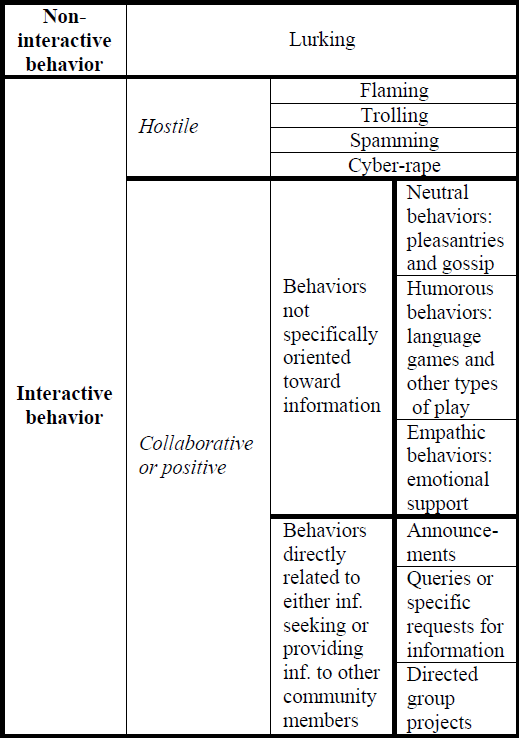
\includegraphics[width=0.45\textwidth]{../images/burnett.png}
\caption[Burnett's typology of online behaviour]{Burnett's typology of online behaviour (2000)}
\label{fig:burnett}
\end{figure}

\subsection{The changing face of \glsfmtshort{CMC}}

Between the mid 1990s and the mid 2000s, the nature of \gls{CMC}---and consequently, \gls{CMC} research---underwent a period of rapid change. As the result of a number of interwoven factors (the growing affordability of home computers; increasingly digital literacy; the development of early social network sites, etc.) the landscape of the Internet shifted from being primarily static and text\hyp{}based to dynamic, multimodal and participatory in nature \cite{herring_discourse_2011,lindholm_identity_2012}. The three currently most popular websites according to \emph{Alexa} in 2016 (\emph{Google}, \emph{YouTube} and \emph{Facebook}) exemplify this shift, in that each allows a great deal of user\hyp{}input and provides content in textual, audio and graphic modes. \textcite{herring_discourse_2011} reimagines the typology of familiar, adapted and new genres proposed by \textcite{crowston_reproduced_2000} to relate the dominant text types of `Web 2.0' to those that came before. Importantly, she notes that web genres can shift toward new\slash emergent as they mature, gaining features and responding to users' needs.

\subsubsection{Revisions of key claims in CMC research}

The profound nature of the shift to `Web 2.0' has meant that much early \gls{CMC} literature has now lost some of its relevance or explanatory power. Research into email messages is problematised by the fact that social media has overtaken email as the \gls{CMC} mode of choice for most digitally literate citizens \cite{thorne_computer-mediated_2008}, and by increasingly blurred boundaries between synchronous and asynchronous \glspl{mode}, such as email and instant messenger services. Similarly, the anonymity posited as critical to the discourse of early \gls{CMC}, while still possible, is no longer the norm: on social networking sites such as Facebook, \glslink{member}{users} communicate through personal accounts, disclosing their identities as they communicate and often even rendering the communication viewable to family and friends \cite{boyd_social_2007}. Furthermore, given that social networking sites are multimodal, and often contain a mixture of synchronous and asynchronous interactions, research informed by a characterisation of the Internet as fundamentally text\hyp{}based, or dealing exclusively with synchronous or asynchronous communication, is of limited usefulness for researchers of contemporary, often multimodal, \gls{CMC}.\endnote{For example, the myriad studies of communication on \emph{Usenet}---the text\hyp{}only Internet communication system in which many of the social elements of \gls{CMC} were first popularised---have been made largely redundant by the decommissioning of Usenet servers in 2010 \cite[e.g.][]{berge_computer-mediated_1995,eklundh_use_1994,jaffe_gender_1995}. That said, researchers have noted that despite greater bandwidth and the potential for multimodal interaction, in many respects, \gls{CMC} has remained surprisingly text\hyp{}based.}

In addition to the problem of reduced applicability, the findings of earlier research have since been challenged by research from the previous two decades \cite{herring_computer-mediated_2001,postmes_formation_2000}. As early as the mid 1990s, the characterisation of \gls{CMC} as impersonal, ineffective and hostile had come into question: \textcite{walther_computer-mediated_1996} argued that many early findings were caused by researchers' placing time restrictions on the observed \gls{CMC} interactions. If \gls{CMC} interactions are given unlimited time, Walther contends, they can achieve the same level of depth as face\hyp{}to\hyp{}face scenarios, both in terms of task\hyp{}completion and in the development of social relationships. In fact, Walther notes the potential for \emph{hyperpersonal} interaction in CMC: due to an optimised presentation of the self \cite[now often called \emph{self\hyp{}curation}; see][]{van_kleek_self_2015}, as well as idealisation of the Other, \gls{CMC} groups were found to be more polite and intimate than a face\hyp{}to\hyp{}face counterpart. Walther thus recognises two critical facts about interaction online: first, computer\hyp{}mediated interaction can be more candid than what could be observed in a comparable face\hyp{}to\hyp{}face setting; second, relationships develop in \gls{CMC} just as they do offline, necessitating longitudinal research. 

%From this perspective, aside from the slower pace of interactions, synchronous text\hyp{}based \gls{CMC} and face\hyp{}to\hyp{}face communication can be conceptualised as fundamentally similar in nature \cite{osullivan_reconceptualizing_2003,walther_interpersonal_1994,wu_is_2013}. The rapid increase in access to \gls{CMC} since this study 

The notion of a genderless and egalitarian Internet has faced similar scrutiny: \gls{CMC} research has shown that gender in anonymous, text\hyp{}only \gls{CMC} is often encoded by the \glslink{lexicogrammar}{lexicogrammatical} choices of the writer, as well as through the use of gendered discourse strategies such as assertiveness, politeness and aggression \cite{herring_gender_2000}. Likewise, education level is conveyed through vocabulary and complexity of message structure, and age through the discussion of interests and life experiences \cite{herring_computer-mediated_2001}. These findings echo the \glslink{SFL}{systemic-functional} notion that \emph{context is in text}, rather than around it, and can thus be reconstructed from linguistic analysis \cite[see Section \ref{sect:sfl}, as well as][]{eggins_introduction_2004}. Finally, research from the perspective of \gls{CDA} has questioned the notion of an egalitarian Internet at two separate levels. At the level of discourse, newer studies show that complex and rigid power structures exist online, even in low\hyp{}bandwidth \glspl{forum} and discussion lists \cite[e.g.][]{stommel_online_2010}. More broadly, contemporary theorists acknowledge that the landscape of \gls{CMC} has `inherit[ed] power asymmetries from the larger historical and economic context of the Internet', with a notable over-representation of English speaking, white males positioned as moderators, webmasters, and page creators \cite[p.~12]{herring_computer-mediated_2001}.

%Data and metadata are commodities: a main source of revenue for micro-blogging website Twitter is its \emph{Firehose}---an API that allows customers access to 500 million tweets per day. Researchers have attempted to mine tweets to detect natural disasters; to play the stockmarket; to aggregate content for entertainment websites. Each of these tasks requires the extraction of information from natural language.

\subsection{Contemporary CMC and its affordances for research}

%Though the Web is becoming more and more multimodal, methods for analysing human behaviour based on creation and consumption of multimodal content are only emerging. Multimodal content is very difficult to process automatically---typically, a great deal of manual effort is needed to transform multimodal content into data, and from data into insight. Plain text and metadata, however, are easier to transform into data, easier to annotate, and easier to search.

%todo: possible conflict between gruba and robyn re: future proofing ... i've deleted 'By 2016'
\gls{CMC} has now become become a central component of daily life, accounting for an ever\hyp{}increasing proportion of all human communication. Today, \gls{CMC} is used to contact those already close to us, rather than like\hyp{}minded strangers. Instead of well\hyp{}defined sessions of \gls{CMC} at a home computer, \gls{CMC} is now dispersed through work, travel and social occasions, and facilitated by an interconnected ecosystem of smartphones, tablets, laptops and desktop computers. Media convergence has led to new genres of communication, between journalists and readers, or companies and customers. The current Web therefore provides language examples that cannot be obtained through other means \cite{harvey_disclosures_2012}, or which have no antecedent in face\hyp{}to\hyp{}face discourse \cite{herring_discourse_2011}. As such, analysis of \gls{CMC} texts becomes necessary for investigation of many longstanding aims of linguistic research, including how language changes or evolves, how language is used to form and attend to social relationships \cite{canary_relationship_2015}, and\slash or how language is used to construe the human experience of the world.

\section{Healthcare and online communities}

% bit of a jump here ... 
Health discourse, in some form or another, is a large part of the landscape of contemporary \gls{CMC}---72 per cent of adult Internet users in the U.S. report having searched for health\hyp{}related content online \cite{fox_health_2013,fox_social_2014}. As mentioned in Chapter \ref{chap:intro}, talk about health covers a spectrum of registers \cite[in the systemic-functional sense\textemdash{}see][as well as Section \ref{sect:sfl}]{halliday_introduction_2004}. Ideationally, healthcare is a key topic online, with information about every conceivable symptom, illness and treatment strategy readily available through search engine results. Textually, health is represented in every popular \gls{mode} of \gls{CMC}, including wikis, blogs, online news, chatrooms, static information pages and mobile apps. Interpersonally, online health information targeting \glspl{consumer}%
\endnote{Interpersonally, not all health information online targets consumers---there are also sites with information for health professionals, academics, and so forth. These, however, are not relevant to the thesis.}
may be authored by governments, non\hyp{}profit organisations, health professionals, researchers, journalists, or, importantly, by healthcare consumers themselves. The latter of these---personal experiences with healthcare, authored by those living with health problems, and those who care for them, have significant public demand: a quarter of surveyed U.S. adults report specifically seeking out \glspl{consumer}' subjective accounts of their experiences with illnesses and journeys through healthcare systems \cite{fox_social_2014}.

Much consumer\hyp{}generated talk about health goes on inside dedicated online communities\textemdash{}that is, `mediated social spaces in the digital environment that allow groups to form and be sustained primarily through ongoing virtual communication processes' \cite[p.~986]{shen_effects_2013}. These communities most commonly exist within social networking sites (e.g. Facebook groups, Subreddits) or within bulletin board\slash \gls{forum} platforms\textemdash{}text-based \glspl{mode} of \gls{CMC} where registered \glslink{member}{users} can create and reply to \glspl{thread}. In academic literature and beyond, health\hyp{}oriented \glspl{forum} have been conceptualised as \glsxtrfullpl{OSG}\textemdash{}an online permutation of more traditional support networks for people living with health problems, or for those who care for them.

\glslink{forum}{Forum}\hyp{}based online communities and \glspl{OSG} have long been used as data sources for linguistic research due to their size, ubiquity and the ease with which they can be accessed: access to \glspl{forum} is round\hyp{}the\hyp{}clock and global; recording and transcription are unnecessary; and in many cases linguistic data is accompanied by rich, well\hyp{}structured demographic metadata \cite{leech_new_2006}. In general, empirical studies have shown that when contrasted with face\hyp{}to\hyp{}face equivalents, online communities have fewer barriers to entry, higher dropout rates and a comparatively high proportion of peripheral membership---that is, a greater rate of inexperienced or new members, compared to longstanding veterans \cite{sandaunet_challenge_2008,zhang_peripheral_2001}. That said, the efficacy of comparisons and contrasts between face\hyp{}to\hyp{}face and computer\hyp{}mediated communities has recently been questioned, as daily life becomes increasingly mediated by and merged with digital technologies \cite{wu_is_2013}. Indeed, a great number of users of \glspl{OSG} have never attended the offline antecedent of the \gls{mode}.

Linguists have paid attention to the central role played by language in online communities and \glspl{OSG}. It has long been argued by researchers that the limited semiotic resources available in many online environments (chiefly, a lack of physical co\hyp{}presence) makes language the most suitable resource for identity construction and role\hyp{}relationship negotiation \cite{thorne_computer-mediated_2008}. As \textcite[p.~303]{lam_language_2008} notes, `language practices are instrumental in creating the norms of behavior of particular online groups and how these norms function to provide sociability, support, information, and a sense of collective identity'. A similar perspective is provided by \textcite{postmes_formation_2000}, who argues that social identity issues have a stronger presence in \gls{CMC} environments, due to the de\hyp{}individuation that occurs in part due to reduced cues online. Because \glspl{OSG} facilitate intra\hyp{}consumer exchange, and because of the centrality of language to this task, the main thrust of linguistic online community and \gls{OSG} research has been toward language as an interpersonal, rather than an ideational resource---that is, toward the ways in which language is used to enact social relationships, rather than as a means of construing reality. Many studies have focussed on differences in communicative practices over the course of membership\textemdash{}most typically, on how newcomers position themselves as legitimate prospective members whose contributions deserve replies, and how longer\hyp{}term members represent their expertise and construct\slash reinforce normative community values. In the sections that follow, I review key \glspl{theme} in linguistic accounts of interpersonal meaning\hyp{}making in online communities, with preference given to \gls{forum}\hyp{}based or health\hyp{}oriented communities where available.

%In health contexts, the centrality language provides an attractive possibility for research into \gls{consumercentred} care, which similarity shares an interest in interpersonal, rather than ideational meaning\hyp{}making. % includes section on online community

%\input{chapters/cmd.tex}

% NEW MEMBERS
    % legitimacy

% VETERAN MEMBERS
    % van leeuwen
    % legitimacy
    % the lay expert

% LONGITUDINAL CHANGE
    % socialisation

% SHORTCOMINGS
    % qualitative
    % non-systemic

%todo: add %\textcite{pfeil_social_2011} show how core community members are more likely to adopt supporting
% Though we can easily infer longitudinal change in members' roles, the authors do not show this process occurring.


\subsection{New members, first contributions and legitimacy} \label{sect:newmembers}

People can sign up and begin contributing to most \glspl{OSG} at any time. A common practice is for new \glslink{member}{users} to create a new \gls{thread}, which serves as a self\hyp{}introduction, often outlining the user's motivation for having joined. Because drop\hyp{}out rates are high, such `first \gls{post} \glspl{thread}' are a constant feature in the landscape of many popular \glspl{forum}, and have thus received attention during studies of \glspl{OSG}.

There are broad interpersonal similarities between first contributions within many \glspl{OSG}. Generally speaking, new users attempt to carve out a social position from which it is possible to elicit certain kinds of language from others\textemdash{}that is, to increase the perlocutionary force of one's own utterances \cite{austin_how_1975,roberts_communicative_1996}. Most commonly, new \glslink{member}{users} want to be given information and social support after having requested it. This has been referred to as a position of \emph{legitimacy}, arrived at through an ongoing process of \emph{legitimation} through semiotic exchange \cite{davies_communities_2005,smithson_developing_2012,van_leeuwen_legitimation_2007}. In comparison to offline support groups, where physical co\hyp{}presence and extralinguistic communication can serve legitimating functions, new contributors to \glspl{OSG} instead exchange meaning and communicate legitimacy almost exclusively through the linguistic content of their \glspl{post} \cite{galegher_legitimacy_1998}. The kinds of language choices that manoeuvre the \glslink{member}{user} into the legitimate position may vary, with individual community cultures shaping what messages contain, how messages are structured, and the kinds of replies they receive \cite{gallagher_what_2015}.

\subsubsection{Legitimation strategies in newcomer talk}

Because texts are structured in order to make things happen, and because one of the functions of first \glspl{post} is to legitimate the self, it is possible to look within the structure of these texts to see how legitimation is realised at the strata of \gls{lexicogrammar} and \glspl{discourse-semantic}. Commonly, first \glspl{post} are designed to demonstrate the fulfillment of explicit, implicit or perceived community membership criteria. \textcite{varga2014grieving} qualitatively analysed more than 100 first \glspl{post} to an \gls{OSG} for grief, unpacking the ways in which new users socially construct grief in a way that elicits useful responses. Three main strategies were identified: presentation of an atypical story, presentation of an uncontrollable emotional state, and through \emph{troubles telling}\textemdash{}\glspl{post} in which the new \glslink{member}{user} explains a problem but does not explicitly request advice.
%The analysis of pairs of request and response is indeed the best way to obtain a useful sketch of the ways in which advice is dispensed, and the underlying motivations for each choice. This kind of approach also poses problems for \gls{CL} methods, however, as few \gls{corpus} are annotated in such a way as to link the initialisation and response components of the text.

Similarly, \textcite{smithson_membership_2011} describes the legitimating function of first \glspl{post} to an \gls{OSG} for self\hyp{}harm: new \glspl{member} were observed setting out their credentials for group membership, giving narrative medical histories, utilising medical jargon and making reference to other related communities in which they have participated. This finding is echoed by \textcite[p.~5]{varga2014grieving}, who find that `story formulations often serve particular functions in discourse, such as displaying affiliation with a group and establishing eligibility for group membership'.

\textcite[p.~173]{horne_doing_2009} use discursive psychology as an underlying theoretical framework to analyse the structural and functional components of first \glspl{post} to a suicide \gls{OSG}. They explore the difficulty faced by \glspl{member} who present as suicidal, but whose continued presence in the \gls{forum} casts doubt upon the legitimacy of their claim. Three major types of messages are identified: \emph{life narratives}, in which a medical history is presented without a specific addressee; \emph{immediate threats}, which are typically short, containing present and future tense; and \emph{requests}, which involved requests for advice, and the use of mainstream medical terminology. The latter category received the fewest replies. The authors hypothesise that this is due to a lack of urgency within the lexicogrammatical choices of \emph{request} \glspl{post}, leading to an impression that the new \gls{member} is `inauthentically suicidal' \parencite*[p.~180]{horne_doing_2009}. At the same time, explicit requests for advice construct potential responders as equally inauthentic, as it casts them as using the \gls{OSG} for purposes other than support seeking. 

\textcite{stommel_use_2011} adopt \gls{CA} as a way of showing how new \glslink{member}{users} in an eating disorder \gls{forum} engage in self\hyp{}legitimation by representing themselves as having been formally diagnosed with a disorder. While having a diagnosis is not an explicit community rule, the authors argue that it nonetheless functions as an `entry ticket' for continued participation within the group \parencite*[p.~6]{stommel_use_2011}. Though this is an interesting suggestion, so far lacking is a detailed investigation of the syntagmatic behaviour of the diagnosis event as it is construed in \gls{OSG} texts: if the process of diagnosis functions as an `entry ticket', we might expect that it is construed metaphorically as a participant, so that it can be classified and possessed.

In the same paper, \citeauthor{stommel_use_2011} also show how newcomers often express reluctance to participate and insecurity concerning the content of their first \gls{post}. These hesitations are marked in  the lexicogrammar, by modal auxiliaries and adjuncts, and by ellipsis, which may be marked graphologically with ellipses (e.g. \emph{I'm still a bit unsure about what I should write \dots}). The authors argue that marking hesitation allows the new user to appear equitable and well\hyp{}prepared. At the same time, hesitation is argued to indicate a level of respect for the opinions of the rest of the community, communicating an intent to take replies seriously. 

\subsubsection{Structure of first posts} \label{sect:post-structure}

Some authors have commented on the overall structure of first posts. \textcite{varga2014grieving}, for example, note that new threads posted to the \gls{OSG} for grief often conform to common structure:

\begin{quote}\small\singlespacing
We found that newcomers opened their initial \glspl{post} with stories that began at the event of loss and then moved to establish the background of their relationship with the deceased. Emphasizing the unusual circumstances of their loss and the depth of their connection with the deceased provided an account for their grief. Newcomers continued their accounts through descriptions of their uncontrollable emotional and physical symptoms, which worked to display affiliation with \glspl{member} of the group and to make the case for their legitimate entry \parencite*[p.~5]{varga2014grieving}. 
\end{quote}
%
%\noindent The authors point out, however, that their qualitative approach limits the generalisability of the study, noting that further research is necessary to confirm their exploratory results.
%
Similar structural components---the narration of a personal (medical) history, and its lead\hyp{}up to a current problem---have been identified in other analyses of \glspl{OSG}. \textcite[p.~4]{weber_missed_2011} analyses the role of dispute and conflict in the socialisation process of new \glspl{member} of an online sexual abuse support group. She provides a basic account of the generic structure of newcomers' \glspl{post}:

\begin{quote}\small\singlespacing
Contents typically found in newcomers' messages include: a greeting; a description of the person's contact with the group thus far; a reference to sexual abuse experiences or related problems; and a request.
\end{quote}
%
Using terminology from \textcite{goffman_presentation_1959} and \textcite{brown_politeness:_1987}, Weber makes a case that this structure represents an \emph{entrance frame}: during each component of the frame, devices such as humour, insecurity, and unease can be used to both perform identity and to set up an exchange with a lessened potential for loss of face or redress. 

%todo: clarify typographical conventions
Using the framework for narrative stage analysis outlined by \textcite{labov_narrative_1997}, \textcite{kouper_pragmatics_2010} provides an account of the structure of initial \glspl{post} to a \emph{LiveJournal} community. She notes that messages contain sequences of \sctext{ORIENTATION}, \sctext{PROBLEM DISCLOSURE}, \sctext{REQUESTS} (for advice and for information; of varying degrees of explicitness) and \sctext{JUSTIFICATION} for posting. Because there was no hard limit on the size of a contribution (as is typical of \glspl{OSG}), all stages aside from the \sctext{ORIENTATION} can occur multiple times in a single text. No component was found to be obligatory in every message.

%Because it is possible to remain a lurker in many \glspl{OSG}, the act of self-introduction itself, irrespective of its linguistic content, is an act that demonstrates desire for membership.

\subsubsection{Limitations in current understanding of newcomer talk} \label{sect:limit-newcomer}

% not really important ...
A potential methodological issue in the work of \textcite{horne_doing_2009} \citeNP[as well as others, e.g.][]{stommel_online_2010} is that the authors treat the presence or absence of replies as indicators of a \gls{post}'s `success'. While this may be a sensible or convenient assumption when doing larger, quantitative\hyp{}based studies of number of replies, it is perhaps less reliable in small\hyp{}scale qualitative research: there is no explicit evidence concerning whether or not replies would have been posted if the first \gls{post} were written differently. Moreover, when using publicly available \gls{forum} data, there is no reliable way to tell that \glspl{post} were even seen by those who would be likely to reply. Another key factor in whether or not replies are received is the user's profile: \textcite{feng_is_2016} find that \gls{OSG} participants with recoverable first names and portraits as avatars receive friendlier, more personalised replies than do more highly anonymised users. In general, however, this factor has not been taken into account in related literature.

%\textemdash{}a phenomenon known as \emph{lurking} common to many \glspl{mode} of \gls{CMC}
A second key issue in the study of new \glspl{member} and initial contributions is the potential for a user's first experience with the community and his\slash her first contribution to it to be conflated. Though first \glspl{post} represent the first time a user actively engages in a discussion, he\slash she may not in fact be new to the community: a user may have signed up or read through \glspl{thread} for any length of time before choosing to 
\gls{post}. Some first contributions, therefore, are made by people who have just discovered the community and are unaware of its normative communicative practices, while others are made by \glspl{member} who are already intimately familiar with the community's discursive norms \cite{dennen_pedagogical_2008,han_social_2012,preece_top_2004,smithson_membership_2011}. \textcite{weber_missed_2011}, for example, shows that long\hyp{}time lurkers often draw upon the normative genre and register appropriately when they first decide to author a \gls{post}. Such \glslink{member}{users}, she finds, often flag in their \glspl{post} the fact that they have lurked for extended periods before posting, in order to account for their level of familiarity with the lexicogrammatical, discursive or ideological orientation of the group. The phenomenon of lurking therefore poses a specific challenge to particular theoretical conceptualisations of group dynamics. Socialisation theory, for example, in stressing the notion of learning through active participation, may become an unsuitable model for interpreting communities where a great deal of learning may take place non\hyp{}interactively.
% Reasons for this are potentially contradictory: users may flag their newcomer status in order to provide a reason for their breaking explicit or implicit community rules; alternatively, user
%for approaches to online community\slash\gls{OSG} membership informed by socialisation theory, for example ow), which stresses the process of learning through active participation.

A final limitation in existing work on first posts to \glspl{OSG} is the dominance of bottom\hyp{}up, \gls{CA}\hyp{}informed approaches. While \gls{CA} is certainly suitable for exploratory, qualitative and discourse\hyp{}analytic work, it is not intended to uncover generalisable relationships between linguistic system and language instance. For this reason, \gls{CA} is not typically used in large\hyp{}scale quantitative investigations, which access discourse through automatic location of lexicogrammatical phenomena, and manual abstraction of the meaning of these phenomena via a grammar. \gls{CA}, therefore, while useful as a way of identifying legitimation strategies, has not provided an explicit description of how legitimation may be realised in words and wordings. This limits the ability to perform automated feature discovery or frequency counting, as well as the ability to uncover register differences based on fluctuations in frequencies of lexicogrammatical phenomena.

\subsection{Veteran membership and legitimacy} \label{sect:vetmemb}

A smaller proportion of \gls{OSG} legitimacy research has concerned the language use of veteran members, especially as replies to initial contributions \cite{paulus_`please_2015}. As noted in Section \ref{sect:intro-lang-in-osg}, these studies address a hypothesised concern from earlier \gls{CMC} theory that \glspl{member} may take advantage of the lack of social cues in the online community and linguistically convey a level of expertise or legitimacy at odds with their actual level of health literacy or knowledge \cite{varga2014grieving}. Evidence regarding the existence and ramifications of this phenomenon is conflicting, however \cite{sillence_giving_2013}. \textcite{hoch_information_1999}, for example, found that six per cent of all advice provided in an epilepsy \gls{forum} was objectively wrong. Similarly, \textcite{hoffman-goetz_clinical_2009} concluded that nine per cent of information in a diabetes community deviated from clinicians' guidelines. On the other hand, Sillence's study of a breast cancer \gls{forum} found that `only a very small amount of messages observed in the present study reflected a lay belief or misbelief in [patient-controlled analgesia] treatment' \parencite*[p.~8]{sillence_communicating_2012}. \textcite{smithson_problem_2011} reported that in contrast with researchers' expectations, replies to new \glspl{member} of a self\hyp{}harm \gls{forum} were almost always found to be surprisingly mundane and conservative in nature, with `go and visit the GP' being by far the most common advice dispensed. Research has also yet to show a conclusive link between incorrect or poor quality information online and negative treatment outcomes. As \citeauthor{wang_stay_2012} explains:

\begin{quote}\small\singlespacing
It is highly likely that the effectiveness of such groups depends on the communications that \glspl{member} exchange with one another, but surprisingly little systematic research has been devoted to specifying how the quality and quantity of such communications affect groups' outcomes and members' health\hyp{}related outcomes \parencite*[p.~1]{wang_stay_2012}.
\end{quote}

In general, analyses of \glspl{OSG} have shown that long\hyp{}term \gls{forum} \glspl{member}' language use differs from that of newcomers in a number of respects. Veterans are more likely to welcome newcomers, speak on behalf of the \gls{forum} and its other members, dispense advice and instructions, and\slash or act as gatekeepers by ratifying or rejecting membership bids \cite{paulus_`please_2015,pederson_supporting_2010,weber_missed_2011}. As such, these \glspl{member} are usually understood as being in a position of power, or higher social standing, than the newcomers they address.

Inspired in part by \gls{SFL} theory, \textcite[p.~92]{van_leeuwen_legitimation_2007} proposes four major discursive strategies for legitimation used by those in positions of power: \emph{authorisation} (reference to `persons in whom institutional authority of some kind is vested', potentially including both the speaker him\slash herself and\slash or those with whom he\slash she agrees), \emph{moral evaluation} (reference to venerated social values), \emph{rationalisation} (references to hegemonic social action) and \emph{mythopoesis} (narratives casting legitimate action and those who perform them in a favourable light). Informed by \gls{SFL} and \gls{CDA}, \textcite{reyes_strategies_2011} augments Van Leeuwen's framework for the purposes of accounting more specifically for the ways in which social actors construct legitimate action through the use of emotion, the description of hypothetical future outcomes, and through displays of altruism. % [p.~782] -- reyes page

%Realisations of these strategies in grammar are diverse. % The appraisal framework is useful as a means of analysing emotional language;

The kinds of legitimation strategies described by \textcite{van_leeuwen_legitimation_2007} and \textcite{reyes_strategies_2011} have been empirically observed in the language of those who respond to newcomers' \glspl{post}. Particularly relevant is legitimation via reference to personal authority. First, a number of studies have highlighted the framing of health professionals as authorities. \textcite{smithson_problem_2011} and \textcite{vayreda_social_2009} have found that advice dispensed by veterans often aligns with a biomedical ideology, in which the health professional is the definitive source of knowledge, as well as the agent behind critical points in the consumer journey such as diagnosis. Second is the framing of the self and other veteran \glspl{member} as authoritative. Van Leeuwen distinguishes between three different subtypes of authoritative legitimation: \sctext{personal} (in which the authority figure and the target are in a culturally recognised hierarchical relationship, such as student\slash teacher or child\slash parent), \sctext{expert} (where the authority figure has relevant experience that is lacking for the target) and \sctext{role model} authority, where actions are justified on the basis that they are also performed by people that the target may respect or admire). Grammatically, authoritative legitimacy often involves verbal and mental processes with the authority positioned as Sayer\slash Senser. The personal subtype is likely to also involve high\hyp{}obligation modality (\emph{she said that we should go}\textemdash{}see Section \ref{sect:sfl} for an elaboration of the \gls{SFG}). Veteran \gls{OSG} \glspl{member} have been shown to variously fulfill each of the three subtypes. They may explicitly moderate problematic content or ban \glslink{member}{users} who break rules \cite{weber_missed_2011}. They may provide expertise by providing health information in an objective, impersonal Tenor, as a set of facts \cite{kaufman2016producing}. Alternatively, they may self\hyp{}present as role models, providing health information and advice alongside personal narratives from their ongoing consumer journey \cite{koteyko2015performing}.

%Appeals to tradition and conformity
%The notion of legitimacy can be applied here too; that said, the strategies for becoming legitimate are generally different, as are the desired perlocutionary effects that come from the legi
%Veteran \glspl{member} may want to have a say in the overall direction of the community; they want their demands on others (advice giving, or requests for follow-up information) to be heeded.
%As \textcite{eggins_analysing_2004} point out, understanding the ways a text is responded to is key to understanding its original purpose. \textcite{harrison2009politeness} note that phenomena such as politeness and advice are bound to context; interpretation of the ways people react to others is critical to proper understanding of intentionality.

\textcite{kaufman2016producing} use a combination of \gls{CA} and discursive psychology to analyse replies in an \gls{OSG} for depression and their usefulness as social support devices. They note that responders to first \glspl{post} communicate empathy through a two\hyp{}part structure of explicitly claiming to feel empathy (e.g. \emph{I feel the same way}) followed by a demonstration of a shared trouble, and, potentially, a construal of the speaker as role model. An example from their data demonstrates this structure clearly:

\begin{quote}\small\singlespacing
I went through the same things that you are going through right now about 2 years ago. I PROMISE you that things will get better. The way that got me out of being depressed is by taking out my anger and sadness on making music or writing stuff down on some paper \parencite*[p.~8]{kaufman2016producing} 
\end{quote}
%
Unlike most \glspl{OSG} research, the authors problematise the distinction between information and support provision: in cases such as depression, psychoeducation can relieve symptoms by normalising the experiences of the addressee. As such, even objectively presented health information functions as a gesture of social support. Likewise, the authors point out the reciprocal nature of offers of empathy within the depression community. Those who respond to new \glspl{thread} (most typically, veteran \glspl{member}) are also benefiting from the exchange, in being given a platform and space in which they can engage in a kind of talk therapy. As such, provision of support by veteran \glspl{member} may simultaneously affect the second person (the addressee), the third person (other community \glspl{member} and readers) and the first person (the self). More directly, \textcite{pudlinski_giving_1998} has shown that sharing related stories may in fact elicit direct social support from the addressee. In this way, part of the motivation for the responder is to receive the same manner of support that he\slash she is providing in the response.

%They note that lacking in the existing literature have been analyses that connect features of \gls{OSG} texts to the efficacy of the communities as sites of social support.

\subsubsection{Advice} \label{sect:advice}

Either explicitly or implicitly, studies of replies and\slash or veteran \gls{member} behaviour in \glspl{OSG} have often centred on the notion of \emph{advice}. Defined here as `opinions or counsel given by people who perceive themselves as knowledgeable, and\slash or who the advice seeker may think are credible, trustworthy and reliable' \cite[a definition taken from][p.~519]{decapua_strategies_1993}, advice is interesting due to its inherent ties to legitimacy, and due to its multifunctionality: advice has both interpersonal purposes (to cause the addressee to do something; to negotiate power dynamics) and experiential purposes (to construe facts and\slash or ideal behaviour) \cite{heritage_dilemmas_1992}. Peer\hyp{}to\hyp{}peer advice is also important for clinical research, given its potential influence over \glslink{member}{users}' healthcare decision making practices \cite{jones_health_2013,sillence_giving_2013}.

Linguistic perspectives on advice provision in English have been provided by \textcite{hudson1990discourse}, \textcite{decapua_`if_1995} and \textcite{decapua_strategies_1993}. Generally, the focus of these accounts has been on the directness of advice, whether or not it was solicited, and the influence of these factors on how it is received. Common is the recognition that advice is potentially face\hyp{}threatening, and as such, its realisations are diffuse within the grammar. Advice is often accompanied by hedging strategies, including incongruent mood choices, modalisation, or politeness markers: `even solicited advice\hyp{}givers can resort to a variety of stylistic and linguistic means to protect themselves from accusations of unfairly taking on the role of ratified experts' \cite[p.~126]{decapua_`if_1995}. A given instance of advice may therefore have agnate realisations as an imperative (\emph{Go and make an appointment}), a declarative (\emph{You should make an appointment}) or an interrogative (\emph{Could you make an appointment?}).

\textcite{kouper_pragmatics_2010} investigates an online motherhood community hosted by \emph{LiveJournal}, focussing on both realised forms of advice, and on the structure of the \glslink{post}{text} to which the advice giver is responding (see Section \ref{sect:newmembers} for studies of first \glspl{post}). Occurrences of advice in a one\hyp{}month sample of contributions were coded according to four categories: 

\begin{enumerate}\small
\item Direct advice (Any comment that included imperatives or the modal verb \emph{should})
\item Hedged advice (Any comment that contained explicit hedges, hedging devices, or softeners of various types)
\item Indirect advice (Any comment that had no explicit or hedged advice, but had enough information to act on it)
\item Description of personal experience (Any comment that had no explicit, hedged advice, or indirect advice, but had an account of how the person dealt with the situation an advice seeker had described) \cite[adapted from][p.~7]{kouper_pragmatics_2010}
\end{enumerate}
%
The categories are primarily designed to distinguish directness of advice, with grammatical distinctions naturally playing an important, but secondary role. Notably, imperative and \emph{should}-modalised declarative are understood as equally direct---a classification at odds with the \gls{SFG}, where \sctext{Modality} is a more delicate grammatical component than Mood Type. Also of interest to the case study of this thesis and its associated methods is the most indirect kind of advice, which has no explicit grammatical criteria. An example is provided:

\begin{quote}\singlespacing\small
beautiful becca :) i gave wesley a bath every 2-3 days. but now he is 10 weeks old and i bathe him every night because he loves his bath time so much  \textcite[p.~13]{kouper_pragmatics_2010}.
\end{quote}
%
Naturally, such indirect realisations are a complicating factor for \gls{CL} approaches to advice, which may struggle to automatically locate instances that are not indexed by any one particular \glslink{lexicogrammar}{lexicogrammatical} feature. This is discussed in more detail in Chapter \ref{chap:discuss-bp}.

Advice research has also highlighted the fact that strategies for advice provision are affected by the roles and relationships of interactants. \textcite{decapua_`if_1995} show how the use of unhedged imperatives, for example, is more likely in contexts where the difference in status between advice giver and receiver is obvious, explicit and\slash or institutionally prescribed. Interactions between speakers of similar social standing are more likely to feature more hedging, including modalisation, and declarative Mood. In such contexts, \citeauthor{decapua_`if_1995} note, advice giving and requesting can foster interpersonal closeness through \emph{(i)} the determination and exchange of shared values, \emph{(ii)} flattery, by a positioning of the advice giver as knowledgeable, and \emph{(iii)} potentially intimate personal revelations.

% LOCHER
Advice online has been investigated extensively by Locher \parencite*{locher2006advice,locher_health_2010}, focussing mostly on an online advice column called \emph{Lucy Answers}. Locher's interest is primarily in what she calls \emph{interpersonal pragmatics} or \emph{relational work}---what may in \gls{SFL} be understood as \emph{interpersonal \glspl{discourse-semantic} or meaning}. Her approach relies on manual annotation of various syntactic and semantic features of the questions asked to the columnist and her replies. 

For her analysis of relational work, Locher codes the columnist's responses with seven relatively broad semantic categories: \emph{bonding}, \emph{boosting}, \emph{hedging}, \emph{praising}, \emph{emphasizing}, \emph{criticizing}, and \emph{humor}. Categories may contain subcategories (to reflect, for example, the hedging function of humour), and multiple categories may be applied to a part of a text. She finds that hedging is a very common strategy, related to the overall genre of the column. Lucy the advice giver fosters a sympathetic relationship with readers and contributors, rather than a hierarchical one. Hedging lessens the difference in social status that may stifle the candid kinds of language use that the column's readers enjoy. These categories differ in the extent to which they can be mapped to particular features of the \gls{lexicogrammar}: Locher's examples of hedging are typically examples of modulation (\emph{maybe}) or modulation via grammatical metaphor (\emph{It is important that you ...}); \emph{humor}, however, mostly relies on the judgement of the analyst, the recognition of wordplay, and the like. Because these kinds of features differ in the extent to which they are indexed in grammar, they also differ in the extent to which they can be identified automatically using computational tools and methods.

\textcite{locher2006advice} also employs counting of lexicogrammatical features, which can more reliably be counted using methods from \gls{CL}. When analysing the ways in which Lucy dispenses advice, Locher codes texts for Mood Type, finding that declaratives, often modalised, are the most common (52\%), followed by imperatives (36\%), and interrogatives (11\%). These results are contrasted with other studies of advice in contexts such as face\hyp{}to\hyp{}face or radio, which more commonly feature imperative realisations. She argues that the orientation of the advice column `toward facilitating decision processes' (p.~132) is responsible. In situations where the potential for losing face is less critical than effective prescription of a course of future behaviour, direct forms are likely to be preferred.

%in high-stakes, professional--consumer medical contexts, for example, 

There are two major limitations in Locher's work for investigating advice in online health communities. First are apparent inconsistencies and contradictions in Locher's lexicogrammatical analyses. In the context of advice, Locher analyses declarative as being `suggestions', interrogatives as `inviting future action', and imperatives as `directives'. Because some examples of declaratives appear to be directives (\emph{You need to go ...}), however, Locher reclassifies declarative $+$ \emph{need}\slash \emph{should} as imperatives, arguing that `in written sources such as advice columns, a preference for imperatives and imperatives with \emph{should} or \emph{need} was found' (p.~39), despite the fact that \emph{should} cannot grammatically modalise an imperative clause. This is a conflation of grammatical Mood Type (imperative) and the speech function it typically realises (a command). A related issue is the conceptualisation of \emph{hedging} as a phenomenon distinct from Mood Type choice. Advice such as \emph{See your doctor}, when realised as an interrogative (\emph{Would you consider seeing a doctor?}) is perhaps better understood as a hedged form of the congruent command---especially in the advice column genre, where the question cannot possibly receive an answer.

%`When declarative sentences are used to realize advice, they can best be described as suggestions. (p.~192)

The second issue is that there are a number of critical medium and situational factors that differentiate online (forum\hyp{}based) communities from the \emph{Lucy Answers} online advice column. These differences can be understood with reference to the register dimensions of Tenor, Mode and Field from systemic linguistics \cite{halliday_language_1989}. In terms of Tenor, the advice column is an interaction between a pseudonymous advice seeker living with a health problem and a named, institutionally prescribed expert, who is responsible for selecting questions for publication and response. This power imbalance is likely to manifest in the ways in which advice provision is distributed amongst \sctext{Mood} and \sctext{Modality} systems: following \textcite{decapua_`if_1995}, we could expect that imperative provision of advice, for example, would be more common within the \emph{Lucy Answers} dataset than in most online \glspl{forum}, where contributors share a common identity as sufferers of a condition, differentiated hierarchically only by membership length and number of \glspl{post}, rather than by codified institutional roles. In terms of Mode, interactions within the advice column are limited to an initial question and a single response---in many respects, a reconfiguration of the advice column genre found in newspapers and magazines \cite[see][]{herring_discourse_2011}. As such, there is no longitudinal development and negotiation of role\hyp{}relationships between the two interactants, nor any way to track the health journey of the advice seekers after their contribution has been made. Compared with Tenor and Mode, the dimension of Field remains more or less consistent, however, with both \emph{Lucy Answers} and online health \glspl{forum} broaching a broad array of topics related to not just health, but work and social relationships as well. Though \emph{Lucy Answers} is unlike most health \glspl{forum} in not being dedicated to a single health concern, this is likely to affect only the ideational meaning embedded in advice (i.e. the specific health problem and remedial action construed), and not the ways in which advice is interactively exchanged.

% weird 1 appearing in harrison brackets
Related to Locher's work is that of \textcite{harrison2009politeness}, who investigate the linguistic negotiation of role\hyp{}relationships in an online community for arthritis. They categorise 255 advice moves by Mood Type using the same criteria as \textcite{locher2006advice}. Their findings are similar, with declaratives the most common (64\%), followed by imperatives (21\%) and interrogatives (15\%). They argue that this range of possible realisations is linked to the multifunctionality of the act: advice provides suggestions for future action while also reinforcing the veteran's claim to authority, and thus maintaining the hierarchical relationship between newcomer and veterans:

\begin{quote}\small\singlespacing
[Instances of advice] embody suggestions, while at the same time evidencing the writer's authority to make these suggestions: the narrative demonstrates the writer's experience of the recipient's problem, and the writer's chosen way of addressing the problem. Thus, through their narratives, the advice givers reflect on and give structure to their own experience, constructing their identities as expert patients \cite[p.~107]{harrison2009politeness}.
\end{quote}
%
While this study addresses the aforementioned concerns regarding the generalisability of Locher's work, and while it acknowledges the concurrent unfolding of interpersonal and ideational meanings in language, it nonetheless still provides only a general impression of the \sctext{Mood} and \sctext{Modality} probabilities of advice in online health \glspl{forum}: as with \textcite{locher2006advice}, \citeauthor{harrison2009politeness} do not provide a longitudinal account of interpersonal meaning\hyp{}making, nor an empirical account of the relationship between interpersonal status and lexicogrammatical choices.

Particularly relevant to this thesis is the study of a \gls{bipolar} \gls{forum} undertaken by \citeauthor{vayreda_social_2009}, which uses \gls{CA} to explore `an apparent contradiction between a new user's first post and \gls{forum} members' replies with ostensibly unsolicited advice' \parencite*[p.~931]{vayreda_social_2009}. It was found that new forum \glslink{member}{users} rarely explicitly asked for advice, but were provided with it regardless. The authors contend that advice was thus unsolicited, but complementary nonetheless: new \glslink{member}{users} made a `low bid' by only vague specification of the kinds of replies they sought; established \glslink{member}{users} took this opportunity to direct the user to shift toward group norms \parencite*[p.~940]{vayreda_social_2009}. This contrasts with \citeauthor{kouper_pragmatics_2010}'s finding that most advice was in fact solicited by the user who began the \gls{thread}. This contradiction is perhaps the result of the fact that \citeauthor{vayreda_social_2009} take a very narrow view of what exactly constitutes a request for advice, discounting formulations in which requests may be incongruently realised, as in the following:

\begin{quote}\small\singlespacing
`It'd be great if someone could share this first stage of acceptance with me, or tell me how they got through it.' \parencite*[p.~11]{vayreda_social_2009}
\end{quote} 
%
\noindent Here, though the new \glslink{member}{user} chooses a conditional declarative rather than a modalised interrogative as a means of realising a request, given that requesting advice involves deference and a potential loss of face \cite{brown_politeness:_1987}, such hedging does not seem inappropriate. Aware of the fact that expert \glspl{member} are fluent in the community's discursive norms, a new member could perhaps expect that such heavily modalised constructions could be unpacked and decoded as requests for advice. As \textcite{goldsmith2000soliciting} points out, while overt requests for advice open up a dynamic in which advice can be provided without threatening face, general solicitation of opinions on a topic are often understood by the addressee as permission to advise. In a hierarchical community of newcomers and experts, this is especially likely, as the new \glslink{member}{user} understands that the veteran has personal experience with the nature of the problem. As \textcite{eggins_analysing_2004} remind us, rather than relying on linguistic intuition alone, the best way to disinter the intentionality of an utterance is often to analyse the utterances that follow. Given that such responses are apparently treated as advice by those who respond, this may suggest an underlying shortcoming in Vayreda and Antaki's classificatory scheme.

\subsubsection{The lay-expert\slash proto-professional}

In medical contexts, a well\hyp{}noted strategy for legitimation is the invocation of a \emph{lay\hyp{}expert} or \emph{proto\hyp{}professional} register, which is realised at both \glslink{lexicogrammar}{lexicogrammatical} and \gls{discourse-semantic} levels. Lexically, for example, such a register may involve the use or appropriation of medical jargon in lieu of lay terms \cite{harvey_disclosures_2012,sullivan_gendered_2003}; discursively, the lay\hyp{}expert has been shown to foreground personal experience and display emotional affect when construing medical fields \cite{wilson_expert_2007}. This conceptualisation, of a social role and associated linguistic repertoire that lies between novice and expert, is one useful lens through which we can understand language features of long\hyp{}term \gls{OSG} members.

\textcite{thompson_credibility_2012} examine the discursive features of lay expertise through interviews with members of \emph{patient and public involvement panels}\textemdash{}laypeople consulted by medical institutions in the U.K. in an attempt to involve the public in the medical research process. They noted that those in lay\hyp{}expert positions may champion their lack of formal medical training or employment, arguing that it affords a unique point of view that is uncorrupted by financial or socio\hyp{}political factors. Simultaneously, a high degree of deference to the opinions of health professionals was also observed: interviewed participants `not only supported the dominant techno\hyp{}scientific discourse around research, but also seemed to defer readily to it in place of their own experiential expertise' \parencite*[p.~609]{thompson_credibility_2012}. That said, these findings may be strongly influenced by the social context in which the interviews took place: as the participants of the study were afforded privileges and treated as having `honorary' roles by health professionals, their construction of both their unique perspective and health professionals' ultimate superiority may be influenced by the desire to maintain their current position and role. Indeed, studies of \glspl{OSG} where normative community values oppose those of mainstream Western medicine have noted that formal healthcare institutions, their participants and processes (e.g. hospitals, health professionals and diagnosis) are often cast in a negative light and treated sceptically by community members \cite{mulveen_interpretative_2006}. One of the advantages of \glspl{OSG} as sources of data, therefore, is access to the lay\hyp{}expert register uncorrupted by the presence and potential influence of healthcare professionals.

%Related is the already\hyp{}noted finding in \textcite{horne_doing_2009} that \gls{OSG} \glspl{post} aligned with mainstream opinion and featuring information about doctors' diagnoses were ignored by other \glspl{member}.

%In a \gls{CMC} context, \textcite{paulus_`please_2015} refer to `second\hyp{}stories', where veteran responses to newcomers' introductory narratives involve telling similar or related narratives from the journey of the veteran. These tales serve to normalise the new \glslink{member}{user's} problem and promote solidarity. Simultaneously, such stories have legitimating functions: they establish lay expertise

%Veteran \glspl{member} also speak on behalf of the community, by welcoming, or by explaining the purpose and orientation of the community:

%Veteran users perform legitimation through rationalisation, construing new users' actions and feelings as in line with the hegemonic social values of the board. \textcite{paulus_`please_2015} give the example of 

\textcite{koteyko2015performing} operationalise the notion of the lay\hyp{}expert in an online context, using ethnography and text analysis to qualitatively examine the ways in which Facebook users construct a representation of the self as a lay\hyp{}expert in communication about diabetes. Noting that social networking sites have received less attention within online health discourse literature than \gls{forum}\hyp{}based communities, they argue that such sites provide new, under\hyp{}researched channels through which semiotic health resources can be exchanged. The convergence of a number of (monomodal and multimodal) types of \gls{CMC} within Facebook's infrastructure (e.g. link sharing, microblogging, chat, photo albums, etc.), for example, gives rise to a novel practice where users publicly share links to medical literature, accompanied by a `translation' or summary of its significance into simpler English for a lay audience.\endnote{The phenomenon of translating medical texts for new audiences, though possible in text\hyp{}based \glspl{forum}, is apparently very uncommon. No literature was found that discusses it; nor was it seen in the case study.} Lay expertise, therefore, is not simply communicated and constructed through talk, but through online activity more generally, with posting, replying, and `liking' others' content each contributing to the construction of identity. These kinds of practices, of course, are difficult to analyse through automated \gls{CL} techniques, which tend to strip away multimodal features of texts, and which may struggle to differentiate between individual voices in group discussions. 

Notably, unlike most research on patient empowerment, the authors contextualise their findings against a (critical) sociological backdrop, highlighting the fact that take\hyp{}up of the notion of the active `e\hyp{}patient' role within formal healthcare institutions shifts responsibility for the management of risk to healthcare consumers and potentially extends the influence of medical institutions in daily life. From this perspective, the empowered, resilient narratives presented by users seen in their study are also passively reproducing a neoliberal ideology promoted by government and corporate interests alike.

%Notably, the notion of the lay-expert has been problematised by \cite[p.~53]{prior_belief_2003}, who contends that the term is oxymoronic and unhelpful. 

\subsubsection{Operationalising `veteran membership'} \label{sect:operat-vets}

The overarching theme of literature concerning veteran users' contributions to \glspl{OSG} is the simultaneous provision of information and support to the addressee and legitimisation of the self and the community more generally. The action of welcoming someone to a \gls{forum} not only opens up a space for positive interpersonal exchange, but also construes the \gls{forum} as a community; the action of providing advice not only provides information, but also negotiates the roles and responsibilities of both the advice giver and the addressee.

A major issue that emerges in studying the linguistic choices of longstanding community members is that there is no objective criteria for determining which users qualify. Among other factors, communities differ in terms of their moderation practices, the existence of health professionals as participants, and their overall size and popularity. Therefore, each community may have different criteria for determining which user sits where on the hierarchy of experience and\slash or expertise. How do we rank users who appear suddenly and post frequently against those who signed up early in the community's history, but who contribute less? Many of the approaches outlined in the previous sections for the most part avoid this issue by simply analysing replies to the posts of newcomers. The problem with such an approach, however, is that it is possible, and potentially not uncommon, for users' first \glspl{post} to in fact be replies to others' first \glspl{post}. Such posts may contain `me too' sentiments, or may also engage in advice provision. The most sensible approach is to develop indigenous criteria by manual or statistical observation of the community. Multivariate analysis could also uncover which factors (number of posts, length of membership, replies received, gender, etc.) most influence the register of a post. This could then inform development a metric that may be applicable across domains. At the same time, it is important to remember that the categories are not discrete: generally speaking, the membership trajectory in online communities is a gradient, with indeterminacy in the definitions between membership stages, if such stages exist explicitly at all.

Having reviewed literature focussed on both newcomers and veteran community members, I now shift attention to work that seeks to account for longitudinal change from one role to the other.

\subsection{Pathways to sustained membership}

As reviewed above, much research into interpersonal meaning\hyp{}making in \glspl{OSG} has highlighted differences in the roles and responsibilities of new and veteran members. Other work have focussed on the transition from one membership category to the other. While it is widely accepted that users' language use, as well as their discursive roles and responsibilities, can change over time, this change has yet to have been examined through quantitative analysis of linguistic features of \glslink{member}{users}' \glspl{post} across the membership lifecycle. Moreover, the underlying causes of this change remain debated, with plausible interpretations offered by psychology, sociology, linguistics, and by computational models of group dynamics \cite{kouper_pragmatics_2010,preece_online_2005}.

\subsubsection{Socialisation}

One theoretical framework for interpreting longitudinal linguistic change is \emph{socialisation}\textemdash{}that is, the ways in which newcomers or novices learn through participation in meaningful social interaction with more experienced \glspl{member} of groups \cite{ochs_socialization_1991}.\endnote{Terminologically, related terms include \emph{acculturation}, \emph{enculturation}, \emph{induction}, \emph{initiation} and \emph{inculcation}. These terms have been used both synonymously and contrastively in socialisation literature \cite{duff_language_2010}. Following \textcite{duff_language_2010}, they are considered more or less interchangeable here, with the first preferred.} \emph{Groups} is to be interpreted very broadly: socialisation research may concern groups of any size and type, from small families (where children may learn family values from parents), to communities of practice (where a new employee learns terminology from more senior employees), to entire language groups (where non\hyp{}native speakers of English students visit an Anglophone country) \cite{schieffelin_language_1986}. This broad scope has made socialisation research an interdisiplinary area, spanning psychology, anthropology, sociology and applied linguistics \cite[p.~172]{duff_language_2010}.

Linguistic accounts of socialisation have shown that it may take place at any stratum of language. Socialisation may take place phonologically, as shown in Polat's \cite*{polat_nature_2011} study of Kurdish students' acquisition of Turkish accents. Socialisation at the lexical level has been studied predominantly in occupational settings \cite[e.g.][]{wolf_learning_1989}, where jargon is transmitted from older to newer employees. In terms of language function, parents have been observed socialising their children to linguistically perform indicators of emotional affect \cite{clancy_socialization_1999}. At more abstract strata, theorists have highlighted `political socialisation' in youth groups \cite{lee_processes_2013} and `ideological socialisation' in medical students \cite{harter_exploring_2001}. As \textcite[p.~172]{duff_language_2010} explains, even socialisation targeted at micro-levels simultaneously involves a broader cultural dimension: through interaction with others, learners must necessarily be exposed to meanings about `normative, appropriate uses of the language, and of the worldviews, ideologies, values, and identities of community members'.

The Vygotskian origins of socialisation in child language acquisition theory have led to a strong focus in linguistics on socialisation in (both first and additional) language learning contexts \cite{ochs_socialization_1991}. To date, the bulk of such literature deals with offline contexts---though \gls{CMC} research is now a well\hyp{}established trend. Socialisation of students toward academic norms has been another common interest, as discursive norms between everyday life and graduate study are commonly seen as extremely contrastive \cite{beckett_students_2010}. Such studies have highlighted socialisation toward specific elements of both an academic register (with lexicogrammatical features including nominalisation, passivisation, use of relational verbal groups) and metadiscourse \cite{mauranen__2003}.

Academic discourse socialisation has also been investigated in online contexts. \textcite{beckett_students_2010} used \glspl{post} to academic \glslink{forum}{discussion boards} alongside interviews and surveys to investigate the socialisation of early graduate students to `graduate school language and culture by old-timer `expert' second-year master's and doctoral students and their professors' \parencite*[p.~319]{beckett_students_2010}. Though the central concern of the study was students' perceptions of online learning, a key finding related to \emph{how} they learned was that first year graduate students tended to relate theory to personal experiences and anecdotes, while more experienced students were more focussed on the content itself---in systemic\hyp{}functional terms, an orientation toward interpersonal meaning was gradually displaced by an orientation toward the ideational.

%todo: robyn pretty mcuh suggests deleting...
Duff's work on discursive socialisation in academic environments \parencite*[p.~171]{duff_language_2010} may also be potentially applicable to health contexts. She notes, for example, that a common distinction between academic literacy and academic discourse socialisation may be worthy of reconsideration: both concepts, she explains, `are concerned with learning processes, with macro and micro contexts for language development, forms of knowledge and practice valued, material products or tools involved in literacy, and outcomes'. This links to key debates in healthcare communication research, where researchers are interested in generating testable definitions of \emph{health literacy} \cite{frisch2012defining,jorm_research_2006}: if socialisation and literacy are to some extent interchangeable, online communities, in providing large amounts of consumers' natural language, may prove useful as data sources that inform definitions and measures of health literacy. Duff also reminds us that socialisation is not necessarily a process involving `mindless, passive conditioning'\textemdash{}it is \emph{bidirectional}, in that novices may also socialise experts during an ongoing exchange. Such a conceptualisation is congruent with findings from linguistic analysis of consumer health discourse: the previously reviewed findings of \textcite{pudlinski_giving_1998} and \textcite{kouper_pragmatics_2010}, for example, showed that interactions between newer and more senior health community members may involve interpersonal reciprocity of potential benefit to both (see Section \ref{sect:vetmemb}).

% It must be noted, however, that the usefulness of academic discourse socialisation studies as theoretical bases for research into socialisation in online health communities may be limited, since the scope and substance of the respective communities differs considerably: in comparison to the academic community, access to online communities is low\hyp{}threshold, norms are far more locally defined, and all \glspl{member} of the community have the ability to interact with one another \cite{postmes_formation_2000,stommel_online_2010}. The difference in the Field of discourse may be expected to play a smaller, but nonetheless further complicating factor.

%A further issue is that in the case of academic discourse, the definition of norms is a collective task shared by sub-communities of academics. This is in contrast to online support groups, where norms are often defined and maintained the totality of the \glspl{member} of a the individual community.

\subsection{Discourse socialisation in online communities}

As both the meaning and scope of \emph{discourse} is broad and often contested \cite{gee_discourse_2004,gee_introduction_2013}, it is common for researchers to characterise, rather than define the term. For this thesis, it suffices to adopt Martin and Rose's simple characterisation of discourse as being `more than a sequence of clauses' and `more than an incidental manifestation of social activity': discourse is `meaning beyond the clause'; `the social as it is constructed through texts' \parencite*[p.~1]{martin_working_2003}.

In online communities, socialisation at the stratum of discourse has been investigated from a wide array of theoretical perspectives and methodological approaches. \textcite{lee_new_2014} approach discourse socialisation from a member\hyp{}lifecycle perspective, arguing that \glspl{member} transition through a number of roles during their time within the online community, and that each role has accompanying needs and responsibilities. Newcomers have strong needs for both information and social support, but may not contribute due to the potential for a loss of face if information they provide is judged by experts to be incorrect \cite{fuller_innovation_2007}. At later stages in the member lifecycle, \glslink{member}{users} become less anxious about producing content, but lose the motivation to seek out information or support \cite{lee_new_2014}. %\textcite{lee_new_2014} is more concerned with the relationship between user-generated content and membership retention 

In a similar vein is the work of \textcite{danescu-niculescu-mizil_no_2013}, which focusses on the user lifecycle of an online beer enthusiasts' \gls{forum} using a corpus\hyp{}based approach. They find that new \glspl{member} are responsible for both the introduction and a large amount of the uptake of new jargon (lexical innovation). The register of already established \glspl{member} is argued to become more conservative or fossilise over time, due to the perception that their communicative competence is already sufficient, as resistance against inbound norms, or as a means of marking their seniority.

\textcite{cassell_language_2005} used quantitative analysis, content analysis and interviews with participants in a global political \gls{forum} to track linguistic change over time. They identified three key changes. First, the plural first person pronoun \emph{we} became more frequent when compared to singular \emph{I}. Second, \glspl{member} gave more feedback on others' opinions, rather than promoting and explaining their own. Third, it became more common to collaborate to pursue shared goals. \textcite{smithson_membership_2011} also address discursive socialisation in their analysis of a purpose\hyp{}built self\hyp{}harm \gls{OSG}: normative practices emerged in the days immediately following the site's creation, with all active \glspl{member} expected to provide others with social support using appropriate degree of emotional affect \cite{smithson_problem_2011}. 

\textcite[c.f. Section \ref{sect:post-structure}]{weber_missed_2011} focussed on the role of dispute and conflict in the socialisation process of new \glspl{member} of a UseNet community for sexual assault survivors, showing how disputes provide a context in which norms can be made explicit by experts. After flouting group norms, a new member is chastised by veterans: as Weber explained, `since she did not learn by lurking, she has to learn by direct instruction' \parencite*[p.~1]{weber_missed_2011}. After some contestation, rather than leave the \gls{forum}, the new user eventually `apologizes, self-deprecates, claims technical and social ignorance, and highlights her need to learn' (p.~12). It is argued that the newcomer's radical shift in orientation was the result of a realisation that future participation in the group was contingent on her adoption of the discursive features typical of newcomers.

%page num for below: p.~940
\textcite[c.f. Section \ref{sect:advice}]{vayreda_social_2009} highlighted discursive socialisation toward a biomedical account of \gls{bipolar}: veteran \glslink{member}{users} of the \gls{forum} construed \gls{bipolar} in the same terms as well\hyp{}established \gls{ICD} and \gls{DSM} guidelines, while stressing to newer members the necessity of diagnosis and treatment through mainstream healthcare institutions. In contrast to \textcite{horne_doing_2009}, who found that discussion of diagnosis led to being ignored in a suicide \gls{forum}, \citeauthor{vayreda_social_2009} demonstrate that diagnosis can in some cases be a prerequisite for legitimate community membership within an \gls{OSG}: even \glspl{post} displaying an alarming sense of urgency were met with terse commands to `get an appointment with a psychiatrist' when the new member did not explicitly mark their status as diagnosed \parencite*[p.~940]{vayreda_social_2009}. They explain:

\begin{quote}\small\singlespacing
That instruction to go straight to the psychiatrist shows, in microcosm, the ideology of the \gls{forum}. It crystallizes the site's motivating spirit [...]: that only one account of bipolar disorder will be countenanced, and that is the biomedical. No time is afforded to any consideration of the user's symptoms or circumstances. For the \gls{forum}, diagnosis must be in the hands of the psychiatric profession, the ultimate authority on the illness and its treatment; the forum offers support, information and, indeed, advice, only on that basis. ... The structure of open request allows the response to choose its path. And that path is biomedical diagnosis. Once she has that, then she can enter the community of \gls{forum} \glslink{member}{users} and the site's resources will be at her disposal \parencite*[pp.~940--941]{vayreda_social_2009}.
\end{quote}
%
Here, socialisation is toward a set of ideological norms held by the community's core members that reflect a hegemonic Western biomedical conceptualisation of health and illness. These ideological values are realised through discourse and semantics---interpersonal and experiential meanings made in interactions within \glspl{thread}. In turn, discourse and semantics are realised through lexicogrammatical choices in \glslink{member}{users'} \glspl{post}. It becomes possible, therefore, to create an account of meaning\hyp{}making in an \gls{OSG} that connects instantiated words and wordings, which have stable representations in writing, to abstract community values, which are abstract and diffuse. Because instantiated language can be annotated and searched using methods from \gls{CL}, it is therefore possible to automate, to some extent, the identification of discursive and ideological change in \glspl{OSG}. Limitations in current knowledge, in terms of theory, methods, and tools, however, have so far prevented comprehensive account of both how ideology is represented in the linguistic hierarchy of stratification, and of how the system of language is employed by \gls{OSG} \glslink{member}{users} at different stages of membership. These limitations are summarised in the following sections.

\subsubsection{Four challenges to socialisation theory}

Socialisation has proven an attractive theoretical framework for understanding the nature of language change by members in communities, both online and offline. Indeed, much \gls{CMC} research either implicitly or explicitly assumes that consistent change in the direction of norms practised by veteran members, or outlined in rules and \sctext{FAQ} pages is evidence of socialisation. This assumption can be challenged on four separate grounds, however. Accordingly, in this section, four provocations for socialisation\hyp{}based approaches to linguistic change are raised, specifically with analysis of \gls{CMC} in mind. Each provocation potentially challenges the explanatory power of the framework in linguistic contexts in general and in \glspl{OSG} research more specifically. %Each point is reintroduced and addressed following the presentation of the case study in Chapter \ref{chap:discussion}.

\paragraph{The phenomenon of lurking}

The first factor posing a direct challenge to socialisation theory (briefly noted in Section \ref{sect:limit-newcomer}) is the fact that many \glslink{member}{users} lurk in online communities extensively before posting, often familiarising themselves with community\hyp{}specific values in order to author normative content \cite{weber_missed_2011}. This phenomenon is at odds with core tenets of the sociocultural hypothesis that underpins contemporary socialisation research, where knowledge development is understood as taking place through active participation with more other (typically more senior) community members. \emph{To what extent, therefore, can we argue that socialisation is the cause of linguistic change if many newcomers have already adapted to local norms without ever having socialised?}

\paragraph{Scope and strata of socialisation}

The second challenge for socialisation research lies in determining exactly what it is that people are being socialised \emph{into}. Looking at the landscape of \glspl{OSG} online, it is clear that most popular groups are parts of larger web architectures, containing similar communities for different conditions. Furthermore, community boundaries are often indistinct: some communities sponsor or promote groups on social networking sites; others have official or unofficial chatrooms, hosted within the same domain, or on a dedicated chat platform. The original contention of sociocultural theory---that cognitive processes are developed through social interaction---does little to account for overlapping, hierarchical or stratified institutions and communities that comprise daily life. This fact makes analysis problematic, especially given potential confounding variables, where an observed participant is also learning about his\slash her health condition from other sources, such as health professionals or mass media. \emph{Given that institutions may overlap, or be embedded within one another, how can we determine the scope of socialisation, and the degree to which prior or ongoing contact with macro-institutions are the real causes of change?}

%Finally, much research conflates socialisation and lexicogrammatical change, despite the fact that change could simply be the result of changing interests, personal circumstances, governance of the community, and so on.

\paragraph{Prior knowledge of community norms}

A third challenge for socialisation is that other theories of language provide alternative plausible accounts of the cause of linguistic change over the course of community membership. From a \glslink{SFL}{systemic-functional} stance, for instance, competent language users may recognise particular register dimensions of a community, and use what is known about related registers (i.e. of offline support groups, or of support groups for different health problems), as well as more abstract contextual configurations (i.e. of interactions between new and existing community members) to determine how language should be put to use in this new situation. That is to say, the difference between newcomer and veteran language may not exclusively be caused by the fact that the former has not been socialised by the latter, but also by the fact that new members enter groups with an understanding of membership roles and hierarchies, and choose to act in a way that is congruent with what they have previously observed. Learning may of course still take place, with identifiable traces to be found in the lexicogrammatical choices of the user as he\slash she continues to participate. Simultaneously, however, as the user gains experience, he\slash she is also able to access new kinds of meanings and their associated realisations in words and wordings that have hitherto been reserved for others, such as directing or commanding others to act in a particular way. \emph{How can discourse socialisation research account for new members' pre\hyp{}existing knowledge of group structures and hierarchies in general?}

\paragraph{Epistemological issues when using CMC data}

The final provocation for socialisation research, more specifically in the case of analysis of \gls{CMC}, is that available data may be unable to yield insights into the underlying cause of linguistic change. Without access to additional information (follow\hyp{}up interviews, observation of participants outside of the context of the community, etc.) it simply may not be possible to determine \emph{why} observed linguistic change takes place. As explained by \textcite{widdowson_limitations_2000}, though \emph{third person data} such as that extracted from online communities may give us useful information concerning attested behaviour, it cannot elucidate

\begin{quote}\small\singlespacing
the facts of what people know, nor what they think they do: they come from the perspective of the observer looking on, not the introspective of the insider. [... Third person data can only be used to] analyse the textual traces of the processes whereby meaning is achieved: it cannot account for the complex interplay of linguistic and contextual factors whereby discourse is enacted \parencite*[pp.~6--7]{widdowson_limitations_2000}.
\end{quote}
%
With this in mind, it is useful to raise the question: \emph{Can socialisation be empirically accounted for with third\hyp{}person data alone?}

\subsection{Current limitations in health discourse research}

Despite an impressive amount of linguistic research into both legitimacy and socialisation, much is of only limited use for the case study of this thesis. Descriptions of new community members' legitimation strategies have not prioritised a mapping of meaning to lexicogrammatical forms; accounts of legitimacy that map meaning to lexicogrammar \cite[e.g.][]{van_leeuwen_legitimation_2007,reyes_strategies_2011}, meanwhile, have been intended more for analysis of powerful social actors than of lower-status incoming group members. Within socialisation literature, most attention has been paid to language acquisition, offline contexts and academic discourse socialisation, with less interest overall in online health contexts.

% Less research has explicitly concerned discursive socialisation in online communities or \glspl{OSG}, and those that have have most often been limited to studies of first \glspl{post}, despite the fact that the development of the lay\hyp{}expert\slash proto\hyp{}professional register appears to require sustained levels of interaction.

A more serious current shortcoming, however, is that a number of potentially useful theories and methods have yet to be used to analyse discourse in \glspl{OSG}. First, despite the fact that a key interest in \glspl{OSG} has been their dual function as sites of social support and health information exchange, theories of language that delineate between these two metafunctions and their realisations in grammar have yet to be applied. As will be introduced in the next chapter, \gls{SFL} provides an exemplary grammar for this task. In \gls{SFL}, language users are understood as simultaneously attending to interpersonal and experiential meaning\hyp{}making; these two functions are performed through the discrete, but simultaneously deployed grammatical systems of \sctext{Mood} and \sctext{Transitivity} \cite{halliday_introduction:_2004}. \gls{SFL} also includes a framework for genre analysis \cite[e.g.][]{eggins_analysing_2004}, which has likewise yet to be operationalised within online discourse socialisation research. This is disappointing, given that many researchers have highlighted generic structures in new members' first contributions. Delineation of genre stages and an overall generic structure would potentially illuminate an important element of discursive norms within online communities, providing a context that can inform more delicate analysis of linguistic patterns in \gls{forum} \glspl{post}.

% criticise CA as not doing grammar here?


%For the same reason, \gls{SFL} is of foreseeable benefit to research into advice, which necessarily draws upon interpersonal and experiential meanings. A key issue in \citeauthor{vayreda_social_2009}'s study of unsolicited advice in a bipolar disorder forum was that \emph{advice} itself was not defined according to \glslink{lexicogrammar}{lexicogrammatical} evidence and and functional parameters. \gls{SFL} provides a means of ameliorating this concern.

A second shortcoming is the lack of quantitative, corpus\hyp{}based \gls{OSG} research. Though many online communities are large and well\hyp{}structured enough to facilitate programmatic and quantitative approaches, there has so far been little engagement with such methods. To date, impressionistic and qualitative perspectives predominate, limiting the extent to which methods can be automated, scaled, applied to new datasets or even simply reproduced. This is generally an acknowledged limitation---a number of the reviewed papers have noted that purely qualitative research design limits the ability to make generalisations based on findings:

\begin{quote}\singlespacing\small
We acknowledge that as a qualitative research study our findings are not intended to be generalizable to the larger phenomenon of online discussion forums. The construction of grief online is only initially explored here, with a full exploration of each forum thread certain to shed additional light on the way that newcomers and established \glspl{member} of the community negotiate entry and membership \cite[p.~8]{varga2014grieving}.
\end{quote}

\begin{quote}\singlespacing\small
There are various limitations to the study. Being qualitative, it was useful only for the development of a hypothesis and the findings cannot be generalized to represent\slash could not lead to a valid representation of\slash the role of self-presentation and community norms in OSGs overall \cite[p.~8]{stommel_use_2011}.
\end{quote}

\begin{quote}\small\singlespacing
It should be noted that further research (e.g. based on larger and\slash or more representative samples and focusing on other peer support settings or other online forums) may be necessary in order to evaluate the transferability of these findings \cite[p.~14]{kaufman2016producing}.
\end{quote}
%
As seen in the examples above, traditional discourse\hyp{}analytic research methods may preclude the ability to generalise findings across domains. Though it is sensible to assume that similar communities (relying on similar software, concerning a related health concern, with similar moderation practices, user demographics, etc.) may contain similar kinds of language use, this cannot be demonstrated empirically without follow\hyp{}up studies. Re\hyp{}application of the same qualitative methods to new \glspl{post}, new \glslink{member}{users} or new communities, however, is not feasible \emph{en masse}, due to the resource\hyp{}intensiveness of qualitative investigation. Even when using publicly available \gls{CMC} as data, analysis involves multiple close readings of texts, ideally by more than one well\hyp{}trained annotator. 
%todo: economic argument here

To test key claims in the literature more definitively, it therefore becomes necessary to use more sophisticated programmatic methods, which, rather than relying on small samples of text, can provide an account of linguistic patterns within all first \glspl{post}, within all veteran \glspl{post}, and within the community as a whole. Though \gls{CL}, and more recently, \gls{CADS} have shown promise as a means of highlighting the discursive construction of ideologies within large \glspl{corpus} of related texts \cite[e.g.][]{koteyko_climate_2013,salama_ideological_2011}, few elements of the approach have been operationalised within legitimacy or socialisation research.

Aside from generalisability and representativeness, the lack of quantitative approaches have other consequences. One key issue is reproducibility: due to the small sample size, it is possible that repeating the method on a similar dataset may reveal different, or even contradictory findings. Another risk is the potential for incorrect or partial analyses. Many of the reviewed studies arrive at discourse and meaning `from above': human comprehension of texts leads to an understanding of key meanings, which then informs a search for examples and frequencies of lexicogrammatical and graphological phenomena in the texts. This means that researchers' subjective reasoning enters very early in the course of the investigation, and constrains what parts of the text end up being analysed in detail. In this way, the predispositions of the researcher may corrupt the integrity of the results. At the same time, important, yet subtle patterns in texts may escape researchers' attention, either because they may not appear salient at first glance, or because they do not appear frequently enough in the small sample to lead to identification of a pattern within the text type.

%todo:INCLUDE OR NOT?
A final consequence of the methodological choices of current literature is the limited potential application of results. Qualitative and manual analysis is of little use in statistically driven research, which may attempt to identify correlations between participation in the community and health outcomes, or to predict future behaviour of a participant based on earlier behaviour and the behaviour of others. Looking further ahead, qualitative findings alone are often unable to inform healthcare practice. Though qualitative findings are useful for generating hypotheses, controlled, quantitative research is generally needed for integration into clinical protocols, medical education, and the like \cite{giacomini2000users}.

\section{Computational perspectives on online communities}

Work reviewed so far has come predominantly from a qualitative, bottom\hyp{}up, discourse\hyp{}analytic tradition. \gls{CMC} in general, and \glspl{OSG} more specifically, have also received attention from within the largely separate traditions of computer science, computational linguistics and \glsxtrfull{NLP}. In general, these traditions prioritise quantitative approaches, automated methods and downstream applications (i.e. implications for practice). In the final section of this chapter, I review a small selection of recent, computationally oriented approaches to \gls{OSG} analysis. An argument is advanced that such methods are a useful complement to what has already been developed within the discourse\hyp{}analytic tradition; at the same time however, I explain that the computational tradition suffers from theoretical shortcomings regarding the nature of language, language users and context.

\subsection{Analysing health discourse quantitatively}

One of the key benefits of working with \gls{CMC} is that it is \emph{born\hyp{}digital}, having been originally mediated by, rather than transferred to, some kind of digital storage or transmission format. This kind of data is amenable to processing by software, or via programming. To give an example, automatic word segmentation in recorded spoken dialogue is an ongoing computational challenge, while relatively accurate segmentation of natural written language into words in English is as simple as splitting strings of text on punctuation, whitespace or newlines. This word\hyp{}segmentation can then form an initial step in a larger computational workflow, where text is automatically annotated with information regarding \gls{POS}, lemma form, and grammatical role. These affordances open up a range of possibilities for automated and semi\hyp{}automated analysis of language that would otherwise require prohibitively expensive manual processing.

%todo: link here?

%\begin{quote}\singlespacing\small
%Large-scale data collection provides an opportunity to improve people's health in a direct and quantitatively measurable manner. In essence, data you generate online help to improve the health of many other people while helping improve yours. For example [\dots], when peopl search for information on adverse reactions they are experiencing from the drugs they take, their searches can assist in identifying previously unknown adverse reactions \cite[p.~8]{yom2016crowdsourced}.
%\end{quote}

Healthcare figures prominently in the landscape of contemporary computational linguistics (including text mining and information extraction), just as it does in the discourse\hyp{}analytic tradition reviewed in the first part of this chapter. The central challenge of the area is to exploit large amounts of readily available healthcare data in novel ways. This data may be statistical or linguistic; it may have been captured inside or outside a hospital or clinic; it may have been authored by clinician or consumer. The central hypothesis is that what is learned through computational linguistic analysis can improve healthcare practice. \citeauthor{velupillai2015recent} summarise the general needs of healthcare institutions and the potentiality of \gls{NLP}:

\begin{quote}\singlespacing\small
The interest for clinical NLP is spurred by the need for real\hyp{}time, large\hyp{}scale, and accurate information extraction from health records to support clinical care, e.g., through automated generation of a patient problem list, to support biomedical and health services research, e.g., through precise cohort identification, and to support public health practice, e.g., through disease surveillance. Clinical \gls{NLP} can provide clinicians with critical patient case details, which are often locked within unstructured clinical texts and dispersed throughout a patient's health record \parencite*[p.~183]{velupillai2015recent}.
\end{quote}
%
One key difference between the qualitative and computational paradigms, therefore, is that computational analysis of health talk is often performed with clinical applications foremost in mind.
%such as the prediction of health outcomes, knowledge discovery, or to aid in health intervention and marketing design. 

%todo: does this fit?
While researchers from both paradigms are well\hyp{}aware of the potentiality of large written \glspl{corpus} for health research, a major current obstacle for both is the development of tools and methods that can extract useful information from this data \cite{paul_social_2016,anthony_critical_2013}. From a functional linguistic perspective, these tasks are inextricably linked: key computational linguistic goals, like discourse analysis, result from analysis of meaning beyond the level of the clause, combined with the use of statistical methods to determine prototypicality of features, trends, and relationships between phenomena. Methodological advances can thus have utility within both traditions.

\textcite{maclean_forum77:_2015} provide a recent example of computational linguistic analysis of discursive linguistic phenomena. They investigate \emph{Forum77}, an \gls{OSG} for prescription drug abuse, automatically identifying significant events in forum \glslink{member}{users}' medical timelines such as \sctext{Using}, \sctext{Withdrawing}, \sctext{Relapse} and \sctext{Recovering} by quantifying both metadata features (number of \glspl{post}, time between \glspl{post}, etc.) and clusters of lexical items. In terms of metadata features, the authors find that \glslink{member}{users} in the \sctext{Recovery} stage respond to more \glspl{thread} than \glslink{member}{users} in the \sctext{Using} stage. In terms of language use, the \sctext{Using} phase is characterised lexically by negative mental states, such as \emph{hate}, \emph{addicted}, \emph{scared} and \emph{tried}; \sctext{Recovery}, on the other hand, is more likely to be indexed by positive lexis (\emph{sober}, \emph{fight}, \emph{truly}, \emph{clean}, \emph{true}, \emph{worth}). The identified linguistic and extra\hyp{}linguistic features of each phase of addiction are then used to train a Conditional Random Field model, which can automatically assign arbitrary texts to the set of phases. This makes it possible to predict \glslink{member}{users}' stage of illness\slash recovery based on their linguistic choices in a \gls{post}. At the same time, the study provides a quantified taxonomy of stages of addiction that could potentially be used within clinical encounters. These goals represent potential downstream applications for computational discourse research that are largely unexplored within qualitatively oriented literature. The authors summarise the contributions of the work:

\begin{quote}\singlespacing\small
It is possible that data extracted from sites like Forum77 [\dots] could help medical professionals and policy makers better understand patients' experiences with drug abuse. For example, insight into the day to day difficulties of opioid\hyp{}assisted withdrawal might inform policy for improving the management of this popular treatment down the road. It is also possible that research like ours could illuminate poorly understood aspects of addiction \parencite*[p.~12]{maclean_forum77:_2015}.
\end{quote}
%
Though the paper is aligned with computational linguistic and clinical \gls{NLP} domains, the main goal is certainly a discourse\hyp{}oriented one: phases of addiction are determined by analysing features of language at the level of text, beyond individual clause boundaries, and by taking context (in the form of metadata) into account. It is not, in the typical sense, a discourse analysis, however, as individual texts from the \gls{corpus} are not analysed in detail. It is also superficial as a linguistic analysis, as identified features are purely lexical, rather than \glslink{lexicogrammar}{lexicogrammatical}. In later chapters, I argue that computational approaches to discourse would benefit from engagement with discourse analytic literature, and with functional linguistics more generally, which connects lexis to grammar as lexicogrammar, and connects lexicogrammar to \glspl{discourse-semantic} through the notion of a hierarchy of stratification.

\textcite{chancellor_this_2016} attempt to automatically determine which features of pro\hyp{}eating disorder communication on Instagram lead to \glspl{post} being removed, either by users themselves or by moderators. They demonstrate that training classifier models on content can be used to auto\hyp{}moderate online communities with rules against self\hyp{}harm. At the same time, the approach can be used for \emph{just\hyp{}in\hyp{}time interventions}, where \glslink{member}{users} posting content containing suicidal ideation may be prompted to connect to a friend, support group or hotline. This provides a useful demonstration of the power of computational approaches to \glspl{OSG}, when compared to methods reliant on manual analysis: automated methods can have applications that improve the quality of information to which users have access, and therefore, potentially affect health outcomes as well.

Other research has sought to explicitly link computational analysis of \gls{OSG} contents to measurable clinical outcomes. \textcite{yan2015good} investigate the relationship between levels and types of social support and health outcomes in a weight\hyp{}loss \gls{forum}. On the \gls{forum} being analysed, many \glslink{member}{users} provided weekly updates regarding changes in weight and diet via a dedicated self\hyp{}monitoring tool, making it possible to map the relationship between \gls{post} content, replies received and weight\hyp{}loss outcomes. Using Hidden Markov Models, a classifier is trained to score \glspl{post} by their likelihood of providing and requesting social support. Two key findings emerge. First, the authors determine that either overprovision or underprovision of support to those requesting it has detrimental effects on weight\hyp{}loss. Second is the influence of the \emph{helper\hyp{}therapy principle}, whereby assisting others through the provision of social support or health information can lead to positive feelings, which in turn may boost self\hyp{}esteem and psychological well\hyp{}being. More specifically, tangible weight\hyp{}loss benefits can be observed for those who provide social support to others.

A similar research design is presented by \textcite{althoff_counseling_2016}, who attempt to find correlations between text\hyp{}based mental health counselling sessions and consumers' evaluation of the successfulness of the interaction, as collected in a follow\hyp{}up survey. The study involved the development of computational measures of discourse-semantic and registerial concepts, such as ambiguity, creativity and adaptability. The authors determine that the most successful counsellors adapt the staging and wording of the interaction when the interaction appears to be going badly, work harder to reduce ambiguous or abstract talk, and use more follow-up questions, hedges, and expressions of empathy. As with the other reviewed computational health discourse studies, these abstract linguistic notions are often simplified in order to become computationally implementable. Ambiguity of messages, for example, is operationalised by simply counting the number of tokens in the message; messages with fewer words are considered more ambiguous. Such a classification has obvious shortcomings: responses to polar interrogatives, for example, may be very short, but unambiguous. Furthermore, none of the approaches in the study involved restricting analysis to a particular part of the lexicogrammar, instead focussing on broader patterns occurring across all of the tokens within a text.

% they also do but don't rely on the concreteness thing

%`developing computational discourse analysis methods applicable to large datasets that are grounded in ther- apeutic discourse analysis and psycholinguistics' (p.~465).

These studies highlight two emerging methods for connecting \gls{OSG} content to clinical outcomes. First is the approach of \textcite{yan2015good} and \textcite{althoff_counseling_2016}, where longitudinal linguistic content can be compared to a second dataset containing some kind of clinically relevant health outcome, such as the success of a counselling session or an amount of weight change. From this comparison, the health effects of participation and participation styles in online communities can be robustly quantified. Such approaches may have potential use within formal healthcare institutions, where clinicians' free text notes can be mined and linked to patient records including duration of stay in hospital and stages of treatment \cite{elkin_nlp-based_2008,miller_discovering_2013}.

The method proposed by \textcite{maclean_forum77:_2015}, on the other hand, does not involve the use of an extralinguistic dataset of pre\hyp{}recorded health outcomes, but instead, uses manual classification of a sample of contributions to train a machine learning algorithm that can be used to categorise unseen text. The clear advantage is that no second dataset is necessary; the drawback is that the method relies on time\hyp{}consuming manual annotation of a training set of text. Striking, however, is the overlap between the task of manual annotation of training data and the kinds of discourse\hyp{}oriented text analysis reviewed in the first part of this chapter: foreseeably, the manual labour involved in content and thematic analysis methodologies could be re\hyp{}purposed as training data in computational applications. Such an effort, though requiring a great deal of foresight and interdisciplinary co\hyp{}operation, could produce high\hyp{}quality results.

%\cite{velupillai2015recent} summarise the history and current state of clinical \gls{NLP}

%The development and maturity of NLP systems has also led to advancements in the employment of NLP methods in clinical research contexts. \cite[p.~183]{velupillai2015recent}

%In clinical practice, there is a growing curiosity and demand for NLP applications. Today, some hospitals have in-house solutions or legacy health record systems for which NLP algorithms are not easily applied. How- ever, when applicable, NLP could play an important role in reaching the goals of better clinical and population health outcomes by the improved use of the textual content con- tained in EHR systems. \cite[p.~184]{velupillai2015recent}

\subsubsection{Theoretical issues in computational health discourse research}

% prefer 'without costs'.
Though the emerging field of computational health discourse promises added reproducibility, scalability and generalisability, such benefits have obvious associated challenges that remain unresolved. Some of these arise due to limitation in tools for automatically extracting useful features from text. Computational approaches, unlike qualitative approaches, are inextricably bound to the performance of tools, which typically favour widely spoken (European) languages and registers, and formal, well\hyp{}structured text over the informal kinds of language that may arise in intra--consumer talk. While developed computational tools can be re\hyp{}applied to new data at virtually no expense, the initial development of the tools may be time\hyp{} and resource\hyp{}consuming; qualitative analysis of \gls{OSG} texts, on the other hand, can be performed on any language in which the trained researcher is competent. In very large datasets, researchers also face the additional problem of not being able to read through the entire \gls{corpus} manually. There always remains, therefore, a possibility that inappropriate texts are included within the dataset, or that kinds of meaning not indexed with specific lexical or shallow grammatical features such as attitudinal lexis and passive voice may go unnoticed and unanalysed.

Perhaps the most serious limitation in the computational literature, however, is that conceptualisations of language are at times drastically simplified in order to remain computationally appliable. This simplification exists both within conceptualisations of grammar and within the understanding of the relationship between text and context. The approach taken by \textcite{maclean_forum77:_2015}, for example, treats each \gls{forum} text as a bag\hyp{}of\hyp{}words: texts are classified by metadata feature and by the frequency of lexical items, without any consideration of how the lexical items are positioned grammatically. Topic modelling, a common approach to automated classification of texts into Fields of discourse, is essentially blind to linguistic phenomena that may assist in distinguishing topics from one another, such as lemma forms and grammatical positions \cite{delpisheh_topic_2014,boyd-graber_syntactic_2009}. % as in yesha
It also conflates (meta)functions of language. Since topic modelling clusters based on lexical realisation alone, jargonised and non\hyp{}jargonised variants of a wordform may be modelled as separate topics.

Despite the promise of such approaches, oversimplification of linguistic constructs and treatment of texts as simply lists of tokens limits the ability to (for example) separate the interpersonal and experiential meanings being made by \glslink{member}{users}.

\section{Chapter summary}

This chapter has provided a theoretical context of the investigation, highlighting current knowledge of language use and language change in \glspl{OSG}. Specific attention was paid to health discourse analysis from the perspectives of legitimacy and socialisation theory, and to emerging computational approaches to consumer healthcare discourse. Overall, a lack of dialogue between the qualitative and quantitative traditions has meant that each has failed to profit from advances in the other.

In the following chapter, I provide a methodological context, focussing on \gls{CL} and \gls{SFL}---a methodological orientation and theory of language that can link the theoretical successes of legitimation and socialisation research with the recent innovations in computational health discourse analysis.

%\bibliography{../references/libwin.bib}












%\cite{sillence_giving_2013} Analysis of message content has revealed that support groups vary according to the types and frequency of their exchanges.

%\subsubsection{Self construction}

%Goffman's work forms not only a major theoretical dimension of much language and identity research generally \cite{edwards_language_2009}, but of \gls{CMC} research as well \cite{birnbaum_taking_2008,hogan_presentation_2010}. Particularly relevant is his dramaturgical metaphor, whereby individual \emph{actors perform} identity for an \emph{audience} who \emph{monitors} the action. Included in this metaphor are the notions of \emph{front} and \emph{back stage}: when actors are `front stage', they perform according to social rules to avoid facing sanctions and losing face \cite{bullingham_presentation_2013}; back stage is `a place, relative to a given performance, where the impression fostered by the performance is knowingly contradicted as a matter of course' \cite[p.~112]{goffman_presentation_1959}.

%Social identity theory and self-categorisation theory are also relevant

%Constant flux \cite{danescu-niculescu-mizil_no_2013}

%Within virtual communities, individuals aremotivated to derive a common social identity with the collective group, so as to achieve a positive self-concept (Dholakia, Bagozzi, & Pearo, 2004). This common social identity is activated and maintained through regular participation within group activities and active social interaction with other \glspl{member} (Ellemers, Kortekaas, & Ouwerkerk, 1999; Postmes, Spears, & Lea, 2000). Participation in virtual groups confers cognitive self-awareness about one's statuswithin the group (Ashford&Mael, 1989),while also increasing emotional attachment and commitment to the group (Ellemers et al., 1999; Parks&Floyd, 1996) and serving an evaluative purpose influencing one's collective self-esteem (McKenna & Bargh, 1999). \cite{phua_participating_2013}

%\paragraph{Group norms/collective identity}

%It is increasingly acknowledged that there is no blanket effect of technology on \gls{CMC}: \gls{CMC} is more commonly framed as being reciprocally influenced by technological factors and the social context in which interactions take place \cite{postmes_formation_2000}. 

%In an early study of online group identity, \textcite{postmes_formation_2000} analysed the evolution of a register for emails sent between participants in a free computer-based statistics course. The authorws noted three main things. First content and form online does have a normative influence over \gls{CMC} \glslink{member}{users}. Second, conformity increases over time. Third, the developed group norms did not transfer outside of the group\textemdash{}students' messages to staff did not show the same technological influence.

%\textcite{pfeil_social_2011} found that \glspl{member} of an OSG for older people adhered to one of six `roles', with different practices concerning seeking and providing advice and support, size of messages and the amount of overall interaction with the group.

%\citeyear{howard_boldly_2013}

%The best methodologies for systematically determining group norms and the social actors able to influence them are still far from fully explored.

% ~\\\todo[inline,color=green!40]{I plan on adding a summary of a few more papers on online group identity, with particular focus on methodologies currently used to `measure' norms, as this is the focus of Investigation A}

% group norms \cite{zhou_understanding_2011}

%\cite{blanchard_model_2011}

%\cite{postmes_formation_2000} - 3 findings: content and form is normatice,w ith group norms defining communication bpatterns; conformity increases over time; communication outside the group is governed by different norms. results show that norms prescribing a particular use of technology are socially constructed over time at the level of locally defined groups and also show that the influence of these norms is limited to the boundaries of the group. It is concluded that the process of social construction is restrained by social identites that become salient over the course of interaction via \gls{CMC}.

%Quantitative studies of group linguistic norms are largely absent from socialisation research. This is surprising, since online commmunities are intuitively the most pragmatic datasource for such research: the fact that data are globally accessible, preserved ocer time, predigitised and often organised with information about the interlocutors, time and location of interaction...

%\subsubsection{New \glspl{member} and their first contributions}

%A substantial proportion of research into online communities has involved a deliberate focus on new \glspl{member} and their first contributions to the community. Though a number of theoretical positions have been adoped within these invstigations, common underlying concerns are discursive construction of legitimacy and early socialisation. Literature from each domain is summarised in the sections below.

%reichers_interactionist_1987,kraut_dealing_2010,lee_new_2014}

%member retention focus, machine learning to code information and emotional support! \cite{wang_stay_2012} - more emotional support patterns with sustained membership!

%\cite{dove_making_2011} does well to differentiate first \glspl{post} linguistically, as a genre perhaps, but uses the `success'ful interaction idea ...

%\cite{weber_missed_2011}

%The authors used discourse analysis to examine 107 initial \glspl{post} to one such group to examine how newcomers constructed their initial \glspl{post} to display their eligibility for membership. The authors identified three discursive features: formulating unusual stories of loss, describing uncontrollable emotional and physical states, and engaging in “trou- bles telling.” \cite{varga2014grieving}

%Increasingly common, given unprecedented access to health information etc

%\cite{thompson_credibility_2012} features of lay expert and credibility

%\cite{thompson_credibility_2012} explain that their interviewees, upon asked what they can bring to cancer research, tended to emphasise the usefulness of having an experienced patient\textemdash{}a `real' person, with `extra-scientific' knowledge. Contasts with clinicians and researchers were drawn to cast lay-expertise in a positive light. INVARIABLY!

%detached from the financial, bureaucratic, motivated part of the medical world...

%participants in this study appeared to privilege professional, or ‘certified', forms of expertise. Moreover, in their role as PPI participants in research settings, it was apparent that they not only supported the dominant technoscientific discourse around research, but also seemed to defer readily to it in place of their own experiential expertise. \cite[p.~609]{thompson_credibility_2012}

%For example, Shirley was very clear that her PPI role should not involving challenging or questioning the ‘experts' and she accounted for this in terms of the ‘traditional', paternalistic model of healthcare interactions:  \cite[p.~610]{thompson_credibility_2012}

%\cite{kerr_shifting_2007} hybrid position in scientific forum between lay and expert: the experientially honourary type expert

%Discourse as one stratum of socialisation: Gee, Lam etc focus broadly on linguistic or language socialisation ...  discourse draws attention to the macro-level features

%GMeanings are ultimately rooted in negotiation between different social practices with different interests by people who share or seek to share some common ground. Power plays an important role in these negotiations. ... The negotiations which constitute meaning are limited by values emanating from `communities'\textemdash{}though we need to realize it can be contentious what constitutes a `community'”\textemdash{}or from attempts by people to establish and stabilize, perhaps only for here and now, enough common ground to agree on meaning.\cite[p.~6]{gee_social_2007}

%\subsubsection{Effects on social support and information exchange}

%Social support, defined as Social support refers to communication between individuals that enhances recipients' self-esteem, provides stress-related interpersonal aid, andmitigates stressful situations caused by a negative health condition (Kim et al., 2012).

%‘verbal and nonverbal behavior that influences how providers and recipients view themselves, their situations, the other, and their relationship and is the principal process through which individuals coordinate their actions in support-seeking and support-giving encounters' \cite[p.~532]{kim_process_2012} - keep reception and provision in mind as distinct duh

%\cite{wang_stay_2012} - more emotional support patterns with sustained membership! - information provision not significant

%\input{chapters/cmd.tex}








%Exploitation of these common features of \gls{CMC} would forseeably improve CMDA's current guidelines for data sampling. Currently, each noted sampling technique takes place before any data analysis occurs (see Table \ref{tab:sampling}). In this way, a key resource is discarded without ever being drawn upon. Where possible (i.e. when sufficient data exists and can feasibly be collected), it seems sensible to instead involve the aggregated data in the sample selection process, as is often done in CADS: if researchers attempt to first harvest \emph{all} relevant language within the environment, rather than sampling, basic corpus linguistic interrogation could reveal insights that may inform the selection of texts in a systematic, data-driven manner. Keywords and key clusters can be concordanced; concordances exemplifying the quantitatively significant phenomenon can be linked to the contextualised data, which can undergo qualitative analysis. This enhances researchers' ability to claim representativeness of their sample and generalisability of their findings.

%As the transformation of large quantities of natural language online into corpus data is easily achievable with techniques considered rudimentary within corpus building, NLP and computer science, this thesis introduces tenets of these approaches\textemdash{}in particular, corpus linguistics\textemdash{}to CMDA. Chapter 4 discusses basic corpus linguistic theory and outlines the successes of corpus linguistic approaches to discourse research within the emerging field of CADS. Chapter 10 establishes guidelines for larger-scale data collection.

%\subsection{Few quantitative studies}

%The final shortcoming within online discourse socialisation research concerns the fact that methods of data collection and interrogation lag significantly behind what is achieved in adjacent research areas of \emph{web corpus linguistics} and \emph{corpus assisted discourse studies}. \textcite{danescu-niculescu-mizil_no_2013} analysed forum norms quantitatively and chronologically with great success, uncovering the relationship between new members, veterans and jargon terms. The study is predominantly concerned with lexis, however: norms at the level of discourse-semantics are largely unconsidered. Though-corpus assisted discourse studies has shown promise as a means of highlighting the discursive construction of ideologies within large sets of related texts \cite[e.g.][]{koteyko_climate_2013,salama_ideological_2011}, few elements of the approach have been operationalised within socialisation research.

%\subsection{Few SFL studies}

%The literature review confirmed that many studies undertaken into discourse socialisation are linguistically more or less a-theoretical: content and thematic analysis are by far the most common approaches within qualitative research. Of theories of language commonly applied to OSG analysis, \gls{CA} has been by far the most common, in large part due to its association with communities of practice research and its strength as a means of understanding turn-taking and topic organisation \cite{stommel_conversation_2008}. Interactional sociolinguistics \cite{hymes_communicative_1972} has been represented to a lesser extent, mostly facilitating language and identity centred discussion.

%While myriad studies have noted the dual purpose of \glspl{OSG} as sites for both social support and health information exchange \cite{attard_thematic_2012}, few have attempted to delineate how these two purposes are realised in the \glslink{lexicogrammar}{lexicogrammatical} choices of community members. As will be introduced in the next chapter, systemic functional linguistics provides an exemplary grammar for this task: SFL contends that language \glslink{member}{users} simultaneously attend to interpersonal and experiential goals, and that these two goals are realised with overlapping grammatical systems \cite{halliday_introduction:_2004}. 

%For the same reason, SFL is of foreseeable benefit to research into advice, which necessarily draws upon interpersonal and experiential meanings. A key issue in \citeauthor{vayreda_social_2009}'s study of unsolicited advice in a bipolar disorder forum was that \emph{advice} itself was not defined according to \glslink{lexicogrammar}{lexicogrammatical} evidence and and functional parameters. SFL provides a means of ameliorating this concern.

%Finally, the work on genre within SFL \cite[e.g.][]{eggins_analysing_2004} is yet to be operationalised within online discourse socialisation research, despite the fact that many researchers have highlighted generic structures in new online community members' first contributions. Delineation of genre stages and an overall generic structure would potentially illuminate an important element of discursive norms within online communities.

%Computational linguistics and \gls{NLP} have shifted attention from generative phrase structure grammar toward pseudo\hyp{}functional dependency syntax, as well as discourse annotation, referent tracking and annotation of generic stages via Rhetorical Structure Theory \cite{cambria_jumping_2014,heilman_fast_2015}. These levels of annotation, however, are complex tasks. Text needs to be transformed from a string of characters to a linguistic resources, via processes such as sentence splitting, tokenisation, \gls{POS} tagging and syntactic parsing\textemdash{}processes that cannot achieve perfect accuracy, even on high-quality data \cite{iroju_systematic_2015}. Annotations across sentence boundaries, such as co-reference resolution, are dependent on lower-level annotations, adding an additional layer of complexity \cite{lee_stanfords_2011}. Even after successful automatic annotation of \gls{discourse-semantic} information, methods must be developed for extracting useful results from large, multi-layered data structures.

% POINT?
%Corpus and computational linguistics form a continuum, with potentially vast areas of overlap.

%A key issue is the extent to which state-of-the-art developments in computational linguistics are taken up by corpus linguists. Limiting take-up are a number of factors at both ends. For corpus linguists, reasons include an unfamiliarity with the command line, with programming languages, version control, package managers (etc.). Computational linguistic projects may lack documentation (especially the kind that is comprehensible to non-computational researchers), be platform dependent, lack GUIs, etc. Accordingly, a valuable goal is in the development of tools that bridge the divide, allowing corpus linguists to engage with resources for sentiment analysis, parsing, etc.

%Workflows centred on lexis, rather than lexicogrammar, suffer from a number of problems. When searching for relevant texts, lexis alone may result in a number of irrelevant matches. As \textcite[p.~33]{thompson_text_2016} state, it is through grammar that we can restrict search matches to only relevant instances. In systemic terms, we are generally not so much interested in a particular Participant, but in that Participant when it occurs within particular configurations or activity sequences.

%Text mining is practiced within a number of different health research areas. Under the banner of digital epidemiology\slash digital disease detection \cite{chen_what_2015}, detection of instances and spread of contagious diseases can be carried out via social networks in real-time. In bioNLP, relationships between genes are mined. Sentiments and reactions to medications and other health products can be tracked in order to uncover potential problems and\slash or improve products. Common to these applications, however, is that the information being sought takes on a limited number of \glslink{lexicogrammar}{lexicogrammatical} realisations.

%Closer to the qualitative spectrum is the use of text mining to understand how \gls{consumer} feel, and to tailor health messages in media or from health professionals directly.

%Researchers interested in discourse have a more nebulous task, in that they ideally prefer to work with entire texts, rather than single sentences or clauses. Furthermore, the kinds of patterns the researcher seeks to expose are not the most common and congruent, but often the subtle and unexpected. Researchers are reluctant to remove language from its co-text\slash context.




%The case study of this thesis is an analysis of an online \gls{forum} for \gls{bipolar}\textemdash{}a popular, longstanding \gls{mode} of \gls{CMC} where users submit and reply to \glspl{thread}. \Glspl{forum} for health, or \glspl{OSG}









%\textcite{yesha_method_2015} demonstrate that data found in \glspl{OSG}. They discuss topic modelling, and text mining as tasks that can help gain an understanding of differences between \glspl{OSG} for depression, suicide, obsessive-compulsive disorder and substance abuse, among others.



%Disease surveillance, pharmacovigilience, behavioural medicine \cite{paul_social_2016}.

%It is possible to use data to benefit the \gls{consumer} who produce them, but also to inform more generalisable models.



%\todo[inline,color=green!40]{There are some more papers to review in this section...}

%\begin{itemize}
%\item Many studies have attempted to predict and model influenza outbreaks based on geo-tagged tweets \cite{%st_louis_can_2012,schmidt_using_2012,nagar_case_2014,lee_real-time_2013,lee_real-time_2013-1,lamb_separating_2013,%kim_use_2013,culotta_lightweight_2013}.
%\item Predicting needed emergency services during catastrophic events or natural disasters.
%\item Individual health outcomes and future take-up of healthcare services can also be predicted based on combinations %of billing records, lab results and free-text provider notes \cite{roysden_predicting_2015-1}.
%\item Computational, predictive approaches to healthcare have generally centred on analysis of structured, numerical %data, rather than free text \cite{roysden_predicting_2015-1}.
%\item \cite{jha_cancer_2010} successfully predict breast cancer stages I--IV through a combined analysis of post content %and post frequency in an OSG
%\end{itemize}
%
%Knowledge discovery:
%
%\begin{itemize}
%\item Texts already within healthcare research or healthcare institutional practice are also subject to computational %analysis.
%\item Biomedical text mining attempts to mine biomedical literature to extract protein and gene names, and to model %their relationships via linguistic proximity.
%\item Adverse events, including drug interactions \cite{gurulingappa_extraction_2012}
%\end{itemize}
%
%Intervention design:
%
%\begin{itemize}
%\item Organisations can market and provide information to \gls{consumer} in appropriate registers.
%\item \textcite{semino_online_2015-1} devised marketing slogans informed by evidence from \gls{CMC} corpora for a UK-based cancer %charity.
%\item Increased knowledge of the experiences of individuals improves the accuracy of tailored content in targetted %interventions \cite{kreuter_tailoring_2013}. 
%\end{itemize}
%%
%}
 
%!TEX root = ../thesis.tex

\chapter{Methods for investigating online health discourse} \label{chap:approaches}

%In the previous chapter, I synthesised literature concerning language use in \glspl{OSG}, understanding new and veteran users' contributions through in terms of legitimacy, and conceptualising longitudinal change in linguistic choice in terms of socialisation. Recent computational approaches to analysis of \gls{OSG} were also surveyed. A gap in knowledge was described: qualitative approaches \gls{OSG} discourse have issued regarding reproducibility and generalisability, and few relate analysed texts to the linguistic system and social context in reliable, transparent way. Meanwhile, computational studies have involved a simplification of how language works, ignoring the role of grammar and context in the meaning\hyp{}making process. This chapter begins by proposing \gls{CL} and \gls{CADS} as potential approaches to analysing \glspl{OSG} quantitatively and semi-automatically, as linguistic \glspl{corpus}. Next, it proposes \gls{SFL} as a linguistic framework for mapping wordings to meanings, distinguishing between interpersonal and experiential functions of language, and unpacking the generic structure of texts.

%todo: shorten this introduction, simpler signposting, foreground methods
% it really needs to explain why i'm reviewing cl practice


%Outside of the context of online health support groups, the possibilities are broader still: \gls{CMC} data can inform the development of grammars based on attested usage in large \gls{CMC} \glspl{corpus} \cite{gries_corpus_2011}, or be used to quantify public sentiment about a person, thing or event over time \cite[see][]{denecke_sentiment_2015}. 
%At the same time, valuable things can be performed through \gls{CMC}: \gls{CMC} is commonly used as a language pedagogy platform; \gls{CMC} can disseminate information during catastrophic events.

%xtodo: robyn says this is not a good argument
%As the largest repository of searchable text and metadata collections, the Web represents a dataset with unlimited potential for exploitation. Compared to manual collection of face\hyp{}to\hyp{}face data, \gls{CMC} data collection is almost always cheaper, faster and easier to reproduce. This is especially the case in comparison to healthcare contexts, where ethics approval may be a lengthy process, and where access to consenting patients may be sporadic \cite{yao_impact_2015}. Moreover, because \gls{CMC} is \emph{born-digital}, it can be processed automatically, making methods scalable and simplifying the process of applying developed methods to new data \cite{androutsopoulos_online_2013}. %For these reasons, the Web and \gls{CMC} occupy a large space within linguistic research today.

The previous chapter established that valuable things can be learned through analysis of text\hyp{}based \gls{CMC}. These things can be both theoretical and appliable: in the context of this case study, this includes insights into the lived experience of people with illnesses, as well as emerging computational methods for identifying correlations language use and health outcomes. In this chapter, I shift attention to methods and theories of language that be used to understand and process online healthcare communication.

\section{Preconditions for useful online healthcare discourse research}

Almost any analysis of \gls{CMC} necessitates, on some level, extraction of information from natural language. As described in the previous chapter, this either takes place within a qualitatively oriented workflow, where \gls{CMC} data is sampled, and where one or more researchers hand\hyp{}code and manually analyse the data, or a quantitatively oriented workflow, where larger amounts of data are automatically processed. The former sacrifices speed and breadth for accuracy and depth of insight; the latter, being oriented toward the development of methods that can be automatically applied to unseen data, tends to obscure the role of context in meaning\hyp{}making. Because both qualitatively and quantitatively oriented approaches offer different kinds of insight into \gls{CMC}, mixed\hyp{}methods approaches that combine both paradigms have become steadily more popular in \gls{CMC} research, just as they have in linguistics more generally \cite{bolander2014doing}. Discourse\hyp{}analytic research, for example, has increasingly leveraged \gls{CL} methods, in order to make more reliable generalisations about meanings in larger collections of text \cite{baker2015corpus}.

Fruitful analysis of computer\hyp{}mediated discourse, therefore, requires two things: first are tools and methods that can be used to transform \gls{CMC} into analysable data, and then to analyse it; second is an accurate conceptualisation of how language works, so that words and wordings in a dataset can be connected to their meanings and functions in a reliable, systematic way. With this in mind, in the remainder of this chapter, I put forward \gls{SFL} and \gls{CL} as ways of addressing theoretical and methodological gaps in current knowledge about language use in \glspl{OSG}. The major practices of \gls{CL}, as well as criticism and needed improvements in these practices, are surveyed first. \gls{SFL} is then introduced as a framework suitable for analysing \gls{CMC} and health talk more generally. An argument is made that \gls{SFL} and \gls{CL} together provide benefits for analysis of \glspl{OSG}, including greater accuracy, reliability and scalability, and, overall, greater explanatory power.

%!TEX root = ../thesis.tex

\section{Corpus linguistics} \label{sect:cl}

%The case study of this thesis is based on methods from \gls{CL}, augmented at times by computational linguistic tools and practices. In this section, I synthesise \gls{CL} and \gls{CADS} literature, outlining important practices and highlighting current shortcomings.

%\subsection{Foundations of \glsfmtshort{CL}}

Corpus linguists use \emph{\gls{corpus}} (plural: \emph{\glspl{corpus}}) to refer to collections of multiple texts \cite{mcenery_corpus_1996}.\endnote{Technically, \gls{CL} can be done on a single text: \textcite{de_beaugrande_interpreting_2001}, for example, conducts a \gls{CDA} using corpus methods to interrogate a single journal article by Widdowson.}~\Glspl{corpus} have two main characteristics. First, they are typically large enough to permit quantitative analysis of linguistic features, and large enough that manual analysis of the entire collection is unfeasible. What qualifies as large, however, has varied considerably over time, from one million words in the \texttt{Brown Corpus} \cite[see][]{francis1979brown} to tens of billions in web \glspl{corpus} such as \texttt{EnTenTen} \cite[see][]{jakubivcek2013tenten}. Second, \glspl{corpus} are almost always stored digitally, so that they may be queried automatically either through the use of \gls{CL} software tools, or with code \cite{butler_corpus_2004}.

\gls{CL} approaches to language are concerned with using `authentic' or `real' language as data: \textcite{sinclair_corpus_1997}, for example, argued that wherever possible (such as in lexicography or language pedagogy) we should present real language examples only. \emph{Real}, in turn, generally means \emph{uninvented} and \emph{not elicited by researchers}, rather than \emph{spontaneous}---scripted speeches and fiction are common text types in \gls{CL} investigations. As a result of the use of realised texts, \gls{CL} can thus be situated within the functionalist and descriptivist traditions. That said, an increasing number of generative linguists may use \glspl{corpus} to investigate what \textcite{chomsky_knowledge_1986} termed `e\hyp{}language' \cite{meyer_english_2002}.

A second universal within \gls{CL} is that research is `always based on the evaluation of some kind of frequencies' \cite[p.~1226]{gries_what_2009}. While acknowledging that there may be some disagreement with this position, Gries demonstrates that not only are the major \gls{CL} practices quantitative (e.g. keywords, collocation, clustering, etc.), but so too is thematic coding of concordance lines, or noting zero- or low\hyp{}occurrence of a given feature. He also reminds us, however, that the extent to which these frequencies may inform an overall analysis is in no way fixed: researchers are free to move between quantitative and qualitative approaches as per their individual needs and interests. In \gls{CADS} for example, quantitative evidence drawn from the corpus may form the sole body of evidence for an argument, or may simply provide an empirical backdrop to an otherwise theoretical discussion (see Section \ref{sect:cads}).

Much discussion has centred on whether \gls{CL} is a `discipline' \cite{tognini-bonelli_corpus_2001}, a `new philosophical approach' \cite{leech_corpora_1992}, a `methodological innovation' \cite{larsen-freeman_techniques_2000, lee_corpora_2007}, a `methodology' \cite{gries_what_2009,mcenery_corpus-based_2006} or an `approach' \cite{lee_corpora_2007,stubbs_language_2004}.\endnote{it is worth noting that \emph{corpus linguistics} itself may be a poorly chosen term \cite{baker_sociolinguistics_2010}, Lee's proposal of using `corpus-based linguistics' \parencite*{lee_corpora_2007}, though perhaps technically more accurate, would likely only create more confusion.}~For the purposes of this thesis, \gls{CL} will be considered an \emph{approach}---`a set of theoretical positions and beliefs about the nature of language and how we can study it' \cite[p.~87]{lee_corpora_2007}---though the possible linguistic theories that can be used to understand \gls{corpus} data are potentially limitless.

\subsection{Types of corpora and corpus research}

Broadly speaking, \glspl{corpus} are used to either make claims about language use generally, or to learn about how language is used within a particular collection of related texts.\endnote{There are many other types and subtypes of corpus and corpus research not relevant to this thesis. An introduction to \emph{monolingual\slash parallel, diachronic\slash synchronic} and \emph{static\slash dynamic corpora} has been provided by \textcite{gries_what_2009}. Multimodal \glspl{corpus} are discussed by \textcite{bateman_multimodal_2013} and \textcite{adolphs_corpora:_2012}.}~Early corpora, such as the \emph{Survey of English Usage}, compiled in 1959 by University College London and digitised by the University of Lund \cite{quirk_towards_1960}, and the one million word \emph{Brown Corpus}, developed in the early 1960s at Brown University \cite{meyer_english_2002}, were designed to represent English generally, with a mixture and weighting of diverse text types included. Since then, dozens of general \glspl{corpus} have been created, (LOB, ICE, COCA, etc.), of ever-increasing size and scope. In common to these \glspl{corpus} is their reliance on theoretical ideals of balanced and representative composition---ideals that are typically problematised in contemporary discourse research \cite{baker_acceptable_2012}.

%The relationship between the most primary ideals---balance and representativeness---and their end-product---generalisability---is explained by Butler:

%\begin{quote} 
%[A] corpus ... must consist of pieces of authentic language, and these pieces of language must be selected according to well-defined criteria [i.e. \emph{balancing}], in order to make this sample of the language (or, we could add, of a variety of a language) \emph{representative} of the population, so increasing the confidence with which we may extrapolate findings from the corpus to the language or variety as a whole [i.e. \emph{generalisability}] (\citeyearNP[pp.~150--151]{butler_corpus_2004}, emphasis added). 
%\end{quote}

%\paragraph{Balance}

%Corpus balancing is a long-standing, yet controversial principle of corpus building \cite{biber_representativeness_1993}: it is an ideal standard, with no ideal implementation possible. For example, should one media-text consumed by millions be given the same weight as a private conversation? Are recipes and instruction manuals equally as important as scripts or books? Such questions are limitless, and cannot be answered with anything but conjecture.

%The most common belief in \gls{CL} is that conversational speech is `primary' \cite{gries_what_2009}, as has tended to be the case in functional and pedagogical branches of linguistics more generally \cite{banathy_primacy_1969}. Despite this belief, however, due to the relative ease with which written language can be harvested, \glspl{corpus} tend to be strongly weighted toward written texts: the ICE family of \glspl{corpus} are each comprised of 40 per cent written text \cite{greenbaum_ice:_1991}; the British National Corpus (BNC) is 90 per cent written \cite{fletcher_implementing_2007}. As Leech points out, corpus builders may be tempted to sacrifice usefulness in the name of pragmatism \cite{leech_new_2006}. That said, web-oriented researchers may argue that claims for spoken language primacy deserve reassessment within today's often computer-mediated landscape. At the very least, the potential implications of the shift in our communicative landscape for corpus balancing are deserving of more attention than they have been given to date\cite{copeland_too_2012}.

%Specialised \glspl{corpus} may for the most part escape the issue of corpus balance, as their claims for representativeness and generalisability, while being far narrower, are also inherently more securely \cite{hoey_lexical_2005}. That said, many studies utilising specialised \glspl{corpus} are reliant on more general \glspl{corpus} as a way of determining keywords. Through this process balance remains an (albeit less pressing) concern.
       
%\paragraph{Representativeness and generalisability}

%Representativeness has also been claimed to be `one of the more difficult aspects of corpus design' \cite[p.~152]{butler_corpus_2004}. Strictly speaking, however, representativeness is not a theoretical ideal: if a researcher wants to investigate collocates in the Bible, for example, a corpus consisting of the Bible would be fully representative \cite{gries_what_2009}. In practice, however, researchers often hope to posit \emph{generalisability}---that is, the idea that the findings of the corpus may be used to generalise about language use outside of the corpus. With little in the way of an established framework, claiming representativeness are difficult to confidently make \cite{biber_representativeness_1993}. Disappointingly, even quantitatively oriented \gls{CL} practitioners often neglect to justify claims of generalisability with reference to specific tenets of sampling theory \textcite{gries_proposals_2006}.

\emph{Specialised corpora}, on the other hand, are those comprised of texts from a `specific register, genre, or variety' \cite{sinclair_preface_2001}. These entered mainstream \gls{CL} in the late 1980s,\endnote{Arguably, specialised \glspl{corpus} are as old as balanced general \glspl{corpus}, as individual subsections of general \glspl{corpus} are essentially specialised \glspl{corpus} when interrogated in isolation \cite{warren_corpora:_2012}. Though this may technically be the case, most often, such subsections are inadequate in terms of size or representativeness to be useful by themselves \cite{flowerdew_argument_2004}.}~chiefly for use in \gls{CDA} \cite[see][]{hardt-mautner_only_1995}. When researchers are studying language use in a finite collection of material, they are essentiallly exempted from concerns of balance, representativeness and generalisability that pose challenges for investigations of general \glspl{corpus} \cite{hoey_lexical_2005}. As \textcite{baker_sociolinguistics_2010} notes, a specialised \gls{corpus} comprised of the complete works of Shakespeare is uncontroversially representative of Shakespeare's work. Specialised \glspl{corpus} are rarely constructed with the kinds of resources allocated for general \glspl{corpus}. More often, they are built by individual researchers. As such, the Web in general, and \gls{CMC} in particular form convenient data\hyp{}sources (see Section \ref{sect:webcorp}). Particularly common today are specialised \glspl{corpus} comprised of newspaper texts, which are most often from either a specific publication or a specific region \cite[e.g.][]{caldas-coulthard_curvy_2010}, as well as `lay' online texts from discussion forums \cite[e.g.][]{lukac_down_2011}, blogs \cite[e.g][]{ptaszynski_annotating_2012} or article comments \cite[e.g.][]{prentice_using_2010}.

\subsection{Specialised corpus creation} \label{sect:ideals}

There is no single method for creating specialised \glspl{corpus}, because \glspl{corpus} can come from a variety of sources. Even \gls{CMC} \glspl{corpus} will generally come to the researcher in a unique kind of markup language, from which plain text must almost always be extracted. Even so, there are three major considerations noted in the literature: \textbf{corpus size}, \textbf{creation of subcorpora}, and \textbf{context retention}. These factors are outlined in the sections below, and referred to again in Chapter \ref{chap:researchdesign} when describing the process of building a \gls{corpus} for the thesis' case study.

\subsubsection*{Corpus size}

The size of a \gls{corpus} correlates with the amount of delicacy with which it can be reliably searched: \glspl{corpus} containing only a few thousand words will generally have too little data to locate very specific configurations of particular processes and participants; even very large \glspl{corpus} may not be sufficient if the researcher is interested in the grammatical behaviour and collocates of a single, infrequent word. Assuming there is no decrease in the quality of collected texts, and assuming that hardware availabilities are not an issue, it is difficult to argue with Leech's assertion that large \gls{corpus} size is a good thing: `the larger a \gls{corpus} is, and the more diverse it is in terms of genres and other language varieties, the more balanced and representative it will be' \parencite*[p.~6]{leech_new_2006}. Very large \glspl{corpus} cannot be manually read-through, however. This means that there is always some possibility that inappropriate, poorly analysed or unanonymised text could persist, even after state\hyp{}of\hyp{}the\hyp{}art automatic detection processes have been applied.

\subsubsection*{Creation of subcorpora}

Another key design consideration is the usefulness of subcorpus structures. In contrast to bag\hyp{}of\hyp{}words approaches to \gls{CL}, where a \gls{corpus} is simply a flat (i.e. unnested) list of characters or words, the use of subcorpora makes new kinds of research questions answerable. Subcorpora may be \glslink{theme}{thematic}, allowing investigation of language use in different Fields of discourse; subcorpora may be for certain interactants; subcorpora may be longitudinal. Because collapsing distinctions between subcorpora during the interrogation process is trivial, even if subcorpus distinctions are not helpful, they will generally not pose a barrier to analysis. Currently, however, few corpus tools are set up to allow iteration over subcorpora (see Chapter \ref{chap:researchdesign}), with most instead oriented toward a single bag\hyp{}of\hyp{}words \gls{corpus}, optionally accompanied by a reference \gls{corpus} or reference wordlist. This constrains the kinds of insights researchers can gain from their data, obscures heterogeneity within the dataset, and creates a reliance on reference \glspl{corpus} that may not be comparable to the register(s) under investigation.

% gruba wants a reference for the above

\subsubsection*{Context and metadata retention}

A final design consideration is the importance of storing the original versions of \gls{corpus} data from which plain text was extracted. \Gls{corpus} creation almost invariably involves dislocating lexicogrammar from its multimodal context---a practice for which \gls{CL} has been repeatedly criticised. In response, \gls{CL} practitioners made calls for context retention in \glspl{corpus}, arguing that as `the impact of discourses depends crucially on their multimodality', and that text\hyp{}only \glspl{corpus} `excludes many other elements vital to the meaning\hyp{}making process' \cite[pp.~6--7.]{hardt-mautner_only_1995}.\endnote{Context and metadata retention has the drawback of being more difficult to anonymise, however.}~Access to contextualised data on demand largely ameliorates this issue. Furthermore, context and metadata retention can lead to new kinds of research questions: the BNC, for example, contains rich demographic information that has allowed insights into socio\hyp{}economic and gender\hyp{}based variation in British English \cite{baker_sociolinguistics_2010} that would not have been possible with a fully decontextualised \gls{corpus}. An alternative, emerging approach is to create tools that can query \gls{corpus} texts without ever having extracting it from its multimodal context, and which can therefore switch between monomodal and multimodal representations of linguistic data \cite{bateman_multimodal_2013}.

\subsection{Annotation of corpora}\label{sect:annotation}

Once a plain text \gls{corpus} has been created, a variety of pre\hyp{}processing steps can be performed with the aim of improving the ability to search or count lexicogrammatical features in the text. These tasks range in complexity, and in the extent to which linguistic theory is imposed on the data. Sentence splitting and tokenisation are theoretically fairly uncontroversial (in the case of English), and are more or less solved tasks \cite{dridan2012tokenization}. Additional pre\hyp{}processing measures are usually understood as annotation---that is,  `the practice of adding interpretative linguistic information' such as \gls{POS} tags, lemma forms or full syntactic parses (discussed separately below) to a \gls{corpus} \cite[p.~2]{leech_introducing_1997}. Annotation can be carried out manually (on smaller \glspl{corpus}), automatically, or through a combination of both (i.e. hand correction of errors and retraining annotator models on corrected data).

Though generally an accepted practice, \textcite{sinclair_trust_2004} voiced a notable dissenting opinion regarding annotation, stating that it may compromise the \gls{corpus} and blind its interrogator to all that cannot be annotated. Sinclair's position is uncommon amongst contemporary practitioners, however \cite{archer_corpus_2012}. \textcite{hunston_corpus_2006} takes a less skeptical position, arguing that although annotation could potentially lead researchers to (either consciously or unconsciously) shape their research questions around what they understand to be accomplishable by interrogations of annotated data, such danger is likely outweighed by the affordances of annotation (chiefly, the retrieval of more specific data, more systematically). Moreover, processes such as tokenisation also constitute a theoretical imposition on data, but have been embraced uncritically across \gls{CL}. Ultimately, the usefulness of annotation depends on research questions: development of grammar from corpus examples may find annotations harmful, as might those opting for grounded theory approaches. Annotation has obvious utility for researchers of discourse, however, who need to make links between salient components of lexicogrammar across clauses, sentences, or beyond (see below).

%Broader again is the concern that use of corpora annotated for POS or semantic roles involves implicit trust in not only the accuracy of these tags, but in their validity and usefulness as concepts \cite{archer_corpus_2012}. Indeed, it is far easier to place unquestioning faith in tagging algorithms than to either manually check the accuracy of or critically reflect on the grammar underlying the process invoked. Any text annotation is an act of interpretation, and is premised on a conceptual framework that may be at odds with the functionalist position taken by most \gls{CL} practitioners. Part-of-speech tagging algorithms, for example, are typically informed by generativist phrase structure rules \cite{baldwin_beauty_2005}. A seldom articulated, yet major tension within the annotation debate is thus that \gls{CL} practitioners may use annotation schemes based on formalist models of language to inform and ultimately advocate functionalist, usage-based grammars.

\gls{POS} tagging, a prototypical annotation task, facilitates more nuanced searching (e.g. distinguishing between nominal and verbal occurrences of a word like \emph{hand}), basic syntactic querying (e.g. search for sequences of \sctext{DT$+$JJ$+$NN}) and the ability to gauge certain stylistic features such as lexical density. It is the longest established and most common automated tagging process, and is often viewed as being `almost indispensable' for syntactic \gls{corpus} investigation in particular \cite[p.~23]{giesbrecht_is_2009}. For many languages today, automatic \gls{POS} tagging has also been argued to be a solved task, with taggers for dozens of languages achieving 97 per cent accuracy \cite{giesbrecht_is_2009}. That said, these measurements are for well\hyp{}structured text, such as journalism, books and academic journal articles. \gls{CMC} corpora, as will be discussed in Section \ref{sect:webcorp}, often contain non-standard language and grammar features, complicating automatic \gls{POS} tagging. As \textcite{giesbrecht_is_2009} note, \gls{POS} tagger accuracy may drop to below 92 per cent on crawled web \glspl{corpus}.

\subsubsection{Parsing}

Parsing is annotation of text with grammatical structure. The most common kinds of grammars in use are constituency and dependency grammars, with the latter being to some extent derivable from the former \cite{de2006generating}. In research environments, parsing is generally done via the command line, but access to parsers is occassionally provided by web\hyp{}based \gls{CL} interfaces such as \texttt{Sketch Engine}, and, less commonly, by \glspl{GUI}, such as \texttt{UAM Corpus Tool}. Currently, the reality is that many \gls{CL} practitioners do not have the training necessary to operate these kinds of tools on the command line, or to write code that can traverse the annotation structures and extract the desired information. For this reason, parsing is under\hyp{}utilised in \gls{CL} research. \gls{CADS} in particular has much to gain from working with parsed data---parses provide a means of looking for relationships between lexical items that are more complex than simple adjacency. Parse\hyp{}related tasks such as coreference resolution make it possible to map pronominal referents to their original lexical form, facilitating analysis of, for instance, how social actors are construed \cite{feng_rst-style_2015}.

%todo: copy edit?
One other potential reason for the slow uptake of parsing in \gls{CADS} is the disparity between functional linguistic frameworks in use in discourse analytic research and the grammars with which texts can currently be automatically annotated. Constituency and dependency grammars differ from the \gls{SFG}, for example, in the extent to which grammatical categories above word level are derived from semantics \cite{martin_english_1992}, and therefore, in their interest in phenomena such as Process Type and grammatical metaphor. Conversation analysts may have little use for grammatical annotations in any case, as many practitioners are more concerned with language as a window into social order than language as a system for meaning\hyp{}making \cite{ochs1996interaction}. As will be discussed in Chapter \ref{chap:discuss-bp}, however, differences between constituency, dependency and systemic grammars are at times overstated by their stakeholders: while proponents are likely to stress the differences in the expressed purposes and ideological orientations of the theories, the three grammars have enough similarity (especially at the phrase level and below) to make translational research possible \cite{costetchi_method_2013}.

\subsection{Corpus interrogation practices}

\gls{CL} does not prescribe particular methods for interrogating \gls{corpus} data. That said, as most corpus interrogation is performed via dedicated \gls{CL} tools, the most common kinds of interrogation are those that have been programmed into popular existing software. In the sections below, I provide a brief explanation of key methods of corpus interrogation, highlighting shortcomings to be addressed by the case study and tool design presented in the following chapters. Notably absent from the review are techniques such as collocation and n\hyp{}gram analysis, which do not form major components of the case study analysis.

\subsubsection{Keywording} \label{sect:keywording}

Keywords are those that, according to a chosen statistical measure (e.g. T\hyp{}score, chi\hyp{}squared, log\hyp{}likelihood), are particularly frequent or infrequent in a target \gls{corpus}, in comparison to a reference \gls{corpus} \cite[see][for an explanation of common measures]{rayson_corpus_2012}. As \textcite[p.~1]{rayson_corpus_2012} explains, for \gls{CL} practitioners, the term \emph{keywords} is generally accepted to denote a set of words that `statistically [\dots] characteriz[e] a document, text, or \gls{corpus}'. Keywords have formed an important part of most discourse\hyp{}oriented \gls{CL},\endnote{\textcite{gries_exploring_2006} reminds us that for syntactic and grammatical investigations, keywords are largely unimportant.} with two main strategies currently in use. In the first, keywords guide collocatation analysis and concordancing \cite[as in][]{harvey_am_2007}. In the second, keywords are thematically categorised in order to elucidate macro-level `meaningful clusters of content' within the \gls{corpus} \cite[p.~357]{harvey_disclosures_2012,williams_applying_2013}. Notably, the notion of keywording has been problematised by \textcite{baker_querying_2004}, who explains that keywording of plain text without regard to grammatical distinctions may lead to conflation of different word senses, or other functional differences that may be critical to the meaning of a text. 

%\subsubsection{N-grams and collcations}

%\subsubsection{Collocation,} a long-standing principle of \gls{CL} \cite{gries_50-something_2013}, refers to the tendency for certain words to co-occur \cite{biber_co-occurrence_1993,stubbs_collocations_1995}. In its simplest (non-POS-tagged) sense, the practice involves setting a `window' of words to the left and right, and determining which words cluster together in a statistically significant way (see \citeNP{hamilton_meanings_2007}, for a discussion of statistical procedures involved in collocate analysis). Despite the long history of collocation analysis, debate still exists as to the optimal size of the `window', the use of lemmatisation, and how to account for directionality (whether or not the collocate appears left or right of the token) \cite{gries_50-something_2013}.

%\begin{quote} A hegemonic discursive practice that is textually instantiated in the form of frequent lexical co-occurrences, and that is therefore deemed to be a potential site for contested representations of participants, topics or events across and\slash or within clashing texts and opposing discourses \citeyear[p.~338]{salama_ideological_2011}.
%\end{quote}

%\noindent Other elements of his conclusions, however, may be more problematic. Specifically, the suggestion that collocation `can be a micro-textual resource for a macro ideology-making process across opposing discourses' \citeyear[p.~337]{salama_ideological_2011} positions speakers as cognisant of their collocational choices. This is in contrast to Widdowson's belief that the counter-intuitiveness of \gls{CL} findings points to our lack of conscious control over this level of meaning. Furthermore, Salama's methodology supports claims of a lack of rigour in \gls{CL} practice noted by \textcite{gries_proposals_2006}: specifically, in not differentiating between collocations to the left and right of the token under investigation \cite[see][]{gries_50-something_2013}, and in not providing an account of whether or not his collocation measures crosses sentence boundaries \cite[see][]{bartsch_structural_2004}.

\subsubsection{Lexicogrammatical querying}

Lexicogrammatical querying involves searches of annotation structures. These kinds of queries exist on a cline from broad to delicate. Broader queries may target a feature or combination of features across all tokens in a \gls{corpus} \cite[\emph{e.g. What are the most\slash least common nominal group structures?}---see][]{teich_linguistic_2015}. More delicate queries target a particular word, lemma, or set thereof \cite[\emph{What are the most\slash least common nominal group structures when the head is `risk'}---see][]{zinn_changing_2015}. Discourse\hyp{}analytic investigation may progress from the first to the second, finding frequent\slash salient tokens in general queries and then exploring their grammatical behaviour \cite{baker_corpora_2013}. Though powerful, this approach relies on the ability to write queries to traverse annotation structures in arbitrary ways. This is a method outside of the scope of most existing \gls{CL} tools; it is therefore a core feature of the tool developed for the case study of this thesis.

%todo: cite holtz, stefania ...
\subsubsection{Concordancing} \label{sect:concordancing}

Concordancing involves displaying all instances of a search term in a vertical line, with a specified number of words or characters on either side of each token, as well as potential metadata regarding subcorpus name, location of token or speaker ID (see Figure \ref{fig:we_conc} for an example). Concordancing is one of the more common practices in corpus\hyp{}assisted language learning \cite{baldry_what_2008}, as well as in discourse\hyp{}analytic \gls{CL}, where researchers can use the context surrounding text to identify key themes or broader contextual information \cite{hardt-mautner_only_1995}. Concordancing, notably, has become the de facto symbol of \gls{CL} interrogation, with software for performing interrogations often referred to as `concordancers'. A pragmatic perspective on the subject is provided by \textcite{baldry_what_2008}: he suggests that rather than being the result of the virtues of the approach itself, the popularity of token\hyp{}based concordancing is, for the most part, the result of researchers' easy access to concordancing software, its low\hyp{}learning curve, and the fact that tagged \glspl{corpus} are not required. He argues that other possible types of concordancing have been `eclipsed' by the lemma\hyp{}based variety, and that standard practice deserves scrutiny and technological improvements---namely, multimodal concordancing and concordancing of non\hyp{}linguistic (contextual) phenomena within \glspl{corpus}.

%A particularly thorough treatment of collocation in \gls{CDA} is Salama, who looks at differing representations of Wahhabi-Saudi Islam in two books, using COCA as a reference \gls{corpus}. \emph{Saudi} proves to be a particularly salient lemma: in the first text, its collocates (\emph{elite, regime, rulers, state, oil}) carry strong negative connotations; the collocates of the second (\emph{Monarchy, Arabia, Royal, Family}} are honorific. Salama convincingly argues for the introduction of a new term, \emph{ideological collocation}, for which he proposes the definition:

%Collocate words must be syntactically related (i.e. within the same sentence) \cite{bartsch_structural_2004}, but \gls{CL} software may ignore sentence boundaries for collocate analysis. In this way, common sentence initial words may infiltrate collocate tables.
%must recheck!!!!!!
%\subparagraph*{Clustering} \cite{anthony_antconc:_2005,anthony_developing_2006,anthony_issues_2009} 

%todo: signpost here
\subsection{\glsfmtshort{CL} and the World Wide Web} \label{sect:webcorp}

%With an overview of contemporary theory and practice in \gls{CL}, ... 


As the Web grows in size and popularity, researchers have begun to apply \gls{CL} methods to data from online sources (including, but not limited to \gls{CMC}). Due to its size and constantly renewing nature, the Web proves especially suitable for researchers interested in emergent or rare language features \cite{fletcher_corpus_2012,koteyko_mining_2010}. Though the notion of an egalitarian internet has since faced scrutiny \cite[see][]{boyd_critical_2012,herring_computer-mediated_1996}, there is little doubt that voices marginalised by traditional channels of media and publication can be more easily found online \cite{chiluwa_social_2012,ryder_affordances_1996}. While discourse\hyp{}analytic accounts of online communities are now commonplace, such studies have tended to be from a \gls{CMC}, rather than \gls{CADS} perspective. Though Mautner's \cite*{mautner_time_2005} request for more web\hyp{}based \gls{CADS} seems to have gained traction in the past five years (see Table \ref{table:cads} below for some examples), most of the diverse range of potential data\hyp{}sources for \glspl{corpus} have been ignored in favour of more `traditional' specialised \glspl{corpus}, such as government documents and newspaper articles (see Section \ref{sect:compraccads}), with web\hyp{}\glspl{corpus} being more commonly produced for the purposes of lexicography, minority language research, pedagogy or \gls{NLP}. As \textcite[p.~810]{mautner_time_2005} notes, this is surprising, as one would expect discourse\hyp{}oriented researchers to `seize every opportunity to look at discourse in a medium which is now such a key space for enacting social practice, and for reflecting and shaping social processes and problems'.

An additional motivation for using the Web as a data\hyp{}source for \gls{CL} is pragmatism: by using the Web, vast amounts of constantly updating, pre\hyp{}digitised language from countless registers can be quickly and automatically compiled, saving time and money \cite{baroni_wacky_2009}. Even so, some have voiced skepticism regarding web \glspl{corpus}. \textcite{leech_new_2006}, for example, voices a concern that the practicality of web \glspl{corpus} may cause neglect of more traditional kinds of \glspl{corpus}. He also notes that what is found online may not be representative of communication offline. This is certainly a reasonable point---even familiar \glspl{mode} of \gls{CMC} with obvious offline antecedents will likely differ in some respects from the offline counterpart in some way. That said, debates surround the representativeness of reference \glspl{corpus} more generally \cite{baker_acceptable_2012}---the exclusive use of web \glspl{corpus} to analyse `standard language use' is likely no less problematic than the exclusive use of offline texts, as both strategies ignore large parts of the current landscape of human communication. It also needs to be pointed out that \gls{CL} itself has a long history of favouring pragmatism: the focus on written text over spoken text \cite[with even contemporary general \glspl{corpus} such as the BNC containing 90 per cent written text due to the expense associated with transcription---see][]{bnc_reference_2016,leech1992100} stands as case in point.

%Though web-corpora can easily be made far larger than traditional corpora, critics contend that much of the collected data is unrepresentative of the face\hyp{}to\hyp{}face world. First, accepting the premise, I would contend that the increased prominence of CMC renders it worthy of study whether representative or not. Second, as will be discussed in more depth in the following chapter, the increasing integration of CMC into daily life may render the long-held distinction between CMC and face-to-face communication at least partially obsolete.

\subsection{Corpora and discourse analysis} \label{sect:cads}

With key practices and debates in mainstream \gls{CL} defined, the focus of the chapter now shifts toward the burgeoning body of research integrating corpus methods into discourse analytic research. This synergy of approaches (with a number of additions, and the use of purpose-built tools) forms the overarching methodology of the case study introduced in the next chapter.

In the last decade, the `methodological synergy' of \gls{CL} and discourse analysis as \gls{CADS}\endnote{Though alternate names and subdivisions between corpus\hyp{}based, corpus\hyp{}driven, corpus\hyp{}informed discourse research (etc.) have been proposed, this thesis will simply use \gls{CADS} as an umbrella term for all.} has generated new ways of interpreting increasingly available sets of structured, digital texts. Such approaches have the promise of being able to demonstrate that texts or fragments of texts chosen for qualitative analysis are recurrently, frequently or systematically instantiated within, rather than being simply `cherry picked' from, the dataset under investigation \cite[see][]{baker_useful_2008}. Moreover, corpus interrogation and analysis allows the interpretation of datasets too large to be manually analysed (or even read through) by individual or teams of researchers. Assuming data is uniform in structure, annotation\slash parsing (if performed) are accurate and search patterns are well\hyp{}defined, corpus methods also allow certainty that all instances of a given lexeme within a dataset have been counted, and can be located for qualitative interpretation.

%Despite \gls{CL}' historical focus on statistical analysis of corpora\endnote{Under strict definitions, concordancing, though a standard practice in quantitative \gls{CL}, may qualify as qualitative, as data are being viewed in context. The difference tends to be that quantitatively oriented studies use concordance lines as a way to code data; mixed-methods is more likely to use concordancing to note themes, demographic information about the speaker, etc.}, an increasingly large number of researchers are now attempting to integrate qualitative (most commonly discourse analytic or critical discourse analytic) practices into their research \cite{virtanen_discourse_2009}. This shift---part of a broader trend toward mixed-methods social sciences research \cite{onwuegbuzie_call_2009}---has considerable benefits for \gls{CL} and DA. For the former, engagement with qualitative methods helps allay the long-held criticism that \gls{CL} inherently obscures utterances from their original context (see Section \ref{sect:constrip}. For the latter, the choice of theme or text to be qualitatively analysed can be empirically justified, satisfying commonly voiced concerns that (critical) discourse analysts may simply `cherry\hyp{}pick' the most salient examples of a phenomenon from the dataset under investigation \cite{baker_acceptable_2012}.

%Despite this promise, however, the research area remains hampered for three key areas: a lack of available tools and corpora, a lack of researcher skills/training and unanswered broader theoretical issues.

To understand the contemporary state of \gls{CADS}, it is important to first review earlier developments in the field. By situating the area within its historical context, it becomes easier to see that current issues, reviewed below, are in large part a result of tools, methods and epistemological outlooks inherited from earlier studies. Argued in this section is the idea that many of these practices remain unquestioned within the area, and perhaps deserve re\hyp{}evaluation in light of more recent technological developments.

\subsubsection{Emergence of the field}

%ntodo: check first ref
An influential early publication featuring what would later become \gls{CADS} is \textcite*{fox_techniques_1993}. There, \textcite{caldas-coulthard_discourse_1993} conducted a \gls{CDA} of a small \gls{corpus} of British newspaper articles, highlighting the under\hyp{}representation of females as Sayers by collocation analysis of verbal processes. The subject of the attitudinally neutral verb \emph{say} was eight times as likely to be male than female. Furthermore, men were found to \emph{shout} or \emph{groan}, while women and children \emph{scream, yell, nag} and \emph{complain}, Caldas-Coulthard's \gls{corpus} interrogation also revealed that women in the news tend to be characterised in terms of their relationship with a male (\emph{his grandmother, Mrs Barbara Wilkinson; Hillary, Mr Clinton's politically attuned wife}), with no instances of the inverse uncovered in the \gls{corpus}. 

In the same book, \textcite{fox_comparison_1993} outlined the proceedings of a British court case in which \gls{CL} techniques were used to dispute the authorship of a document purported to be an unaltered witness statement. Corpus-based analysis of the text's repeated use of the construction \emph{I then} revealed that it patterned strongly with `policespeak', but was almost absent from `normal' conversation in the COBUILD \gls{corpus}. Fox's conflation of the COBUILD \gls{corpus} with `normalspeak' brings into focus questions concerning whether or not a \gls{corpus} can ever be trustworthy, balanced and\slash or large enough to be representative of language outside of the \gls{corpus} (in this case, the vaguely defined idea of `normalspeak'). Certainly, in the case of Fox's study, the ideal reference \gls{corpus} in this case would have been comprised of authentic statements from witnesses with similar demographic information to the subject in question. But is the creation of such a \gls{corpus} practical? If not, which more accessible texts can we justifiably substitute for them? And even if we had access to such documents, could we ascertain their authenticity? It is of course possible that they too were manipulated by police. Finally, even assuming we could, how many such documents would we need to permit sensible generalisations concerning \emph{I then} and \emph{then I}?

\textcite{hardt-mautner_only_1995} established a preliminary framework for integrating \gls{CL} and \gls{CDA}. Drawing on the previous two studies, as well as her own analysis of representations of the EU in a specialised \gls{corpus} of British newspapers, she posited that by using \gls{CDA}, \gls{CL} can overcome the long\hyp{}held criticism that its method inherently obscures utterances from their original context (see Section \ref{sect:constrip}). By the same token, \gls{CDA} benefits from \gls{CL}: through quantitative analyses, specific foci of qualitative \gls{CDA} can be statistically and empirically justified, silencing the commonly voiced concerns regarding cherry picking in critical linguistic work \cite{baker_acceptable_2012}.  Under this framework, however, \gls{corpus} methods and findings were considered ancillary to those of \gls{CDA}: so long as quantitative findings are used simply as a means of guiding researchers toward areas of analysis, she argues, \gls{CDA}'s `commitment to analysing coherent discourse' can remain intact \parencite*[p.~3]{hardt-mautner_only_1995}.

\subsubsection{Contemporary practices}

More recent research has attempted to grapple with some of these shortcomings of earlier work. \textcite{baker_sketching_2012} analysed collocates for \emph{Muslim} in a specialised \gls{corpus} of British newspapers from 1998--2009, determining that Muslims were often homogenised through phrases like \emph{Muslim world} and \emph{Muslim community}, and treated as oppositional to \emph{the West}. Here, no reference \gls{corpus} was used, avoiding issues of representativeness of reference \glspl{corpus} encountered by \textcite{fox_comparison_1993}: as the only language under investigation is the content of the \gls{corpus}, generalisations concerning specific British news sources within specific time\hyp{}frames can far more soundly be made \cite{hoey_lexical_2005}. Notably, despite the large size of their dataset (143 million words), the corpus was for the most part treated as unstructured: aside from a brief description in longitudinal changes in the frequency of \emph{Muslim world} and \emph{Muslim community}, changes in the discursive construal of Islam and Muslims over the sampling period were not identified.

\textcite{partington_double-speak_2011} looked at humour in a specialised \gls{corpus} of White House transcripts by concordancing the word \emph{laughter}, which denoted instances of laughter according to the transcribers' annotation scheme. He annotated the plain text with his understanding of the cause of the laughter, then used concordancing to qualitatively analyse instances of these certain `types' of humour. Though avoiding earlier studies' problems of generalisability, this methodology foregrounds an element of \gls{CL}'s annotation debate. Interrogating \glspl{corpus} tagged for \gls{POS}, semantic role or theme means implicitly trusting the validity of the theory underlying the tagging algorithm. Accuracy of the tagging often goes unchecked. In the case of Partington's study, though the transcripts were cross\hyp{}referenced with audio\hyp{}visual material at some points, it remains unknown the extent to which laughter was correctly identified and uniformly transcribed. Another issue with such methods is that they scale poorly: the application of Partington's methods to other datasets is limited by the time and resource constraints associated with identifying and annotating laughter.

%Partington's study also elucidates a major difference between purely quantitative \gls{CL} and \gls{CADS}: in the former, the corpus itself must be treated as the data-source; in the latter, the corpus is often simply a means of determining statistically significant phenomena for contextualised analysis.

\subsubsection{Common practices in \glsfmtshort{CADS}} \label{sect:compraccads}


\begin{table}[htb] 
\centering
\resizebox{12cm}{!} {
\begin{tabular}{lllll}

\toprule
Year & Authors & (C)DA & Topic & Site \\ \midrule
2008 & Baker et al & \gls{CDA} & Refugees to UK & British newspapers \\ 
2010 & Caldas-Coulthard & \gls{CDA} & Women's bodies & British newspapers \\  
2010 & Koteyko & DA & Carbon & RSS feeds \\ 
2010 & Prentice & DA & Scottish independence & Discussion forums \\  
2011 & Bachmann & (C)DA & Homosexuality & UK parliament \\  
2011 & Luka\v{c} & DA & Pro-anorexia & Blogs \\  
2011 & Partington & DA & Humour & White House press releases \\  
2011 & Salama & \gls{CDA} & Wahhabi-Saudi Islam & Non-fiction books \\  
2012 & Baker et al & \gls{CDA} & Muslims & British press \\  
2012 & Bevitori & DA & Greenness & Newspapers \\  2012 & Bianchi & DA & Chocolate and wine & Web-crawl \\
2012 & Chiluwa & \gls{CDA} & Biafra & Blogs and forums \\  
2012 & Harvey & DA & Depression & emails \\  
2012 & Harvey & DA & Self-harm & emails \\
2012 & Hsiao & DA & Restaurant reviews & Newspapers \\  
2012 & Jaworska \& Krishnamurthy & \gls{CDA} & Feminism & British\slash German media \\ 
2012 & Mulderrig & \gls{CDA} & Education policy & Policy documents \\  
2013 & Koteyko, Jaspal \& Nerlich & DA & Climate change & Online reader comments \\
2014 & Koteyko & DA & Russsia & Media \& Political writing \\
2015 & Schroeter \& Storjohann & SFL & Financial crisis & British news \\
2016 & Bartley \& Benitez-Castro. & Appraisal & Homosexuality & Irish news \\
2016 & Jaworska & CDA & Sport & British\slash South African news articles \\ 
2016 & Salahshour & CDA & Migrants & New Zealand news \\
\bottomrule  \end{tabular} }  
\caption[Recent papers in CADS]{Recent papers in corpus assisted discourse studies}
\label{table:cads} 
\end{table}

\nocite{salahshour2016liquidmetaphors,bartley2016evaluation,jaworska2016using,koteyko2015corpus,schroter2015patterns,koteyko2014language,piotti2014exploring}

%todo: copy edit
As the research area has matured, common practices concerning analytical methodologies, data\hyp{}sources, qualitative methodology and themes have begun to emerge. As can be seen in Table \ref{table:cads}, early studies such as Caldas\hyp{}Coulthard's \cite*{caldas-coulthard_discourse_1993} \gls{CDA} of British newspaper articles have set enduring standards for \gls{CADS}: news\hyp{}texts and government documents form the primary data\hyp{}sources of most of the recent papers found during the literature review. That said, the continuing popularity of such sources is also likely a result of their being well-structured, edited and archived, which renders them easily transformed into \glspl{corpus}. Moreover, they are widely consumed (and therefore influential). Similarly, given \gls{CDA}'s interest in language and power, the analysis of discourses present in the language of powerful institutions is ideologically in line with \gls{CDA}. Even so, as \textcite{mautner_time_2005} notes, research in the area appears to have lagged behind changes in technology and communication practices: the surging popularity of the web, as case in point, has given rise to many new potential sources of corpus data (such as blogs, chat transcripts, forum posts, etc.) that are yet to be given significant treatment within \gls{CADS}.

% Finally, from a pragmatic perspective, the well-composed and well-organised nature of news-text and government documents tends to render them more easily transformable into \glspl{corpus}

%Discourse analysts have engaged with corpora on a number of levels, prompting the coinage of sub-fields such as \emph{corpus assisted}, \emph{corpus-based}, \emph{corpus-driven} and \emph{corpus-informed} discourse studies \cite[see][]{sinclair_trust_2004}. The difference between each sub-field is the extent to which corpora are relied upon: in corpus-assisted discourse studies, corpora are used to demonstrate that the qualitatively analysed texts are indeed representative of a larger dataset; in corpus-driven research, phenomena selected for qualitative analysis are chosen as a result of findings uncovered during the quantitative investigation. An equally important distinction can be made concerning the \emph{stratum} of meaning under investigation: \emph{discourse} may refer to the ways in which texts create cohesion and coherence between clauses (i.e. analysis of co-text), or to the construction and representation of social values and ideologies within texts (i.e. analysis of text in context) \cite{baker_corpora_2013}. The general shift in \gls{CL} toward studies of the latter \cite{virtanen_discourse_2009} also appears to have taken place within \gls{CADS}: \textcite{baker_sketching_2012}, as just one recent example, looked for collocational behaviour of \emph{Muslim} in a specialised corpus of British newspapers from 1998--2009. The analysis revealed that Muslims are often homogenised in British media through phrases like \emph{Muslim world} and \emph{Muslim community}, and treated as a converse to \emph{the West}. Methodologically similar has been the work of \textciteuthor{partington_corpus_2013}, who looks at fantasy and role-play \citeyear{partington_wodehouse_2008}, teasing \citeyear{partington_teasing_2008} and laughter \citeyear{partington_double-speak_2011} in a specialised corpus of White House transcripts. In the latter, he concordanced the word \emph{laughter} (denoting laughter as per the transcription scheme) and thematically categorised each occurrence, revealing that laughter and joking perform a diverse range of functions including affiliation building and criticism hedging.

%Critics \cite[e.g.][]{boyd_critical_2012} have also cautioned against an increasingly common belief that \emph{Big Data} approaches to social sciences can bring us closer to `objective' truths. It remains readily apparent from existing corpus-discourse studies, however, that \emph{Big Data} approaches can lend a great deal of credence to analyses of the discursive construction of social actors \cite[e.g.][]{partington_corpus_2013} and events \cite[e.g.][]{koteyko_climate_2013}. Moreover, a key strength of corpus-discourse approaches is the ability to elucidate the construction of what \textcite{gee_social_2014} terms `Big D discourses' (gender, race, ideology, etc.)  through interrogation of large sets of related texts that cover a diverse range of `small-d discourses' (i.e. topics/fields of discourse).

%There is a lack of engagement with web-corpora drawn from single domains as data, as well as many techniques for data structuring and interrogation. This is likely the result of a lack of researcher training, as well as a lack of tools with graphical user interfaces (GUIs). 

%Accordingly. the aim of this paper is to present methods that may augment those seen in current corpus-discourse research: chiefly, systematic downloading of HTML content from large online communities, data structuring, topic modelling, automatic parsing. To demonstrate these procedures, I investigate earlier claims in healthcare communication literature concerning member roles and lexicogrammatical choices in online communities using the posts to an online support group for bipolar disorder as a datasource.

%Acknowledging the fact that some techniques are difficult for those without computer programming to implement, I argue that the methods presented here could be made available through either the development of graphical user interface (GUI) based software tools, or training of researchers in basic command\hyp{}line data manipulation. Accordingly, the case study presented here is not explored in detail. Qualitative analysis of phenomena, though made possible by the methodology, is not undertaken here. The methodology is also applied to only one online community, with a small selection of linguistic phenomena being chosen for investigation.

\subsubsection{\glsfmtshort{CADS} and computer-mediated communication}

For a number of reasons, \gls{CADS} practitioners have begun to look toward \gls{CMC} as a potential data\hyp{}source. First, the Web is an undeniably practical source for natural language: online data are easily accessed and stored, with embedded metadata containing speaker information, timestamps, number of views, and so on. Second, as \textcite{mautner_time_2005} notes, the Web also provides channels through which the voices of under\hyp{}represented or marginal groups may be accessed, facilitating critical discourse studies of language and power. A third influence is a broader shift within the social sciences from a deficit model of \gls{CMC} (whereby online interactions were treated as impoverished versions of face\hyp{}to\hyp{}face equivalents) toward an understanding of \gls{CMC} as a rich resource through which speakers are able to communicate a plethora of non\hyp{}verbal cues \cite{dresner_functions_2010,schandorf_mediated_2013}. Finally, the ever\hyp{}increasing presence of \gls{CMC} in daily life has created an increased impetus and desire to account for its effects upon language production.

Currently, \gls{CMC} \glspl{corpus} most often fall into one of two categories. The first is very large general or reference \glspl{corpus} \cite[e.g.][]{minocha_feed_2013,fletcher_corpus_2012,baroni_wacky_2009,kilgarriff_estenten_2013}, created either through web\hyp{}crawling, downloading and processing \cite[see][]{baroni_wacky_2009}, or (more problematically) through using search engine result counts to gauge the popularity of a word or phrase \cite[see][]{kilgarriff_googleology_2007}. The second are specific purpose \glspl{corpus} created through passing in lists of seed words (generally keywords for a given topic) to a search engine \gls{API} and downloading and processing the matching results \cite[see][]{baroni_webbootcat:_2006}. Both types of \glspl{corpus}, though useful as reference \glspl{corpus} or for lexicographic purposes, are of limited usefulness to researchers interested in discourse. \Glspl{corpus} utilising general web crawling or search engine queries generally contain a broad array of text\hyp{}types that are treated as a homogeneous set. Determining the influence of specific text\hyp{}types on the lexicogrammar in the \gls{corpus}, or contrasting sets of texts in meaningful ways, is a very difficult task. Moreover, search\hyp{}engine ranking algorithms dictate what will be included in the corpus, leading to \glspl{corpus} skewed toward content from more popular pages (Wikipedia articles, company websites, etc.) \cite{kilgarriff_webbootcat_2013}.

Many \gls{CADS} studies using \gls{CMC} avoid problems associated with general analysis by creating specialised \glspl{corpus}. \textcite{danescu-niculescu-mizil_no_2013} show how the length of membership in an online beer enthusiast community affected users' willingness to adopt lexical change. Longer-term members of the community resisted an emerging terminological shift (the replacement of \emph{aroma} with \emph{smell}), while users appearing after the lexical innovation were content to embrace it. \textcite{koteyko_climate_2013} have used a \gls{CMC} \gls{corpus} to elucidate the discursive framing of a current event: their analysis of a \gls{corpus} of readers' comments on online news articles revealed how the legitimacy of climate change science is challenged through the use of grammaticality systems for intensification and mitigation. \textcite{courtney_walton_mediated_2013} investigate identity performance in a \gls{corpus} of tweets, noting that even in very constrained writing environments, female gender as a normative social construct may be performed through tweets indexing positive emotions and through disclosure of backstage personae. Also looking at \glspl{corpus} of tweets, \textcite{zappavigna_ambient_2011,zappavigna_discourse_2012,zappavigna_enacting_2013} has used \gls{SFL} to theorise the ways in which role relationships are formed and negotiated through both the indexing of semantic fields as hashtags and through \sctext{Mood} choices as per \gls{SFG} \cite[see][]{halliday_introduction_2004}.

%todo: add another sentence here, so it's not just descriptive

\subsubsection{\glsfmtshort{CADS}, healthcare and the internet}

\gls{CL}, as a set of practices for building and interrogating large bodies of natural language, is a natural candidate for the analysis of large online communities. First, as the amount of natural language in such communities may be too large to be analysed by individual researchers, \gls{CL} provides a means of systematically analysing huge bodies of text. Second, the way the language is stored within the \gls{HTML} content of webpages (i.e. with metadata including speaker names, timestamps, etc.) makes the transformation of the language into structured corpora a largely automatic process. Despite this suitability, as discussed in the previous chapter, \gls{OSG} research has rarely engaged with practices from \gls{CL}. 

One of the few examples corpus approaches to online health discourse is the \emph{TeenHealthFreak Corpus} of teenagers' anonymous emails to an online doctor, which has been used to discursively analyse representations of self\hyp{}harm, depression and sexual health \cite[in][respectively]{harvey_disclosures_2012,harvey_health_2012,harvey_am_2007}. The authors use common \gls{CL} practices (keywording, collocation analysis and thematic categorisation of concordance lines) to show that adolescents are centrally concerned with their perceived deviations from normative physicalities, bodily functions and states of mind. The adolescents' emails foreground a sense of worry over their perceived abnormality, discursively constructing normalcy as desirable and any deviations from normalcy as potential health problems. While implications for healthcare are proposed, Harvey balances the findings with an important caveat: \gls{corpus} interrogation, he explains, cannot uncover anything about the phenomenology of depression that could not be discovered through other means. Instead, he argues, \gls{CL} is primarily useful as a means of elucidating sufferers' understandings of their conditions through the linguistic features they employ to describe them \citeyear{harvey_disclosures_2012}. Researchers within medical NLP may be inclined to agree with this position, while nonetheless stressing that automated linguistic analysis can provide useful, cost\hyp{}effective insights into medical discourse \cite{maclean_forum77:_2015}.

Harvey's \cite*{harvey_disclosures_2012} study of the same \gls{corpus} focussed on the ways in which the adolescents attributed depression to themselves: \emph{being depressed} or \emph{having depression} are the most common, but the teens also note \emph{feeling depressed} or \emph{suffering from depression}. Harvey explains the value of detailed analysis of the differences between these forms:

\begin{quote}\small\singlespacing
These lexicogrammatical options and distinctions are important, since preference for a certain form encodes a particular version of events which, in turn, will have consequences for how experiences are constructed and understood. \lbrack \dots They\rbrack~are indications of how individuals situate themselves in relation to their illness experiences, and as such are aspects of illness discourse that, as well as revealing a self-labelling position, also provide a potential illness explanation \parencite*[p.~361]{harvey_disclosures_2012}.
\end{quote}
%
This analysis highlights the fact that delicate lexicogrammatical choices make discursively significant distinctions between meanings. Even very common relational processes such as \emph{be} and \emph{have}---words that may even be excluded from analysis by the use of stopword lists---play important roles in the way people construe their experience as healthcare \glspl{consumer}.

%\subsubsection{Current issues in \glsfmtshort{CADS}} \label{sect:cads_shortcomings}

%As an emerging area of research, tools and methods for producing insightful accounts of discourse using \glspl{corpus} are still in development. 

%anything here?
%\paragraph{Lack of suitable corpora}

%most current corpora have a fundamental limitation in that they represent all features of communication through the same mode – that of a textual record. In the case of written texts this affects the communicative use of extra-textual features such as tables, graphs and images. In the case of spoken corpora it means that significant visual signals transmitted between interlocutors during face-to-face interactions, which support and supplement the verbal content of the communication, are lost \cite{knight_headtalk_2009}.

%While plain\hyp{}text \glspl{corpus} may suffice for corpus approaches to lexicography and grammar research, \gls{CADS} optimally involves contextualised\slash multimodal data \cite{hardt-mautner_only_1995,van_dijk_critical_2008}. Though interest in multimodal corpus building is growing, at present, mainstream \gls{CL} seems more or less content to rely on annotated plain text, with most major general \glspl{corpus} (e.g. the BNC, COCA, etc.) not providing researcher access to the source texts, or even to metadata features that may aid in the task of discourse analysis. Coupled with the fact that multimodal \glspl{corpus} are expensive to  the added resources involved in multimodal,  It is therefore an unfortunate reality that there may currently be little incentive for those responsible for developing large, general\hyp{}purpose ... corpus architects to accommodate the needs of a fairly select group of researchers.

%In order to ensure that the needs of their study are met, many researchers in the area have resorted to constructing their own specialised \glspl{corpus}. This, however, is a time, resource and knowledge intensive process. Locating, collecting (and possibly transcribing) data in large enough quantities for quantitative investigation is a task better suited to teams than individual researchers. As will be discussed in Section \ref{sect:webcorp}, building \gls{corpus} based on texts from the web, though presenting a solution to the problems of time and resources, is seldom a trivial task \cite{androutsopoulos_introduction:_2008}. Furthermore, even after these \gls{corpus} have been created, strategies for navigating and interrogating them are far more complex than for traditional \glspl{corpus} \cite{knight_headtalk_2009}. For monomodal \gls{corpus}, freely available \gls{corpus} interrogation tools lack many of the features of commercial variants: no freeware concordancer is currently available that intelligently utilises POS or semantic annotation. Commercial engines, such as \texttt{Wmatrix} and \texttt{Sketch Engine} charge fees that may be unjustifiable for single researchers hoping to use \gls{corpus} for exploratory or preliminary research. The picture is bleaker still for multimodal \gls{corpus}, where no well\hyp{}established tools are publicly available \cite[though progress remains steady---see][]{adolphs_corpora:_2012,bateman_multimodal_2013,hiippala2015structure}.

% \paragraph{Difficulty locating incongruent forms}

%\paragraph{Lack of skills} \label{sect:skills}
%\cite{gries_proposals_2006}

% The second major practical obstacle for \gls{CADS} is the diverse skill-set required of researchers. Sound knowledge of both quantitative and qualitative methodologies is rare in and of itself. Researchers needing to build specialised \glspl{corpus} face additional burdens: due to a lack of easy\hyp{}to\hyp{}use corpus\hyp{}building tools, familiarity with computer programming is often a prerequisite for corpus construction and interrogation. Scrutiny of the literature reveals that many ostensibly valuable studies containing methodological shortcomings, especially during quantitative phases of investigations. To cite two such examples, neither Harvey's \citeyear{harvey_disclosures_2012} study of teenager's emails about depression nor Hamilton, Adolphs and Nerlich's \citeyear{hamilton_meanings_2007} corpus\hyp{}assisted redefinition of \emph{risk} utilised lemmatisation. Though the papers persuasively demonstrate the benefits of \gls{CL} (for discourse analysis and lexicography, respectively), by counting morphological variants of lemmas separately, their collocate tables underestimate the significance of morphologically rich lemmas such as \emph{be}. Such shortcomings, while perhaps going unnoticed or appearing trivial to qualitative researchers, may be far more troubling to quantitative linguistics, who generally consider lemmatisation to be a fairly uncontroversial, routine practice \cite{archer_corpus_2012}. As noted in Section \ref{sect:annotation}, the lack of engagement with part-of-speech annotation within \gls{CADS} is also a serious concern.

%\paragraph{Theoretical shortcomings}

%First, how to balance or move between quantitative and qualitative practices are subjects that have seldom been discussed in depth within the area to date. Competing strategies are yet to be directly compared: \textcite{hardt-mautner_only_1995} suggests shifting freely between analytical measures, while other researchers advocate or practice moving from abstracted to contextualised data \cite[e.g.][]{harvey_disclosures_2012}. Second, while the need for multimodal data has been made clear, systematised means of interrogating it are yet to be proposed. Well\hyp{}established frameworks for dealing with contextualised web\hyp{}data, such as computer-mediated discourse analysis \cite[see][]{herring_computer-mediated_2004}, have yet to be adopted within \gls{CADS}.

%Rather than the needed framework building, it has been more common to attempt to sub\hyp{}categorise \gls{CADS}: a particularly egregious example is \textcite[p.~88]{lee_corpora_2007}, who, in an otherwise erudite paper, posits that corpus\hyp{}based discourse studies may be sub\hyp{}categorised as `corpus\hyp{}informed', `corpus\hyp{}supported', `corpus\hyp{}driven' or `corpus\hyp{}induced'  with each term essentially denoting differences in the ratio of quantitative to qualitative practice and differencing attitudes toward corpus annotation and hypothesis forming \cite{virtanen_discourse_2009}. Instead of addressing epistemological issues within the approach, sub\hyp{}categorisation seems to instead simply fracture an already minor research area. More beneficial than forcing researchers to take stances on key issues would be generating a framework that guides researchers on how to pick and choose suitable components of \gls{CADS} methodologies as determined by the available data and focus of the investigation.

%\paragraph{Connection to real-world outcomes}

%A final shortcoming in \gls{CADS} today is a lack of connection between generated insights and real\hyp{}world implications. In the medical context, this centrally refers to clinical outcomes. Despite the richness of what has been learned, a lack of transparency and reproducability make it difficult for other researchers to use developed methods to test researchers' claims. 

%\paragraph{Web corpus building}

%Naturally, both the methods for building web-corpora and the kinds and amount of contextual information the corpus must retain vary depending on researchers' needs. In the context of the web, the simplest division is between general and specialised \glspl{corpus}, each of which tend to be associated with its own data collection method \cite{baroni_building_2006}. General (or reference) corpora, often involve crawling---the process using a `spider' script to harvest the contents of a webpage, extract its hyperlinks to other pages, and navigate to them, potentially \emph{ad infinitum} \cite{suchomel_efficient_2012,faheem_intelligent_2012,wang_exploring_2008}. Specialised corpora, on the other hand, are usually comprised of a more homogeneous set of texts, generally at the expense of size. As such, they may be search-engine-based (i.e. downloading results from specific search queries) or domain-based (collecting the contents of an entire web domain) \cite{sharoff_creating_2006,wong_constructing_2011}. 

%Web-corpus building for the most part remains a task for those with at least a basic understanding of computer programming: most tools for automatic retrieval and compilation of web-text are command\hyp{}line, rather than user-interface based. Command line tools have the benefit of being robust, highly customisable and open-source \cite{gries_what_2009}. These benefits are counterbalanced by their steep learning curve, however: the learning of programming languages and commands is by no means a trivial task.

%It is important to note that spiders may also be designed to create domain-specific specialised \glspl{corpus}: \textcite{barbaresi_two_2013}, for example, has programmed spiders that will create corpora from online databases of articles from \emph{Die Zeit, Bild} and \emph{L'Equipe}.

%\emph{GUIs}, on the other hand, are easy-to-use programs designed to allow non-expert computer users to perform complex tasks without engaging with the command line. Due to the specialised nature of most web-\gls{CL}, however, there is little perceived impetus for researchers to create such tools. As such, in comparison to command\hyp{}line tools, \glspl{GUI} for corpus building are comparatively rare. Though there are a handful of tools for performing individual parts of the corpus building process (e.g. \emph{GUI Wget, CasualTagger}), \emph{WebBootCat}, a search-engine based specialised corpus builder \cite{baroni_webbootcat:_2006} is the only widely-used software to date that can independently build large specialised \glspl{corpus}. That said, a search of the literature has found that while WebBootCat has been used for translation \cite{baroni_webbootcat:_2006}, language pedagogy \cite{smith_learning_2008}, minority language corpus building \cite{macoveiciuc_rowac_2010}, word-list generation \cite{jansson_swedish_2012}, no WCADS investigations appear to have been conducted to date.

\subsection{Key debates in corpus-based approaches to discourse}

\gls{CL} and \gls{CADS} seem well\hyp{}suited as possible approaches to an investigation of language use in an \gls{OSG}: quantitative methods make it possible to analyse communities as a whole, rather than small samples of communications that took place therein, while the grounding of \gls{CADS} within a discourse-analytic tradition provides sensitivity to how the text stored in \glspl{corpus} can be related to grammatical systems, which in turn can be related to meaning, and then to context. %context that can be lacking in highly computational investigations reviewed in the previous chapter.
Still, \gls{CL} is not without shortcomings and contradictions, many of which have long been noted by scholars from other traditions within linguistics such as Widdowson \parencite*{widdowson_description_1991,widdowson_limitations_2000,widdowson_text_2008}.

In the first part of this section, I identify key shortcomings in current \gls{CL} practices, focussing where possible on work oriented toward discourse. I then describe key criticisms of \gls{CL} approaches, developing an argument that many key criticisms reflect current shortcomings in available data and tools more than they do any inherent limitations of the \gls{CL} approach itself.

\subsubsection{Lack of available datasets} \label{sect:listofcorpora}

Corpus and discourse linguistics have no explicit preference for texts of any particular genre or register. Nonetheless, some text types are far more commonly analysed than others. Due to the fact that news media texts are often well\hyp{}archived and freely available via databases such as \emph{LexisNexis} and \emph{ProQuest}, newspaper content is perhaps the most common kind of data investigated within \gls{CADS} \cite[e.g.][]{baker_useful_2008,caldas-coulthard_curvy_2010,partington_modern_2010,baker_sketching_2012,hsiao_corpus_2012,jaworska_f_2012,zinn_changing_2015}. Also common have been transcripts from government communication \cite[e.g.][]{bachmann_civil_2011,mulderrig_hegemony_2012,partington_wodehouse_2008,partington_teasing_2008,partington_double-speak_2011,partington_corpus_2013}. Non\hyp{}fiction articles and books have also been analysed \cite[e.g.][]{de_beaugrande_interpreting_2001,salama_ideological_2011}. Emerging is the interest in \glspl{corpus} of \gls{CMC} by the general public, including studies of emails \cite[e.g.][]{harvey_am_2007,harvey_disclosures_2012}, blogs \cite{lukac_down_2011,chiluwa_social_2012} and reader comments to online news \cite{koteyko_climate_2013}.

%todo: copy edit
The slow turn toward \gls{CMC} \glspl{corpus} is disappointing. Despite the registerial diversity of \gls{CMC} texts, and the access \gls{CMC} provides to speakers who may generally be marginalised in society, Western print journalism remains the de facto source for \gls{corpus} data. Currently, the main stumbling block seems to be the difficulty of building \gls{CMC} \glspl{corpus} from scratch, as many tasks involved in building \glspl{corpus} from \gls{CMC} (crawling\slash spidering the web, extracting natural language from \gls{HTML}\slash \gls{XML}, normalising, structuring and parsing texts, etc.) are largely tasks for those with familiarity with command\hyp{}line based processing. Review of the literature uncovered very little engagement with these kinds of techniques, even in large\hyp{}scale \gls{CADS} projects. Easy\hyp{}to\hyp{}use \glspl{GUI} capable of performing these tasks are generally unavailable. As discourse\hyp{}analytic researchers typically also require training in qualitative methods, the skill\hyp{}set needed to build and investigate \gls{CMC} \glspl{corpus} for discursive features is often prohibitively large. This issue is amplified, of course, in cases where the researcher requires the ability to engage with multimodal content, rather than simple plain text, or where the researcher requires annotation of semantic\slash registerial features that cannot reliably be performed by a machine.

%most current corpora have a fundamental limitation in that they represent all features of communication through the same mode – that of a textual record. In the case of written texts this affects the communicative use of extra-textual features such as tables, graphs and images. In the case of spoken corpora it means that significant visual signals transmitted between interlocutors during face-to-face interactions, which support and supplement the verbal content of the communication, are lost \cite{knight_headtalk_2009}.

%While plain\hyp{}text \glspl{corpus} may suffice for corpus approaches to lexicography and grammar research, \gls{CADS} optimally involves contextualised\slash multimodal data \cite{hardt-mautner_only_1995,van_dijk_critical_2008}. Though interest in multimodal corpus building is growing, at present, mainstream \gls{CL} seems more or less content to rely on annotated plain text, with most major general \glspl{corpus} (e.g. the BNC, COCA, etc.) not providing researcher access to the source texts, or even to metadata features that may aid in the task of discourse analysis. Coupled with the fact that multimodal \glspl{corpus} are expensive to  the added resources involved in multimodal,  It is therefore an unfortunate reality that there may currently be little incentive for those responsible for developing large, general\hyp{}purpose ... corpus architects to accommodate the needs of a fairly select group of researchers.

%In order to ensure that the needs of their study are met, many researchers in the area have resorted to constructing their own specialised \glspl{corpus}. This, however, is a time, resource and knowledge intensive process. Locating, collecting (and possibly transcribing) data in large enough quantities for quantitative investigation is a task better suited to teams than individual researchers. As will be discussed in Section \ref{sect:webcorp}, building \gls{corpus} based on texts from the web, though presenting a solution to the problems of time and resources, is seldom a trivial task \cite{androutsopoulos_introduction:_2008}. Furthermore, even after these \gls{corpus} have been created, strategies for navigating and interrogating them are far more complex than for traditional \glspl{corpus} \cite{knight_headtalk_2009}. For monomodal \gls{corpus}, freely available \gls{corpus} interrogation tools lack many of the features of commercial variants: no freeware concordancer is currently available that intelligently utilises POS or semantic annotation. Commercial engines, such as \texttt{Wmatrix} and \texttt{Sketch Engine} charge fees that may be unjustifiable for single researchers hoping to use \gls{corpus} for exploratory or preliminary research. The picture is bleaker still for multimodal \gls{corpus}, where no well\hyp{}established tools are publicly available \cite[though progress remains steady---see][]{adolphs_corpora:_2012,bateman_multimodal_2013,hiippala2015structure}.

\subsubsection{Under-utilised and unavailable digital tools and resources} 

The second major issue is that a number of available and potentially useful technologies for working with natural language are yet to be implemented within \gls{CADS}. As with the previous issue, a lack of researcher training in computational methods is perhaps the overarching cause: many advanced tools must be compiled and operated via the command\hyp{}line, with no \gls{GUI} available. Critically, automatic tagging and parsing of texts are often tasks that fall within this domain, leading to a dearth of \gls{CL}\slash \gls{CADS} research involving targeted querying of lexicogrammatical patterns of texts. As will be demonstrated by the case study, and discussed later in the thesis, such corpus interrogation methods radically expand the ability to reliably identify functionally significant grammatical patterns in text, and to distinguish between interpersonal, experiential and textual metafunctions of language.

%Another potentially useful process is topic modelling, as may be performed by \emph{MALLET} \cite[see][]{mccallum_mallet:_2002}. MALLET locates frequently occurring clusters of words in a corpus and ranks the similarity of each text within the corpus to each cluster. Though topic modelling is increasingly used within digital humanities \cite[e.g.][]{blevins_topic_2010,yang_topic_2011,brauer_digital_2014}, and topic discovery and segmentation is a common interest in \gls{CADS}, topic modelling has thus far gone unused.

% Also under\hyp{}utilised is \emph{lemmatisation}---that is, the conversion of each token to its lemma form (\emph{taking} $\rightarrow$ \emph{take}). The lack of lemmatisation in \gls{CADS} is relatively simple to spot: lists of keywords in a number of recent publications contain multiple inflections of the same lemma, or contain a mixture of stem and inflected forms. Lack of engagement with this task often leads to less accurate results---chiefly, an under-representation of highly inflected lemmata. Though lemmatisation accuracy is not perfect, and though there exists the potential for lemmatisation to obscure insights (the frequency of different verb tenses being the most obvious), the practice is certainly appropriate under many circumstances. Given that lemmatisation can be performed within popular corpus interrogation \glspl{GUI} such as \emph{AntConc}, its lack of use is especially disheartening.

%Lemmatisation of part-of-speech tagged data may be performed via \emph{WordNet/NLTK}. Alternatively, offline, 

Another issue is that few \gls{CADS} have made use of popular available resources for sharing data, findings and\slash or developed code. Many of the \glspl{corpus} listed in Section \ref{sect:listofcorpora} appear to have been used only a handful of times at most, and very rarely shared, despite myriad potential uses for each. In terms of findings, free services like \emph{Figshare} provide places where tables, figures and charts too large for publication in hard\hyp{}copy can be easily stored and shared. The code developed to automate \gls{corpus} building, annotation or interrogation can also be easily added to public online repositories such as \emph{GitHub}. Sharing such resources increases research reproducibility, saves time, and substantially lessens the need to develop new \glspl{corpus}.

\subsubsection{Simplified common practices} \label{sect:cl-shortcomings}

Perhaps the most serious shortcoming within \gls{CADS} at present is the (often uncritical) use of a simplified set of practices during \gls{corpus} interrogation, with many researchers relying on techniques that have faced longstanding criticism within applied linguistics more generally. One example is the process of \emph{keywording}, which relies inherently on the composition of the reference \gls{corpus}. This reference \gls{corpus} tends to contain a diverse array of text types that are often inappropriate: when analysing a \gls{corpus} of political speeches, comparisons of this \gls{corpus} with a dataset partially comprised of instruction manuals and recipes seems absurd. At the same time, keywording as performed by most current tools involves automatic exclusion of a list of function words (\emph{stopwords}), which may dominate keyword lists simply due to their very high frequency in texts of any type. Indiscriminate and arbitrary removal of such words before having understood what they do in text is poor practice, however. The base forms and inflections of \emph{be} and \emph{have} are often excluded by such lists, for example, due to the fact that these items are often auxiliaries within verbal groups, with little ideational content. As shown by \textcite{harvey_disclosures_2012}, however, \emph{be} and \emph{have} do important work in construing the relationship between self and illness. The appearance of stopwords as key may also be a useful warning sign of differences in tokenisation algorithms that segmented the target and reference \glspl{corpus}.

Similarly, the uncritical use of \emph{collocation tests} (counting the frequencies with which certain tokens co\hyp{}occur within a given window) in \gls{CADS} may be problematic. Though two tokens may indeed collocate absent a specific kind of grammatical dependency relationship, and though this is certainly worth investigation, collocation in \gls{CADS} is often used to simply source the most common adverbs modifying a verb, or the most common adjectives modifying a noun. Such methods are ultimately imprecise. As an example, \emph{Men are from Mars, and women are from Venus} would contribute to an understanding of \emph{Mars} and \emph{women} as collocates, regardless of the fact that the opposite meaning is intended. Again, this may be the result of a lack of researcher training: though the building of \glspl{corpus} parsed for grammatical structure can often provide far more accurate means of interrogation, the necessity of some command\hyp{}line driven processing and scripting is prohibitive to many social scientists who seek to use \glspl{corpus} in their discourse\hyp{}focussed research. 

%One example of the potential issues surrounding oversimplified practices is \textcite{chen_what_2015}, who use text\hyp{}mining and topic modelling to investigate public understanding of health issues related to the use of e\hyp{}cigarettes and hookah pipes. They cluster lexical items from texts posted to six different online communities into themes

% more here?
%\begin{quote}
%Pertaining to experience of quitting, including motivations (eg, `stigma' and `stink'), difficulties in quitting (eg, `stress'), and tobacco cessation aids; also includes psychological factors such as `depression' and `anxiety' \cite{chen_what_2015}. % no page num, online html
%\end{quote} 

%It is not difficult to imagine common uses of `depression' or `anxiety' that have nothing to do with quitting smoking, or where \emph{stink} is construed as a motivation for qutting. Without grammatical annotation, however, it is not possible to automatically determine more defined categories, based on configurations of participants and processes. It is debateable whether we can accurately gauge the prevalence of topics or themes within communities by the simple counting instantiations of a word, especially in cases where the dataset is too large to be manually read through. At best, the word may be being deployed in unexpected contexts, having little to do with the hypothesises themes. At worst, the words are not taken from natural, meaningful discourse between participants but from quotes, or text that has been copied and pasted from elsewhere.

\subsubsection{Addressing criticisms of the \glsfmtshort{CL} approach}

Despite its successes, \gls{CL} has faced a great deal of criticism within linguistics more generally. Chomsky's well\hyp{}known argument for a focus on competence rather than performance \parencite*{chomsky_aspects_1965} is in part addressed to the then-nascent field of \gls{CL}, under the auspices of which the development of the \emph{Brown Corpus} had taken place a few years earlier. Often, such sentiments can be ascribed to reactions against \gls{CL}'s uneasy position within the broader landscape of linguistic research \cite[its initial conflict with a better-established generativist tradition; its methodological differences from other functional linguistic approaches; the unfamiliar research areas with which it is associated, etc.---see][]{baker_sociolinguistics_2010}. Indeed, much criticism has been levelled at \gls{CL} by those who are only vaguely aware of its practices, or are informed by \gls{CL} stereotypes that have long since been ameliorated by both theoretical and methodological developments within the field \cite{baker_sociolinguistics_2010}. That said, coherent and justifiable criticism has also been made. In the following sections, I summarise those made by \textcite{virtanen_discourse_2009} and \textcite{widdowson_description_1991,widdowson_limitations_2000,widdowson_text_2008}, as well as a criticism of \emph{Big Data} approaches to social science research more generally noted by \textcite{boyd_critical_2012}.

%some of the `myths' highlighted by \textcite{baker_sociolinguistics_2010}.

\paragraph{\glsfmtshort{CL} as context-obscuring} \label{sect:constrip}

As mentioned throughout this section, there are concerns from within and outside \gls{CL} that the decontextualisation of language necessary to create corpora may obscure the realities of discourse. \textcite{virtanen_discourse_2009} argues that \gls{corpus} and discourse approaches are opposed in this respect: a major goal of discourse linguistics, she argues, is the analysis of texts as social processes that make meaning in context. Accordingly, for discourse analysis, the preservation of context and \emph{in situ} analysis of text is not negotiable:

\begin{quote}\singlespacing\small
The obstacle in the relationship between \gls{CL} and discourse linguistics is the issue of text-context reflexivity, which does not readily lend itself to static analyses of decontextualized data in the form of the linguistic output of situated discourse events which have been recontextualized as a \gls{corpus} \parencite*[p.~60]{virtanen_discourse_2009}.
\end{quote}
%
This issue of context sensitivity, she explains, is the main problem underlying the synthesis of \glslink{CL}{corpus} and discourse linguistics: `it is only through due attention to discourse as process and social action that investigations succeed in truly taking into account the bidirectional relation between actual texts and pieces of discourse' \parencite*[p.~62]{virtanen_discourse_2009}.

A similar criticism is voiced by Widdowson (2000, p.~6), who contends that \gls{CL} can only `provide us with the description of text, not discourse'. Ultimately, he argues, `[a]lthough textual findings may well alert us to possible discourse significance and send us back to their contextual source, such significance cannot be read off from the data' \parencite*[p.~9.]{widdowson_limitations_2000}. Like \textcite{virtanen_discourse_2009} and \textcite{mautner_time_2005}, Widdowson notes that the transformation (and subsequent decontextualisation) of text into \glspl{corpus} obscures access to unadulterated discourse. While this sentiment is indeed valid for many (especially early) \glspl{corpus}, which stripped language of any available context in the name of machine\hyp{}readability, recent technological developments highlight the possibility of linking multimodal representations of documents to plain or annotated text suitable for corpus linguistic analysis 
using databasing tools such as SQL, or flexible markup formats such as \gls{XML} \cite{hiippala2016}. Moreover, from a theoretical perspective, linguistic traditions such as \gls{SFL} have demonstrated that much of information stored in the contextual source of a text is encoded within its linguistic properties (see Section \ref{sect:context-in-text}).

%\paragraph{\glsfmtshort{CL} as purely quantitative}

%This assertion is typically made by qualitative researchers who posit that purely quantitative accounts of language cannot account for the role of situational factors that cannot be captured as variables. \gls{CL} is not, however, purely quantitative: interpretation of concordance lines, for example, is by its nature a mixed-methods task \cite{baker_sociolinguistics_2010,gries_what_2009}. Moreover, many corpus linguists go so far as to suggest that at the very least, attempts to provide explanations for observed quantitative phenomena must draw on qualitative reasoning \cite{biber_corpus_1998}. As explained in the previous section, the ability to call up contextualised versions of the language under investigation facilitates qualitative analysis.

%\paragraph{Limited usefulness of attested data}

%\textcite{sinclair_corpus_1997} and Widdowson offer opposing perspectives on the dictum that only example should be used for language pedagogy: the former argues that real examples are vital, and that \gls{CL} provides the best means of locating them; the latter believes that textual attestedness may not be the most important criterion for language example selection, especially in cases where little context is available to help language learners make sense of the presented text. Here, Widdowson's argument is sound---the fact that corpus examples are taken from real life does not mean that they are the most effective examples for language pedagogy. That said, 

\paragraph{Conflation of attested and possible utterances}

In the terminology of \textcite{hymes_communicative_1972}, \gls{CL} deals with the textually attested, but neither the encoded possible, nor the contextually appropriate. Widdowson correctly points out that \gls{CL} is therefore a partial account of language. He then characterises \gls{CL} practitioners as conflating the attested with the possible, arguing that corpus linguists treat phenomena not found in the corpus as `not English---not real English at any rate' \parencite*[p.~14]{widdowson_description_1991}. This is perhaps the weakest of his arguments, and a gross misrepresentation of what corpus linguists understand the utility of the approach to be: \gls{CL} practitioners are well\hyp{}aware of the fact that what is represented in the \gls{corpus} is limited by its size and design features, and that a \gls{corpus} can never disprove the existence of a feature \cite{baker_sociolinguistics_2010}. As Stubbs explains, \gls{CL} is not used to posit that a feature does not or cannot exist; rather, it `is concerned with a much deeper notion: what frequently and typically occurs' \cite[p.~151]{stubbs_texts_2001}.

\paragraph{\glsfmtshort{CL} as only accessing attested language use}

\textcite{virtanen_discourse_2009} has argued that \gls{CL} and discourse analysis are useful for investigating two fundamentally different things: discourse linguistics is centred on investigating the process that connects instantiated texts to meaningful goals and functions; \glspl{corpus}, on the other hand, contain the outcome of the process of text production---the realisation of only one of a range of possible choices \cite{martin_english_1992}. In Virtanen's words:

\begin{quote}\singlespacing\small
Corpora are essentially static, consisting of records of spoken or written text that discourse linguists explore in the hope of being able to reconstruct the processes through which these products were shaped to serve particular communicative goals and to function as situated social action for interlocutors, readers and writers \parencite*[p.~50]{virtanen_discourse_2009}.
\end{quote}
%
This is a sentiment shared by \textcite{widdowson_limitations_2000}, who stresses that a key limitation of \gls{CL} generally is its focus on `third person' \emph{attested} language, rather than the appropriate or the possible. `Since what is revealed [by \gls{CL}] is contrary to intuition', he explains, `then it cannot represent the reality of first person awareness', and instead can `only analyse the textual traces of the processes whereby meaning is achieved' \parencite*[p.~6]{widdowson_limitations_2000}.

While Widdowson's criticism is a healthy reminder of where \gls{CL} has explanatory power and where it does not, this does nothing to diminish its usefulness as an approach for analysing realised lexicogrammatical choices, nor to distinguish it from the vast majority of functional linguistic approaches that also do not access speakers' intuitions about language. Moreover, a mismatch between speaker intuition and a finding of research does nothing to invalidate the usefulness of the research method. In many computational linguistic domains, for instance, texts are reduced to vast numerical feature vectors, which model probability distributions for every word's likelihood of following every other. Though it is unlikely that such vector spaces reflect speaker intuition, this does not preclude the method from being useful in a wide array of tasks, such as word similarity, parsing, natural language generation and machine translation. In fact, in computational domains, machine learning methods with little resemblance to speaker intuitions about language tend to outperform the traditional rule-based approaches grounded in human intuition.

%On its surface, Widdowson's claim is perhaps pertinent for the \gls{CL} approach in particular: assuming, for the sake of argument, the desirability of `first person speech', it is indeed true that it is nowhere less available than in \gls{CL}, where by the time of corpus interrogation, participants' details have in most cases been lost. The notion that corpus findings are contrary to intuition is also questionable: though published research may focus on the extraordinary or unique aspects of a \gls{corpus}, the day-to-day tasks performed by a corpus linguist, such as the generation of word frequency lists, will almost inevitably confirm intuitions about the high frequency of a small set of closed-class words.

%Widdowson then equates \gls{CL}'s faith in attested language with generativism's faith in introspection:

%\begin{quote}
%So it was that previously structuralist linguistics defined language content in terms of the formal units of the possible. So it is now that \gls{CL} defines language content in terms of the authentic patterns of the attested \citeyear[p.~7]{widdowson_limitations_2000}.
%\end{quote}

%Though perhaps true in the case of the more radical functionalism of Sinclair, Widdowson's conflation of Sinclair's ideology with all \gls{CL} practice is a misstep: as \textcite{baldwin_beauty_2005} note, a vast middle ground of \gls{CL} research involves the combined use of formal and functional perspectives. Furthermore, Widdowson makes no claim that first, second and third person data are inherently hierarchical in terms of usefulness. As such, \gls{CL} practitioners exlusively drawing on attested examples may logically lay claim to at least the same amount of explanatory power as the generativist methods Widdowson tacitly supports. Finally, it is worth noting that although he levels this criticism at specific functionalist traditions (namely \gls{CL}, \gls{SFL} and \gls{CDA}), the critique is in effect a hard-line restatement of generative perspective, which, if valid, would equally undermine the integrity of a majority of research within the functionalist linguistic enterprise as a whole.

 %\subsubsection{CL can only find what computers can}
 %While researchers are indeed limited by search patterns and the formatting of language as plain\hyp{}text, and while findings are of course shaped by the technological infrastructures underpinning both the building and interrogation of the corpus \cite{baker_sociolinguistics_2010}, this only points to the need for more nuanced training (in the sense that researchers can learn regular expressions (regex) for exponentially more nuanced searching) and tool development (in the sense that new tools can create better-structured data and platforms for analyses).

 %\cite{virtanen_mock_2011} presents an example whereby a large number of forums are searched for the word hereby in order to analyse performative utterances. This would likely capture a small fragment of performatives---hereby is of course anomalous, as one of a very small class of adverbs explicitly marking the performative

\paragraph{\glsfmtshort{CL} falsely claims objectivity}

Wider critiques of `Big Data' approaches to social\hyp{}scientific investigation---of which \gls{CL} is no doubt part---have pointed out that quantification is often courted by social scientists as a means of legitimating the research area as scientific and giving the appearance of objectivity \cite{boyd_critical_2012,latour_tardes_2010}. This is said to be at odds with the reality of motivated, situated researchers \cite{gitelman_raw_2013}. This is an important point to keep in mind, but does not invalidate the \gls{CL} approach as a whole. Indeed, the notion of objective quantification and analysis may be fiction, and that number\hyp{}crunching on unprecedented scales does not in and of itself provide \emph{insights} that cannot be garnered through other means. That said, quantitative and\slash or computational methods do lend themselves to \emph{applications} that may otherwise not be possible, including automation, or use of results in non-research settings. The task then becomes recognising the difference between objectivity and the mere appearance of it.

\subsection{Summary: corpus linguistics as an approach}

In this section, I have reviewed key practices of \gls{CL}, highlighting in particular applications of corpus methods for discourse research. Because there has been notable debate about the appropriateness of mixing corpus and discourse linguistics, key criticisms of the fields were described and addressed.

A noted shortcoming within \gls{CL} was the lack of take-up of tools for annotation and parsing of corpus text. A consequence of this, I argued, is that \gls{CADS} practitioners have been limited to simpler corpus linguistic methods, such as keywording, collocation and concordancing, which can be performed in readily available graphical tools. It is through grammatical annotation, however, that corpus researchers can operationalise powerful functional grammatical notions that can aid in the process of linking realised language to meaning-making and context. 

%robyn suggested this stronger wording. hope it's ok.
In the next section, I review \gls{SFL} and its associated \gls{SFG} as the theory of language and grammar most suitable for corpus linguistic analysis of an \gls{OSG}.


%!TEX root = ../thesis.tex

\section{Systemic functional linguistics} \label{sect:sfl}

\Glsxtrfull{SFL} is a functional\hyp{}semantic theory of language and context, used throughout this thesis as a theoretical framework for conceptualising and understanding \emph{texts}. The central focus of the theory is the \gls{SFG}, which guides the investigation presented in Chapters \ref{chap:introdata}--\ref{chap:experiential}, and which is used to link \glslink{lexicogrammar}{lexicogrammatical} choices found in \gls{Forum} contributions to \gls{discourse-semantic} meanings in Chapter \ref{chap:discuss-bp}.

As a theory of language, \gls{SFL} can be understood as centrally concerned with three axes:

\begin{enumerate}
\item A \textbf{cline of instantiation}, with language as a system at one end, and individual texts (i.e. realisations) of the system at the other
\item A \textbf{hierarchy of stratification}, where contexts have probabilistic effects on the meaning, content and expression in a text
\item An \textbf{array of metafunctions} that language is structured to accomplish (role-relationship negotiation, the construal of experience, and self-organisation of text into coherent units)
\end{enumerate}
%
The theory has evolved from the early work of Michael Halliday \parencite*[e.g.][]{halliday_1966_deepgrammar,halliday1978language}, with substantial further contributions from \textcite[e.g.][]{hasan_structure_1985}, Martin \parencite*[e.g.][]{martin_english_1992} and Matthiessen \parencite*[e.g.][]{matthiessen_lexicogrammatical_1995}. That said, much of the theory's conceptualisation of language can be traced to developments in linguistics in the first half of the 20th century. In the sections below, I elaborate on the three axes identified above, situating each within a brief historical context.

\subsection{Cline of instantiation}

The cline of instantiation is the space between the linguistic system and an actual sample of real-language use. The cline invokes the Saussurean distinction between language and speech \parencite*{saussure_course_1916}, but rather than treating each as conceptually different, positions each as occupying a pole on an axis of \emph{instantiation}. \gls{SFL} also expands upon the Saussurean position, by considering language not as a study of signs, but of \emph{sign-systems}---`not sets of individual things, but rather networks of relationships' \cite[p.~4]{halliday_language_1989}. In between the two poles are \glslink{lexicogrammar}{lexicogrammatical} systems of increasing delicacy, which extend from broad grammatical choices (between indicative and non\hyp{}indicative Mood, for example) toward and up to lexis. In this way, \gls{SFL} treats lexis and grammar as two ends of the same stratum. \gls{SFL} presents this axis in the form of \emph{system networks}, which represent speakers' possible choices and their constraints on more delicate selections. Doing text analysis in \gls{SFL} therefore chiefly involves relating text (an instance) to the overall meaning potential of the system.

\subsection{Hierarchical structure of language and context}

In \gls{SFL}, language and context are organised hierarchically as \emph{strata}, with every stratum realised through the stratum below. Following the anthropological work of Malinowski, context is divided into two strata: a \emph{cultural dimension}, which shapes all interactions taking place within the culture, and a \emph{situational dimension}, which concerns the specific environment in which a given text is produced \cite[p.~6]{halliday_language_1989}. Following Hjelmslev (e.g. 1946), language is also stratified into register, semantics, \gls{lexicogrammar} and phonology\slash graphology (depending on whether or not the text is spoken\slash written).

Within the \glslink{lexicogrammar}{lexicogrammatical} stratum, we can observe a more detailed kind of hierarchical order, the \emph{rank scale} (Table \ref{tab:rankscale}). The nature of the hierarchy is different, however: in the stratification of language and context, each stratum \emph{realises} the stratum above; in the rank scale, each level is comprised by one or more instances of the rank(s) below. \nocite{halliday_concept_1966}

%todo: reference around here
\begin{table}[ht]
\centering
\begin{tabular}{l}

\toprule
Clause complex       \\
Clause               \\
Group\slash phrase   \\
Word                 \\
Morpheme             \\
\bottomrule
\end{tabular}
\caption[Rank Scale]{Rank Scale (Halliday, 1966)}
\label{tab:rankscale}
\end{table}
%
\noindent Incongruent realisation, or \emph{grammatical metaphor}, expands the meaning potential of language \cite{heyvaert_nominalization_2003}: through this device, realisations of one rank through another (for example) may be chosen by speakers to satisfy experiential, interpersonal or textual goals. These realisations are typically \emph{agnate} (that is, closely related) in terms of experiential semantics \cite{matthiessen_key_2010}.

%Moving down the scale from system, the meaning potential of the language as a whole becomes progressively narrowed, beginning with genres and registers, and narrowing further with text types, until we arrive at an individual text (an instance of language) \cite{martin_genre_2006}

%In \gls{SFL}, language users are seen as making choices at the level macro strata that place constraints on what can be realised at lower strata \cite{martin_genre_2006}. After a choice of semantic meaning is made, for example, the speaker is presented with congruent and incongruent realisations of the semantic meaning within the lexicogrammar. Incongruent realisation, or \emph{grammatical metaphor}, is the mechanism by which language can have limitless meaning potential \cite{heyvaert_nominalization_2003}: through this device, `atypical' realisations of one rank through another (for example) may be chosen by speakers to satisfy experiential, interpersonal or textual goals. Politeness, for example, may be achieved by incongruent Mood and Modality selections.

\subsection{Metafunctions of language}

The final major dimension of \gls{SFL} is the division between metafunctions of language. In \gls{SFL}, language users are seen as simultaneously attending to three metafunctions, each of which is responsible for making a different kind of meaning. Each of the metafunctions is realised concurrently by distinct \glslink{lexicogrammar}{lexicogrammatical} systems. The \emph{interpersonal metafunction}, realised by the \sctext{Mood} and \sctext{Modality} systems, conveys and negotiates role-relationships between interlocutors. The \emph{experiential metafunction},\endnote{In Hallidayan \gls{SFL}, experiential meanings and logical meanings together comprise the experiential metafunction. In the vein of \textcite{eggins_introduction_2004}, this thesis discusses only experiential meaning, and all references to the transitivity system concern only experiential function.} realised by the system of \sctext{Transitivity}, is used by speakers to construe doings and happenings in the real world, inner states of consciousness, and relationships between things and events. The \emph{textual metafunction},\endnote{Despite their potential relevance as a means of explicating the ways in which turn-taking is operationalised in \glspl{OSG}, textual meanings are not covered in significant detail here due to limitations in scope.} realised by the system of \sctext{\gls{THEME}} creates coherence within and between texts \cite{eggins_introduction_2004}.

%Each function is operationalised at the \glslink{lexicogrammar}{lexicogrammatical} level of language, and as such, can be captured by the grammar.

% not analysed in the case study, is responsible for the reflexive organisation of units of language into coherent texts.

%These social functions are divided into three kinds of meaning: \textbf{interpersonal meanings}, which construct and negotiate role-relationships between speakers; \textbf{experiential meanings}, which communicate doings and happenings in the world; and \textbf{textual meanings}, which reflexively organise language into coherent, meaningful sequences. Through the hiearchy of stratification, \gls{discourse-semantic} functions are each realised in speakers' \glslink{lexicogrammar}{lexicogrammatical} choices by different grammatical systems. In Englsh, interpersonal meanings are made via the Mood and Modality systems. Experiential meanings are made through the Transitivity system. Textual meanings are made through referential and conjunctive functions, as well as the system of Theme and Rheme (see Figure \ref{fig:eggins}).

\begin{figure}[htb]
\centering
\addvbuffer[12pt 8pt]{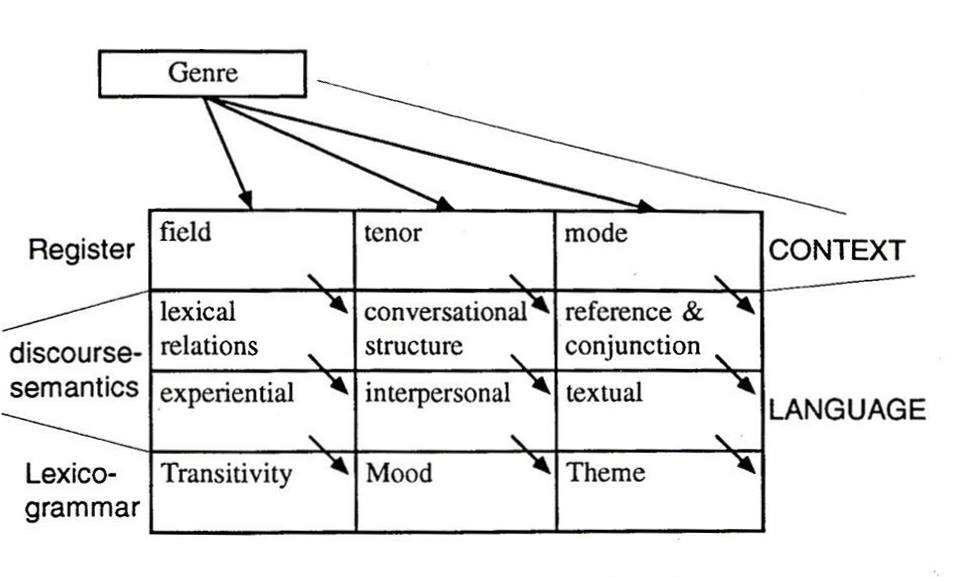
\includegraphics[width=0.65\textwidth]{../images/egginsfixed.jpg}}
\caption[Strata and metafunctions of language]{Strata and metafunctions of language (adapted from Eggins, 2004)}
\label{fig:eggins}
\end{figure}

\subsection{Affordances of \glsfmtshort{SFL} for researching an \glsfmtshort{OSG}}

\gls{SFL} has been applied to a diverse array of research areas including first and second language acquisition \cite{halliday1993towards,hasan_learning_1994}, language pedagogy \cite{halliday_towards_1993}, historical linguistics \cite{cummings2010introduction,martin_re/reading_2003} and (critical) discourse analysis \cite{hunston_systemic_2013,le_systematic_2009,martin_working_2003}. For the latter of these, \gls{SFL} is particularly useful, and has for this reason become one of the most popular grammars and theories of language for discursive research: as Halliday explains, at the most general level, \gls{SFL} is used `to understand the quality of texts: why a text means what it does, and why it is valued as it is' \parencite*[p.~xxx]{halliday_introduction:_2004}. In fact, from a systemic\hyp{}functional perspective, the use of a grammar is a prerequisite for all discourse analytic research. In Halliday's words,

\begin{quote}\small\singlespacing
it is sometimes assumed that discourse analysis, or `text linguistics' can be carried on without grammar---or even that it is somehow an alternative to grammar. But this is an illusion. A discourse analysis that is not based on grammar is not an analysis at all, but simply a running commentary on a text \parencite*[p.~xvii]{halliday_introduction:_2004}).
\end{quote}
%
%todo: reword again?
As a result of this conviction, the organisation and metalanguage of \gls{SFL} has in part been designed with text analysis in mind.

%todo: add zappavigna , hunston, cmc contexts...

The overall utility of \gls{SFL} for analysis of an \gls{OSG} may be divided into three main factors: the treatment of language as constitutive of text, the notion of language as a meaning\hyp{}making resource, and the division of interpersonal and experiential metafunctions within a grammar. These three factors are outlined below.

\subsubsection{Language as constitutive of context} \label{sect:context-in-text}

Though context is an increasingly central concern within many branches of linguistics, \gls{SFL} is notable for the extent to which its theory of context has been articulated and empirically applied \cite{widdowson_text_2008}. Halliday explains that in \gls{SFL}, context and text are in fact seen as `aspects of the same process', and that any sample of language use thus in fact `goes beyond what is said and written: it includes [...] the total environment in which a text unfolds' \parencite*[p.~5]{halliday_language_1989}. Therefore, \gls{SFL} treats language as constitutive of, rather than simply bound to, its context. As context can often be accurately deduced from text alone, and as context can be used to predict appropriate kinds of texts, some \gls{SFL} theorists contend that \emph{context is in text} \cite[e.g.][p.~7]{eggins_introduction_2004}. Context and language thus together construct both a reality and roles for people within it \cite{veel_learning_1997}.

This notion of language as simultaneously constructing and responding to the demands of contexts of situation has often formed an implicit theoretical assumption in online community and \gls{OSG} research: many works reviewed in the previous chapter tacitly take the perspective that language \emph{must} be responsible for the development of distinct cultures in online groups, as language is often the sole semiotic system available to group members \cite{thorne_computer-mediated_2008}.

%The absence of research explicitly drawing upon \gls{SFL} for online discourse socialisation research is thus striking.

\subsubsection{Language as a meaning-making resource}

The \glslink{SFL}{systemic\hyp{}functional} approach foremost involves an understanding of language as a semiotic system strategically drawn upon by language users as a meaning\hyp{}making resource---`how people use language with each other in accomplishing everyday social life' \cite[p.~2]{eggins_introduction_2004}. The orientation of the theory toward function and meaning\hyp{}making may be contrasted with phrase structure grammars, which typically do not attempt to account for meaning or pragmatics, and which are not grounded in analysis of realised linguistic patterns, but instead seek to provide rules that conform to speakers' intuitions regarding what is grammatically possible to say \cite{martin_english_1992}. \gls{SFL}, in contrast, understands language as \emph{purposive}: its use is motivated by purposes that may or may not be transparent or tangible. This is an appropriate theoretical stance for investigations of linguistic choices in an online community, because all communities are inherently social, and because in text\hyp{}based \gls{CMC} language is the main resource upon which members can draw to achieve their respective goals.

%\paragraph{Quantifiability of linguistic features}
%Halliday explains that it is possible to evaluate texts by counting the frequencies of relevant phenomena...
%Halliday remarks on the potential usefulness of very large datasets \parencite*{halliday_language_1992}
%This is amenable to the corpus-based approach taken here.

\subsubsection{Interpersonal and experiential functions of language}

%todo: add a ref to harvey so it doesn't seem like a fudge
From a systemic perspective, the simultaneous provision of health information and social support within \glspl{OSG} is realised by \glslink{member}{users} attending simultaneously to two metafunctions of language: an interpersonal dimension, responsible for negotiating role relationships, and an experiential dimension, responsible for communicating propositions about the world. This is the most useful affordance of \gls{SFL} for investigation of \glspl{OSG}, because the division of types of meaning is central to the reason for the community's existence: if the social element were not desired, \glslink{member}{users} would likely be content to simply read from static pages; if experiential content were not desired, health communities and the threads within them would not need to be organised by topic and subtopic. The interest in the phenomenon of \emph{advice} noted in Section \ref{sect:advice} would likewise stand to benefit from clearer delineation of the relationship between social roles and ideational content, each of which occupies a distinct, but overlapping space within acts of advising or directing others to act. Such a delineation would likely not be unwelcome. Early conceptualisations of the process of social support bear striking resemblance to the systemic model of interpersonal meaning: \textcite[p.~11]{shumaker1984toward} remind us, for instance, that social support is foremost `an exchange of resources between two individuals'.

\subsubsection{\glsfmtshort{SFL} and corpus linguistics}

In systemic\hyp{}functional terms, the \gls{corpus} is a large collection of instances of language use. These instances are typically organised by register, or by register dimensions. Automated counting of patterns in these instances is one possible way to uncover the grammar---that is, the patterns that generalise across the instances. A particular benefit of \gls{CL} approaches is that they make it possible to sketch out the probabilities of certain choices in certain contexts. At the same time, \gls{CL} approaches can test key tenets of \gls{SFL} theory \cite{honnibal_creating_2007}. \textcite{clarke_patterns_2012}, for example, uses a corpus-based approach to test the context metafunction hookup hypothesis---that is, the connection between language and context.

\gls{CL} and \gls{SFL} also share a number of underlying similarities. Most obviously, both are concerned with analysis of natural language, and both share a conceptualisation of \emph{register} as playing a significant role in shaping the \glslink{lexicogrammar}{lexicogrammatical} patterns to be found within texts \cite{hunston_systemic_2013}. Another key point of convergence between \gls{SFL} and \gls{CL} is in the treatment (explicit in \gls{SFL}, generally implicit in \gls{CL}) of context as being \emph{contained within} instantiated texts---`context is in text', rather than around it \cite{eggins_introduction_2004}. Systemicists evidence this assertion through the fact that we can often accurately deduce the overall functions, purposes and genres of highly decontextualised fragments of texts: \emph{Submissions must contain 8--10 references} can be quickly identified as part of a set of instructions for the submission of academic work, based purely on its lexical (submissions, references) and grammatical (nominalisation, modalisation, etc.) properties. In the same way, Halliday conceptualises \glslink{lexicogrammar}{lexicogrammatical} features of texts as probabilistically determined by their context. That is to say, a given constellation of interpersonal, experiential and textual variables (e.g. the writing of a professor to undergraduates in a written course overview) will likely contain the kinds of \glslink{lexicogrammar}{lexicogrammatical} features described in the example above \cite{halliday_corpus_1991}. This conceptualisation is of great benefit to corpus linguists interested in discourse analysis: given that \gls{CL} methods inherently involve the stripping of contextual information from natural language, and that analysis of contextualised language is preferred within the discourse analytic tradition, the recognition of context within \gls{lexicogrammar} allows \gls{CL} practitioners to address the common claim  \cite[e.g.][]{virtanen_discourse_2009} that \glslink{CL}{corpus} and discourse linguistic approaches, having very different orientations toward context, are difficult to reconcile.

\subsection{Overview of relevant elements of \glsfmtshort{SFG}}

%ntodo: sfl glossary weirdness
The core of \gls{SFL} is its grammar, known as the \glsxtrfull{SFG}, which is organised along the three axes discussed above. In this section, I describe the parts of the \gls{SFG} that are most relevant to the case study. The major references for this section include \citeauthor{halliday_introduction_2004} 2004, \citeauthor{matthiessen_lexicogrammatical_1995} 1995, and \citeauthor{eggins_introduction_2004} 2004.

\subsubsection{Register}

%todo: clean up, no repeating
Register occupies the level of abstraction above \glspl{discourse-semantic}, where language interfaces with a context of situation. The total content of each metafunction (interpersonal, experiential and textual) respectively corresponds to the three register variables of \emph{Tenor}, \emph{Field} and \emph{Mode} \cite{halliday_language_1989}. Halliday provides a minimal definition of each component:

\begin{enumerate}
\item  `The \sctext{Field of discourse} refers \emph{to what is happening}'
\item `The \sctext{Tenor of discourse} refers to \emph{who is taking part}'
\item `The \sctext{Mode of discourse} refers to \emph{what part the language is playing}' \parencite*[p.~12]{halliday_language_1989}
\end{enumerate}
%
In \gls{SFL}, doing register analysis can refer either to creating qualitative descriptions of the Field, Tenor and \gls{Mode} of a text (or collection of related texts), or to the process of generating quantitative, corpus\hyp{}based models of these features \cite{lukin2011halliday,matthiessen_modeling_2015}. Qualitative descriptions are intended to provide `[an interpretation of] the social context of a text, the environment in which meanings are being exchanged' \cite[p.~12]{halliday_language_1989}. Quantitatively, the internal dimensions of a single register can be modelled by counting relevant \glslink{lexicogrammar}{lexicogrammatical} features. The distribution of Process Types and the participants engaged in them, for instance, can be used to determine how speakers construe the world around them; \sctext{Mood} features can be analysed in order to see how speakers position themselves with respect to others (see below). 

Using a cartographic metaphor, \textcite{matthiessen_modeling_2015,Matthiessen2015} calls for further work within functional linguistics that models the internal dimensions of registers, and then situates these models within a cluster of related registers (presented later as Figure \ref{fig:pie-of-fortune}). By comparing these distributions to those found in other registers, registers can be arranged as a landscape, either along the axis of stratification or instantiation. The ultimate, perhaps distant goal, is to synthesise information about individual registers, in order to form a description of the meaning potential of a language, realising the notion of language as `an assembly or assemblage of registers' \parencite*[p.~44]{matthiessen_modeling_2015}. 

\textcite{matthiessen_applying_2013} has also applied register analysis to the domain of healthcare. Within the \gls{consumercentred} paradigm, this means focussing on individual healthcare consumers' health journeys, rather than on, for example, how consumers move through a given hospital or clinic in general. These healthcare journeys, Matthiessen explains, consist of sequence of encounters with formal and informal healthcare institutions. Each encounter presents a registerial configuration of topic, interactants and media: we may speak with a doctor in a busy clinic about our symptoms, or to a mental health practitioner about our personal relationships in an hour\hyp{}long consultation; we may phone an insurance carrier to clarify an issue about coverage, and write to a family member on Facebook about what we have learned. The case study of this thesis, centred on the registerial environment of an \gls{OSG}, has yet to be described within \gls{SFL} or \gls{HC} literature. The registerial description provided in Chapter \ref{chap:discuss-bp} is therefore intended to facilitate the addition of this register to the current body of knowledge and descriptions of the kinds of registers that may be encountered within consumers' journeys beyond the clinic.

%These meanings are realisations within the \sctext{Mood} and \sctext{Transitivity} choices that \gls{Forum} \glspl{member} make in their \glspl{post}. The two metafunctions and their implicated grammatical systems are described below. Chapters \ref{chap:researchdesign}--\ref{chap:experiential} combine to provide a quantitative model of the register of the \glslink{Forum}{Bipolar Forum}. Chapter \ref{chap:discuss-bp} presents a qualitative summary of Field, Tenor and Mode.

\subsubsection{Interpersonal meanings, MOOD and MODALITY} \label{sect:mood}

The Tenor variable of register is realised by interpersonal meanings. In turn, these meanings are made via the \sctext{Mood} and \sctext{Modality} systems of the \gls{lexicogrammar}. The interpersonal metafunction is responsible for negotiating role\hyp{}relationships with other speakers. It thus facilitates a constant \emph{exchange} of material and semiotic commodities; it is used to \emph{enact}, and to \emph{interact}.

\paragraph{Speech Function and Mood\slash Indicative Type}

In the \gls{SFG}, at the broadest level, utterances involve two potential \emph{speech roles}: \emph{giving} and \emph{demanding}. Within either speech role, two types of commodities may potentially be given or demanded: \emph{information}, or \emph{goods and services}. This leads to four main \emph{speech functions}, each of which is congruently realised by a different \sctext{Mood Type}. Information is given via statements, which are realised with declarative Mood. Information can be demanded via questions, congruently realised with the interrogative Mood. Goods and services are given via modalised declaratives. Demands for these non\hyp{}semiotic commodities are made via commands, which are realised with (non-indicative) imperative Mood. These intrastratal relationships are summarised in Table \ref{tab:roles}.

\begin{table}[htb]
\centering\small
\begin{tabular}{lll}

\toprule
\textbf{} & \textbf{Information} & \textbf{Goods and services} \\ 
\midrule
\textbf{Giving}   & statement $\rightarrow$ declarative    & offer $\rightarrow$ modalised interrogative     \\ 
\textbf{Demanding}   & question $\rightarrow$ interrogative & command $\rightarrow$ imperative    \\
\bottomrule
\end{tabular}
\caption[Mood Type and Speech Function]{Speech roles, commodities, speech functions and congruent \sctext{Mood Types} in SFL}
\label{tab:roles}
\end{table}   

\paragraph{Grammar of the \sctext{Mood} system} \label{sect:mood-grammar}

Each indicative clause contains a \emph{Mood Block}, comprised of a \emph{Subject} and \emph{Finite}. Optionally, clauses may also contain a \emph{Residue Block}, which can include a \emph{Predicator}, a \emph{Complement}, and\slash or one or more \emph{Adjuncts}. As non-indicatives, imperatives are comprised entirely of the Residue Block. In the case of declaratives, to determine which element is the Mood Block, a reverse-polarity tag can be added to the end of the declarative:

\begin{quote}
Geoff had difficulty with the task, \emph{didn't he?}
\end{quote}
%
Whatever is referenced by the pronoun in the tag is the Subject component of the Mood Block. The Finite is the first verb or modal in the verbal group that follows. It too is duplicated in a tag question in the case of \emph{be}, \emph{have} or a modal Finite; it is replaced by \emph{do} in other cases. The \emph{Polarity}, which is often unmarked when positive, is the opposite of the polarity in the tag. These elements together form the Mood Block. What remains in the clause is the Residue.

Residue also has component parts: the \emph{Predicator} is the part of the verbal group that carries a sense of the actual process undertaken. When a clause has only a single-word verbal group, it functions as both Finite and Predicator. If there is secondary tense information such as a progressive element, it is realised in the Predicator \cite{halliday_introduction_2004}. Residue may also contain a \emph{Complement}. The Complement is what becomes Subject if the clause is passivised. Finally, \emph{Adjuncts} are elements of the Residue that contribute non-essential information. Generally realised by adverbial or prepositional groups, Adjuncts cannot be turned into Subjects through passivisation.

Adjuncts may be \emph{circumstantial} (experiential), \emph{modal} (interpersonal), or \emph{textual} (thematic). Circumstantial adjuncts are those that add information concerning cause, time, matter or agent (discussed in the next section). Modal adjuncts\endnote{A fuller account of the differences and tests needed to differentiate mood adjuncts has been provided by \textcite{eggins_introduction_2004}.}~provide information concerning mood or polarity, or comment (the speaker's assessment of the clause) or vocative (naming speakers for addressal, turn\hyp{}taking, etc.). Finally, thematic adjuncts may have the role of facilitating conjunction or continuity with other clauses.

Importantly, some Mood Adjuncts are realised through \emph{grammatical metaphor}---that is, when what is congruently expressed through one rank or component is expressed through another.
%
\begin{multicols}{2}
\begin{quote}
\sctext{Grammatical metaphor}

\emph{I think} he came back.
\end{quote}

\begin{quote}
\sctext{Congruent form}

= \emph{Perhaps} he came back.
\end{quote}
\end{multicols}
%
\noindent \emph{I think}, for example, involves a grammatical metaphor---in this case, upward rank shift, where meaning typically realised by a word (in this case, a modal operator or Mood adjunct) is realised by an entire clause \cite{halliday_concept_1966,taverniers_systemic-functional_2002}. The fact that \emph{I think} is functioning as a constituent, rather than as an independent clause, can be ascertained by the tag question test: in the examples below, we can see that \emph{he} and \emph{'s} are typically the Subject and Finite within the Mood adjunct:

\begin{multicols}{2}
\begin{quote}
I think he's OK, \emph{isn't he?}
\end{quote}

\begin{quote}
*? I think he's OK, don't I?
\end{quote}
\end{multicols}
%
\noindent Because \emph{I think} is not functioning as an independent clause, it `play[s] no part in the structure of the interaction' \cite[p.~162]{halliday_introduction_2004}.

Differences in Indicative\slash Mood Type are realised by different configurations of the Subject, Finite and Predicator. For polar interrogatives, the Finite and Subject simply switch places. Aside from copula constructions, whenever the Finite and Predicator are realised with the same word, the operator \emph{do} must be inserted as the Finite for interrogatives:

\begin{multicols}{2}
\begin{quote}
\emph{Have you gone this week?}
\end{quote}
\begin{quote}
\emph{Do you know the way?}
\end{quote}
\end{multicols}
%
\noindent For WH\hyp{}Interrogatives, `the WH\hyp{}element is always conflated (mapped onto, fused with) another element of clause structure' \cite[p.~175]{eggins_introduction_2004}. It may potentially be mapped onto Subjects, Complements or circumstantial Adjuncts. Whichever element it is mapped onto is the same element needed in a minimally satisfactory reply:


\begin{multicols}{2}
\begin{quote}
\emph{Who moved the table?}

\emph{When did he do it?}
\end{quote}
\begin{quote}
\emph{Mahsa.}

\emph{An hour or two ago.}
\end{quote}
\end{multicols}

%
\noindent The Mood structure of basic imperatives involves removing the Mood element altogether:

\begin{multicols}{2}
\begin{quote}
\sctext{Interrogative\slash question}

\emph{Have you been taking} your meds?
\end{quote}

\begin{quote}
\sctext{Imperative\slash command}

\emph{Take} your meds.
\end{quote}
\end{multicols}

%\begin{multicols}{2}
%\begin{quote}
%\emph{Go to where the pepper grows!}
%\end{quote}
%\begin{quote}
%\emph{Let him speak!}
%\end{quote}
%\end{multicols}

% Imperatives involving \emph{let} are treated unusually by SFG \cite{huddleston_constituency_1988}. \emph{Let} is seen as `enabling the expression of the subject', and is thus treated within the subject component of the Mood Block:\endnote{Other varieties of English imperative such as \emph{`Don't you take my copy of the Bostonians'} are analysed in \textcite[pp.~184--5]{eggins_introduction_2004}}~

\paragraph{Metaphorical realisations of Speech Function}

The correspondence between interpersonal semantics and \sctext{Mood} choices is not always one\hyp{}to\hyp{}one. In situations where interactants are of a relatively equal social status, incongruence between Mood Type and Speech Function emerges as a politeness or hedging strategy. In particular, commands may be realised through alternative Mood Type choices (Table \ref{tab:gram_met_mood}). The most appropriate and\slash or likely choice is dependent on the overall Tenor of an interaction, and on who is speaking. In unequal relationships, the higher status participant tends toward congruent, imperative realisations of commands, while the lower status participant opts for incongruence (\emph{Would you be so kind as to ...}).

\begin{table}[htb]
    \begin{tabular}{ll}
    \toprule
    Mood type & Realisation \\
     \midrule
    Command & \emph{Go back on the meds.} \\
    Declarative & \emph{I think you should go back on the meds} \\
    Interrogative &  \emph{Why don't you go back on the meds?} \\
    Mod. declarative & \emph{I would go back on the meds (if I were you).} \\
    \bottomrule
    \end{tabular}
\caption{Grammatical metaphor as politeness strategy}
\label{tab:gram_met_mood}
\end{table}
%
As reviewed in the previous chapter, the relationship between congruence of \sctext{Mood Type} selection and the role relationships of speakers in an interaction has already been noted in the context of advice provision by \textcite[see Section \ref{sect:advice}]{decapua_`if_1995}. Accordingly, in an \gls{OSG}, we can expect that the role-relationship disparity between long and short term users may manifest linguistically in imperative commands being issued by veterans, with the proportion of advice issued via imperatives increasing with the membership length of the veteran member. Notably, this kind of incongruence poses a challenge for corpus\hyp{}based methods.

%\begin{enumerate}
%    \item Go back on the meds.
%    \item I think you should go back on the meds % this is modulated! :(
%    \item Why don't you go back on the meds?
%    \item I would go back on the meds (if I were you).
%\end{enumerate}

\paragraph{MODALITY} \label{sect:modality}

\sctext{Modality} is a key resource within the interpersonal exchange. It is realised within Mood structure in two ways: \emph{modalisation} and \emph{modulation} \cite[p.~179]{eggins_introduction_2004}. Functionally, modalisation is when a speaker makes meaning related to the \emph{probability} or the \emph{usuality} of an event: as Eggins explains, `modalisation is the expression of the speaker's attitude towards what s\slash he's saying' \parencite*[p.~180]{eggins_introduction_2004}. Grammatically, modalisation may be realised through Mood adjuncts (as explained earlier), a modal operator, or both at the same time. In every case, the modal elements are gradable. 

\setlength{\columnsep}{-5mm}
\begin{multicols}{3}\raggedright{
\begin{quote}
\sctext{Mood adjunct}

\singlespacing{She \emph{certainly} knew the text well.}
\end{quote}
\begin{quote}
\sctext{Modal operator}

\singlespacing{Power \emph{may} have been restored.}
\end{quote}
\begin{quote}
\sctext{Both together}

\singlespacing{I \emph{could sometimes} win.}
\end{quote}
}
\end{multicols}
%
% does this fit?
Modals may therefore be expected to appear in a number of situations within an \gls{OSG}, including marking of hesitation by newcomers \cite{vayreda_social_2009,weber_missed_2011}, and in veterans' polite sharing of information and potential actions.

\paragraph{POLARITY}

\sctext{Polarity} is the binary opposition between positive and negative. In \gls{SFL}, \sctext{Polarity} is primarily considered an interpersonal feature, since in contracted forms it becomes attached to the Finite \cite[p.~143]{halliday_introduction_2004}. It represents the two poles of certainty, with modalisation and modulation construing various levels of certainty and uncertainty in between. \textcite{halliday_introduction_2004} provide corpus evidence that clausal \sctext{polarity} is positive in 90 per cent of cases; negative polarity, they claim, is always the marked variant. Its meaning, however, is highly dependent on the content of the clauses to which it responds, functioning as affirmation or denial of the validity of the previous proposition or proposal. As such, it is difficult to track using existing corpus methods. This difficulty is exacerbated in the case study, which treats individual \glspl{post}, rather than \glspl{thread}, as the unit of analysis. Though the proportion of responses that affirm or deny the content of the previous clause would no doubt shed light on the extent to which exchanges are harmonious or contentious, this is unassessable without shifting the unit of analysis to the \gls{thread}, which would in turn make difficult the analysis of how language use changes over the course of membership. \sctext{Polarity} is therefore accounted for in the case study mostly for the sake of completeness of the overall analysis of the \sctext{Mood} system, and the interpersonal meanings the system is responsible for realising.

\subsubsection{Experiential meanings and the system of TRANSITIVITY} \label{sect:trans}

As explained earlier, clauses in \gls{SFL} are multifunctional units. At the same time as interpersonal relationships are enacted and negotiated through choices of \sctext{Mood} and \sctext{Modality}, experiential meanings are being expressed via the \sctext{Transitivity} system. Through this metafunction, speakers make \emph{representations} of inner and outer states, and of Things in the world and Events that they are involved in. In each clause, language users are \emph{construing} reality as change, which may affect or be affected by participants. Coherent clause complexes therefore represent sequences of change.

In \gls{SFL}, the \sctext{Transitivity} system can be analysed from two complementary perspectives: the \emph{transitive model}, in which processes are grouped according to types, and the \emph{ergative model}, where processes are bound to Mediums, through which they are made possible and therefore, without whom they cannot exist.

\paragraph{Transitive model}

In the transitive model, the clause is structured around a \emph{process}, indexed mostly by the Event---that is, the rightmost verb in the verbal group (and prepositions, for phrasal verbs):

\begin{multicols}{2}
\begin{quote}
\emph{i \textbf{consider} myself blessed having you guys}  % user-goody2shuz-863.txt.xml
\end{quote}
\begin{quote}
\emph{Oh \dots and her ex bf glen \textbf{broke up with} his gf} % user-goody2shuz-927.txt.xml
\end{quote}
\end{multicols}
%
\noindent This process must belong to a \emph{Process Type}. Process Types are distinguishable based foremost on lexis, but also on the grammar of the clause they head. Various syntactic and\slash or semantic tests can be used to disambiguate more difficult cases, though accurate Process Type identification by both human and machine has often proven challenging \cite{odonnell_survey_2009}. Each Process Type constrains the available configurations of participants (nominal groups) and circumstances (adverbial or prepositional phrases) in the clause. A summary of Process Types, identification tests and associated participant roles is given in Table \ref{tab:proctypeoverview}.

\begin{table}[htb]
\begin{tabularx}{\textwidth}{lXXXXX}

\toprule
\#~ & Process Type & Definition & Typical verbs & Identification test & Participants \\ \midrule
1.  & Material       & Doing tangible things         & \emph{kick, give, draw}   & \emph{What did x do?}        & Actor (goal) (range) (beneficiary) \\
2.  & Mental         & Thinking or feeling           & \emph{think, believe}    & \emph{What do you think, feel or know about y?}      & Senser, phenomenon        \\
3.  & Verbal         & Saying            & \emph{shout, yell, tell}    & \emph{What did x say?}       & Sayer, (receiver) (verbiage)   \\
4.  & Behavioural       & Psychological and \newline physiological behaviour & \emph{cough, smile, dream}  & Unmarked present tense has continuous sense            & Behaver (behaviour) (phenomenon)    \\
5.  & Existential       & `There' clauses            & \emph{be }      & Presence of non-locative \emph{there}    & Existent       \\
6a. & Relational \newline (ident.)   & Ways of being           & \emph{equal, mean, symbolise}  &  \emph{x is a member of the class a.}    & Attribute, carrier      \\
6b. & Relational \newline (attr.)   & Defining             & \emph{own}      & \emph{x serves to define the identity of y.}   & Cannot be passivised     \\
\bottomrule
\end{tabularx} 
\caption{Summary of Process Types}
\label{tab:proctypeoverview}
\end{table}

\FloatBarrier
\paragraph{Ergative model}

The ergative model of \sctext{Transitivity} conceptualises each clause as a quantum of change in the world, centred on a Process being carried out through a Medium. When the causer of the change is not mentioned, the result is a \emph{middle clause}---a construal of a \emph{happening}. In cases where the Medium does not bring about the process, an Agent may also be added (resulting in an \emph{effective clause}, or a \emph{doing}).

\begin{multicols}{2}
\begin{quote}
\small
\noindent \sctext{Medium + Process: Happening}

\noindent \emph{my dd is hitting manic mode and i think it 's time} 
\end{quote}

\begin{quote}
\small
\noindent \sctext{Agent + Process + Medium: Doing}

\noindent \emph{you hit a nerve and i felt the need to stand up for myself} % user-DB1973-9.txt.xml
\end{quote}
\end{multicols}
%
\noindent A critical difference between transitive and ergative models is that core participant roles can be disambiguated in the ergative model simply by checking for the existence of multiple nominal group arguments of a process: a two\hyp{}participant process will likely contain a \emph{Medium} and an \emph{Agent}, while a single\hyp{}participant process will be a Process\hyp{}Medium configuration. For corpus\slash computational linguistics, the ergative model therefore represents an ability to more easily identify agency, which can be expected to play an important role in the way participants in a Field of discourse are construed. That said, the transitive model is equally useful, highlighting experience of certain types of change by social actors. The two models are complementary; each is drawn upon in the analysis of \sctext{Transitivity} (Chapter \ref{chap:experiential}) according to its strengths.

%\begin{figure}[!ht]
%\centering
%\includegraphics[width=3in]{../../images/circ}
%\caption[System of circumstance]{System of circumstance (from Eggins, 2004)}
%\label{fig:circ}
%\end{figure}

%\paragraph{Theme: textual metafunction} \label{sect:theme}

%`The Theme is the element which serves as the point of departure for the message, it is that with which the clause is concerned' or again `the Theme is the starting-point for the message; it is what the clause is going to be about''. \cite[p.~158]{huddleston_constituency_1988}

%`In English, Halliday says, the Theme is identifiable as `that element which comes in initial position in the clause''' \cite[p.~158]{huddleston_constituency_1988}

% paragraph theme_textual_metafunction (end)



%todo: doesn't flow from previous
\subsubsection{Context of culture: genre and ideology} \label{sect:genre}

%todo: copy edit
While the case study of the thesis for the most part involves methods drawn from \gls{CL}, the analysis begins with a generic (i.e. genre\hyp{}based) interpretation of \glslink{post}{contributions} to the \gls{Forum}. For this reason, in this section, I provide a basic overview of a conceptualisation of genre that has emerged from the \glslink{SFL}{systemic-functional} school, and an associated method for performing genre analysis.\endnote{It is important to note that the interpretation of genre as a level of abstraction greater than that of register is a development rejected within the `Hallidayan' approach to SFL \cite{lukin2011halliday}. The genre analysis in Chapter \ref{chap:introdata} is performed because it elucidates in an intuitive way how Forum interactions may proceed in identifiable sequences, and how the probabilities for lexicogrammatical features are different within each sequence. Theoretical issues of language and context, such as where in the hierarchy of stratification the lexicogrammatical probabilities are set, and whether or not genre stages themselves reconfigure the probabilities, are not issues covered in this thesis.}

%there are \cite[e.g.][]{fawcett_theory_2000}

In contrast to the context of situation, which concerns the environment in which a given text is produced, the context of culture refers to the broader conditions common to texts. Culture is the highest level of abstraction in \gls{SFL}---all other meaning systems exist within and belong to cultures \cite{halliday_language_1989}. Thus, the context of culture is the semiotic potential of the totality of sign systems. 

The best\hyp{}articulated component of the context of culture is the notion of \emph{genre}---that is, `recurrent configuration[s] of meaning, phased in discourse as a staged, goal-oriented social process' \cite[p.~9]{martin_genre-based_2013}. Genres ultimately derive their meaning from their instantiation within a given culture \cite[p.~99]{halliday_language_1989}. Though genre and register alike are realised by the contextual variables of Field, Tenor and Mode, genre theory emphasises the social purpose of the activity being undertaken in the text \cite{christie_genre_2005,martin_english_1992}. Thus, genres may be characterised as constellations of Field, Tenor and Mode that are culturally recognised as performing social functions \cite{eggins_introduction_2004}. It is also important to bear in mind when considering genre that individual genres are not necessarily distinct: \emph{macro-genres} may contain \emph{micro-genres}: the macro-genre of the \emph{essay}, for instance may draw on micro-genres of \emph{expositions}, \emph{discussions} and \emph{evaluative accounts}.

\textcite{eggins_analysing_2004} provide simplified, actionable parameters for performing systemic\hyp{}functional genre analysis. The six steps are outlined below.

\paragraph{Recognising a generic text}

Given that genres are culturally recognised by their very nature, simple reading of texts by those fluent in the relevant culture may be enough to identify the existence of a genre. For analysts and interactants alike, genres are recognised when texts appear to `move through predictable stages' \parencite*[p.~213]{eggins_analysing_2004}. \textcite{eggins_introduction_2004} argues that the existence of a word for the kind of behaviour seen in the text (i.e. \emph{purchasing}, \emph{commentating}, \emph{gossiping}) may at the very least be a clue that a potentially definable genre exists.

\paragraph{Defining the social purpose of the generic text}

This step involves clarifying the overall function(s) of a genre with as much specificity as possible---rather than `telling a story', sub\hyp{}categorisations such as `anecdote' or `exemplum' are more useful, given the existence of micro- and macro\hyp{}genres. More theoretically, this task also involves developing an understanding of how the genre constructs a social reality: by virtue of their existence alone, recognisable genre stages may provide insight into social practices and culturally accepted attitudes and values. 

\paragraph{Identifying and differentiating stages within a genre}

After breaking down the text into clauses as with \glslink{lexicogrammar}{lexicogrammatical} analysis, groups of these clauses must be divided by their role within the text. These roles should be functionally, rather than formally defined: \emph{Abstract} or \emph{Resolution} is superior to \emph{Beginning} or \emph{Chapter Three} because the latter are not genre specific. By convention, each of these functions should then in turn be described in prose.

\paragraph{Specifying obligatory, optional and recursive stages}

Stages may be obligatory, optional or recursive. Obligatory elements are considered to be defining features, and in some cases may be unique to the genre under investigation. Optional stages, on the other hand, are likely to be present in other genres. \textcite{halliday_language_1989} remind us that optional stages do not occur randomly: in the \emph{buying and selling genre}, the number of customers in the store or the size of the line may affect whether or not a \emph{greeting} or \emph{sale initiation} takes place. Both optional and obligatory stages may be recursive, as in the case of the buying and selling genre, in which \emph{sale request}, \emph{sale enquiry}, \emph{sale compliance} and \emph{sale} may go through limitless iterations \cite[p.~61]{halliday_language_1989}.

\paragraph{Devising a structural formula}

The next task is to represent the genre structure. By convention, each genre stage is delineated by a caret (~$\hat{}$~). Optional stages are bracketed. Recursive stages are square-bracketed, with brackets followed by  \textsuperscript{n}.

A number of notion schemes for representing the relationship between genre stages have been proposed, and many have undergone revisions in order to be easier to render on a computer \cite{eggins_introduction_2004}. Problematic is that many \cite[e.g. those in][]{halliday_language_1989} are esoteric, and lagging behind the representational schemes of other grammars in terms of readability (Hovy, 1996). In fact, the development and use of unique means of expressing optionality and recursion is perhaps superfluous and ultimately unhelpful, given that comparatively well\hyp{}known systems such as \emph{regular expressions} could potentially represent generic structure in a format familiar to at least some non\hyp{}\gls{SFL} practitioners. 

A particularly important addition to structural representation of genre is Hasan's \parencite*{hasan_structure_1985} notion of \emph{generic structure potential}: that is, a maximally expanded representation of genre staging that exhausts all possibilities for additional optional stages and recursion.\endnote{It is important to distinguish generic structure potential from \emph{genre potential}---that is, `all the linguistically-achieved activity types recognised as meaningful (i.e. appropriate) in a given culture' \cite[p.~35]{eggins_introduction_2004}. In practice, this translates to every possible configuration of Field, Tenor and Mode.}

\paragraph{Analysing the semantic and \glslink{lexicogrammar}{lexicogrammatical} features for each stage of a genre}

As Hasan explains,

\begin{quote}\singlespacing\small
a text has many modes of existence and so it can be analysed at many different levels, with each contributing to our understanding of the phenomena involved \parencite*[p.~116]{halliday_language_1989}.
\end{quote}
%
\noindent Thus, relevant parts of \gls{SFG} may be operationalised in order to investigate the phenomena of interest: a researcher interested in power dynamics within a text, for example, would likely perform an analysis of features of the \sctext{Mood} system, as these are responsible for the management of role\hyp{}relationships between interactants. Simultaneously, this analysis provides a justification of the treatment of the text as instantiating a genre and of the clause complexes as instantiating generic stages. \textcite{eggins_analysing_2004} note that since \gls{lexicogrammar} can provide hints as to genre staging, this step of the analysis may render it necessary to reconsider the previous delineation of stages.

Genre may influence the \gls{lexicogrammar} of texts in two ways. First, as genres are configurations of register variables, texts within genres must necessarily conform at the level of lexicogrammar. In this way, a genre such as \emph{sports commentary} is likely to bring about language which experientially positions players, teams, umpires and coaches as the main participants. Second, different genre \emph{stages} may influence \glslink{lexicogrammar}{lexicogrammatical} decisions. The \emph{evaluation} stage within the \emph{storytelling} macro\hyp{}genre, for example, is likely to opt for a declarative Mood, while experientially, it can be assumed that mental and relational Process Types may occur.

\paragraph{Ideology in SFL}

Ideology has a complex history within \gls{SFL}, originally conceptualised as the most abstract analysable stratum of text\slash context, as the overarching determinant of the context of culture \cite{eggins_introduction_2004}. Later work, however, often refrains from accounting for ideology \cite[e.g.][]{matthiessen_key_2010}, or disavows its existence as a distinct stratum within the hierarchy of stratification \cite[e.g.]{martin_genre_2006}. Regardless of its exact status within \gls{SFL}, ideology is commonly discussed in the contexts of both \glspl{OSG} and socialisation, and, accordingly, is in need of a brief description here.

One way of conceptualising ideology is `from above'. As \textcite{banks2009ideology} explains, two texts with very similar Field, Tenor and Mode can nonetheless mean very different things: politicians with opposing views, for instance, may give speeches within more or less identical registers, while ultimately expressing different sets of values. Ideology can also be conceptualised `from below': ideological values may be found within lexicogrammatical and semantic patterns that are common within a text, but that are rarely subject to negotiation, controversy or debate by the interactants. Experientially, while `Field of discourse' refers to what is being directly spoken about in a text, ideology refers more to the taken\hyp{}for\hyp{}granted assumptions about these things and events. For example, while there is a great deal of argument about the efficacy of some kinds of alternative medicine in many \glspl{OSG}, there is generally much less debate about the value of treatment itself: treatment can lead toward health, and is almost always worth undertaking. Some ideological values in these communities, therefore, may be that \emph{that illness requires treatment}, because \emph{treatment can make you healthy again}. The controversy surrounding pro\hyp{}anorexia \glspl{OSG} \cite[see e.g.][]{chancellor_recovery_2016} stems from the fact that these communities advocate challenging widely held ideological values about health, weight, illness and treatment.

In this thesis, without taking a particular stance on the role of ideology within \gls{SFL}, the term can still be operationalised in the case study as a way of referring to the more or less unargued or inarguable components of discourse within the \gls{Forum}. It is important to bear in mind, therefore, that ideology may or may not be substantively different from \glspl{discourse-semantic} or register; rather, here, it is simply a way of thinking about what the language users in texts take for granted or consider common\hyp{}sense.

\subsection{Criticism of \glsfmtshort{SFL}}

Both the overall orientation of \gls{SFL} and its grammar have received a number of criticisms that deserve to be addressed. \textcite{van_dijk_text_2004}, for example, has taken issue with three main dimensions of \gls{SFL} as a linguistic theory in general. First and most broadly, he notes that its sheer density creates difficulty when a researcher seeks to use only relevant sections of the theory:  `not only are the terms (Field, Tenor, Mode) hardly transparent, as to their intended meanings, but also the usual---informal---descriptions of their meanings are barely enlightening' \parencite*[p.~341]{van_dijk_text_2004}. Second, he characterises \gls{SFL} as lacking sufficient engagement with potentially useful interdisciplinary perspectives: `there is very little inspiration from the many other approaches to context in linguistics and especially in anthropology, sociology or social psychology, at least in the analysis of the context' \parencite*[p.~342]{van_dijk_text_2004}. Finally, he points out that \gls{SFL} has avoided engaging with cognitive accounts of language, and therefore can have little to say about the reality of the meaning\hyp{}making process for speakers themselves.

%todo: copy edit
Indeed, each of the three points is in some sense valid. \gls{SFL} is terminologically dense---a necessary evil, according to Halliday's preface to his \emph{Introduction to Functional Grammar}, when formulating a theoretical account of something as complex as a human language.  Van Dijk's second point, regarding a lack of dialogue between \gls{SFL} is also accurate. At a terminological level, for example, key terms in \gls{SFL} such as \emph{Tenor} have been coined in order to avoid ambiguity---a more natural term might be \emph{tone}, but this term also has a phonological meaning. The claim that \gls{SFL} engages little with related traditions at both the level of terminological and beyond is not a baseless one, however: as a second example, the $650+$ page \emph{Introduction to Functional Grammar} does not once mention \emph{pragmatics}, though what is meant by pragmatics in related areas overlaps to a very significant extent with the systemic conceptualisation of interpersonal \glspl{discourse-semantic}.\endnote{Halliday has addressed a perceived lack of engagement with the field of pragmatics: Pragmatics, he argues `has always been simply the instantial end of the semantics. We don't need a separate discipline' \cite[p.~138]{thompson2001interview}.}

The third criticism, related to the lack of cognitive accounts, is the only one which has some bearing on the overall explanatory power of the theory. Here, Van Dijk is not alone in his criticism: \textcite{rohdenburg_cognitive_1996} has argued that the systemic account of preposition\slash object ordering in clauses with phrasal verbs (\emph{She put the fire out} vs. \emph{She put out the fire}) as being motivated by textual thematic demands (i.e. information structure, or givenness\slash newness) is only a partial account of the underlying motivations for speaker choices. Cognitive demands on addressees play an important role in choices between grammatical alternatives, with the likelihood of clause\hyp{}final preposition decreasing steadily as weight and length of the object grows \cite[c.f.][]{hawkins1992syntactic}. While a lack of engagement with cognition may have benefits for certain kinds of text analysis, as well as some computational tasks \cite{odonnell_[sys-func]_2014}, it is prudent to bear in mind that even if the systemic account may not in and of itself be incorrect, there is compelling evidence for its instead being in some respects only a partial account of how language works.

Others also critiqued the \gls{SFG}'s textual metafunction: \textcite{huddleston_constituency_1988} and \textcite{widdowson_text_2008} have problematised the notion of the \gls{Theme} as simply the first element in a clause, in cases where there are dummy subjects, for example. More generally speaking, Van Dijk has also further criticised what he sees as an attempt to force \glslink{lexicogrammar}{lexicogrammatical} \emph{conjunction} to line up with the register variable of \emph{Mode}. Perhaps this criticism is tacitly embraced by \textcite{eggins_analysing_2004}, who tend to advocate the use of terminology and concepts from \gls{CA}, rather than \gls{SFL}, for investigations of turn\hyp{}taking, overlap and the like. For these reasons, compounded simply by issues of scope, I have opted not to consider textual meanings in this thesis in any serious detail. This is perhaps unfortunate, as much could foreseeably be learned about \glspl{OSG} through analysis of the ways in which the take\hyp{}up of advice (for example) is realised in \gls{forum} \glspl{thread} (see Section \ref{sect:discuss-register} for a brief demonstration of the possible value of analysis of choices of Theme).

%Finally, it is worth noting that schisms exist within the overarching theory of \gls{SFL}, with the various factions tending to criticise



%\noindent In the context of \glspl{OSG}, the distinction between experiential, interpersonal and textual meanings allows the researcher to focus on components of the \gls{lexicogrammar} that realise the two major purposes of the community: health information provision can be investigated through experiential meanings and the Transitivity system, and social support and member role negotiation can be analysed by looking at how different Mood types (e.g. imperatives, declaratives, interrogatives) as well as Modality (communicating information regarding obligation, probability, usuality, etc). Accordingly, from a systemic functional perspective, we can predict that certain features of both Mood and Transitivity will be subject to change over the duration of membership. In terms of Mood and Modality, long term members would be more likely to provide information or suggest a course of action (congruently realised through declaratives and imperatives), while new members would request information (through interrogatives), and be very unlikely to issue commands. Furthermore, modalisation could be a resource for hedging claims to knowledge in newer members' posts, while veteran users may use modalisation to stress the obligations of less-knowledgeable members or the certainty of their own claims. In terms of experiential meanings, greater familiarity with community norms is likely to be observable through the instantiation of more elaborate taxonomies and configurations of participants and processes \cite{martin_english_1992}, with more nuanced distinctions being drawn over membership duration between more symptoms, medications, kinds of health professional, and so forth.%. Finally, the appraisal dimension of \gls{SFL} \cite[see][]{martin_language_2005} may also be subject to change throughout membership, as normative judgments of key participants and processes may evolve.

%In addition to face-to-face encounters, examples of anonymous self-dis- closure abound in today’s increasingly technological society. Crisis center hotlines provide the highly stressed caller with immediate feedback, which may simply involve listening, or may entail providing caring responses and referral services. Similarly, a growing number of radio talk shows provide participants with direct responses to their problems and listeners with vicarious information. The accelerated growth of home computers has provided an additional avenue for anonymous support. With the purchase of a modem, people can communicate with other “users”; programs have been developed to assist people in linking up with the resources of strangers (Van Gelder, 1983) \cite[p.~18]{shumaker1984toward}

%In \gls{SFL} and its expansions \cite[e.g.][]{martin_language_1984,christie_genre_2005}, culturally recognised constellations of these three variables are treated as \emph{genres}, within which other micro-genres may also be contained. In our case, the vast majority of texts under consideration are within the genre of newspaper article, with micro-genres such as sports-journalism, editorials, opinion articles and so on being differentiated by the appearance of different \glslink{lexicogrammar}{lexicogrammatical} choices within both mood (i.e. use of interrogative mood, modalisation to connote subjectivity/objectivity) and transitivity systems (what is being spoken about). 



%\subsection{\gls{SFL} and healthcare}

%\gls{SFL} practitioners have recently turned their attention to healthcare contexts. \textcite{matthiessen_applying_2013} demonstrates the potential use within the emerging paradigm of relationship centred healthcare, showing how we can map the patient journey through healthcare institutions.

%~\ \todo[inline,color=green!40]{\noindent More here on \gls{SFL} healthcare.}

%another one here that robyn uses

%\subsection{Relevant applications of \glsfmtshort{SFL}}

%\gls{SFL} has been applied for a broad range of purposes. Here, I focus on discourse analytic, \gls{CL} and computational applications.

%\todo[inline,color=green!40]{Redo this part!}

%\subsubsection{\glsfmtshort{SFL} and discourse analysis}

%The fact that \gls{SFL} provides a well-articulated means of connecting \gls{lexicogrammar} to meaning, discourse and register has made it a popular choice in (critical) discourse analysis.

%\todo[inline,color=green!40]{Summary here}


%\subsubsection{Computational \gls{SFL}}

%There have been many computational \gls{SFL} projects, focussing both on natural language generation and parsing. Focussing on parsing, early efforts encountered mixed results, with \cite{odonnell_uam_2005,odonnell_\gls{sfl}_2005} Some important work from this era remains copyright protected. For others, source-code has not been publicly released. More recently, Costetschi's approach has been to convert Stanford CoreNLP collapsed dependency annotations to a simplified systemic\hyp{}functional annotation through a rule-based system. Other work has centred on providing a web-based interface for manual tagging, from which automatic annotation can be learned (The Halliday Centre Tagger---see Wu, 2015).

% DANIEL with CCG

%Direct access to systemic features would indeed be preferable to the approach taken in this thesis, which is ad-hoc, wordlist based conversion of CoreNLP dependency annotation. A full treatment of issues with the approach is provided in Chapter 7.

% semantic parsing


%\subsection{Theoretical orientation}
%
%\gls{SFL} may be characterised as empirically driven and bound, probablistic, predictive and descriptive. A key notion in %\gls{SFL} is that functional definitions and distinctions extend as far as \glslink{lexicogrammar}{lexicogrammatical} distinctions can be reliably %made: distinctions between the different kinds of processes are evidenced by grammatical, rather than thematic %information. Alternative systems of Process Types (e.g. the Cardiff SFG) are intended more as a means of simplifying %the (at times very dense) distinctions made in the Sydney grammar.
%
%Contrastive distinctions between grammatical and ungrammatical constructions are thus of primary importance. %Probabalistic evidence (concerning words that are likely to collocate, or a trend toward passivisation of a certain %process, for example) is secondary. Probablistic parts of lexical or grammatical behaviour are inherently associated %with contrastive distinctions, but to widely varying extents. 
%
%Passivisation in signage, computer errors, etc. (\emph{Smoking is not allowed, Permission denied,} etc), is %predictable due to the fact that it is of little importance, or indeterminable, who would\slash could be the actor (%that is, the authority enforcing the rule) in the active version of the clause. Here, the phenomenon is closely tied %to the function of the message. On the other hand, though British and Raj collocate, and though in part this is due %to the close relationship between adjectival modifiers and nouns, the strength of the collocation is more to do with %historical circumstances: there have not been other kinds of Raj.
%
%Finally, it is worth noting that judgements based on native-speaker intuition alone are not meaningful for the %purposes of analysis, but are of course viable means of locating phenomena \emph{for} analysis.
%
%\gls{SFL} shares an unusual relationship with the prescriptive\slash descriptive debate. It is a profoundly functional %theory, but does indeed mark ungrammaticality in formal terms. This is a consequence of the goal of \gls{SFL} to provide a %description of grammatical systems. Ungrammatical utterances provide useful heuristics for L1 and L2 development, or %the particular functional aims of a speaker in a given interaction.
%
%\section{Interaffordances of the research areas}
%
%The combination of CMC, \gls{CL}s and \gls{SFL} presented here create some affordances. Some have been described %in existing literature; some are outlined for the first time here.
%
%\subsection{CMC and \gls{SFL}}
%
%\gls{SFL} has rarely been combined with studies of CMC.

% MACNAMARA 2010 cited as describing these IFG 2014 p. 42

%coffin?

%Focussing on a particular online support group stabilises certain systemic features. Most importantly, the contextual dimension of mode can be sketched fairly quickly, because users must use \emph{posts} to communicate. Though the site links to related communities (including, later in the evolution of the community, a dedicated space for friends and family of those living with bipolar disorder), these have an identical architecture. No other community-sanctioned spaces for further discussion appear to be provided.

%In the case of the bipolar forum, the most macro fields of discourse (bipolar disorder, mental health) are prescribed in the title and rules of the community. Off-topic information can be moved or deleted by administators at their discretion.


%\input{chapters/medical-nlp}

%todo: should this and the line below say 'literature review'?
\section[Chapter summary]{Summary: theories and methods for investigating online healthcare discourse}

The synthesis of literature presented in this and the previous chapter has involved four research domains:

\begin{enumerate}
	\item Computer mediated communication (CMC) as a Medium, and \glspl{forum} as a \gls{Mode}
	\item Healthcare communication (HC) as a Field
	\item Corpus linguistics (CL) as an approach for analysing digital linguistic data
	\item Systemic functional linguistics (SFL) as a framework for understanding language
\end{enumerate}
%
The argument made throughout the literature review is that by combining these areas, we can learn new things about online intra\hyp{}\gls{consumer} health discourse, as well as uncover new ways to learn things. Key claims from qualitative literature can be tested quantitatively with largely automatic \gls{CL} methods, and evidenced by translating observed discourses into their lexicogrammatical realisations. 

The next part of the thesis, which introduces the case study of a \gls{bipolar} \gls{OSG}, demonstrates the potentiality of combining \gls{CL} methods and \gls{SFL} theory for the analysis of \gls{CMC}. The systemic grammar and sophisticated corpus methods make possible nuanced kinds of corpus interrogation that differentiate interpersonal from experiential meaning\hyp{}making.

%In doing this, the divide between qualitative approaches to \gls{CMD} and quantitative approaches to improved healthcare through data mining can be bridged. Discourse can be brought into the purview of statistical approaches that have tended to focus on analysis of metadata; discourse\hyp{}oriented research can have more useful implications for real-world healthcare issues.


%\section{Chapter summary}

%In this chapter, I presented \gls{CL} as a possible approach to analysis of online health discourse, and \gls{SFL} as a means of understanding texts. From the synthesis of literature emerged the beginnings of a framework for repeatable, quantitative analysis of health discourse. In the next chapter, I operationalise the nascent framework through a case study of linguistic change in an \gls{OSG}.

%\bibliography{../references/libwin.bib}


%\part{Investigation}
%!TEX root = ../thesis.tex

\chapter{Case study design} \label{chap:researchdesign}

In the previous chapter, I reviewed relevant theory and methods for functional analysis of language use in \glspl{OSG}, centring on \gls{CL} as a potential approach and \gls{SFL} as a theory of language. This chapter introduces the case study of the thesis---a \gls{corpus}\hyp{}based analysis of an online \gls{bipolar} \glslink{OSG}{support group}. In the sections that follow, I describe the site selection and ethical considerations, data collection, and \gls{corpus} building processes. I then describe the analytical methods used in the investigation, and the development of \texttt{corpkit}, a \texttt{Python} module for building and interrogating \glspl{corpus}, and for editing and visualising interrogation results. Its core functionality and user interfaces are summarised. Justifications are provided for key choices throughout the chapter.

%There are currently dozens of bipolar disorder forums online. To locate the most suitable for analysis, I followed the method of \textcite{sillence_communicating_2012}. After locating eleven open-access bipolar disorder forums through search engine queries and exploring the basic infrastructure and content of each, \emph{Healthboards} was selected as the most suitable site for analysis. This choice was made for a number of reasons. First is its popularity: the \gls{Forum} is large and relatively active, having received over 66,000 \glspl{post} from thousands of unique users at the time of data collection. The presence of a number of users with thousands of \glspl{post} was also a prerequisite filled by the \gls{Forum}, as `veteran' members were required for the planned Investigation C. Second, the site has a global (English-speaking) focus: the presence of sizeable groups of users from most Anglophone countries was perceived to be a benefit. That said, the main nationality of Healthboards users is U.S. American, in part due to the site's use of U.S. American medication names, but also likely due to the existence of other bipolar disorder websites specifically designed for the UK (e.g. \emph{BipolarUK}), Australia (\emph{Beyond Blue, Blueboards}), etc.

%A third benefit of Healthboards is that the bipolar disorder forum is just one of many similarly structured boards for other health concerns. This allows potential future investigations to compare sub-forums, or analyse a group of sub-forums (e.g. all mental health forums) simultaneously. Fourth, Healthboards does not automatically delete old \glspl{post}, and has not undergone any renovations that have forced members to create new accounts. Thus, I had access to \glspl{post} dating back to the beginning of the message board, and could track individual users more accurately \cite{danescu-niculescu-mizil_no_2013}. Finally, at the time of data collection, Healthboards had no identifiable policy prohibiting web-crawling or re-use of content.

%\cite{danescu-niculescu-mizil_no_2013 In particular, it would be interesting to investigate how the patterns of linguistic change are affected by engagement in multiple communities, as well as how users that are members of multiple communities transfer norms and conventions between communities.

\section{Site description and selection}

The case study of this thesis is a \gls{corpus} comprised of 13 years of \glspl{post} to a once\hyp{}popular \gls{OSG} for those living with \gls{bipolar}---a mental disorder characterised by oscillation between elevated and depressed moods \cite{anderson_bipolar_2012}. The \gls{forum} has been online since 2001, with very little change to the interface or account system. As such, the \gls{Mode} dimension of the \gls{Forum} has stayed largely static, and many \glslink{member}{users} have participated using the same account details for a number of years. The \gls{Forum} is a part of a larger architecture of health-related \glslink{forum}{boards}, many of which were created at different points in time. \glslink{member}{Users'} accounts work site\hyp{}wide; as such, many of the contributors to the \glslink{forum}{Bipolar Forum} have also created \glspl{post} elsewhere. At the time of data collection (early 2014), the \glslink{forum}{Bipolar Forum} had over 5700 users, with a handful of `veteran' \glslink{member}{users} recording over a thousand \glspl{post} (see Figure \ref{fig:counts}). By the time the \gls{Forum} content was harvested, it was in a state of decline: 2013 saw a total of only 119 new \glspl{thread}, compared with over 1,699 during its peak in 2007 (see Figure \ref{fig:stage_year}). The average number of replies to \glspl{thread} has also dropped dramatically since its peak (from 7.59 in 2009 to 1.40 in 2013---see Figure \ref{fig:avg_replies}). Observation of the \gls{Forum} between 2014--2016 suggests that these trends have continued.\endnote{Similar patterns of declining forum use have been noted elsewhere in online community literature: in a study of a forum dedicated to the band \emph{Belle and Sebastian} \cite{deller_decade_2014}, interviewed \gls{Forum} users suggest that both social (changing interests, lack of time) and technological (obsolescence of forums) factors contribute to a rapid decline in use.}

% make gls work in section title
\subsubsection{Forum architecture}

The \glslink{Forum}{community} is a prototypical example of a \emph{vBulletin}-powered message board, with a main page showing the most recent active \glspl{thread}, and with each \gls{thread} containing a set of chronologically ordered \glspl{post}. \glslink{member}{Users} are able to send private messages, search \gls{Forum} contents, and show \glspl{post} related to specific medications or symptoms. The \glslink{Forum}{community} has explicit rules (in the form of \emph{sticky \glspl{post}} at the top of the message board) stating that new \glslink{member}{users} should not provide offline contact information, or request diagnoses from other \glspl{member}. \Glspl{post} breaking rules could be edited or deleted by moderators, who can also comment on their moderation decisions. If provided, a \glslink{member}{user}'s gender and\slash or location are displayed beside his\slash her \gls{post}, alongside the username and current postcount.

\subsubsection{Forum users}

%todo: copy edit
Based on location metadata, \glspl{member} are overwhelmingly from Anglophone countries (see Figure \ref{fig:map}). Most members believe themselves to have \gls{bipolar}, or have at some stage been diagnosed with \glslink{bipolar}{bipolar}. Less common are family, friends and partners of somebody believed to have the condition. This distribution is similar to the \gls{forum} investigated by \textcite{vayreda_social_2009}. Notably, there is a related \gls{forum} for `Family \& Friends of Mentally Ill' whose use is encouraged in an administrator's sticky \gls{post}. Health professionals are either not present in the community or do not identify themselves as such. The \gls{Forum}'s rules explain that the site is for \glspl{consumer}, rather than professionals:

\begin{quote} \singlespacing \small
Do not register or post your past, current or future health topic profession in any manner. The boards are to be used for PATIENT opinions, only. Professional titles lend undue weight to what is to be only your opinion. Health profession titles are not allowed. % http://www.healthboards.com/boards/faq.php?faq=faq_hb#faq_new_faq_item
\end{quote}
%
Concordancing the terms used by \gls{Forum} \glspl{member} for health professionals (\emph{doctor}, \emph{doc}, \emph{pdoc}, \emph{tdoc}, \emph{gp}, \emph{shrink}, \emph{psychologist}, etc.) revealed no instances of \glslink{member}{users} claiming to have formal medical training.

%todo: make sure these look nice, hopefully at top and bottom of page
\begin{figure}[t]
\centering
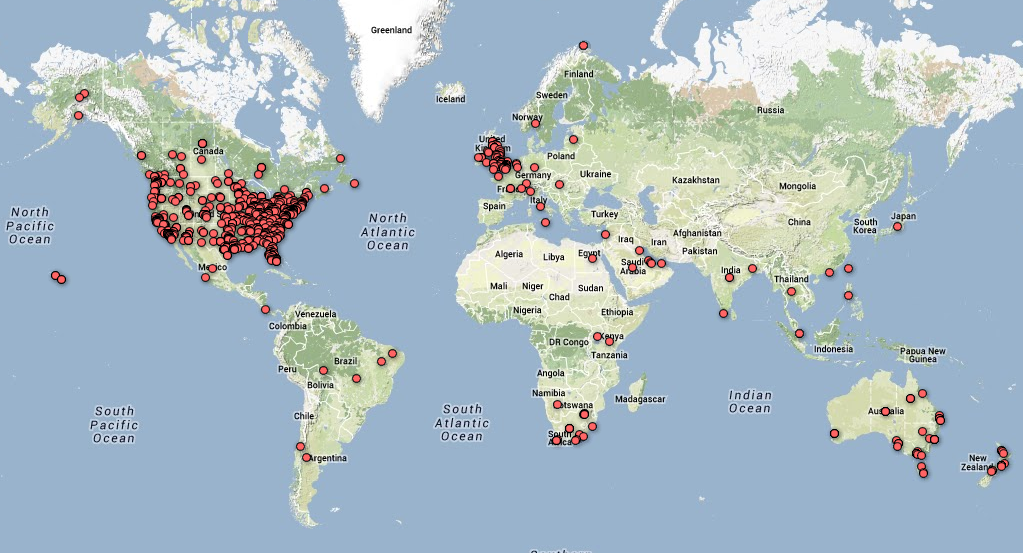
\includegraphics[width=0.61\linewidth]{../images/map3}
\caption{Stated locations of members}\label{fig:map}
\end{figure}

\begin{figure}[b]
\centering
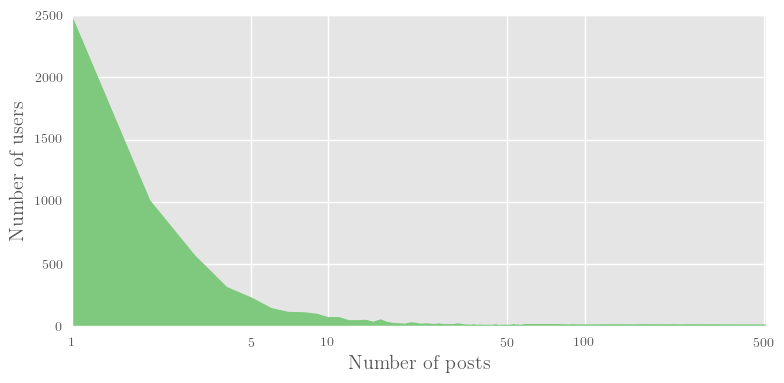
\includegraphics[width=0.70\linewidth]{../images/best-posts-users}
\caption{Total members by postcount}\label{fig:counts}
\end{figure}

Unlike in Maclean et al's analysis of \emph{Forum77} \parencite*{maclean_forum77:_2015}, \glslink{member}{users} who were active at the time of data collection were not excluded from the dataset. A potential effect of this is that the ratio of veteran to non\hyp{}veteran \glslink{member}{users} is slightly skewed toward non\hyp{}veteran \glslink{member}{users}, as some currently active members may eventually progress to become veteran members in the future.
%todo: removed because point already made?
%That said, the \glslink{forum}{Bipolar Forum} was in a state of rapid decline at the time of data collection. Therefore, very few \glspl{member} would have ultimately been removed according to the criteria of recent activity.

One final consideration regarding the \glslink{member}{user} base is that nothing prevents \glslink{member}{users} from creating and \glslink{post}{posting} from multiple accounts. As such, following \textcite{de_choudhury_discovering_2016}, the terms \emph{\glslink{member}{user}}, \emph{\gls{member}} and \emph{\glslink{member}{contributor}} refer more specifically to \glslink{member}{users'} accounts than to actual people who use the \glslink{Forum}{board}. That said, there is no evidence to suggest, and no reason to believe, that \glslink{member}{users} create and \gls{post} under multiple accounts.

\subsection{Justification for site selection}

The \gls{Forum} is a typical example of a large online \glslink{forum}{message board}. As discussed in Chapter \ref{chap:onlinehealth}, these kinds of communities are well\hyp{}studied, allowing more reliable connection of findings to earlier research into \glspl{OSG} than would be the case if the selected site was from an emerging \gls{mode} of \gls{CMC}. The fact that the \gls{Forum} has undergone few structural changes since 2001 is particularly useful, as it eliminates a potential confounding variable, where longitudinal changes in language use may be affected by changes in the ways \glslink{member}{users} create and transmit messages. While it is possible that hardware changes (faster web access, increased mobile usage, etc.) could have effects on language use, such effects also occur in other non\hyp{}researcher\hyp{}constructed communities. Compared to social networking sites and mobile apps, both of which typically undergo constant interface redesign, the \glslink{Forum}{Bipolar Forum} can be seen as relatively stable over time.

An important reason for selecting the \gls{Forum} is its size: with over eight million words of public \glspl{post}, it is large enough to make quantitative generalisations about language use not only in the \gls{corpus}, but also in its individual subcorpora. A large dataset increases the level of delicacy that can be quantitatively discussed, as delicate features are by definition rarer than broad features.

Another motivation for choosing the \gls{Forum} is its general Tenor, which is formal enough to be parseable with off\hyp{}the\hyp{}shelf parser models trained on formal English: correct capitalisation, punctuation and paragraph breaks are, for most \glslink{member}{users}, the norm. Texts authored for other varieties of \gls{CMC}, such as Twitter, may be much more difficult to parse, due to novel linguistic features such as hashtags, emoticons and embedded links.

%or chat services that may feature a great deal more non\hyp{}standard language, emoticons, emojis and the like.

The fact that the \gls{Forum} is text\hyp{}heavy and light on multimodal features is also useful, as this means that the \gls{CL} approach is quantifying a very large amount of the meaning\hyp{}making that occurs within the \glslink{Forum}{community}. In systemic terms, the \emph{division of labour} in the \glslink{member}{community} is almost entirely semiotic, rather than material; as such, text analysis takes us further in describing and explaining the \glslink{Forum}{community} than it would in a domain where much of the meaning\hyp{}making is material. This is the case even when comparing to other forms of \gls{CMC} (\emph{YouTube}, \emph{Instagram}, \emph{Snapchat}, etc.), where text comments play a secondary role to images, audio and\slash or video. Even so, because discourse analysis ideally involves analysis of texts in something resembling their original contexts, the \gls{HTML} content of all pages was retained, so that selected examples could be considered with sensitivity to extralinguistic meanings made by multimodal site features.

% Finally, the group is completely public: \glspl{post} are indexed within the site's own search tool, and by general search engines. Login is not required to view or search \glspl{post}. \glslink{member}{Users} are explicitly told that contributions are public in the FAQs and Terms and Conditions. From the main page, threads are annotated with the thread's total number of views, reminding users that \glspl{post} are seen by far more people than the interlocutors themselves. Finally, searching the \gls{corpus} for addresses, email addresses and phone numbers did not turn up a single instance that needed anonymisation. These factors all limit potential privacy concerns surrounding the harvesting of linguistic content from the site.

\section{Ethics}

%!TEX root = ../thesis.tex

% 12 june draft complete

The ethical parameters of the investigation were informed by consideration of:

\begin{enumerate}
    \item International research ethics literature that deals with \gls{CMC} and \glspl{OSG}
    \item The medium and situation factors unique to the \glslink{Forum}{Bipolar Forum}
    \item The \emph{Australian National Statement on Ethical Conduct in Human Research 2007 (updated May 2015)} \nocite{national_health_and_medical_research_council_the_australian_research_council_and_the_australian_vice-chancellors_committee_national_2015}
\end{enumerate}
%
The guidelines in the National Statement take precedence over the broader international literature. That said, the National Statement provides little guidance on \gls{CMC}, which often challenges existing notions of privacy, anonymity and informed consent. As such, consideration of ethical concerns raised in the relevant literature is prudent. Strategies employed to minimise risk to participants are also described.

\subsection{Considering \glsfmtshort{CMC}\slash \glsfmtshort{OSG} data}

Much has been written about the ethics of researching \gls{CMC} \cite{boyd_social_2007-1,ess_internet_2007,eysenbach_towards_2000,hewson_ethics_2015,landert_private_2011,stevens_public_2015,walther_research_2002}. Common is a recognition that different \glspl{mode} require different ethical considerations: forms of \gls{CMC} that can be easily connected to real\hyp{}world identities (due to the use of real names, profile photos, etc.) necessitate different protocols from forms that are highly anonymised. Similarly, the level of privacy and anonymity is not necessarily the same for all \glspl{mode}: on YouTube, video bloggers show their faces and often give their real names, while commenters on the clips are generally highly anonymised.

Another factor influencing ethical decisions is the size of the dataset. In the case of very large quantities of user\hyp{}generated natural language, it may become impossible for researchers to check that data has been fully anonymised. For these reasons, literature concerned with the ethics of using Facebook\slash chat data \cite[e.g.][]{hudson_``go_2004,zimmer_but_2010} or small\hyp{}scale, qualitative datasets \cite[e.g.][]{eysenbach_ethical_2001,roberts_ethical_2015} are not particularly relevant here.

The use of online \glspl{forum} as data sources has been a contentious issue. Though most acknowledge that \glspl{forum} are `public', the fact that \glslink{post}{contributions} are often authored in private spaces such as bedrooms may influence the candidness of texts \cite{hewson_ethics_2015}. Others have questioned the usefulness of the `public\slash private' binary in online contexts more generally \cite{lange_publicly_2007}. When compared to face\hyp{}to\hyp{}face data, researchers also know less in general about the participants, making it difficult to assess potential harm on an individual basis. In quantitative studies of thousands of users, spanning over a decade of \glslink{post}{contributions}, this becomes an impossibility.

Another issue is the potential for quotations, even when stripped of contextual information, to be linked back to their source: since texts in online \glspl{forum} are indexed in search engines, simply entering quotes into a search engine will often quickly uncover the original \gls{thread}. There, one can access the user's profile, and in some cases even send the user a private message. One strategy for avoiding this issue has been to paraphrase or translate quotes \cite{stommel_use_2011,vayreda_social_2009}. In an investigation of subtle changes in linguistic choices, however, this sacrifices the authenticity of the data.

%Related is the issue of what constitutes anonymity for online forum users. At what point do we say that a participant has been de-anonymised? The public profile of the user? The user's email address? The user's username? As with the issue of public vs. private information, contemporary debate frames anonymity as a continuum \cite{nagel_anonymity_2015}, rather than a binary.

%The level of privacy and anonymity is not necessarily the same for all interactants: on YouTube, video bloggers show their faces and often give their real names, while commenters on the clips are generally highly anonymised.

\textcite{hewson_ethics_2015} and \textcite{markham_ethical_2012} argue that flexible, bottom\hyp{}up, contextually sensitive parameters should be created for any study of \gls{CMC}. Accordingly, below, I summarise issues of privacy, anonymity and informed consent with respect to the specific medium and situation factors of the forum.

\subsubsection{Contact with participants} 

Participants were not contacted at any stage before, during or after the study. Therefore, none of the data was researcher\hyp{}elicited, and no non\hyp{}publicly available data were generated for the project. The National Statement includes `damage to social networks' (p.~13) as a kind of harm that research can do to participants. Not contacting \gls{Forum} \glslink{member}{users} therefore minimises harm by preserving an existing social structure as\hyp{}is. At the same time, the decision not to contact participants made it impossible to obtain informed consent. The highly anonymised nature of the board, as well as the longitudinal focus of the case study, however makes obtaining such consent from all \glslink{member}{contributors}, or even a plurality thereof, impossible \cite{kaufman2016producing,stommel_use_2011}. %In the case of this study, however, the issue is moot: as explained below, the National Statement exempts the study from the process of obtaining participants' consent.

\subsubsection{Anonymity and privacy}

Online spaces vary in the extent to which users' contributions are publicly accessible, and in how much users can reveal about their identity. In the \glslink{Forum}{Bipolar Forum}, \glslink{member}{users} protect their anonymity: they use nicknames, and do not contribute information that could identify them offline, such as real names, addresses, social security numbers, or photographs. In both the account creation and posting guidelines, \glslink{member}{users} are reminded to keep \gls{Forum} contents anonymous, and to assist in the anonymisation of others:

\begin{quote}
\small \singlespacing 
Do not register your surname or put identifying info in your profile or signature: Your username, profile, signature and messages must not identify you to readers or contain any part of your email address, blog or website. % http://www.healthboards.com/boards/faq.php?faq=faq_hb#faq_new_faq_item

Please only use first names of members. To protect anonymous use of the site do not include surnames. Use the listed first name or the username. % http://www.healthboards.com/boards/faq.php?faq=faq_hb#faq_poliguid

\end{quote}
%
Moderators also have the power to censor content that may de\hyp{}anonymise the user. Ultimately, \glslink{member}{users} appear to adhere to these rules: searching the \gls{corpus} for addresses, email addresses and phone numbers did not turn up a single instance that needed anonymisation, nor did any such information emerge throughout the course of the investigation.

%Again, the National Satement argues that exposing Participants' crimes can constitute harm `including discovery and prosecution of criminal conduct.' (p.~13)

Finally, all analysed data is publicly available. Though some researchers have problematised academic use of user\hyp{}generated \gls{CMC} \cite[e.g.][]{eysenbach_towards_2000,zimmer_but_2010}, such critiques centre on the notion that participants are unaware of the publicly available nature of their contributions. This is not a reasonable argument in the case of the \glslink{Forum}{Bipolar Forum},\endnote{Users' expectation of privacy is more likely to be an ethical issue in modes such as online chat, where chat messages appear to vanish after new messages arrive, and where chat transcripts are not searchable online, or connected through hyperlinks to a user's profile.} for a number of reasons:

\begin{enumerate}
    \item Users can see how many others are currently online, and how many people have viewed each thread.
    \item The main page invites users to \texttt{Subscribe} for an automatic bulletin of popular posts.
    \item Every page contains a \texttt{Search} button, showing that all posts are archived and indexed.
    \item Users' profiles are explicitly called \texttt{Public Profile Pages}. Help pages for Public Profile creation remind users that what they add is `publicly available'. %http://www.healthboards.com/boards/faq.php?faq=vb3_user_profile#faq_vb3_public_profile
\end{enumerate}
%
To argue that \gls{Forum} \glslink{member}{users} are not aware of the public nature of their interactions is to argue that \glslink{member}{users} fundamentally misunderstand the design and function of the community. No evidence supporting the idea that \glslink{member}{users} have such a misunderstanding was found over the course of the investigation.

% The linguistic content of their contributions consistently demonstrates that users are aware that their posts are read by strangers

\subsection{Interpreting the National Statement}

Under the National Statement, application for review and clearance from a Human Research Ethics Committee is required when the research carries more than a low risk of harm, distress or, at minimum, discomfort, to participants.\endnote{Under the National Statement, forum users qualify as participants, despite their not being contacted, or even being aware of the fact that their data is being analysed.} Exempted from the review process, however, is research that:

\begin{quote}
\small \singlespacing
\begin{enumerate}
    \item is negligible risk research; and
    \item involves the use of existing collections of data or records that contain only non\hyp{}identifiable data about human beings (p.~70).
\end{enumerate}
\end{quote}
%
The case study qualifies as negligible risk, as any potential risks for \gls{Forum} \glslink{member}{contributors} do not rise to the level of discomfort. The data qualifies as non\hyp{}identifiable, as they `have never been labelled with individual identifiers' (p.~27). More specifically, the \gls{Forum} data constitutes a subset of the non\hyp{}identifiable data class, which 

\begin{quote}
\small \singlespacing
are those that can be linked with other data so it can be known that they are about the same data subject, although the person's identity remains unknown (p.~27).
\end{quote}
%
It is indeed possible to connect different contributions to a single author due to the username (and potentially, the linguistic content of the contribution). This, however, cannot be connected to individual identifiers.

Because the case study is exempted from the process of ethics review, and due to the consideration of broader literature and site\hyp{}specific factors, an application for review was not made.

\subsubsection{Participants with mental health issues}

The majority of users of the \gls{Forum} may be classified as having a mental illness. The National Statement mandates that the `distinctive vulnerabilities' of such people must be taken into account, while also protecting the entitlement of such people to participate in research. Researching those with mental health issues may also involve differing guidelines for obtaining consent. According to the Statement, however, in cases where `research uses collections of non\hyp{}identifiable data and involves negligible risk', the need for informed consent is waived.

%It is also notable that the overall topic of the forum is less sensitive than topics that deviate from mainstream medical advice (such as pro-anorexia forums) and\slash or are potentially illegal, such as drug use or pedophilia forums, both of which have been studied using similar methods.

\subsection{Minimising risk}

Under the National Statement, `researchers have an obligation to minimise the risks to participants' (p.~14). To minimise any potential risk of privacy invasion, \glslink{member}{users'} public profiles were excluded from data collection, and usernames have been paraphrased throughout the thesis. Any part of the \gls{Forum} restricted to registered \glspl{member} was not accessed or considered in the analysis. The \gls{corpus} therefore includes only text that is freely accessible by navigating the \glslink{Forum}{Bipolar Forum}.

To ensure that no social structure is disturbed, and to ensure \glslink{member}{contributors'} privacy, all texts chosen for sustained, qualitative analysis are authored by \glslink{member}{users} who are now inactive within the \glslink{Forum}{community}, having not \glslink{post}{posted} in the past year.

\section{Corpus building}

In the following section, I describe the process of turning the \gls{Forum}'s contents into structured, annotated \glspl{corpus} (the \emph{Bipolar Forum Corpus}).

\subsection{Content retrieval}

All \glspl{thread} of the \glslink{forum}{Bipolar Forum} were downloaded as \gls{HTML} to a local machine using a purpose\hyp{}built tool, based on \texttt{GNU Wget}, on December 3rd, 2013. This 1.8GB collection of almost 19,000 files, including metadata (usernames, timestamps, users' locations, etc.) comprises the total dataset for the thesis.

\subsection{Corpus creation}

Python's \emph{lxml} module was used to extract the text and relevant metadata (e.g. speaker, timestamp, etc.) of \glspl{post} within each \gls{thread}. Regular expressions were used to search for details in text requiring anonymisation, such as addresses, email addresses and phone numbers. This did not turn up any personal details---the only matches were for emergency services, health\hyp{}related hotlines, and, more rarely, specific hospitals. For the sake of parser accuracy, some basic spelling normalisation was then performed. Apostrophes were reinserted: \emph{im} became \emph{i'm}, and \emph{whod} became \emph{who'd}. Ambiguous cases (\emph{shell, hell, wed, etc.}) were left uncorrected. Also changed were common contractions such as \emph{gonna} and \emph{wanna} into \emph{going to} and \emph{want to}. Alternative spellings of \emph{bipolar} (\emph{bi-polar, bi polar}) were also normalised. All other misspellings were left uncorrected. The results---the cleaned text of each post in the thread, and some its metadata features (\gls{post} count at time of \glslink{post}{posting}, date of \gls{post}, username, gender, location, etc.)---were then saved into text files representing each \gls{thread}. Below is an example of a single \gls{post} and its associated metadata in \gls{XML} form.

\begin{minted}[linenos,frame=single,xleftmargin=1cm,breaklines=true]{xml}
I hope everyone is hanging in with this blasted heat. As we all know being hot, sticky, stressed and irritated can bring on a mood swing super fast. So please make sure your all takeing your meds and try to stay out of the heat. <metadata username="Emz45" totalposts="5063" currentposts="4051" date="2011-07-13" postnum="0" threadlength="1"
\end{minted}
%
\noindent The tools developed for the investigation (see Section \ref{sect:corpkit}) were then used to extract the metadata, parse each cleaned text with the \emph{Stanford CoreNLP 3.6.0} pipeline, and to reintroduce the metadata to the parser output. The result of this process was a large collection of files in \emph{CONLL\hyp{}U} format \cite{nivre_towards_2015}---an example of the parsed representation of the \gls{post} above is presented in Figure \ref{fig:parsed-text}. In this representation, the columns are \emph{token index}, \emph{token}, \emph{lemma}, \gls{POS}, \emph{named\hyp{}entity tag}, \emph{governor}, \emph{dependency type}, \emph{dependent(s)}, and \emph{coreferences}. The two rightmost columns are not a part of the CONLL\hyp{}U specification, but have been added by \texttt{corpkit} during post\hyp{}processing to speed up interrogations at runtime. Note that the constituency parse is treated as a metadata feature, so as to not violate the format specifications.

\begin{figure}[htb]
\begin{minted}[linenos,frame=single,xleftmargin=1cm,breaklines=true]{text}
# sent_id 1
# parse=(ROOT (S (NP (PRP I)) (VP (VBP hope) (SBAR (S (NP (NN everyone)) (VP (VBZ is) (VP (VBG hanging) (PP (IN in) (IN with) (NP (DT this) (VBN blasted) (NN heat)))))))) (. .)))
# speaker=Emz45
# totalposts=5063
# threadlength=1
# currentposts=4051
# stage=10
# date=2011-07-13
# year=2011
# postnum=0
1   I         I         PRP O   2   nsubj      0       1
2   hope      hope      VBP O   0   ROOT       1,5,11  _
3   everyone  everyone  NN  O   5   nsubj      0       _
4   is        be        VBZ O   5   aux        0       _
5   hanging   hang      VBG O   2   ccomp      3,4,10  _
6   in        in        IN  O   10  case       0       _
7   with      with      IN  O   10  case       0       _
8   this      this      DT  O   10  det        0       2
9   blasted   blast     VBN O   10  amod       0       2
10  heat      heat      NN  O   5   nmod:with  6,7,8,9 2*
11  .         .         .   O   2   punct      0       _
\end{minted}
\caption[A parsed sentence with metadata]{A sentence from the Forum, parsed and stored alongside metadata in CONLL-U format}
\label{fig:parsed-text}
\end{figure}

The texts were put into ten subfolders, representing each of the ten stages of membership. This is the default subcorpus format recognised by the interrogation tool. To investigate a different structure, such as language use in the \gls{Forum} by year, the tool can simply be told to treat the \texttt{year} metadata values as the subcorpora. In this way, it is possible to use the same \gls{corpus} to answer address a number of possibl research questions. Setting \texttt{speaker} as subcorpora would create subcorpora for each of the 5,818 unique members (See Table \ref{tab:p_stats}), allowing, for example, ranking of \glslink{member}{users} according to some linguistic criterion. Setting \texttt{gender} as subcorpora would allow investigation of differences in the language use of those who identify as male, as female, and those who choose not to provide their gender. As the main concern of this thesis is linguistic change over the membership course, however, almost all querying of the corpus targeted the membership stage variable (the \texttt{stage} metadata). That said, other structures are also briefly utilised, in order to control for self\hyp{}selection bias. An overview of each of the four symbolic subcorpus structures is given in the sections below.

%It is important to note that the investigation focusses almost exclusively on the first of these \glspl{corpus} (\emph{P Corpus}, which groups every contribution to the \gls{Forum} into ten subcorpora based on how many previous \glspl{post} a user had made at the time of posting. The other three \glspl{corpus} are not core objects of study in the thesis; rather, they are simply designed to augment it (by mapping change in users' language to the \gls{Forum}'s history), and to address possible limitations caused by its structural composition. The auxiliary \glspl{corpus} contain no text that is not also available in the main \gls{corpus}: they are either subsets of it, or structural rearrangements of it.

\subsubsection*{\emph{Membership Stage Structure}}

The main subcorpus structure used in the thesis is the \emph{Membership Stage Structure}, which consists of ten subcorpora of almost equal size, approximating ten `stages of membership'. The first subcorpus contains all first \glspl{post} to the \gls{Forum}. The number of \glspl{post} in this sub\hyp{}folder (5,818) dictated the sample size for the next subcorpus. The second subcorpus contained each user's second and third \glspl{post}; the third subcorpus contained \glspl{post} 4--7, and so forth. This structure makes it possible to learn \emph{how language changes over the course of membership in the community}. Table \ref{tab:p_stats} provides an overview of the composition of each subcorpus. Table \ref{tab:shallow_P} provides absolute frequencies for shallow linguistic features. These features are among those used to generate shallow findings in Chapter \ref{chap:introdata}, and to aid in the calculation of relative frequencies in Chapters \ref{chap:interpersonal} and \ref{chap:experiential}.

It is important to note that this structure operationalises \emph{veteran membership} entirely according to a \glslink{member}{user's} number of \glspl{post}. This unidimensional approach has the advantage of simplicity, making it possible to examine the question of \emph{how \gls{post} count affects language use}. At the same time, using a single feature to segment the data means that segmentation is not based on algorithm whose efficacy has not yet been proven in other contexts. It is theoretically simplistic, however---as mentioned in Section \ref{sect:vetmemb}, ideally, veteran membership would be determined based on a number of factors including not just number of \glspl{post}, but duration of membership, the average number of replies received, and any explicit privileges the user may have within the community. \textcite{pfeil_social_2011}, for example, provide an alternative method of differentiating between \gls{forum} members, clustering users by similarity in contributing behaviour (who users reply to) and the effects of this behaviour (who responds to the contribution). In descriptions and analysis that follow, unless otherwise noted, \emph{Veteran membership} refers to Subcorpus 10, and \emph{New members} refer to Subcorpus 1. It should be borne in mind, however, that a veteran \gls{post} or contribution is nothing more than a contribution made by a \glslink{member}{user} who has already \glslink{post}{posted} at least 559 times before.

\begin{table}[htb]
\centering
\footnotesize
\begin{tabularx}{1\textwidth}{Xrrrrrrrrrr}

\toprule
Subcorpus & $01$ & $02$ & $03$ & $04$ & $05$ & $06$ & $07$ & $08$ & $09$ & $10$ \\ \midrule
Post range & $1    $      &  $ 2\mbox{--}3  $   & $4\mbox{--}7 $    & $8\mbox{--}15$    & $16\mbox{--}30$ & $31\mbox{--}58$   &  $59\mbox{--}115$  & $116\mbox{--}219$ & $220\mbox{--}559$  & $560+$  \\
Texts      & $5,818$      &  $ 5,689 $   & $5,607$    & $5,937 $    & $5,790 $ & $5,875 $   &  $5,848  $  & $5,757   $ & $5,789$    & $5,570$ \\
Users     &  $5,818$      &  $ 3,348 $   & $1,777$    & $1,004$    & $ 529  $ & $284   $   &  $148    $  & $76      $ & $38$       &   $8$ \\ \bottomrule
\end{tabularx}
\caption[Membership Stage Structure: subcorpus attributes]{Bipolar Forum Corpus, Membership Stage Structure: key attributes of each subcorpus}
\label{tab:p_stats}
\end{table}


\begin{table}[htb]
\centering
\small
\begin{tabular}{lrrrrrrr}
\toprule
{} &  Characters &   Tokens &    Words &  Closed class &  Open class &  Clauses &  Sentences \\
\midrule
$01$ &     $4,380,658$ & $1,258,606$   &  $1,092,113$ &        $643,779$ &      $614,827$ &   $277,103$ &      $68,267$ \\
$02$ &     $3,185,042$ &   $922,243$   &    $800,046$ &        $471,883$ &      $450,360$ &   $209,448$ &      $51,575$ \\
$03$ &     $3,157,277$ &   $917,822$   &    $795,517$ &        $471,578$ &      $446,244$ &   $209,990$ &      $51,860$ \\
$04$ &     $3,261,922$ &   $948,272$   &    $820,193$ &        $486,065$ &      $462,207$ &   $216,739$ &      $53,995$ \\
$05$ &     $3,164,919$ &   $921,098$   &    $796,430$ &        $473,446$ &      $447,652$ &   $210,165$ &      $52,227$ \\
$06$ &     $3,187,420$ &   $928,350$   &    $797,652$ &        $480,843$ &      $447,507$ &   $209,895$ &      $52,171$ \\
$07$ &     $3,080,956$ &   $900,110$   &    $771,319$ &        $466,254$ &      $433,856$ &   $202,868$ &      $50,071$ \\
$08$ &     $3,356,241$ &   $972,652$   &    $833,135$ &        $502,913$ &      $469,739$ &   $218,382$ &      $52,637$ \\
$09$ &     $2,908,221$ &   $840,803$   &    $725,108$ &        $434,839$ &      $405,964$ &   $191,851$ &      $47,050$ \\
$10$ &     $2,868,652$ &   $815,101$   &    $708,918$ &        $421,403$ &      $393,698$ &   $185,677$ &      $43,474$ \\
\bottomrule
\end{tabular}
\caption{Shallow features of the \emph{Membership Stage Structure}}
\label{tab:shallow_P}
\end{table}

\subsubsection*{\emph{Future Veteran Structure}}

The second structure, the \emph{Future Veteran Structure}, is a subset of the Membership Stage Structure, with any \glslink{post}{contribution} from \glslink{member}{users} with fewer than 30 total \glspl{post} removed. This structure makes it possible to \emph{isolate veteran members' language change}, accounting for a potential self\hyp{}selection bias, where those who go on to become veterans have different linguistic patterns even during their initial \glslink{post}{contributions}. The removal of non\hyp{}future\hyp{}veteran contributions means that there are very few \glspl{post} in the first four subcorpora. For this reason, during analysis, the first four subcorpora are conflated, in order to keep subcorpora quantitatively reliable in terms of word count.

\begin{table}[htb]
\centering
\small
\begin{tabular}{lrrrrrrr}
\toprule
{} &  Characters &  Tokens &   Words &  Closed class &  Open class &  Clauses &  Sentences \\
\midrule
$01\mbox{--}04$ &    $2,520,668$ &  $729,694$ &  $631,438$ &        $375,581$ &   $354,113$ &   $165,348$ &      $40,332$ \\
$05$    &            $2,360,495$ &  $687,311$ &  $593,178$ &        $354,671$ &   $332,640$ &   $156,941$ &      $38,776$ \\
$06$    &            $3,187,420$ &  $928,350$ &  $797,652$ &        $480,843$ &   $447,507$ &   $209,895$ &      $52,171$ \\
$07$    &            $3,080,956$ &  $900,110$ &  $771,319$ &        $466,254$ &   $433,856$ &   $202,868$ &      $50,071$ \\
$08$    &            $3,356,241$ &  $972,652$ &  $833,135$ &        $502,913$ &   $469,739$ &   $218,382$ &      $52,637$ \\
$09$    &            $2,908,221$ &  $840,803$ &  $725,108$ &        $434,839$ &   $405,964$ &   $191,851$ &      $47,050$ \\
$10$    &            $2,868,652$ &  $815,101$ &  $708,918$ &        $421,403$ &   $393,698$ &   $185,677$ &      $43,474$ \\
\bottomrule
\end{tabular}
\caption[Shallow features of the \emph{Future Veteran Structure}]{Shallow features of the \emph{Future Veteran Structure}, with subcorpora 1--4 collapsed}
\label{tab:shallow_V}
\end{table}

\subsubsection*{\emph{Longitudinal Structure}} \label{sect:l-corpus}

The third structure, the \emph{Longitudinal Structure} is chronological, with 13 annual subcorpora. In this structure, \glspl{thread}, rather than \glspl{post}, can become the unit of analysis. This structure makes it possible to observe phylogenesis---that is, \emph{longitudinal change in the norms of the \gls{Forum} itself} that result from the constant stream of incoming and outgoing members.

\begin{table}[htb]
\centering
\small
\begin{tabular}{lrrrrrrr}
\toprule
{} &  Characters &   Tokens &    Words &  Closed class &  Open class &  Clauses &  Sentences \\
\midrule
$2001$ &    $   21,743$ &  $   6,061  $ &  $    5,197   $ &    $    2,938$  &   $     3,123$ &   $  1,272$ &  $   333 $  \\
$2002$ &    $  193,771$ &  $  55,979  $ &  $   47,920   $ &    $   28,291$  &   $    27,688$ &   $ 12,752$ &  $  2,807$  \\
$2003$ &    $ 2,283,828$ & $ 656,838  $ &  $  568,429   $ &    $  332,839$  &   $   323,999$ &   $146,266$ &  $ 29,394$  \\
$2004$ &    $ 2,484,517$ & $ 708,587  $ &  $  613,078   $ &    $  358,589$  &   $   349,998$ &   $149,217$ &  $ 30,810$  \\
$2005$ &    $ 4,710,146$ & $1,366,425 $ &  $  1,176,398  $ &    $   699,091$  &   $   667,334$ &   $304,403$ &  $ 60,756$  \\
$2006$ &    $ 6,512,854$ & $1,851,707 $ &  $  1,627,163  $ &    $   945,150$  &   $   906,557$ &   $429,597$ &  $ 85,598$  \\
$2007$ &    $ 8,827,854$ & $2,525,622 $ &  $  2,221,659  $ &    $  1,292,264$  &   $   233,358$ &   $590,495$ &  $114,341$  \\
$2008$ &    $ 2,634,440$ & $ 762,596  $ &  $  662,350   $ &    $  388,076$  &   $   374,520$ &   $172,333$ &  $ 37,527$  \\
$2009$ &    $ 4,653,461$ & $1,328,212 $ &  $  1,159,234  $ &    $   674,634$  &   $   653,578$ &   $303,264$ &  $ 61,381$  \\
$2010$ &    $  931,807$ &  $ 264,611  $ &  $  232,084   $ &    $  133,755$  &   $   130,856$ &   $ 58,713$ &  $ 12,806$  \\
$2011$ &    $  890,052$ &  $ 253,953  $ &  $  222,752   $ &    $  128,321$  &   $   125,632$ &   $ 55,440$ &  $ 11,442$  \\
$2012$ &    $  392,618$ &  $ 111,959  $ &  $   97,118   $ &    $   56,020$  &   $    55,939$ &   $ 24,149$ &  $  5,597$  \\
$2013$ &    $  202,393$ &  $  56,803  $ &  $   49,623   $ &    $   28,634$  &   $    28,169$ &   $ 12,711$ &  $  2,859$  \\
\bottomrule
\end{tabular}
\caption{Shallow features in the \emph{Longitudinal Structure}}
\label{tab:shallow_L}
\end{table}

\begin{figure}[htb]
\centering
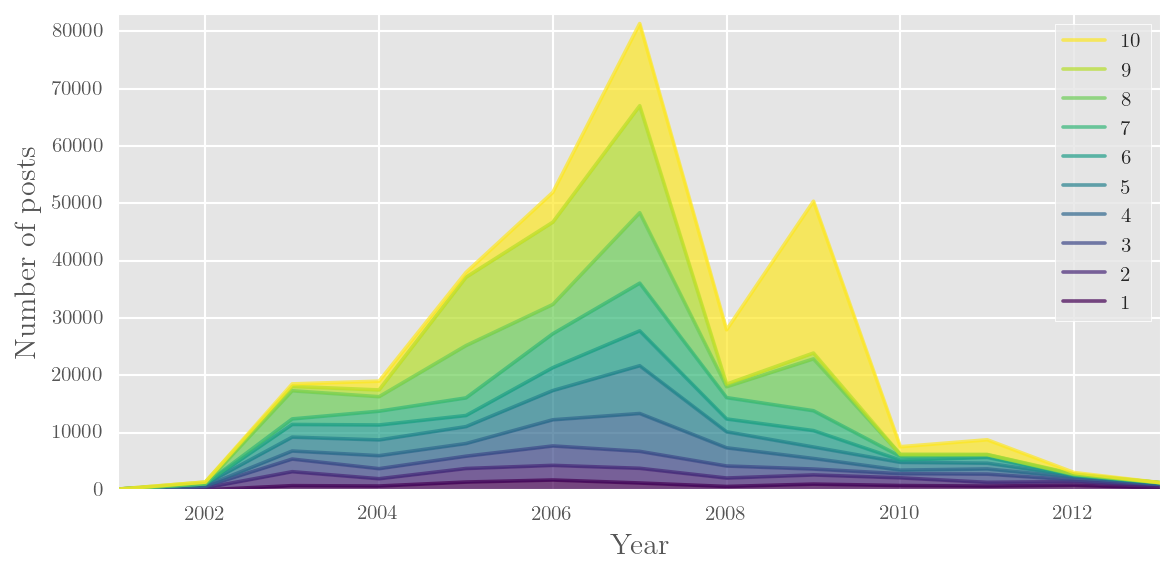
\includegraphics[width=0.75\textwidth]{../images/posts-by-year.png}
\caption[Number of posts in the \emph{Longitudinal Structure}]{Number of posts in the \emph{Longitudinal Structure} by membership stage}
\label{fig:stage_year}
\end{figure}

\begin{figure}[htb]
\centering
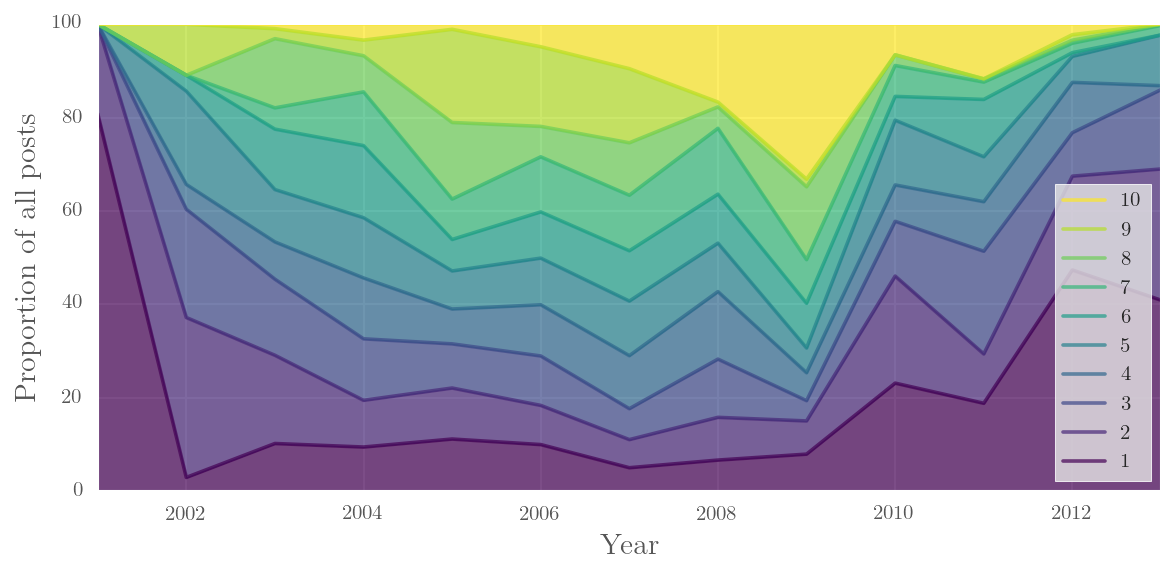
\includegraphics[width=0.75\textwidth]{../images/posts-by-year-filled.png}
\caption[Relative number of posts in the \emph{Longitudinal Structure}]{Relative number of posts in the \emph{Longitudinal Structure} by membership stage}
\label{fig:stage_year_filled}
\end{figure}

\begin{figure}[htb]
\centering
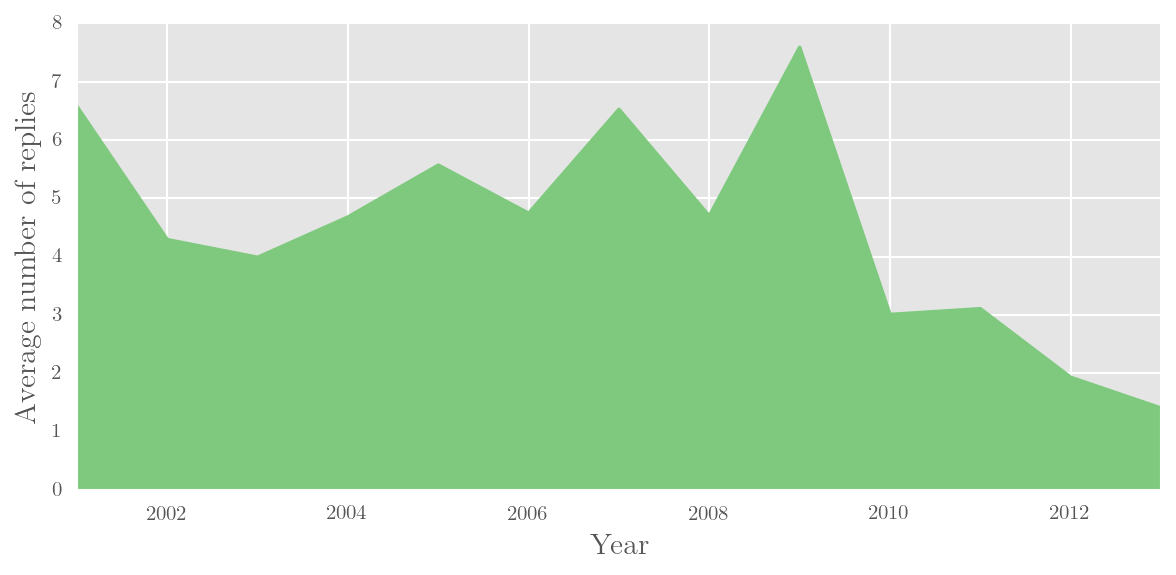
\includegraphics[width=0.75\textwidth]{../images/avg-replies.png}
\caption[Replies to new threads in the \emph{Longitudinal Structure}]{Average number of replies to new threads in the \emph{Longitudinal Structure}}
\label{fig:avg_replies}
\end{figure}

Figure \ref{fig:stage_year} uses the Longitudinal Structure to provide an overview of the amount of activity within the \gls{Forum} by year. The number of \glspl{post} steadily increases until 2009, at which point there is a similarly steady decline. Figure \ref{fig:stage_year_filled} shows the extent to which different membership stages are represented in the \gls{Forum} in a given year. Having information about the composition of membership stages at different points in time makes it possible to speculate as to what a low or high concentration of veteran members does to language use in the \glslink{Forum}{community} as a whole. This is not, however, a focus of the thesis.

Figure \ref{fig:stage_year_filled} shows that in the busiest years of the \gls{Forum}'s history, veteran \glspl{member} made proportionally more \glspl{post}.\endnote{It is important to remember that since a user must \gls{post} 560 or more times to enter the last stage of membership, veteran \glslink{member}{users} in the earlier years of the \gls{Forum}'s existence are bound to be less common.}~These members then gradually stop \glslink{post}{posting}; in the latest years sampled, many newcomers \gls{post} a question, but receive no reply (see Figure \ref{fig:avg_replies}). Combined, the smaller number of overall \glspl{post}, the departure of veteran \glspl{member}, and lack of follow\hyp{}up to new \glspl{thread} are taken as indicators that the \gls{Forum} is moribund.

\subsubsection*{\emph{Comparative Structure}}

The final structure, the \emph{Comparative Structure} consists of two subcorpora. In the first are the first 30 \glspl{post} of \glslink{member}{users} who did not progress beyond 30 \glspl{post} (`Dropouts'). In the second are the first 30 \glspl{post} of those \glslink{member}{users} who did (`Future veterans'). This structure makes it possible to \emph{check for differences in the early\hyp{}stage language of future\hyp{}veterans and early dropouts}. It is designed to address the possibility that there is a pre\hyp{}existing difference in the linguistic features of \glspl{member} who drop out early and \glspl{member} who become veterans.

\begin{table}[htb]
\centering
\footnotesize
\begin{tabular}{lrrrrrrr}

\toprule
{} &  Characters &   Tokens &    Words &  Closed class &  Open class &  Clauses &  Sentences \\
\midrule
Dropout        &    $15,480,624$ &  $4,478,616$ &  $3,883,247$ &  $2,293,005$ &           $2,185,611$ &  $1,011,519$ &     $252,142$ \\
Fut. vet. &    $17,070,684$ &  $4,946,441$ &  $4,257,184$ &  $2,559,998$ &           $2,386,443$ &  $1,120,599$ &     $271,185$ \\
\bottomrule
\end{tabular}
\caption{Shallow features in the \emph{Comparative Structure}}
\label{tab:shallow_C}
\end{table}


\section{\texttt{corpkit}: tools for corpus building and analysis} \label{sect:corpkit}

Data analysis involved the use of a purpose\hyp{}built \texttt{Python}\hyp{}based toolkit, \texttt{corpkit}. In this section, I explain the need for the tool, its development, core functionality, and significance within the research area. Complete documentation of its programmatic, graphical and interpreter interfaces is available via \texttt{\href{https://www.github.com/interrogator/corpkit}{https://www.github.com/interrogator/corpkit}}.

\subsection{Rationale for tool development}

Before analysing the \gls{corpus} data, a survey of existing tools for corpus analysis was conducted, with a number of criteria in mind:

\begin{enumerate}
\item Feature-richness: ability to perform lemmatisation, lexical and grammatical searches, handling of plain text, \gls{POS} tags, constituency and dependency parses
\item Automatability: ability to loop through subcorpora, or through lists of queries, or cycling through options such as lemmatisation, removal of closed\hyp{}class words, etc.
\item Flexibility: ability to add to wordlists, edit interrogation results (merging search results, spanning subcorpora, etc.)
\item Sensitivity to functional grammar(s): ability to operationalise functional linguistic notions when interrogating corpora and editing results (i.e. locate Events within Processes)
\item Visualisation: ability to generate useful visualisations of language use without the need to export data from the tool
\end{enumerate}
%
In addition to these selection criteria, preference was given to resources that were:
%
\begin{enumerate}
\item Open-source, freely available, non\hyp{}proprietary
\item Command\hyp{}line based, rather than graphical (to facilitate automation, replicability, etc.)
\end{enumerate}
%
With these criteria in mind, the following tools were tested for suitability:
%
\begin{multicols}{3}
\begin{enumerate}
\item \texttt{NLTK}
\item \texttt{WMatrix}
\item \texttt{AntConc}
\item \texttt{CasualConc}
\item \texttt{Wordsmith Tools}
\item \texttt{Sketch Engine}
\item \texttt{UAM Corpus Tool}
\item \texttt{Tregex}
\item \texttt{\gls{CWB}\slash CQP}
\end{enumerate}
\end{multicols}
%
\noindent Though individual features from each tool were useful, none satisfied all selection criteria. Shifting between tools during different stages of the investigation was also unfeasible, as much interrogation was exploratory, iterative, or cyclical. \texttt{UAM Corpus Tool}, while able to handle multiple subcorpora, and while providing systemic\hyp{}functional conversions of \texttt{Stanford CoreNLP} parses, was also not suitable, as it:
%
\begin{enumerate}
\item Struggled to cope with the size of the corpus\endnote{\texttt{UAM Corpus Tool}'s creator, Mick O'Donnell, has since re\hyp{}factored the tool to handle very large datasets.}
\item Had stability issues (for example, when exporting interrogation results)
\item Is \gls{GUI}\hyp{}based, and cannot be scripted
\item Does not grant the user direct access to the systemic\hyp{}functional parses or the parser itself, making it difficult to verify the accuracy of converted parses\endnote{O'Donnell is preparing to release much of the non\hyp{}\gls{GUI} code as open\hyp{}source (personal communication, 2015).}
\item Requires exporting data in order to sort or visualise results
\end{enumerate}
%
Command\hyp{}line tools such as the \texttt{Open Corpus Workbench} \cite{evert2011twenty} provided the necessary ability to perform iterative and recursive searches, but lacked the ability to extract complex features from full syntactic parser output, and to easily interface with state\hyp{}of\hyp{}the\hyp{}art tools for manipulating and visualising data. \texttt{Tregex} \cite{levy2006tregex}, a search query language for constituency trees, is able to perform complex queries, but does not handle lemmatisation, keyword calculation or advanced result manipulation. \texttt{NLTK} \cite{bird2009natural}, while containing routines for many linguistic tasks, did not provide an interface to parsing or interrogating \texttt{CoreNLP} dependency parser output,\endnote{More recent releases of \texttt{NLTK} have better integration with \texttt{Stanford CoreNLP}.} and did not provide a holistic interface for more general workflows. Given these considerations, the development of purpose\hyp{}built tools was the best solution, providing increased transparency and reproducibility of this investigation, while also being useful for other researchers interested in functional \gls{CL}.

\subsection{Contents of the toolkit}

\texttt{corpkit} is a \texttt{Python} module designed to create and interrogate parsed and structured \glspl{corpus}, edit interrogation results, and to display\slash visualise edited output. It is available as open\hyp{}source software:

\begin{enumerate}
    \item GitHub: \texttt{\href{https://www.github.com/interrogator/corpkit}{https://www.github.com/interrogator/corpkit}}
    \item PyPI: \texttt{\href{https://pypi.python.org/pypi/corpkit}{https://pypi.python.org/pypi/corpkit}}
    \item Documentation: \texttt{\href{http://corpkit.readthedocs.org/}{http://corpkit.readthedocs.org/}}
    \item Standalone app: \texttt{\href{http://interrogator.github.io/corpkit/}{http://interrogator.github.io/corpkit/}}
\end{enumerate} 
%

The toolkit is \emph{object\hyp{}oriented}. Users instantiate \glspl{corpus} as objects, which have methods for parsing, interrogating and concordancing. Interrogations are also objects, which have methods for editing, the calculation of statistics, saving and visualising. A basic workflow using the Python \gls{API} involves the following steps:

%\todo{Workflow as algorithm}

\begin{enumerate}
    \item Create a project to house corpus\slash \glspl{corpus}, saved data, images, wordlists \\ (\texttt{new\_project()} function)
    \item Instantiate plaintext corpus \\ (\texttt{Corpus} class)
    \item Parse plaintext corpus using \texttt{Stanford CoreNLP} \\ (\texttt{Corpus.parse() method})
    \item Interrogate\slash concordance parsed corpus for \glslink{lexicogrammar}{lexicogrammatical} phenomenon \\ (\texttt{Corpus.interrogate()} method)
    \begin{itemize}
        \item Constituency parses via \texttt{Tregex}\slash \texttt{nltk\_tgrep}
        \item Dependency parses via \texttt{pandas}
    \end{itemize}
    \item Edit results \\ (\texttt{Interrogation.edit()} method)
    \begin{itemize}
        \item Keeping, removing, merging entries or subcorpora
        \item Calculating relative frequencies
        \item Sorting, generating statistics, doing linear regression
        \item Keywording
    \end{itemize}
    \item Tabulate, export or visualise edited results \\ (\texttt{Interrogation.visualise()} method)
    \item Save data to project \\ (\texttt{Interrogation.save()} method)
\end{enumerate}
%
\texttt{Interrogation} objects store a dictionary of the parameters that created them, so that they can easily be reproduced. Saved interrogation results are loaded as \gls{corpus} attributes at the beginning of each session, simplifying the process of managing projects involving multiple \glspl{corpus}.

\subsubsection{Key design parameters}

The tool was designed in response to the needs of the case study, to noted shortcomings of existing tools, and to a small body of literature describing needs in the future generation of \gls{corpus} tools \cite[e.g.][]{anthony_critical_2013,anthony_developing_2006,gries_50-something_2013}. \textcite{anthony_critical_2013} provide a succinct summary of needed tool development:

\begin{quote} \small \singlespacing
[Linguistic research] will rely increasingly on large corpora, advanced functionality, and sophisticated statistical methods. \ldots~\Gls{corpus} tool development should be an open source initiative with tool components being developed in a modular fashion. By dividing tool components in this way, it becomes easier for tool functions and features to be extended, modified, or simplified depending on the need' \parencite*[pp.~155--156]{anthony_critical_2013}.
\end{quote}
%
\texttt{corpkit} responds to each of these parameters: it is built to work with \glspl{corpus} of any size, and to allow multiprocessing to speed up queries over very large datasets; it has the most advanced functionality of any corpus interrogation tool to date, with support for parsing, interrogating parser output, and distinguishing between subcorpora and metadata tags or values; it integrates with \texttt{scipy} \cite{scipy2001} and \texttt{pandas} \cite{mckinney_pandas_2010} in order to allow complex mathematical operations; it is free and open\hyp{}source; it is modular, interfacing with dedicated modules for editing, storing and visualising; graphical and command\hyp{}line interfaces tailored to programming and non\hyp{}programming linguists.

\subsection{Interfaces and functionality of the tool}

\texttt{corpkit} includes three different interfaces. The \gls{API} itself, used for all data analysis in the thesis, is the most powerful, but requires knowledge of Python. The other two interfaces---a graphical application, and a natural language interpreter---call the \gls{API} as a backend. These interfaces were developed with the aim of increasing the potential users of the tool to those without a background in computer programming. At the same time, because users can shift freely between interfaces, it was hoped that the tool could facilitate increasingly programmatic workflows in \gls{CL}. In the sections below, I explain the functionality of the tool, giving examples from the \gls{API}. The graphical and interpreter interfaces are introduced later.

\subsubsection{API}

The most complex interface is the \gls{API}, implemented in Python. Through this interface, users can access the full range of methods for a given object, and take advantage of common programming constructs, such as the writing of loops or conditional statements. It is the interface used for the case study itself. The \gls{API} is also the interface with the most potential use for computationally intensive downstream applications in the area of medical\slash clinical \gls{NLP}: it could easily be scripted to automatically parse, categorise and search new data as it becomes available.

\paragraph{\texttt{Corpus}}

The \texttt{Corpus} class models a directory (and optionally, subdirectories) of data files, which may be plain text files or \texttt{CONLL-U} data. Though the toolkit is oriented toward parsed and structured data, basic functionality for interrogating and concordancing is available for plain text \glspl{corpus} as well. \texttt{Corpus} objects have a \texttt{parse} method, which is essentially a wrapper around \texttt{Stanford CoreNLP}, with keyword arguments for annotators, memory allocation and so on. In the example below, a plaintext \texttt{Corpus} object is created and parsed with \texttt{Stanford CoreNLP} using default parameters.

\begin{minted}[linenos,frame=single,xleftmargin=1cm]{python}
from corpkit import Corpus
unparsed = Corpus('forum')
corpus = unparsed.parse()
\end{minted} 
%
This method returns another \texttt{Corpus} object representing the parsed data, which can then be interrogated and concordanced in complex ways. Each subcorpus and file is represented as \texttt{Subcorpus} and \texttt{File} objects respectively, which can also be interrogated and concordanced:

\begin{minted}[linenos,frame=single,xleftmargin=1cm]{python}
parsed['01']
# <corpkit.corpus.Subcorpus instance: 01>
parsed['01'].files[245]
# <corpkit.corpus.File instance: thread-4450244.txt.conll>
\end{minted}

\paragraph{Speaker segmentation}

One innovation in \texttt{corpkit}'s \texttt{parse} method is the addition of speaker segmentation. The \texttt{parse} method has a \texttt{speaker\_segmentation} argument, which will add speaker names to \texttt{CoreNLP} output, provided they are delineated with a colon at the start of a line, or by \gls{HTML}\slash \gls{XML} tags in the text. The process of speaker segmentation involves:

\begin{enumerate}
\item Creating a duplicate corpus with names removed
\item Parsing the duplicated corpus
\item Using character offset metadata in the parser output to find the original line in the duplicated text
\item Lifting the speaker name from the original corpus
\item Adding the speaker name to the parser output
\end{enumerate}
%
% todo: revise for truth
The Bipolar Forum Corpus also has speaker names included in the annotations, so that interrogations can be restricted to a particular \glslink{member}{user} or set of \glslink{member}{users}. It is therefore also possible to look for differences between how newcomer and veteran \glslink{member}{users} use language in one or more \glspl{thread}. At a broader level, this method makes it possible to computationally model register features of dialogic text, facilitating context\hyp{}responsive parsing (see Chapter \ref{chap:implications}). Such tasks are beyond the scope of the current investigation, however.

\paragraph{\texttt{Corpus.interrogate() method}}

As explained in the previous chapter, \gls{CL} is centrally concerned with extracting frequency information from texts. Generally speaking, researchers are interested in either counting the occurrences of a particular linguistic feature in each subcorpus (e.g. counting a particular word or grammatical feature), or in counting the possible realisations of a linguistic feature (counting the frequencies of every word that is a noun, or every subject in a passive construction). Perhaps surprisingly, few tools provide an interface for doing this kind of searching or counting. \texttt{corpkit} focusses on iterating over subcorpora, extracting complex \glslink{lexicogrammar}{lexicogrammatical} features, and tabulating the results.

The \texttt{Corpus.interrogate()} method, more precisely, centres on a three\hyp{}step process of \emph{searching}, \emph{excluding} and \emph{showing} (Figure \ref{fig:mod-of-doc}). Searching and excluding involve the specification of one or more combinations of \emph{search objects} and regular expression or wordlist\hyp{}based patterns to match. Search objects are broken down into a token of interest (i.e. a token, its governor, one of its collocates, etc.) and its attributes (i.e. its word form, its lemma form, its \gls{POS}, etc.---see Table \ref{tab:search-exclude-show}). The \texttt{GL} search object, for example, searches for any lemma form matching a pattern, returning the ID of its dependent(s). After each search criterion has been processed, indices of tokens are removed if they appear fewer times than the total number of search criteria---that is, tokens must match all search criteria by default. Then, any explicit excluding is performed, using the same syntax as searching: if a token matches the exclusion criteria, it is filtered from the set of matches. After exclusion is complete, a function is called that determines how to represent the search matches. If the user inputs \mintinline{python}{show=[I, P, L, GL]}, the program will output the index, \gls{POS}, lemma form and governor's lemma form of a match (e.g. \mintinline{python}{'2/NNS/user/be'}). Results are returned as a two\hyp{}dimensional array of counts for each shown object in each subcorpus. Figure \ref{fig:mod-of-doc} provide an examples of this method for constituency and dependency parses. In both cases, lemmatised adjectives modifying terms for doctors are returned. This produces the results shown in Table \ref{conc:adj_mod_doc_example}.

\begin{table}[htb]
\centering
\small
\begin{tabular}{lrrrrrrrr}
\toprule
{} & Match & Gov. & Dep. & Coref Head & N-gram & Collocate & 1L & 1R \\
\midrule
Word          &     \texttt{W} &       \texttt{GW} &        \texttt{DW} &        \texttt{HW} &     \texttt{NW} &        \texttt{BW} &        \texttt{-1W} &        \texttt{-1W} \\
Lemma          &     \texttt{L} &       \texttt{GL} &        \texttt{DL} &        \texttt{HL} &     \texttt{NL} &        \texttt{BL} &        \texttt{-1L} &        \texttt{-1L} \\
Function       &     \texttt{F} &       \texttt{GF} &        \texttt{DF} &        \texttt{HF} &     \texttt{NF} &        \texttt{BF} &        \texttt{-1F} &        \texttt{-1F} \\
POS tag         &     \texttt{P} &       \texttt{GP} &        \texttt{DP} &        \texttt{HP} &     \texttt{NP} &        \texttt{BP} &        \texttt{-1P} &        \texttt{-1P} \\
Wordclass      &     \texttt{X} &       \texttt{GX} &        \texttt{DX} &        \texttt{HX} &     \texttt{NX} &        \texttt{BX} &        \texttt{-1X} &        \texttt{-1X} \\
%Distance from \texttt{root}       &     \texttt{R} &       \texttt{GR} &        \texttt{DR} &        \texttt{HR} &     \texttt{NR} &        \texttt{BR} &        \texttt{-1R} &        \texttt{-1R} \\
Index          &     \texttt{I} &       \texttt{GI} &        \texttt{DI} &        \texttt{HI} &     \texttt{NI} &        \texttt{BI} &        \texttt{-1I} &        \texttt{-1I} \\
Sent. index &     \texttt{S} &       \texttt{GS} &        \texttt{DS} &        \texttt{HS} &     \texttt{NS} &        \texttt{BS} &        \texttt{-1S} &        \texttt{-1S} \\
Named entity &     \texttt{E} &       \texttt{GE} &        \texttt{DE} &        \texttt{HE} &     \texttt{NE} &        \texttt{BE} &        \texttt{-1E} &        \texttt{-1E} \\
\bottomrule
\end{tabular}
\caption[Possible object--attribute combinations]{Possible object--attribute combinations to search, exclude or show}
\label{tab:search-exclude-show}
\end{table}


\begin{figure}[htb]
\begin{minted}[linenos,frame=single,xleftmargin=1cm]{python}
# define tree-based (tregex) query
tquery = {T: r'/JJ.?/ > (NP <<# (/NN.?/ < /^(doctor|dr\.|p*doc)s*/))'}
# search the corpus, output matching lemmata
t_doc = corpus.interrogate(tquery, show=L)
# via dependencies: search func, gov. lemma, gov. pos
dquery = { F: 'amod',
          GL: r'^(doctor|dr.|p*doc)s*',
          GP: r'^N'}
# search the corpus, output matching lemmata
d_doc = corpus.interrogate(dquery, show=L, conc=True)
# show table
print(d_doc.results.to_latex(columns=range(4)))
\end{minted}
\caption[Using the \texttt{corpkit} API]{Using \texttt{corpkit} find Epithets\slash Classifiers of health professionals in the Bipolar Forum Corpus}
\label{fig:mod-of-doc}
\end{figure}

\FloatBarrier


\begin{table}[htb]
\centering
\small
\begin{tabular}{lrrrr}

\toprule
Subcorpus &  \emph{new} &  \emph{good} &  \emph{different} &  \emph{regular} \\
\midrule
$01$ &   $58$ &    $16$ &         $29$ &       $12$ \\
$02$ &   $53$ &    $25$ &         $19$ &       $15$ \\
$03$ &   $45$ &    $17$ &         $11$ &       $13$ \\
$04$ &   $60$ &    $21$ &         $16$ &       $19$ \\
$05$ &   $57$ &    $30$ &         $ 8$ &       $12$ \\
$06$ &   $57$ &    $21$ &         $15$ &       $18$ \\
$07$ &   $65$ &    $25$ &         $13$ &       $21$ \\
$08$ &   $90$ &    $29$ &         $ 8$ &       $22$ \\
$09$ &   $51$ &    $14$ &         $15$ &       $11$ \\
$10$ &   $84$ &    $40$ &         $20$ &       $ 6$ \\
\bottomrule
\end{tabular}
\caption{Adjectives modifying doctor words}
\label{conc:adj_mod_doc_example}
\end{table}

\paragraph{Concordancing}

Concordancing is the process of bringing up a vertically aligned set of query matches, with a window of characters or words on either side (see Section \ref{sect:concordancing}). Concordancing has typically been lexically oriented: users search for words via simple or regular expression queries. Some concordancers allow \gls{POS} tagged datasets (e.g. \emph{AntConc}); command\hyp{}line tools may allow searching of information such as lemma forms. \texttt{corpkit}, however, extends concordancing to the same range of features as can be searched and shown via lexicogrammatical querying; in fact, the tool treats concordancing and interrogating as two variants of the same task of interrogation, where concordances are the (monomodal) full text, optionally alongside grammatical information, and \glslink{lexicogrammar}{lexicogrammatical} interrogations are the frequency counts for searches, reduced to their smallest meaningful form. For this reason, both practices are performed by the same method. In the previous code example, the \mintinline{python}{conc=True} keyword argument is responsible for generating the concordance shown in Table \ref{conc:mod_doc_example}.

\FloatBarrier

\begin{table}[htb]
\footnotesize
\begin{tabular}{lrll}

\toprule
     ASHEA & i mention he has not seen this &  actual    &  doctor for at least 2 years .       \\
  ASchwagz &                  i have seen 3 &  different &  family doctors , 2 different psychi \\
  ASchwagz & 3 different family doctors , 2 &  different &  psychiatrists and 1 endocrinologist \\
    Allibo &   of course , when i called my &  primary   &  care dr. to prove the urologist wro \\
   AllieTr &                         find a &  good      &  doctor .                            \\
    Althea & thyroid meds , psychiatrist or &  other     &  doc ???                             \\
 AmySue902 &           through out the last &  few       &  years i have been diagnosed bd by a \\
 AmySue902 &  i have been diagnosed bd by a &  few       &  other doctors but have always refus \\
 AmySue902 & have been diagnosed bd by a few &  other    &  doctors but have always refused the \\
     Angie &                       i have a &  great     &  doctor that only charges me \$ 50 a  \\
\bottomrule
\end{tabular}
\caption{Concordancing adjectives modifying \emph{doctor}}
\label{conc:mod_doc_example}
\end{table}

\paragraph{\texttt{Interrogation.visualise()} method}

Visualisation makes it possible to compress large amounts of complex numerical information into forms that aid in the recognition of patterns. Visualisation of linguistic data has two main purposes. First, it can be used to help the researcher to understand and interpret data. Second, it can be used to present results to readers. Most corpus tools require data to be exported and visualised in dedicated tools. This stifles the ability to use visualisation as a way to generate insights, prioritising only the use of visualisation to display data for readers. \texttt{corpkit}, on the other hand, contains an interface tailored specifically to the visualisation of linguistic data, via \texttt{matplotlib} \cite{matplotlib_2007}. Users can thus produce visualisations without leaving \texttt{corpkit}, making it possible to generate visualisations for both purposes.

The method allows bar charts, pie charts, line charts, area charts, and so on. Data can be stacked or shown cumulatively. The interface simplifies titling, axis labelling, legend placement, figure sizing, as well as the use of dozens of colours and styles. As used in Chapter \ref{chap:experiential}, heatmaps can also be created. These can be constant or diverging, and work with any kind of frequency (absolute, relative, keyness, etc.) that can be calculated with the tool.

%\paragraph{\texttt{Interrogation.multiplot()} method}

%The visualisation capabilities of the module can be extended through the \texttt{multiplot} method, which allows dual display of entire Interrogations alongside individual data points. This makes it possible to visualise the general behaviour of a feature alongside its realisations---in systemic terms, to show two points along the cline of instantiation at the same time.

%The method allows the user to pass in two dictionaries: one for the larger plot (the feature), and another for the smaller plots (the realisations). Additional arguments can dictate the layout of the figure. Separate data can also be passed in for each, so that two kinds of statistic can be presented (i.e. relative frequency vs. keyness). %As an example, Figure n shows ...

\paragraph{Automating workflows}

The tools were developed to facilitate automatic processing of the dataset, with as little need for human intervention and manual analysis as possible. This means that the tool must automate the kinds of things that corpus linguists typically perform by hand. To give an example, a researcher may determine that \emph{wonder} is a frequent or apparently interesting process in a \gls{corpus}. In response, he\slash she may:

%For discourse analysts,\endnote{Lexicographers and language learners also use concordances, but with different motivations that are not relevant here.} 

\begin{enumerate}[noitemsep,topsep=0pt]
\item Count frequency and calculate keyness of \emph{wonder}
\item Concordance \emph{wonder}
\item Curate results:
\begin{itemize}[noitemsep,topsep=0pt]
\item Remove instances where \emph{wonder} is nominal
\item Remove instances where \emph{wonder} is not a process
\end{itemize}
\item Identify a phenomenon of interest in clauses with \emph{wonder} as process, e.g.
\begin{itemize}[noitemsep,topsep=0pt]
\item Subjects of \emph{wonder}
\item Modification of \emph{wonder} through modals, adverbs and negation
\end{itemize}
\item Exclude non\hyp{}relevant examples
\item Read through concordance lines, count results, describe patterns, contrast with other features \ldots
\end{enumerate}
%
In this kind of workflow, concordancer output is used both to get a sense of how a \glslink{lexicogrammar}{lexicogrammatical} feature behaves, and to do content analysis or thematic categorisation. There are limits, however, to the number of examples human coders can process. Using parsed \glspl{corpus}, however, it is possible to automate a much larger portion of the method. In \texttt{corpkit}, the user can search for any participant or modifier that has a governing lemma \emph{wonder} that fills the role of \emph{process}. The \texttt{edit} method can then be used to create relative frequencies, and the \texttt{visualise} method to plot the top results. Concordancing, in this kind of workflow, can be done to ensure that the query is matching the expected kinds of patterns in text, or to provide a selection of contextualised examples for the reader. Finally, it is important to note the potential power of iteration that comes with the programmatic approach: the developed code (Figure \ref{fig:wonder-code}) could be placed inside a loop, so that processes other than \emph{wonder} can be investigated with little additional effort (e.g. \mintinline{python}{for verb in ['wonder', 'appreciate', 'care', 'need']} \texttt{\dots}).

\begin{figure}[H]
\begin{minted}[linenos,frame=single,xleftmargin=1cm]{python}
from corpkit.dictionaries import processes, roles
# a list of verbal processes
verbal = processes.verbal.lemmata
# match nsubj of these processes as root
criteria = {GL: 'wonder',    # governor lemma
            GF: roles.event, # governor function
            GP: r'^V.*',     # governor pos
             F: roles.modifier + roles.participant1} # function
# show function and lemma form
data = corpus.interrogate(search=criteria, show=[F, L])
# make relative frequencies
rel_data = data.edit('%', SELF)
# create 2*2 lineplot with subplots
rel_data.visualise(subplots=True,layout=(2,2))
# make table
print(rel_data.results[:4,:4].to_latex())
\end{minted}
\FloatBarrier
\caption[Example investigation code]{Example investigation code: searching dependency parses for participants and circumstances in \emph{wonder} as process}
\label{fig:wonder-code}
\end{figure}

\begin{figure}[H]
\centering
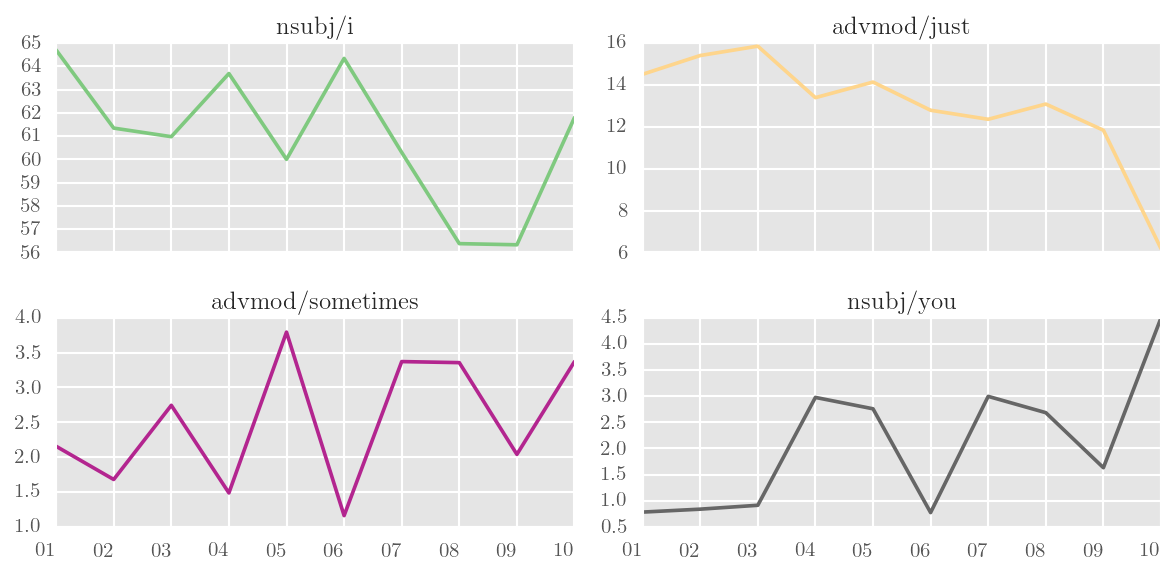
\includegraphics[width=0.70\textwidth]{../images/wonder-example.png}
\caption[Example figure]{Example figure: participants and circumstances for \emph{wonder} as process}
\label{fig:wonder_example_fig}
\end{figure}

\begin{table}[H]
\footnotesize
\begin{tabular}{lrrrr}

\toprule
{} &    nsubj &  advmod &  advmod &  nsubj \\
{} &    i &  just &  sometimes &  you \\
\midrule
01 &  64.705 &  14.509 &  2.156 &  0.784  \\
02 &  61.344 &  15.406 &  1.680 &  0.840  \\
03 &  60.975 &  15.853 &  2.743 &  0.914  \\
04 &  63.690 &  13.392 &  1.488 &  2.976  \\
05 &  60.000 &  14.137 &  3.793 &  2.758  \\
\bottomrule
\end{tabular}
\caption[Example result]{Example result as a multi\hyp{}indexed two dimensional array}
\end{table}

%\begin{minted}[linenos,frame=single,xleftmargin=1cm]{python}
%conc = corpus.concordance(search={GL: doc, F: funcs}, show=[F, L])
%conc.format(n=10, columns=[L, M, R], kind=L)
%\end{minted}

\begin{table}[H]
\footnotesize 
\ttfamily
\begin{tabular}{lrll}

\toprule
0 &                                    &  nsubj\slash i          &  aux\slash be root\slash wonder .\slash , dobj\slash what de \\
1 &                                    &  nsubj\slash i          &  root\slash wonder det\slash the amod\slash same dobj\slash  \\
2 &                                    &  nsubj\slash i          &  aux\slash be advmod\slash just root\slash wonder det\slash  \\
3 &                      nsubj\slash I aux\slash be &  advmod\slash just      &  root\slash wonder det\slash what nsubj\slash person a \\
4 &                                    &  nsubj\slash i          &  root\slash see poss\slash my dobj\slash doc .\slash on prep \\
5 &   nsubj\slash he root\slash say &  nsubj\slash he         &  aux\slash be ccomp\slash wonder mark\slash if nsubj\slash h \\
6 &                                    &  nsubj\slash i          &  aux\slash be root\slash wonder mark\slash if nsubj\slash st \\
7 &                                    &  nsubj\slash i          &  advmod\slash sometimes root\slash wonder mark\slash i \\
8 &                            nsubj\slash I &  advmod\slash sometimes &  root\slash wonder mark\slash if nsubj\slash i aux\slash hav \\
9 &                                    &  nsubj\slash i          &  root\slash wonder mark\slash if nsubj\slash anyone ad \\
\bottomrule
\end{tabular}
\caption[Example concordance]{Example concordance: participants and circumstances in \emph{wonder} process}
\label{conc:wonder_example}
\end{table}

\paragraph{Keywording}

Keywording is a common means of determining which words in a \gls{corpus} are unusually frequent, based on a particular statistical measure such as log\hyp{}likelihood, mutual information or percentage difference (see Section \ref{sect:keywording}). Traditional tools treat keywording as a kind of \gls{corpus} search or interrogation. Keywording is better understood, however, as a statistical operation performed on absolute frequency interrogation results. The new method facilitates using any of these statistical measures in two novel ways. First, keywording is opened up to the full power of the \texttt{search, exclude and show} pipeline. This allows keywording of grammatical participants, or of \gls{POS}\hyp{}lemma pairs. Keywords for n\hyp{}grams, groups and phrases can also be calculated. It becomes possible, therefore, to target particular kinds of constructions, and avoid the use of arbitrary stopword lists. Second, keywords can be calculated in subcorpora using the entire \gls{corpus} as the reference material. This makes it possible to avoid using reference \glspl{corpus}, which are theoretically problematic (See Section \ref{sect:cl-shortcomings}).

\paragraph{Wordlists}

%  (see \texttt{\href{https://github.com/interrogator/corpkit/tree/master/dictionaries}{https://github.com/interrogator/corpkit/tree/master/dictionaries}})
\texttt{corpkit} is designed to be used in tandem with a series of included wordlists. These wordlists were adapted from numerous resources, including the \emph{Process Type Database} \cite{neale_more_2002} and \texttt{pattern.en} \cite{pattern_2012}. This makes it possible to match or remove words of certain types from further analysis. Wordlists include:
%
\begin{enumerate}
\item Closed class words:
\begin{itemize}
\item Pronouns
\item Prepositions
\item Articles
\item Determiners
\item Connectors, conjunctions
\item Modals
\end{itemize}
\item Systemic\hyp{}functional Process Types:\endnote{Original list provided by Mick O'Donnell. Extending these lists to other Process Types is a key future aim.}~
\begin{itemize}
\item Mental
\item Verbal
\item Relational
\item Material
\end{itemize}
\item Conversion\slash normalisation
\begin{itemize}
\item UK\slash US spelling conversion
\item Manual lemmatisation (to augment\slash correct automatic lemmatisation errors)
\end{itemize}
\item Grammar conversion (where possible): from Universal Dependency labels \cite[see][]{nivre_towards_2015} systemic\hyp{}functional labels
\end{enumerate}
%
Each wordlist is a \texttt{Wordlist} object, which has methods for generating verb inflections (via \texttt{WordNet}) or generating regular expressions to match list items:

\begin{minted}[linenos,frame=single,xleftmargin=1cm]{python}
from corpkit.dictionaries.process_types import processes
print(processes.verbal.lemmata[:5])
# ['accede', 'add', 'address', 'admit', 'advise']
print(processes.verbal.words[:5])
# ['accede', 'acceded', 'accedes', 'acceding', 'add']
print(processes.verbal.lemmata[:5].as_regex(boundaries='line'))
# '(?i)^(accede|add|address|admit|advise)$'
\end{minted}
%
Every list can be used as criteria for interrogating \glspl{corpus} or editing results. In the graphical and interpreter interfaces, new wordlists can be interactively created, inflected and saved for later use.

%\subsubsection{Functions}

%\texttt{corpkit}'s core classes and methods are complemented by a number of other functions for saving and loading data, and building regular expressions from wordlists. These are documented online, and in Appendix \ref{appendix:corpkit}.

\paragraph{Additional features}

\texttt{corpkit}'s core classes and methods are complemented by a number of other functions for saving and loading data, and building regular expressions from wordlists. These are documented online, and in Appendix \ref{appendix:corpkit}.

The tool also has broader uses beyond those showcased in this thesis. Language models can be generated from \glspl{corpus}, allowing classification of arbitrary texts by their similarity to texts found in a subcorpus. Such methods make it possible to automatically categorise and interrogate new data. The methods could therefore be applied in near real\hyp{}time to popular online communities, rather than to a community that has completed its lifecycle.

\paragraph{Module dependencies}

\texttt{corpkit} relies heavily on a number of other modules, the most important of which are outlined in Table \ref{tab:corpkit:deps}. Notably, \texttt{Stanford CoreNLP} is used to parse texts, and either \texttt{Tregex} or \texttt{nltk\_tgrep} can be used to query parse trees.\endnote{In this thesis, all constituency queries use \texttt{Tregex}, which has a richer syntax, and is faster.} \texttt{pandas} is another key dependency, being used to store both parser output and search results.

%\texttt{https://github.com/wroberts/nltk_tgrep}

\begin{table}[htb]
\centering
\small
\begin{tabular}{ll}

\toprule
Task                         & Tool  \\ 
\midrule
Tokenisation                 & \texttt{CoreNLP, NLTK} \\     
Lemmatisation (dependencies) & \texttt{Stanford CoreNLP}, \texttt{WordNet} \\
%Lemmatisation (constituencies) & \texttt{NLTK}\slash \texttt{WordNet} \\ 
\gls{XML} manipulation             & \texttt{CoreNLP\_XML}  \\ 
Parse tree traversal         & \texttt{Tregex}, \texttt{nltk\_tgrep}  \\ 
Synonyms, hypernyms, hyponyms & \texttt{NLTK}, \texttt{WordNet}  \\ 
Verb inflections             & \texttt{pattern.en}  \\ 
Linear regression   & \texttt{scipy}          \\ 
Visualisation                & \texttt{matplotlib}, \texttt{pandas}, \texttt{mpld3}  \\ 
Result manipulation          & \texttt{pandas}    \\ 
Multiprocessing              & \texttt{joblib}  \\ 
\bottomrule
\end{tabular}
\caption{Tasks performed in \texttt{corpkit}}

\label{tab:corpkit:deps}
\end{table} 

\subsection{Alternative interfaces}

Though the \gls{API} was used for the analysis of the \glslink{Forum}{Bipolar Forum} \Gls{corpus}, two other inferfaces were also created, in order to maximise the utility of the tool for researchers without expertise in computer programming, or, more specifically, in Python. The first is a graphical application. The second is a natural language interpreter, which parses commands entered by the user and invokes the \gls{API}. These are described in the following two sections.

\subsubsection{Graphical interface}

The simplest of the three developed interfaces is the graphical interface, built using \texttt{Tkinter}. It is reminiscent of other standalone graphical tools such as \texttt{AntConc} and \texttt{UAM Corpus Tool}, providing interfaces for file viewing, corpus searching and concordancing. It extends upon \texttt{AntConc} by adding the ability to parse and search parsed texts, and by allowing the user to work with structured or metadata\hyp{}rich collections of text. It extends on \texttt{UAM Corpus Tool} by providing a greater variety of query languages, as well as result editing and visualisation, and more comprehensive project management, with previous processes stored in memory, so that they may be viewed, saved or discarded. Figure \ref{fig:gui-screenshots} shows the main tabs. Not shown are the \emph{Build} tab (which also visualises parsed sentences), and numerous pop\hyp{}up windows for wordlist creation, thematic category building, and project management.

\begin{figure}[htb]

  \begin{minipage}[b]{0.5\linewidth}
    \centering
    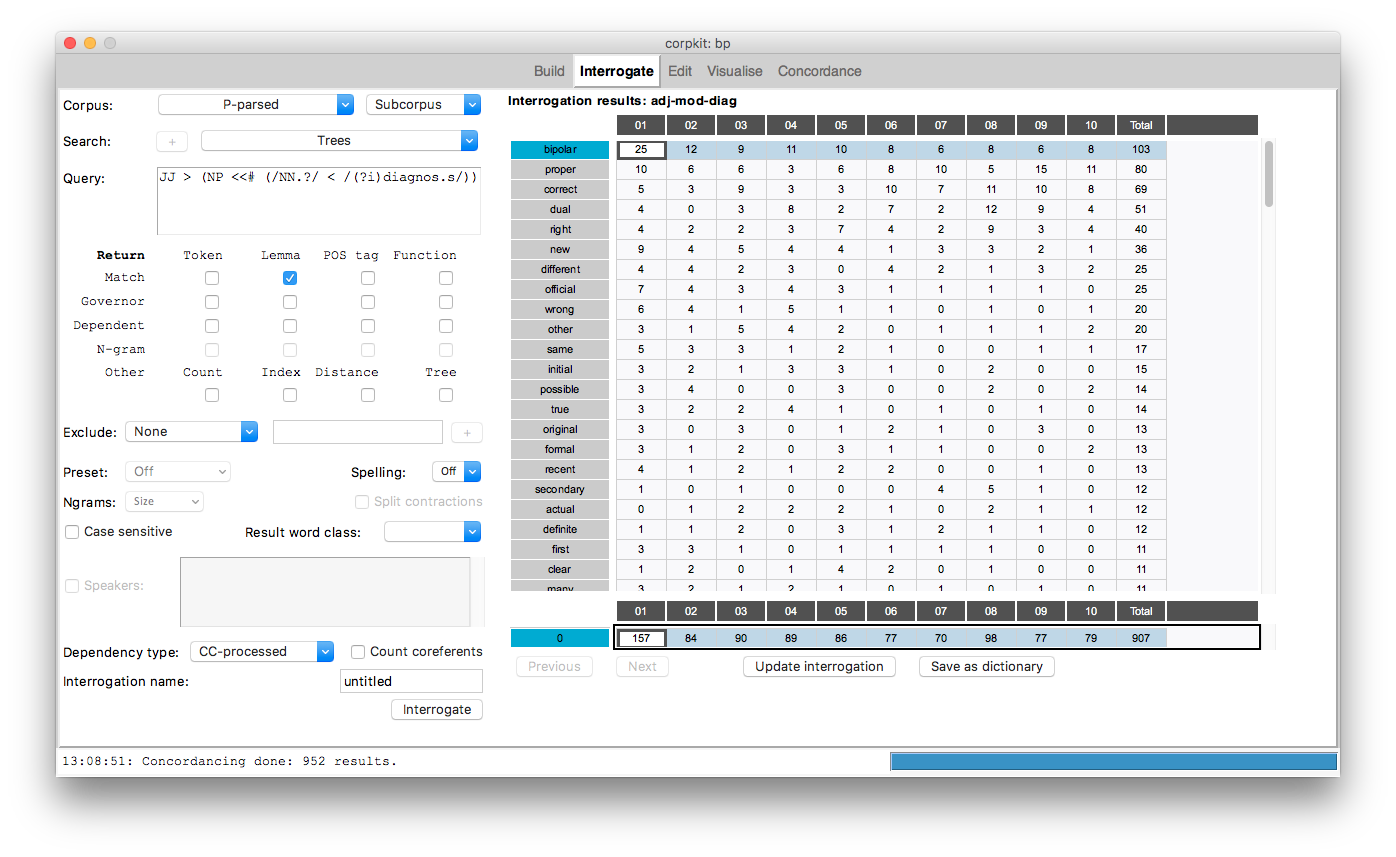
\includegraphics[width=.98\linewidth]{../images/interro} 
    %\caption{Interrogating} 
    \vspace{1ex}
  \end{minipage}%%
  \begin{minipage}[b]{0.5\linewidth}
    \centering
    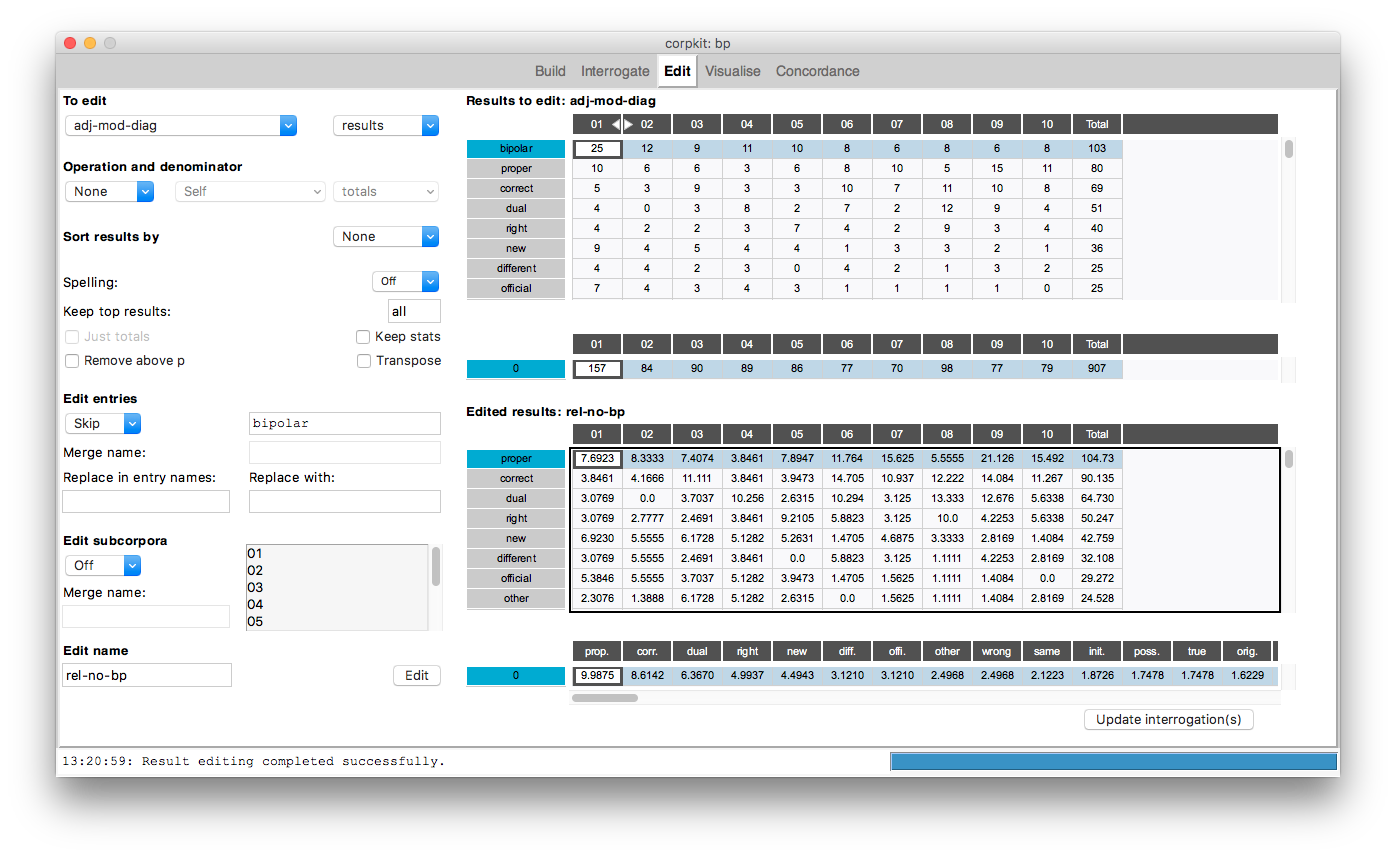
\includegraphics[width=.98\linewidth]{../images/edit} 
    %\caption{Editing} 
    \vspace{1ex}
  \end{minipage} 
  \begin{minipage}[b]{0.5\linewidth}
    \centering
    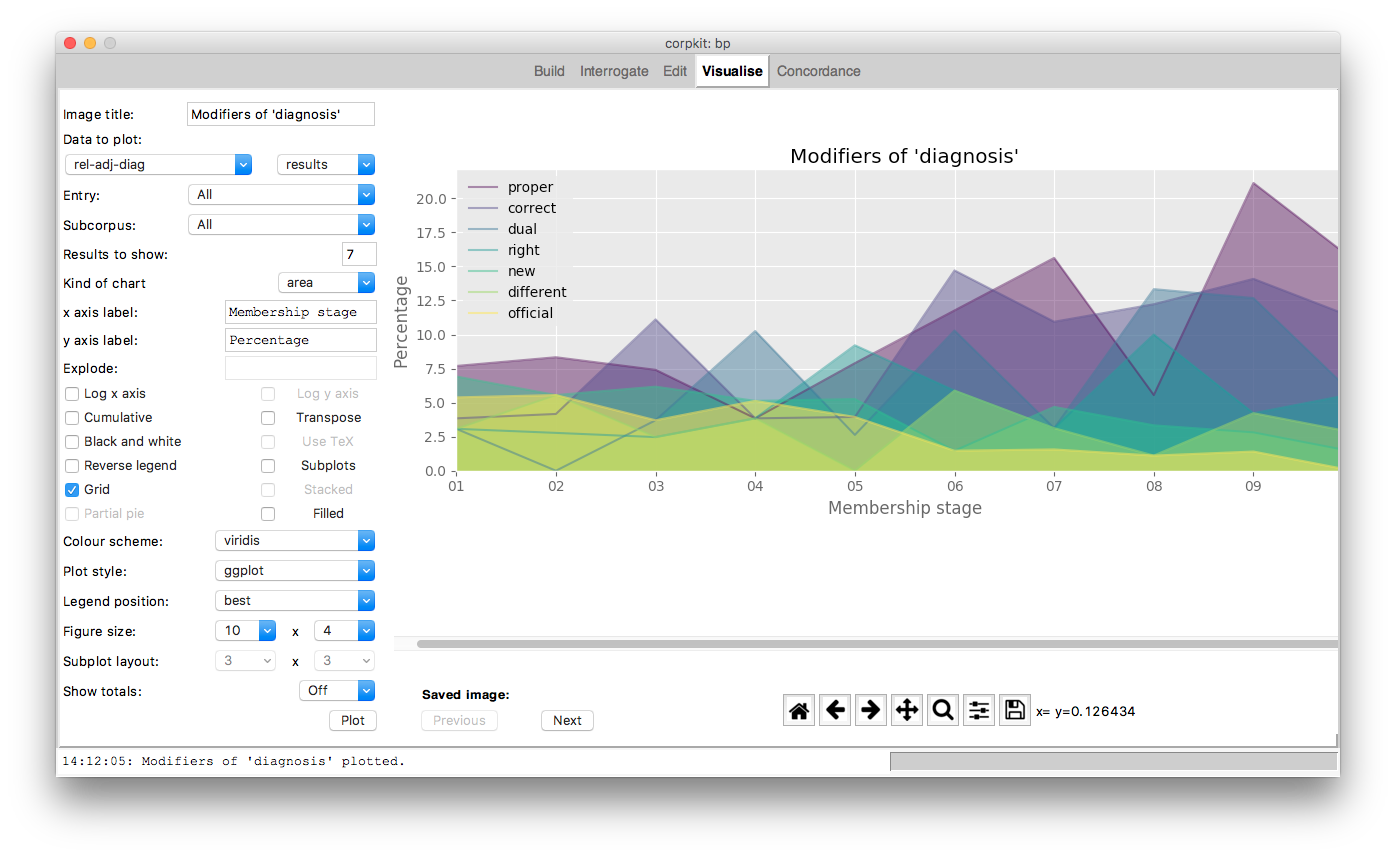
\includegraphics[width=.98\linewidth]{../images/plot} 
    %\caption{Visualising} 
    \vspace{1ex}
  \end{minipage}%% 
  \begin{minipage}[b]{0.5\linewidth}
    \centering
    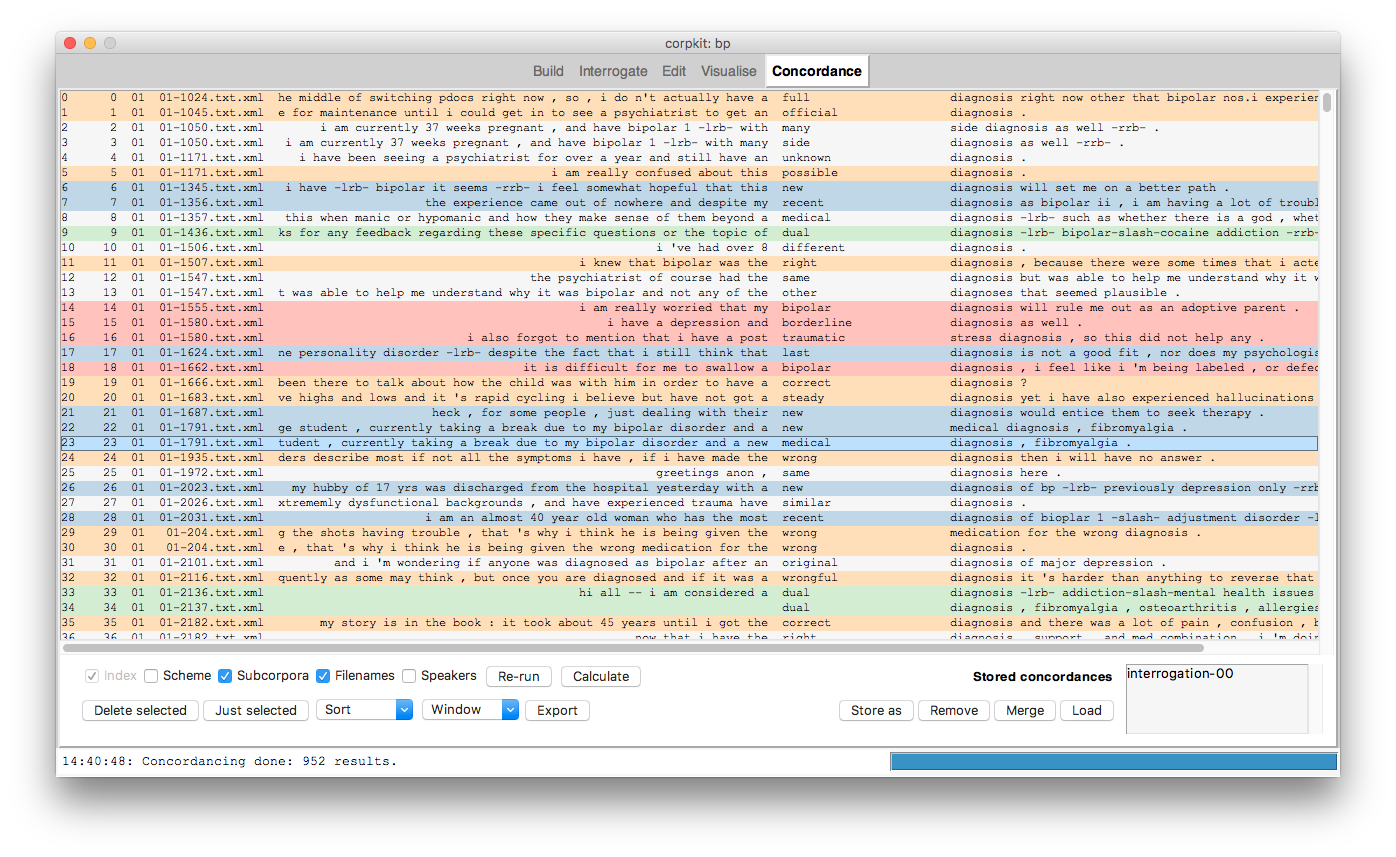
\includegraphics[width=.98\linewidth]{../images/conco} 
    
    \vspace{1ex}
  \end{minipage} 
  \caption{Screenshots from \texttt{corpkit}'s graphical interface}
  \label{fig:gui-screenshots} 
\end{figure}

\subsubsection{Interpreter}

The other alternative interface is a natural language interpreter, which allows the user to type in imperative commands for \texttt{corpkit} to perform. It is reminiscent of the \gls{CWB}. Like the \gls{CWB}, it allows the user to search \glspl{corpus} and annotations in complex ways. The user can create macros and variables, export output, and write scripts that call the tool's functions and methods. It extends upon the functionality of the \gls{CWB} by allowing the user to search fully parsed, rather than \gls{POS}\slash lemmatised text.

\begin{minted}[linenos,frame=single,xleftmargin=1cm,breaklines=true]{bash}
> set bipolar as corpus
> search corpus for governor-lemma matching processes:verbal \
... excluding lemma matching "[write, email, pen]" \
... showing lemma and pos
\end{minted}
%
\noindent The interpreter occupies a middle ground in complexity between the graphical interface and the Python \gls{API}. This makes it particularly suitable as an introduction for corpus linguists to the command line, and programmatic approaches to corpus analysis. Further examples of its syntax can be found throughout Chapter \ref{chap:implications}.

\subsection{Open source development}

A key limitation in previously available \gls{CL} tools addressed by \texttt{corpkit} is in the manner in the tool is provided to the community. In terms of existing \gls{CL} tool, it is notable that most do not provide the end\hyp{}user with access to the source code. At the same time, many are maintained by a single developer. This creates a number of potential problems. First, the software can potentially become a \emph{black box}, where researchers feed in data and interpret output, without understanding what has been done to their data, or how the output was extracted from the input. This can be more or less benign, as when a developer has simply not documented the workings of a feature. At worst, however, the tool may mask its own shortcomings, or remove results that may be important, but apparently uninteresting, or contrary to intuition. At the same time, in closed\hyp{}source software deployment, software users can report, but not fix bugs themselves. This slows down the process of improving a tool, especially in cases where the software is single\hyp{}authored. The second issue that arises in single\hyp{}author, closed\hyp{}source software development is what has been referred to as the \emph{bus factor}, which measures \emph{how many people would need to be hit by a bus in order to make a project unable to proceed?} \cite{cosentino2015assessing}. For many users, switching tools takes significant effort, and involves a learning curve. Making this investment for a tool with an uncertain future may be undesirable. \texttt{corpkit} addresses these problems by being completely open\hyp{}source. Users can not only report bugs, but also fix them. Users may also extend the tool to meet their needs, and request that a developed extension be merged into the master version of the tool. The tool can therefore respond to community needs in a more organic way.

\subsection{Contributions of the toolkit}

The toolkit is a contribution to the \gls{CL} and \gls{SFL} communities, as well as the digital humanities more broadly. It expands on the functionality of many currently available tools, allowing more sophisticated kinds of querying and manipulation than other tools to date. As an example, by allowing the user to forgo reference \glspl{corpus} and stopword lists, its approach to keywording resolves tensions between theoretical orientation of critical\slash functional linguistics (which tend to problematise the notion of balanced\slash representative texts) and keywording (which typically relies on frequency data drawn from reference \glspl{corpus}). \texttt{corpkit} also brings tasks that have typically fallen under the domain of computational linguistics (e.g. lemmatisation, normalisation, parsing, linear regression modelling) to researchers interested in discourse. Despite the notable opposition to lemmatisation and parsing \textcite[by e.g.][]{sinclair_trust_2004}, such perspectives are now uncommon, with increasing recognition that computational methods can enhance the nuance with which the \gls{lexicogrammar} of texts can be probed, and thus the certainty with which claims about \glspl{discourse-semantic} of texts in \glspl{corpus} can be made. Looking at the tool from a computational linguistic perspective, it serves to bring state\hyp{}of\hyp{}the\hyp{}art developments to a new user base, including corpus linguists and discourse analysts. This addresses a problem articulated by \citeauthor{de2008stanford}:

\begin{quote} \singlespacing \small
A major problem for the natural language processing (\gls{NLP}) community is how to make the very impressive and practical technology which has been developed over the last two decades approachable to and usable by everyone who has text understanding need. \dots~ That is, usable not only by computational linguists, but also by the computer science community more generally and by all sorts of information professionals including biologists, medical researchers, political scientists, law firms, business and market analysts, etc. \dots [T]he availability of high quality, easy\hyp{}to\hyp{}use (and preferably free) tools is essential for driving broader use of \gls{NLP} tools \parencite*[p.~1]{de2008stanford}.
\end{quote}

Finally, \texttt{corpkit} is aligned with the emerging areas of digital and programmatic humanities research. It increases transparency and reproducibility of methods and findings: \texttt{Jupyter Notebooks} can be kept under version control and easily shared with others; the graphical interface stores interrogations and edited results in memory during each session, and allows for saving and loading of generated data between sessions. In being free, open\hyp{}source and publicly available, it can be adapted by other researchers, simplifying the process of extending previous research and generating new theory.

\section{Approach to data analysis}

The process of data analysis follows on from the affordances of the developed tools, and from the output of the parsing pipeline: each subcorpus is interrogated via both constituency and dependency parses; results are edited, sorted or merged where necessary to translate findings into meaningful systemic\hyp{}functional terms (insofar as is possible). These findings are then visualised or presented as tables; key points of interest then become the focus of further interrogations. Concordancing and plain-text examples is used where necessary to better understand a given \glslink{lexicogrammar}{lexicogrammatical} phenomenon in co\hyp{}text. As the key area of interest is longitudinal change, linear regression is performed on many interrogation results to calculate trends. This is followed by sorting of the entries by slope, in order to unearth parts of the lexicogrammar that become more or less frequent over time, are turbulent, or remain static.

The approach to analysis can be characterised as \emph{systematic}, \emph{exploratory} and \emph{recursive}:

\subsubsection*{Systematic progression through data}

Interrogation progresses along the cline of instantiation, from broad\slash shallow features to more specific \glslink{lexicogrammar}{lexicogrammatical} realisations. Where possible, investigation of \sctext{Mood} and \sctext{Transitivity} features are also interrogated separately. This `from\hyp{}above' approach is unusual in automatic analysis of text \cite{matthiessen_key_2010}; it is made possible by the combination of full parsing, which gives access to broad features, and the use of theory, which allows targeting expected linguistic sites of change.

\subsubsection*{Exploratory components}

Given the fact that \texttt{corpkit} allows rapid interrogation of the dataset, testing hypotheses is often trivial. As such, features of the \gls{lexicogrammar} that are not expected to be particularly salient (change in determiner use over time, for example) can be tabulated nonetheless. Much of the work of the analysis consists of iteratively exploring the \gls{corpus}, guided by the findings of previous investigations: If past tense appears to be a key feature undergoing longitudinal change, a follow\hyp{}up investigation may count Predicators in past tensed clauses, or look for keywords in these clauses' Adjuncts.

\subsubsection*{Recursivity}

Programmatic methods simplify and expedite the process of querying large datasets. As such, a great deal of recursivity is possible. For example, code can be written that locates key heads of Participants in the \gls{corpus}, searches for processes in which these words are Participants, and so forth. This kind of interrogation was occasionally performed, and is for the most part documented in the accompanying Notebook, rather than in the findings section, as description of methodological steps is unwieldy, compared to simply reviewing\slash rerunning the code.

\subsection{\texttt{IPython} \& the \texttt{Jupyter Notebook}}

\texttt{IPython} is an extension of the Python programming language, designed to allow quick access to Shell commands, to store code output to file and to easily access the output of previous commands \cite{perez2007ipython}. \texttt{Jupyter Notebooks} are web browser based displays of \texttt{IPython} code, as well as code output, headings, text, and multimedia. \texttt{Jupyter Notebooks} are increasingly popular within scientific communities, as they allow code to be contextualised and explained multimodally, and can be easily run by other researchers, ensuring reproducibility of results. Much of the corpus investigation took place via \texttt{IPython} and \texttt{Jupyter Notebooks}. Many key findings from the investigation in this thesis are therefore available in Notebooks available at: \texttt{\href{https://github.com/interrogator/thesis}{https://github.com/interrogator/thesis}}. This Notebook presents methodological processes and code in more depth, and can be used to manipulate the \gls{corpus}, and edit findings and results.

\subsection{Limitations}

The methodology has some limitations. First, it is bound by the speed and accuracy of its dependencies, with shortcomings of other tools inherited into every investigation. Second, it is strongly oriented toward quantitative insights into \gls{corpus} texts, at times homogenising data prior to analysis. This means that bottom\hyp{}up, grounded\hyp{}theory\hyp{}based interpretation of the dataset is not always possible. As such, the emergence of theory from data is perhaps less likely. The methodology also relies on ad\hyp{}hoc translation between three grammars of English---constituency, dependency and the \gls{SFG}. This means that linguistic notions may be simplified, and categories conflated when distinctions are not shared by all grammars. A further consequence is that it is not possible to engage deeply with concepts in \gls{SFL}\slash \gls{SFG} that make it a particularly attractive framework for locating \gls{discourse-semantic} phenomena at risk in a structured \gls{corpus}.

Second, the methodology is also based on relatively simplistic statistical methods. Though the output of interrogations is amenable to complex statistical analysis, here, most results are generated via simple relative frequency or keyness calculation, ordered using least\hyp{}squares regression. This precludes, for instance, predictive applications of the methods, which could reveal which members are likely to progress to veteran stages, or to drop out.

Finally, the methodology is limited to querying the annotated data, and manipulating results. Though strategies for querying the data are more complex than is typical of \gls{CL}\slash \gls{CADS} research, the methodology does not harness a number of emerging methods in computational linguistics for categorising and understanding the content and context of digitised texts. Machine learning approaches to text analysis, for example, allow unsupervised classification of documents based on automatically determined features that theoretically motivated human researchers may not consider. The need for later research to apply state\hyp{}of\hyp{}the\hyp{}art computational techniques is described in Chapter \ref{chap:implications}.

%The complementarity of methods from computational linguistics and discourse analysis is discussed in more detail in Chapter \ref{chap:futuredirections}.

%Topic modelling\endnote{Exploratory topic modelling of the \gls{Forum} contents was performed, using \sctext{Mallet}; spatial considerations prevented the analysis from being presented in this thesis, however.} can be used to automatically group corpus texts by semantic field, based on co-occurrence of lexical items. 

\section{Situating the thesis methodology}

The methods outlined here incorporate components from a number of convergent fields of study, such as text mining, \glslink{CL}{corpus linguistics}, computational linguistics, and the digital humanities. There is no clear line delineating where one of these fields ends and another begins. There is, however, a tendency for digital humanities and \gls{CL} to focus on interpreting specific datasets, while text mining and computational linguistics are primarily interested in the development of tools. A mixed emphasis on methodological innovation and data analysis means that the case study straddles a broad interdisciplinary space. For discourse analysts and corpus linguists, the methods present new ways to engage with well\hyp{}established computational linguistic practices and tools, allowing automatation of work that has previously been possible only through manual analysis. At the same time, text mining and computational linguistics are often concerned with extracting entities and entity relationships, with little consideration of grammatical metaphor, or theories of language and grammar more generally. The developed method thus aims to combine the speed and automation of text mining approaches with the grammatical sensitivity seen in qualitative research. This opens up future research agendas that integrate discourse analysis and state\hyp{}of\hyp{}the\hyp{}art computational linguistic methods.

\section{Chapter summary}

In this chapter, I have outlined and justified the elements of the data collection, approach to analysis and tool development. The following chapters operationalise the methodology in order to investigate language features in the \glslink{forum}{Bipolar Forum}. The analyses is followed by a discussion of findings in Chapter \ref{chap:discuss-bp}.


% why socialisation

%Socialisation is preferred here because it aligns with the systemic\hyp{}functional notion of interaction as interpersonal exchange, with \sctext{Mood} system choices realising an ongoing negotiation of speaker roles. Like \gls{SFL}, socialisation research tends to eschew the cognitive and psychological 

%Because the case study of this thesis does not involve interviews with participants, or any demographic information beyond what is available to all \glspl{member} of the \gls{Forum}, 

%As discussed in Chapter \ref{chap:discussion}, understanding the underlying cause of change is not a prerequisite to modelling or predicting it.

%!TEX root = ../thesis.tex

\chapter{An introduction to the data: generic features of the Forum} \label{chap:introdata}

In the previous chapters, I described the context, theoretical background and potential approaches of a case study designed to understand longitudinal change in language use in \emph{\glslink{Forum}{Bipolar Forum}}, a \gls{bipolar} \gls{OSG}. In this and the next two chapters, I present the finding of the case study. The Bipolar Forum Corpus, and its Membership Stage Structure representing ten stages of membership, is the main dataset used. This chapter provides an introduction to the \gls{corpus} from both qualitative and quantitative perspectives. First, I present a genre analysis of a small selection of \glspl{post}, which highlights text structure beyond the level of the clause, and familiarises the reader with the kinds of language in the \gls{corpus}. This is followed by a presentation of shallow quantitative features in the \gls{corpus}' ten subcorpora. Chapter \ref{chap:interpersonal} contains findings from the \sctext{Mood} and \sctext{Modality} analysis. Chapter \ref{chap:experiential} contains findings from the \sctext{Transitivity} analysis.

%todo: tense?
%todo: copy edit
The case study was data\hyp{}driven and exploratory: results from one interrogation could largely determine what next needs to be explored. At other times, it was driven by the results of prior studies of language use in \glspl{OSG}, in communities generally, and in healthcare institutional settings. It is also theoretically informed, based on relationships between \gls{lexicogrammar} and meaning provided by \gls{SFL}. In this and the following two chapters, therefore, findings are generally accompanied by a brief discussion of their \gls{discourse-semantic} significance. There are two reasons for this structural choice. First, because the analysis was exploratory, with more delicate querying following broader querying, \glspl{discourse-semantic} needed to be presented \emph{in situ} in order to justify movement from one component of the \gls{lexicogrammar} to the next. Analysis of \glspl{discourse-semantic} was an integral part of the research process as it unfolded, rather than a task to be undertaken after the investigation had concluded. Second, the co\hyp{}presentation of wordings and their meanings more closely models the way humans use and understand language: it makes little sense to keep discussion of meaning separate from discussion of wording, as readers naturally interpret the meaning behind wordings as they encounter them.

Accompanying these chapters is a series of \texttt{Jupyter Notebooks}, containing the figures and concordance lines presented here, as well as the code used to generate them. They also document the functionality of \texttt{corpkit}, the toolkit used for analysis, in more detail, provide further examples from the auxiliary \glspl{corpus}, and document raw findings (i.e. frequency tables, etc.) that cannot be included in this chapter for reasons of space. The Notebooks are designed to facilitate reproducibility and transparency, and allow easy future applications of methods developed here to new datasets. They can be accessed via \texttt{GitHub} at \texttt{\href{https://github.com/interrogator/thesis}{https://github.com/interrogator/thesis}}.

\section{Genre and first contributions}

Though the case study analysis is for the most part a quantitative, computational one, the analysis begins with a qualitative, genre\hyp{}oriented analysis of some individual \glslink{post}{contributions} to the \gls{Forum}. I unpack generic features of a small selection of first \glspl{post} and replies they receive, using the approach to genre analysis outlined by \textcite{eggins_analysing_2004} and reviewed in Section \ref{sect:sfl}.
%This section is not intended to be an in-depth investigation of genre. Instead, it is intended to demonstrate that language choices in the community are affected by contextual parameters that are difficult to locate automatically. This is argued to be a major challenge of automatic discourse analysis in Chapters 7 and 8.
Foregrounding the qualitative analysis serves two main purposes. First, it provides a context for the abstracted \glslink{lexicogrammar}{lexicogrammatical} findings that follow: before analysing a \gls{corpus}, it makes sense for the researcher to have familiarised him\slash herself with some of its texts. Second, it foregrounds limitations inherent to the automated, computational searching of the \gls{corpus}. Contributions to the \gls{Forum} follow generic constraints---these, however, are not considered during automated searching. Later chapters discuss this problem, and potential solutions, in greater detail.

%todo: copy edit
One particular \gls{thread}, entitled `\textbf{am i bipolar and what should i do?}' is analysed in more detail than others. It is comprised of a new \glslink{member}{user}'s first \gls{post}, and replies from existing \glspl{member}. It was chosen because it contained \glspl{post} from \glslink{member}{users} spread across the ten stages of membership, and because it contained discussion of key social actors in the Field of discourse, such as friends and family and health professionals. Based on simple reading of \gls{Forum} \glspl{thread}, it also appeared to be relatively typical in terms of length, content and participating users.%
\endnote{The qualitative, generic analysis was in fact undertaken as a kind of pilot study, before any corpus linguistic analysis was performed. The \gls{thread} selected for analysis was therefore not chosen because it exemplified quantitatively identified features. The fact that many phenomena identified during the qualitative analysis are picked up during the \gls{corpus} analysis is not by design---rather, it highlights the surprising uniformity of texts within the genre of `first post threads'.}

\subsection{A user's first contribution to the Forum} \label{sect:jess-post}

% amylb1990400
On May 30, 2011, jessff1989787, a 20 year old female from England, \glslink{post}{posted} a new \gls{thread}, `\textbf{am i bipolar and what should i do?}', to the \glslink{Forum}{board}:

\begin{quote}
\resetlinenumber
\footnotesize{
\singlespacing{
\begin{linenumbers}
\begin{verbatim}
hi im jess new to this site, umm... well im currently 20 years 
old and have been diagnosed with depression from a young age 
but in the last 5 years or so i have been feeling very odd having 
some extreme highs which include loss of appetite concentration
using drugs and alcohol spending sprees and also sex, i can not 
control this when i get impulses like the above it is impossible 
though i have tried. I also suffer with depression which is quite
severe most of the time i find it hard to get out of bed or to 
even be able to connect with anyone including my partner who 
lives with me, i am hurting him so much but i dont feel like i 
can do anytjing about it
    i have asked my doctor to test me to see if i am bipolar as my 
antidepressants do not work even though they have been changed a 
million times!! he said no that he wont test me and i also asked 
for counselling and he also declined that, at the moment i feel 
that im loosing control of everything and its getting worse, i 
want to change my doctor and have been telling my partner i would 
but im scared of finding out that i am bipolar, but i really feel 
like either an extreme high or an extreme low is on the way and 
im quite scared i dont know what to do
    please help \end{verbatim}
\end{linenumbers}
}}
\end{quote}

%The text and its purposes are typical of newcomers' first \glspl{post} to an \gls{OSG}:
The \gls{post} is reminiscent in form and function to \glspl{post} analysed in other work on \gls{OSG}: Jess indicates a need for general social support (\emph{im quite scared}, line 20) and requests advice (\emph{what should i do?}, title; \emph{i dont know what to do}, line 21). As noted by \textcite{smithson_developing_2012} and \textcite{varga2014grieving}, in order to legitimate herself as a potential \gls{member}, and add perlocutionary force to her request, Jess also offers a narrative designed to demonstrate that she likely suffers from \gls{bipolar}, and thus fulfills the membership criteria of the \glslink{Forum}{board}. Also notable is the sense of urgency, which has been conveyed through an apparent lack of planning within the post, spelling errors (\emph{anytjing}, line 11; \emph{loosing control}, line 17), and the pervasive joining of clauses through conjunction. As noted by \textcite{horne_doing_2009}, this may be a strategy for increasing the likelihood of response. In the context of bipolar disorder, it could also connote the onset of a manic episode, which would serve to bolster the claim to membership.

\subsubsection{Generic stages in Jess first post}

The \gls{post} appears to borrow from both \sctext{self\hyp{}introduction} and \sctext{narrative} genres identified by \textcite{labov_narrative_1997}. Indeed, in many ways, the \gls{post} conforms to the \sctext{narrative} genre, which has the structure:

\begin{quote}
(Abstract) $\hat{}$ Orientation $\hat{}$ Complication $\hat{}$ Evaluation $\hat{}$ Resolution $\hat{}$ (Coda)
\end{quote}

\noindent where

\begin{itemize}\onehalfspacing{
\item \sctext{Abstract} is an encapsulation of the point of the story
\item \sctext{Orientation} orients the listener to the circumstances of the story
\item \sctext{Complication} is temporally sequenced event which culminates in a problem
\item \sctext{Evaluation} is the attitude of the speaker toward the \sctext{complication}
\item \sctext{Resolution} is how the story's protagonist resolved the \sctext{complication}
\item \sctext{Coda} makes a point about the text and may reorient the listener to the present \cite[p.~32]{labov_narrative_1997}.
}
\end{itemize}
%
The \sctext{abstract} stage is realised by the \gls{post}'s title; \sctext{orientation}, \sctext{complication} and \sctext{evaluation} do follow, though they appear to be recursive. Also different is the focus of the \sctext{evaluation}: here, it refers to an \sctext{evaluation} of the previous complication, rather than an evaluation of the narrative itself. The most significant deviation is that rather than a \sctext{resolution} (and optional \sctext{coda}), there is a \sctext{request} to other members for `help', presumably with the questions \glslink{post}{posted} in the title: whether or not she is bipolar, and how she should respond to her presented self\hyp{}evaluation.

\begin{table}[htb]\centering\small
\begin{tabularx}{\textwidth}{lX}

\toprule
Genre stage  & Sentences in Jess's first\hyp{}\gls{post}   \\ \midrule
\sctext{Abstract }    & am i bipolar and what should i do? \\ 
\sctext{Salutation}   & hi im jess   \\ 
\sctext{Orientation}  & (I am) new to this site,  umm... well im currently 20 years old and (I) have been diagnosed with depression from a young age but \\ 
\sctext{Complication (1)} & in the last 5 years or so i have been feeling very odd, (I have been) having some extreme highs which include loss of appetite concentration using drugs and alcohol spending sprees and also sex, \\ 
\sctext{Evaluation (1)}   & i can not control this when i get impulses like the above it is impossible though i have tried \\ 
\sctext{Complication (2)} & I also suffer with depression which is quite severe most of the time i find it hard to get out of bed or to even be able to connect with anyone including my partner who lives with me,   \\ 
\sctext{Evaluation (2)}   &  i am hurting him so much but i dont feel like i can do anytjing about it   \\ 
\sctext{Complication (3)} & i have asked my doctor to test me to see if i am bipolar as my antidepressants do not work even though they have been changed a million times!! he said no that he wont test me and i also asked for counselling and he also declined that, \\ 
\sctext{Evaluation (3)} & at the moment i feel that im loosing control of everything and its getting worse, \\ 
\sctext{Complication (4)} &  i want to change my doctor and (I) have been telling my partner i would but im scared of finding out that i am bipolar, but  \\ 
\sctext{Evaluation (4)}   & i really feel like either an extreme high or an extreme low is on the way and im quite scared i dont know what to do  \\ 
\sctext{Request}     & please help   \\ \bottomrule
\end{tabularx}
\caption{Genre stages in Jess's post}
\end{table}
%
Within a possible `first\hyp{}\gls{post} genre', explicit \sctext{Requests} are potentially optional \cite{vayreda_social_2009}, though other members may interpret descriptions of problems and the act of posting themselves as warranting the provision of advice \cite{goldsmith2000soliciting}. Others \cite[e.g. ][]{herring_two_1996,weber_missed_2011} have noted that \glslink{member}{users} may not begin introductions to online communities with an explicit \sctext{salutation}: as all messages are attributed to the writer's username multimodally, and even new \glslink{member}{users} are likely familiar with the way in which the site presents \glspl{post}, \sctext{salutation}, if not rendered explicitly in prose, is in some sense embedded within the architecture of the \gls{forum} \gls{mode} itself. Given that all \glspl{post} must be titled, and that titles almost always summarise the content of the \gls{post}, \sctext{Abstract} is an obligatory stage. The generic structure provided by \textcite{labov_narrative_1997} could thus be adapted for this case as:

\begin{quotation}\small
\noindent Abstract $\hat{}$ Salutation $\hat{}$ Orientation $\hat{}$ [ Complication $\hat{}$ Evaluation ]\textsuperscript{n} $\hat{}$ (Request)
\end{quotation}
%
To characterise the extent to which Jess's post was representative of the genre, the two first \glspl{post} with the smallest wordcount were located and a basic genre stage analysis was performed (Table \ref{tab:two-genre-stage-analyses}). It was assumed that small first \glspl{post} would contain only obligatory genre features. These short \glspl{post} indicate that \sctext{evaluation} is an optional stage, and confirm that recursion of \sctext{complication} and \sctext{evaluation} is optional (though perhaps a key feature in developing a sense of urgency). \emph{Short Post B} shows that the optional \sctext{coda} noted by \textcite{labov_narrative_1997} appears to be possible within the first\hyp{}\gls{post} genre. This leaves a finalised generic structure for \gls{thread}\hyp{}initial first \glspl{post} within the \glslink{Forum}{Bipolar Forum}:

\begin{quotation}\small
\noindent Abstract $\hat{}$ Salutation $\hat{}$ Orientation $\hat{}$ [ Complication $\hat{}$ (Evaluation) ]\textsuperscript{n} $\hat{}$ (Request) $\hat{}$ (Coda)
\end{quotation}

\begin{table}[htb]
\small\centering
\begin{tabularx}{\textwidth}{lXX}
\toprule
Genre stage  & Sentences in Short Post A  & Sentences in Short Post B \\ \midrule
\sctext{Abstract}     & \emph{Lamictal}  & \emph{Depakote and hair thinning - any suggestions?}  \\
\sctext{Salutation}   & Hi-                                                                              & Hi                                                                      \\
\sctext{Orientation}  & I'm on my 3rd day of Lamictal and                                                & My daughter has been on Depakote for 4 months and                       \\
\sctext{Complication} & it's giving me weird almost headache like pains in my head                       & (she) has experienced some (h)air thinning                              \\
\sctext{Evaluation}   & ~                                                                                & ~                                                                       \\
\sctext{Request }     & Has anyone else had this happen while taking lamictal and when does it go away? & Has anyone out there found an effective way to counteract this problem? \\
\sctext{Coda}         & ~                                                                                & She is on 500mg per day. Any suggestions really appreciated.            \\
\bottomrule
\end{tabularx}
\caption{Genre stages in short first contributions}
\label{tab:two-genre-stage-analyses}
\end{table}
%
It is not enough, however, to simply look at the features of the \gls{post}: as \textcite{eggins_analysing_2004} explain, perhaps the best indicator of genre conformity is the way in which other members respond to the presented text. Thus, at this point, the investigation turns to consider replies to Jess's first \gls{post}.

\subsection{Replies to a first post}

Jess's first \glslink{post}{contribution} received six replies over the course of seven hours, from \glspl{member} with post counts ranging from five to over 5,000. Due to limitations of scope, only two of these replies have been selected for further analysis. They were selected based on the post count of the writer at the time of posting: one is a newer user (Subcorpus 03) and the other is a very senior member (Subcorpus 10). They also bookend the replies: the newer user is the first to respond to Jess, and the veteran member the last. The qualitative analysis, therefore, provides a description of language use at multiple stages of the membership course. The complete \gls{thread}, including the other four replies, is available in Appendix \ref{appendix:thread}.

The first reply was a response from \emph{Luvsoccer}, who had a total of five \glspl{post} to the \glslink{Forum}{board}:

\begin{quote}
\resetlinenumber
\footnotesize{
\singlespacing{
\begin{linenumbers}
\begin{verbatim}
It sounds like you might have bipolar to me. You need to change 
Drs. One with more knowledge apparently. The reason the 
antidepessants are not Working is because If you are bi polar 
and they put U on an antidepressant alone it can make things 
worse... I know from experience. Don't be scared it's treatable. 
Find you a dr that can make a correct Diagnosis and go from there. 
Good luck! \end{verbatim}
\end{linenumbers}
}}
\end{quote}
%
\noindent Following \emph{Luvsoccer} were four replies from other \glspl{member} at differing membership stages, unanalysed here. The final \gls{post} in the \gls{thread} was by \emph{Emz45}, who at the time of data collection had authored 5071 \glspl{post}:

\begin{quote}
\resetlinenumber
\footnotesize{
\singlespacing{
\begin{linenumbers}
\begin{verbatim}
Hi, welcome to the boards, hopefully we can help you out and be 
a support system for you. First off you're not A bipolar, *l* 
we're not things, it's a condition. From what you say, if 
sounds very likely that you might have Bipolar disoder. I would 
go to a psychiatrist for testing and find out. You don't have to 
have your docs permission to do this. If you're already seeing a 
psychiatrist and that's who's doing all the denying, then find a 
different one, because he's not doing his job, nor is he 
considering your best interest. That's all that you can really 
do in the beginning, find out what's what. We aren't docs here 
and can't diagnose you. But I think it would definitely be smart 
to go and get a diagnoses.

Take care, and please keep in touch, let us know how you're 
doing, okay?

Kat \end{verbatim}
\end{linenumbers}
}}
\end{quote}
%
\noindent The original poster did not contribute to the \gls{thread} again, but \glslink{post}{posted} to the \glslink{Forum}{board} on three other occasions in the next week, interacting again with \emph{Emz45}.

\subsubsection{Analysis of replies} \label{sect:qual-reply-analysis}

A first notable feature of the replies is their functional similarity. Both Luvsoccer and Emz45 offer social support (\emph{Don't be scared}, line 5; \emph{take care}, line 14), and encourage Jess to find a new doctor. Both also hint at a likely diagnosis based on the symptoms she has presented. In both cases, key ideological tenets of the \gls{Forum} are represented delicately. Both disparage the work of Jess's current psychiatrist (\emph{One with more knowledge}, line 2; \emph{he's not doing his job}, line 8). Both navigate the \gls{Forum}'s conflict between an inability to provide official diagnoses and an orientation toward supporting those who appear to have \gls{bipolar}. In fact, both provide near\hyp{}identical wordings:

\begin{enumerate}
\item \emph{It sounds like you might have bipolar to me}
\item \emph{From what you say, if sounds very likely that you might have Bipolar disoder}
\end{enumerate}
%
Both statements essentially amount to a lay diagnoses, with modulation, modalisation, embedding and dummy Subjects used to reduce certainty and to avoid attribution of the diagnosis to the speaker herself. Both further hedge the lay diagnosis by stressing the need for a professional diagnosis, and, in doing so, deny that what they offered was any kind of diagnosis at all.

%todo: first sentence doesn't make sense
The relationship between first\hyp{}\gls{post} and reply differ across the hierarchy of stratification. At the stratum of genre, unlike first \glspl{post}, the two replies do not conform rigourously to an identifiable sequence of clause functions. At the same time, the fact that the two responses overlap in content may be a useful indication that first \glspl{post} do constitute a genre that is recognised by other \glspl{member} of the \glslink{Forum}{community}. In terms of register, while the dimension of Field remains largely consistent (aside from Emz's avoidance of the topic of specific medications), the most dramatic differences are within Tenor: Jess is a prototypical newcomer, describing a medical history and current problem, positioning herself as vulnerable, lacking agency, and unable to participate effectively in her own care. In contrast, to Jess's descriptions of the past and present, Luvsoccer and Emz offer explanations and potential actions for the future. 

Within the \gls{lexicogrammar}, we can see differences in how the first and non\hyp{}first\hyp{}\glspl{post} construe reality via the system of \sctext{Transitivity}. All participants position themselves as Sensers, but the kinds of mental processes vary in their representation of subjectivity, reasoning and control. Jess characterised herself through subjective mental processes over which she has no agency (\emph{i have been feeling very odd}, \emph{i dont feel like i  can do anytjing about it}, \emph{i feel that im loosing control of everything}, \emph{i really feel like either an extreme high or an extreme low is on the way}); Luvsoccer, in contrast, \emph{know[s] from experience}, while Emz \emph{thinks} that diagnosis is the most important next step. Jess construes the health professional as an Agent, and most often, a Sayer (\emph{He said no}; \emph{He also declined that}), whose actions negatively affect her ability to obtain needed treatment. This contrasts with the other members, who reformulate health professionals as Goals (\emph{You need to change Drs}; \emph{Find you a dr}; \emph{I would go to a psychiatrist for testing}, etc.) Jess positions her partner, on the other hand, only as a Goal or Target, and never a Participant that puts processes in motion (\emph{i find it hard to [...] to connect with anyone including my partner}; \emph{i am hurting him so much}; \emph{I ... have been telling my partner}). For this reason, the partner is not construed at all in either response.

%Emz's advice provision strategy is to use modalisd material processes to show Jess the result of her reasoning: in \emph{I would go to a psychiatrist for testing and find out}, Emz foregrounds actions based on her familiarity with the situation.

There are also differences in the way first and non\hyp{}first \glspl{post} instantiate the system of \sctext{Mood}. All of Jess's major Mood choices are declarative and congruently work to provide information, until a final imperative, \emph{please help}, which shifts the function of the \gls{post} from the recursive narrative stages of \sctext{Orientation}, \sctext{Complication} and \sctext{Evaluation}, making a modulated demand on readers to address her declared fear and need for information (\emph{im quite scared i dont know what to do}). The Subject of most of Jess's clauses is \emph{I}, emphasising the self as the one invested with modal responsibility, and thus, the one who will honour any advice that others choose to provide. Modalisation of the self as Subject is used to stress an inability to modify behaviour (\emph{I can not control this}, \emph{I don't feel like I can do anything about it}). This is in contrast to the responses, which use interrogative and imperative Moods to request further information and to command the new user to respond. \emph{You} is by far the the most common Subject in the two replies, as the responses keep modal responsibility on Jess herself. Modalised declarative choices, meanwhile, do not always provide information, but may also issue directives in the form of advice: emz does this twice, casting herself as the hypothetical actor in the first (\emph{I would go to a psychiatrist for testing and find out}) and using rank shifted and non\hyp{}rank shifted modulation strategies to hedge the second (\emph{\textbf{I think} it would \textbf{definitely} be smart to go and get a diagnoses}).

%todo: repeated
Also observable are subtle differences between the two replies, caused primarily by membership stage. Luvsoccer's post is a part of Subcorpus 03; Emz45's is in Subcorpus 10. First, in terms of choices of Field, Luvsoccer attempts to explain the reason that antidepressants are not helping, while Emz avoids the topic completely. This is related to the gradual rise in general offerings of social support and the decrease in references to specific medications \cite{wang_stay_2012}: veteran \glslink{member}{users} may refrain from offering specific advice on medication choice and dosage, as within a normative biomedical ideology, these are domains restricted to the health professional \cite{vayreda_social_2009}. Another key difference between the two replies is in the source of knowledge underlying the advice. Luvsoccer foregrounds personal experience by construing herself as the Senser (\emph{It sounds to me}; \emph{I know from experience}); Emz, on the other hand, only represents herself as a \gls{member} of the \glslink{Forum}{board} (\emph{hopefully we can help you}, \emph{we aren't docs and [we] can't diagnose you}), as the Subject within hypothetical advice (\emph{I would go to a psychiatrist}), and within rank shifted modulation of another advice instance (\emph{I think it would definitely be smart to go and get a diagnoses}). 

A third notable difference is in the ways the two replies are concluded. After offering advice, Luvsoccer simply writes \emph{Good luck!}, effectively signalling the end of her part in the interaction. Emz, on the other hand, attempts to maintain dialogue (\emph{please keep in touch, let us know how you're 
doing, okay?}) by commanding the user to report back, hedging through the use of a tag question seeking agreement\slash permission. Emz's conclusion opens up space for further exchange within a community where all interpersonal exchange is understood to contribute to wellbeing.\endnote{This can also be seen as an attempt to maintain active discussion within the forum more generally: veteran members contribute by choice, and are therefore personally invested in the health of the community itself.}

Emz45's reply also shows us that veterans' preference for jargonisation is not absolute. Here, presumably because she is interacting with a new \glslink{member}{user}, she opts for lay terms (\emph{bipolar disoder}, \emph{psychiatrist}, \emph{diagnoses}). This contrasts with Luvsoccer, who uses the developing shorthand forms for health professionals (\emph{dr}, \emph{drs}), but not the jargonised variants that distinguish between particular kinds of health professional.

A final important difference between the two replies is the way in which they advocate changing doctors\slash psychiatrists. Compare:

\begin{multicols}{2}
\begin{quote}
\sctext{Luvsoccer}

\emph{You need to change Drs. One with more knowledge apparently.} ~\\~\\~\\
\end{quote}

\begin{quote}
\sctext{Emz45}

\emph{If you're already seeing a psychiatrist and that's who's doing all the denying, then find a different one, because he's not doing his job, nor is he considering your best interest}
\end{quote}
\end{multicols}
%
\noindent Though Emz is by far the more senior member, her advice is conditional, and sensitive to an ambiguity concerning the type of health professional Jess is currently seeing. Emz is also the only one who provides an explicit reason for the need to change. Luvsoccer's reasoning must be inferred from the statement that the doctor lacks knowledge, and has prescribed what she believes to be inappropriate medication. 

%Notably, Luvsoccer's reply is ignored by Emz, despite a great deal of overlap in content. This too hints at the generic nature of first \glslink{post}{contributions}: unlike non-first\hyp{}\gls{post} threads, first \glspl{post} are not many-to-many discussions, but one-to-many narratives that seek one-to-one responses.

%Advice is dispensed throughout Lurvunning's reply, with imperative moods used to explicitly command the user to not be scared, and to find a new doctor. Advice is

The similarities and differences between the two replies highlight the way in which expertise and social status develop over the course of membership. It takes only a handful of prior \glslink{post}{contributions} to the \glslink{Forum}{board} to adopt the role of the expert when interacting with a newcomer. Imperatives and jargonised lexis are used to reinforce this role in earlier stages of membership. What may take time to develop are the subtle routines for providing information and support while maintaining an inclusive, non\hyp{}hierarchical space. The main point of contrast between the two replies is that Luvsoccer's style is terse, lacking almost entirely in elaborations and pleasantries, while Emz disperses similar health information and advice within a text that is rich in incongruence and modulation, with the ultimate aim of establishing rapport. This will be shown quantitatively in the following two chapters.

What remains, at this point, is to demonstrate the extent to which the \gls{thread} analysed here is prototypical of the \gls{Forum}'s contents as a whole. More specifically, the remainder of this chapter, as well as the next two chapters, charts language choices quantitatively over ten stages of membership. It is useful to remember that Jess's first \gls{post} is a part of the first subcorpus, Luvsoccer's reply is in the third, and Emz's in the 10th and final subcorpus, for all 560th \glspl{post} or above.

\section{Shallow lexicogrammatical features} 

The first quantitative part of the case study involves a short analysis of shallow features of the \glspl{corpus}, derived from subcorpus features such as word count, clause count, and the distribution of word classes\slash \gls{POS} tags. Features analysed here are only very general approximates of register, crossing metafunctional lines and ignoring the entire dimension of lexis.

A secondary purpose for general frequency counting is for use in relative frequency calculation in the following two chapters. Rather than discovering the frequency of a given verb compared to all words in the dataset, it is more instructive to compare the verb to all verbs, or all processes of a given type. In this way, analysis remains sensitive to broader grammatical changes that occur throughout membership: if texts become more highly nominalised, when comparing frequencies with all words in the dataset, a particular noun may seem to increase in frequency, when in reality, it is less and less often chosen ahead of other related nouns.

%The P (Postcount) corpus is the main dataset investigated. It contains ten subcorpora, representing \glspl{post} made at ten stages of membership.

\begin{figure}[htb]
\centering
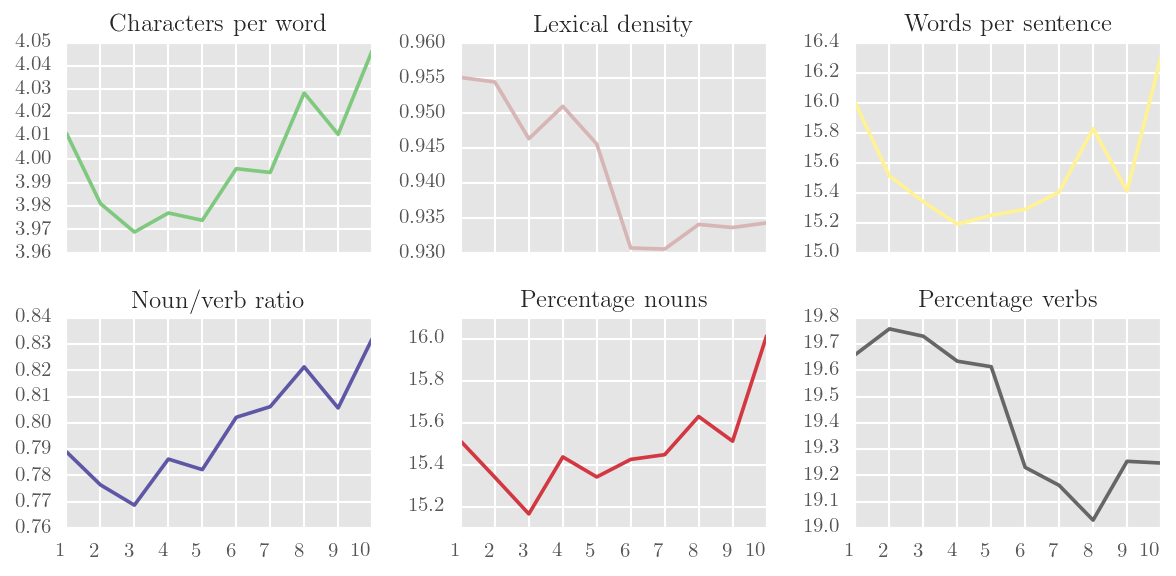
\includegraphics[width=\textwidth]{../images/derived-shallow-features-in-p-corpus.png}
\caption{Derived shallow features for the Membership Stage Structure}
\label{fig:derived_shallow_P}
\end{figure}

A number of features exhibit relatively consistent longitudinal change (see Figure \ref{fig:derived_shallow_P}). Many of these features point toward an increasingly `scientised' register \cite{harvey_disclosures_2012}, such as nominalisation and word length, which are related, as nominalisation typically involves the addition of derivational morphemes to non\hyp{}nominals \cite{simon-vandenbergen_grammatical_2003}. In the same vein, verbs become less frequent over time. That said, \emph{noun} and \emph{verb} are formal categories that can only approximate semantic notions of \emph{Things} and \emph{Events}, or, at a higher rank, \emph{Participants} and \emph{Processes}. More attention will be paid to these in the chapters that follow.

%\begin{figure}[htb]
%\centering
%\includegraphics[width=0.7\textwidth]{../images/firstpost-example.png}
%\caption{A first post example, featuring a medical history narrative}
%\label{fig:firstpost-example}
%\end{figure}

Another trend visible in Figure \ref{fig:derived_shallow_P} is that the first subcorpus---that is, first \glspl{post} to the \gls{Forum}---has features that often differ from the overall upward or downward trend. Lexical density (defined here as the ratio of lexical words to clauses) is one example: peaking in first \glspl{post}, it remains relatively stable thereafter. First \glspl{post} also deviate from general trends in terms of average character per word, words per sentence, noun\slash verb ratio, and the relative frequency of nouns in general. These features indicate that first \glspl{post} are considerably more packed with content than later contributions. Higher lexical density in first \glspl{post} is to be expected: \glslink{member}{users} are under no time constraints, as they are not responding to an interlocutor, and because other \glspl{member} are not aware that a message is being prepared. At the same time, users' initial contributions are more formal because it is in these contributions that new \glspl{member} first make interpersonal demands (solicitation of responses) on other \glspl{member}, who are by definition more senior figures in the community. Many \glslink{member}{users} may also have longer\hyp{}term considerations in mind: their first \glspl{post} constitute an initial bid for acceptance by the \glslink{Forum}{community}, and thus are tailored to conform to others' expectations of politeness. After the user is welcomed into the \glslink{Forum}{community}, lexical density quickly stabilises, and many other features begin a stable trajectory. These are early quantitative indications of a difference between the first and non-first \glspl{post} at the strata of \emph{genre} and \emph{register}. This discussion will be picked up in Chapter \ref{chap:discuss-bp}, following the presentation of findings from more delicate querying of the \GLS{lexicogrammar} in Chapters \ref{chap:interpersonal} and \ref{chap:experiential}.

\section{Controlling for self-selection bias}

The Membership Stage Structure has the potential for self-selection bias: \glslink{member}{users} who become veterans may use language differently even in their first \glslink{post}{contributions}. To control for this, the Future Veteran Structure (which contains no \glspl{post} from early dropouts) and the Comparative Structure (which has subcorpora for Dropouts and Future Veterans) can be used. In the section below, I briefly demonstrate that the language use of those \glslink{member}{users} who progress to veteran stages is not quantitatively different from the language of \glslink{member}{users} who drop out during early \glslink{post}{contributions}. The implication of this finding is that future veteran members' language choices do in fact change in predictable ways over time.

% I perform a limited number of investigations of these two \glspl{corpus}, in order to

\subsection{Future Veteran Structure}

The Future Veteran Structure contains no \glspl{post} from \glspl{member} who dropped out before contributing 30 times. It is structured identically to the Membership Stage Structure. When using this \gls{corpus}, the first four stages of membership are collapsed into a single stage, in order to make sure that each subcorpus contains a quantifiably reliable amount of text.

%\begin{table}
%\centering
%\small
%\begin{tabular}{lrrrrrrr}
%\toprule
%{} &    Verb &    Noun &  Pronoun &  Preposition &  Adverb &  Determiner &  Adjective  \\
%\midrule
%01 &   13491 &   10387 &     8236 &         6432 &    5126 &        4297 &       4229  \\
%02 &   20555 &   16320 &    12919 &         9834 &    7989 &        6679 &       6347  \\
%03 &   36500 &   28904 &    23048 &        17425 &   14048 &       11805 &      11328  \\
%04 &   71660 &   56816 &    45953 &        34037 &   27859 &       23313 &      21867  \\
%05 &  134443 &  105099 &    86145 &        63164 &   51718 &       43531 &      40638  \\
%06 &  178530 &  143212 &   114036 &        84616 &   69463 &       59305 &      55074  \\
%07 &  172483 &  139058 &   110574 &        81344 &   67335 &       57616 &      53652  \\
%08 &  185094 &  152034 &   117622 &        90276 &   72004 &       62675 &      59043  \\
%09 &  161888 &  130437 &   102969 &        78575 &   62341 &       55102 &      49909  \\
%10 &  156886 &  130532 &    99547 &        81309 &   56942 &       55112 &      48051  \\
%\bottomrule
%\end{tabular}
%\caption{Word classes in V Corpus}
%\label{tab:wc_V}
%\end{table}

\begin{figure}[htb]
\centering
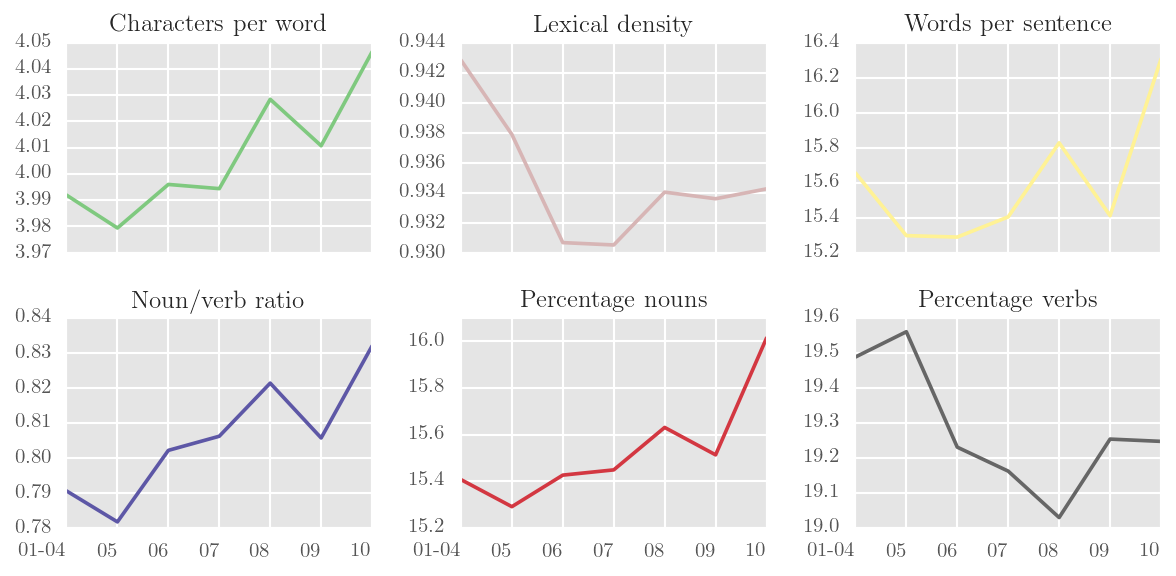
\includegraphics[width=\textwidth]{../images/derived-shallow-features-in-v-corpus.png}
\caption{Derived shallow features for the Future Veteran Structure}
\label{fig:derived_shallow_V}
\end{figure}

There is generally little difference from the Membership Stage Structure (compare with Figure \ref{fig:derived_shallow_P}), suggesting that future veteran \glslink{member}{users} use a similar register to non\hyp{}future \glspl{member} in early \glspl{post}.

\subsection{Comparative Structure}

Comparative Structure has two subcorpora: the first contains \glspl{post} from any \gls{member} who \glslink{post}{posted} fewer than 30 times; the second contains the \glspl{post} of members who \glslink{post}{posted} 30 or more times.

\begin{figure}[htb]
\centering
\includegraphics[width=0.6\textwidth]{../images/derived-shallow-features-in-C-corpus.png}
\caption{Derived shallow features for the Comparative Structure}
\label{fig:derived_shallow_C}
\end{figure}

Figure \ref{fig:derived_shallow_C} shows a great deal of similarity between the \glspl{post} of Dropouts and the early \glspl{post} of future Veterans. This means that broad register features change over the course of membership.

\section{Mapping membership stages to Forum history}

The Longitudinal Structure takes \glspl{thread} as the unit of analysis, rather than \glspl{post}. Each \gls{thread} is grouped by the year in which it was created, so that language change across the \gls{Forum}'s history can be examined. This corpus contains speaker metadata, making it possible to track one or more specific speakers longitudinally.

\begin{figure}[htb]
\centering
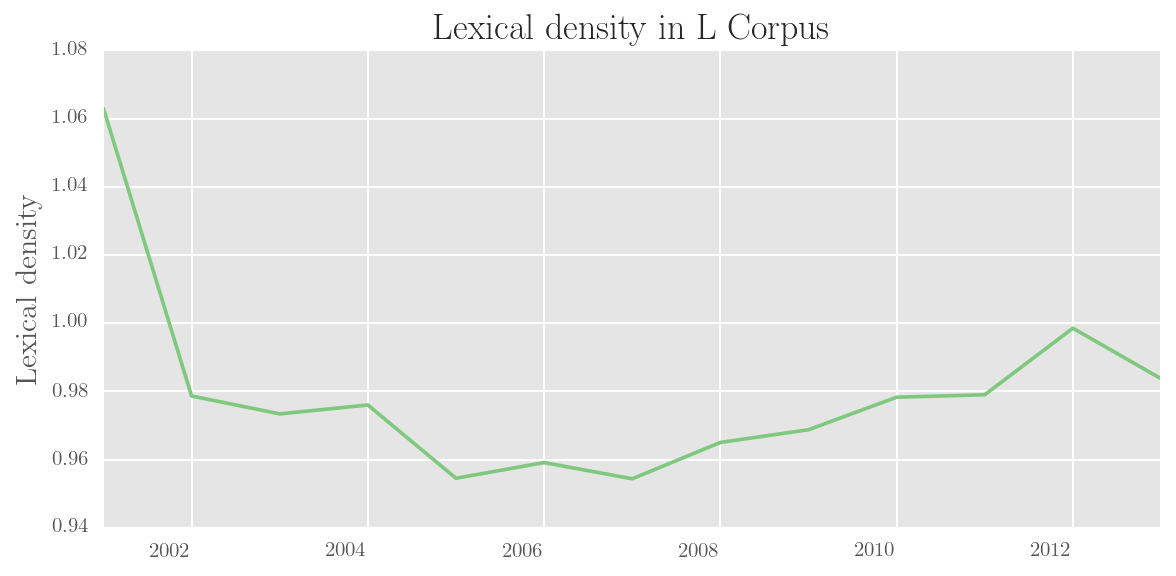
\includegraphics[width=0.6\textwidth]{../images/lexical-density-in-l-corpus.png}
\caption{Lexical density in the Longitudinal Structure}
\label{fig:lex_dens_L}
\end{figure}

%todo: this passage and the one below repeat point about generational change ...
Figure \ref{fig:lex_dens_L} shows that the Longitudinal Structure does not vary consistently in most shallow feature dimensions. One exception is in lexical density, which steadily rises throughout much of the \gls{Forum}'s history---fluctuations observed in the first and last subcorpora could well be the result of chance (due to their smaller sample size---see Section \ref{sect:l-corpus}). That said, it is not impossible that the first ever contributions to a \gls{forum} adopt a slightly more formal tone, as users air on the side of (polite) caution until the normative linguistic practices of the community take shape. The finding also hints at phylogenesis change, where linguistic practices of one generation of users within the \gls{Forum} can have a lasting effect on the practices of the next \cite{danescu-niculescu-mizil_no_2013}.

Though limitations of scope prevent a larger analysis of the Longitudinal Structure, it provides preliminary support for the notion that veteran \glslink{member}{users} may have lasting change on the discursive orientation of an online community. In terms of methodology, it demonstrates the utility of dynamic subcorpus structures: the same data, differently organised, can be analysed with identical methods in order to answer a different set of research questions. The Longitudinal Structure allows observation of the relationship between language use and the passage of time. Given our knowledge that ideologies are embraced and abandoned within the community at different points in time, it is reasonable to hypothesise that the time at which a new user enters the community could have an effect on the values they represent in later stages of membership. 

\section{Chapter summary}

In this chapter, I have provided preliminary analysis of the Bipolar Forum Corpus from two opposite perspectives. First, I have approached three \glspl{post} within a single \gls{thread} from below, looking at realised words and wordings in sequence. This analysis highlighted differences in how Forum members use language over the course of membership, in many respects finding existing discourse-oriented \gls{OSG} literature: newcomers' first \glspl{post} may conform to a first\hyp{}\gls{post} genre in which medical histories and current problems are outlined, with the dual aim of both legitimating the self as a potential member and eliciting responses from readers.

Second, I have looked at the corpus from above, looking at broad changes in shallow grammatical features, without consideration of the role of lexis, or of the distinction between metafunctions. Findings here showed that some features vary in more or less consistent ways over the membership course, and may be related to overall shifts in the register of users as they progress toward veteran status within the community. What remains, however, is to fill in the middle ground between realised samples of text and broad grammatical features. This analysis, segmented by metafunction into \sctext{Mood} and \sctext{Transitivity} parts, is performed over the next two chapters.

%!TEX root = ../thesis.tex

\chapter{MOOD and MODALITY choices in the Forum} \label{chap:interpersonal}

With an overview of shallow linguistic features in each \gls{corpus}, as well as a basic qualitative understanding of \glspl{post} and their generic properties, the investigation can begin to shift toward individual grammatical systems and the lexical choices at the most delicate end of each system's instantiative cline.

In this chapter, I present findings from an analysis of \sctext{Mood} and \sctext{Modality} choices, which are responsible for making interpersonal meanings---that is, they are used to negotiate the roles and responsibilities of interactants. Frequencies for choices of Mood and Indicative Type are calculated first. This is followed by an account of modalisation, Mood Elements, and brief descriptions of \sctext{tense} and \sctext{polarity} systems.%
\endnote{M\scriptsize{OOD}\footnotesize~structure is not well\hyp{}annotated in most typed dependency grammars currently used for parsing. As such, M\scriptsize{OOD}\footnotesize~features need to be derived from verbose constituency queries. A possible reason for this is that most parsing tasks are experientially or textually oriented. Furthermore, parsers are typically trained on \glspl{corpus} containing very few non\hyp{}declarative clauses.}

%todo: flag methdological opening?
\section{Mood and Indicative Type}

% this figure is contained here because it messes up
% syntax highlighting for the rest of whatever file
% it's in. the reason is that the highlighter doesn't
% understand that we're switching between tex, python
% and regexes.

\begin{figure}[htb]
\centering
\begin{minted}[linenos,breaklines,frame=single,xleftmargin=1cm,breakindent=0em,breaksymbolindentleft=0em]{python}
# salutations and exclamations that cause parser errors
badwords = ['-l.b-', 'hi', 'hey', 'hello', 'oh', 'wow',
            'thankyou', 'thanks', 'welcome',  'thank']

# mood types as dict object
m = {'Mod. declarative':
       r'ROOT < (S < (/(NP|SBAR|VP)/ $+ (VP < MD)))',
     'Unmod. declarative':
       r'ROOT < (S < (/(NP|SBAR|VP)/ $+ (VP !< MD)))',
     'Interrogative':
       r'ROOT << (/\?/ !< __)',
     'Imperative':
       r'ROOT < (/(S|SBAR)/ < (VP !< VBD !< VBG !$ NP !$ SBAR < NP !$-- S !$-- VP !$ VP)) !<< (/\?/ !< __) !<<- /-R.B-/ !<<, /%s/' % as_regex(badwords)}
\end{minted}
\caption{Tregex queries for Major clause Mood Types}
\label{fig:mood_dict}
\end{figure}

\begin{figure}[htb]
\centering
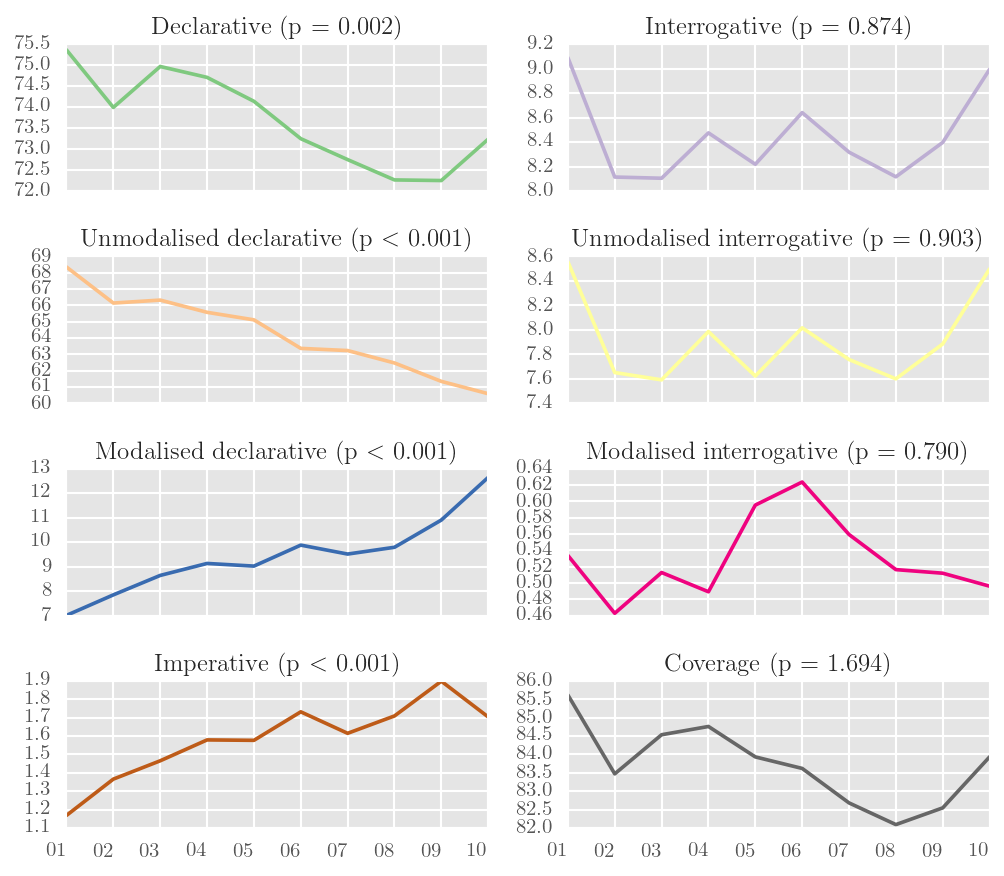
\includegraphics[width=0.8\textwidth]{../images/known-mood-and-indicative-types-in-p-corpus.png}
\caption{Mood features in the Membership Stage Structure}
\label{fig:mood_types_P}
\end{figure}

The broadest features of the \sctext{Mood} system that is reliably annotated by constituency parsing are the distinctions between Indicative and Mood Type (see Section \ref{sect:sfl}). Because dedicated tags for Mood Types are not available in either the constituency or dependency grammars, however, accurately locating them by automated searching alone is an unintuitive task. For this case study, \texttt{Tregex} expressions were developed, in order to discern major Mood and Indicative features from constituency parse trees (see Figure \ref{fig:mood_dict}). These queries must not just be designed for ideal, well\hyp{}formed cases, but must also handle false positives, such as sentence initial vocatives and salutations, which are often parsed as subject NPs. For interrogative matching, after many attempts to exploit Wh\hyp{}pronouns, Subject\hyp{}Finite order, it was determined that counting sentence final tokens containing at least one question mark was the most accurate method. When developing the constituency queries, accuracy was preferred over coverage. For this reason, only main clauses were analysed. To test the coverage of the queries, the total number of Mood Types found was compared to the total number of sentences (i.e. parse trees), minus any tree that did not contain a VP headed by a verb found in \texttt{VerbNet}. This removed a number of common, non\hyp{}major clausal parse trees, such as those provided for a minor clause like \emph{Hello!}.
%ntodo: verbnet reference?

\begin{table}
\centering
\footnotesize
\begin{tabular}{lrrrrr}
\toprule
{} &  Mod. declarative &  Unmod. declarative &  Interrogative &  Imperative &  Coverage \\
\midrule
$01$ &             $7.012$ &              $68.350$ &          $9.521$ &       $1.168$ &    $86.051$ \\
$02$ &             $7.849$ &              $66.143$ &          $8.618$ &       $1.366$ &    $83.976$ \\
$03$ &             $8.643$ &              $66.324$ &          $8.527$ &       $1.466$ &    $84.959$ \\
$04$ &             $9.132$ &              $65.576$ &          $8.967$ &       $1.579$ &    $85.254$ \\
$05$ &             $9.023$ &              $65.115$ &          $8.777$ &       $1.577$ &    $84.492$ \\
$06$ &             $9.880$ &              $63.367$ &          $9.183$ &       $1.732$ &    $84.163$ \\
$07$ &             $9.515$ &              $63.234$ &          $8.780$ &       $1.615$ &    $83.144$ \\
$08$ &             $9.792$ &              $62.474$ &          $8.640$ &       $1.710$ &    $82.616$ \\
$09$ &            $10.904$ &              $61.347$ &          $8.853$ &       $1.899$ &    $83.003$ \\
$10$ &            $12.645$ &              $60.592$ &          $9.283$ &       $1.704$ &    $84.224$ \\
\bottomrule
\end{tabular}
\caption{Relative frequency of Mood types}
\label{tab:mood_types_p}
\end{table}

The frequency of imperatives rises steadily through membership length (see Table \ref{tab:mood_types_p} and Figure \ref{fig:mood_types_P}), as veteran \glspl{member} may explicitly direct new \glspl{member} to do certain things: \emph{take care}, \emph{find the right meds}, or \emph{watch alcohol consumption}, for example, are common commands issued in veterans' \glspl{post}. Though advice given through imperatives provides suggested behaviour (as in the cases above), heavy grammatical constraints on the imperative mood (lack of Subject, tense, etc.) make elaboration within this kind of advice uncommon. Modality is also difficult to encode, as modal Finites cannot grammatically modify imperative Predicators (\emph{*Could go to the doctor}!). Imperatives thus rarely carry information regarding the addressee's level of obligation or the speaker's level of certainty or source of knowledge, and accordingly, can be face\hyp{}threatening for newcomers \cite{goldsmith2004communicating,hudson1990discourse}. For this reason, in veterans' \glspl{post}, unmodulated imperatives often function as general markers of social support (\emph{take care of yourself}; \emph{keep up the good work!}) rather than as suggested behaviour coupled with health information or marking of the source of the knowledge. Thus, there is no one-to-one relationship between the extent to which \gls{Forum} users make interactive demands on others and choices of Mood Type.

As shown in Table \ref{tab:mood_types_p}, declaratives shift over time, from unmodalised toward modalised type. This indicates a correlation between membership stage and the extent to which \glslink{member}{users} insert judgements of likelihood of propositions. This pattern can be interpreted as evidence of increasing social status over time. At the same time, however, the \sctext{Modality} system can be used as a resource for signalling incongruence between Speech Function and Mood Type (see the following section). Interrogatives, on the other hand, undergo no significant trajectory shift, as demonstrated in the significance calculations shown in Figure \ref{fig:mood_types_P}. Questions therefore comprise the same amount of talk at all stages of membership. As will be discussed below, while the overall frequency of the interrogative Mood remains stable, the kinds of propositions being negotiated in these questions undergo observable longitudinal change.

The calculation of \emph{Coverage} (Table \ref{tab:mood_types_p}\slash Figure \ref{fig:mood_types_P}) shows that the proportion of sentences for which Mood Type information could be obtained fluctuated, but in no clear direction. This increases confidence that observed changes in Mood Type proportions are not the result of consistent language changes that cause an increase or decrease in parser accuracy.

\section{Modalisation} \label{sect:modalisation}

Modalisation construes uncertainty within the clause as exchange. It is a more delicate feature of the \sctext{Mood} system than Mood Type, because its meaning changes depending on Mood selection: in declaratives, it congruently involves a speaker judgement; in interrogatives, it demands judgement from the addressee \cite{halliday_introduction_2004}. Different modal lemmata are responsible for communicating obligation, certainty, probability and usuality; at the same time, choices in modal lexis distinguish between low, median and high uncertainty, with negative and positive polarity at either pole (see Section \ref{sect:mood-grammar}: \sctext{Modality}).

%\begin{figure}[htb]
%\centering
%\includegraphics[width=0.6\textwidth]{../images/modals-when-subject-is-emphi.png}
%\caption{Mood features for the Membership Stage Structure}
%\label{fig:modalsb}
%\end{figure}
%
Over the course of membership, in general, Modalisation as a feature of Major clauses increases consistently (from 6.67\% to 8.83\% of all clauses). The major Mood Type accommodating this increase is the modalised declarative (Figure \ref{fig:mood_types_P}). A primary cause of this change is a strategy for advice provision that develops over the membership course. Rather than simply issuing commands with imperatives, much advice dispensed by veterans is realised by declaratives, generally featuring modalisation (see Figure \ref{fig:imp_and_mod} for examples). 

% modal examples
\begin{figure}
    %\minipage{0.44\textwidth}\centering
    \begin{tabular}[t]{@{}>{\raggedright\arraybackslash}p{0.45\textwidth}}
    \vspace{1mm}
    %\noindent\parbox[t]{0.44\textwidth}{\raggedright%
    \begin{enumerate} [before=\itshape,font=\normalfont] \setlength\itemsep{0em} \footnotesize
    %\item Keep talking and being patient ... it will happen but it isn't going to happen overnight like we all would like it too.
    \item Let us know how your appointments go!!
    \item Keep us posted with how things go.
    \item Keep on posting and let us know how you are doing.
    %\item Tell her what you just told us here... that you are not sleeping and that you knew that the wellbutrin was making you feel good with the mania but that you are afraid.
    %\item Make that call, Llama... you need to before this gets too out of hand and you are unable to know the difference.
    %\item Ask her if there is anything that you can do to make her feel better.
    %\item Get up and walk if you are able to for short periods of time... take your meds when you need to and a week after you feel better to cover things well.
    \item Try to pretend that you have a suit of armor on and try to allow as much of this to bounce off of you.
    \item Get a good night's sleep, eat right eliminating caffeine \& sugar from your diet, take your meds as prescribed, avoid stress as much as possible, get plenty of exercise and hold onto your sense of humor.
    \end{enumerate}
    \end{tabular}
    \begin{tabular}[t]{@{}>{\raggedright\arraybackslash}p{0.45\textwidth}@{}}
    
    \begin{enumerate}  [before=\itshape,font=\normalfont] \singlespacing \setlength\itemsep{0em} \footnotesize
    \item I would certainly make a point to follow up
    \item I would definitely have your daughter pay her
    \item I would highly recommend it
    \item I would DEFINITELY recommend seeing a psychologist
    \item I would definitely make mention of this
    \item I would strongly suggest that you discuss
    \item I would be very careful with just the Zoloft
    \item I would highly recommend that you take your meds on a daily basis.
    %\item I would also suggest you call NAMI.
    \end{enumerate}
    \end{tabular}
    %\endminipage
    \caption{Advice provision via imperatives and modalised declaratives}
    \label{fig:imp_and_mod}
    \end{figure}
    %
    \begin{figure}[htb]
    \centering
    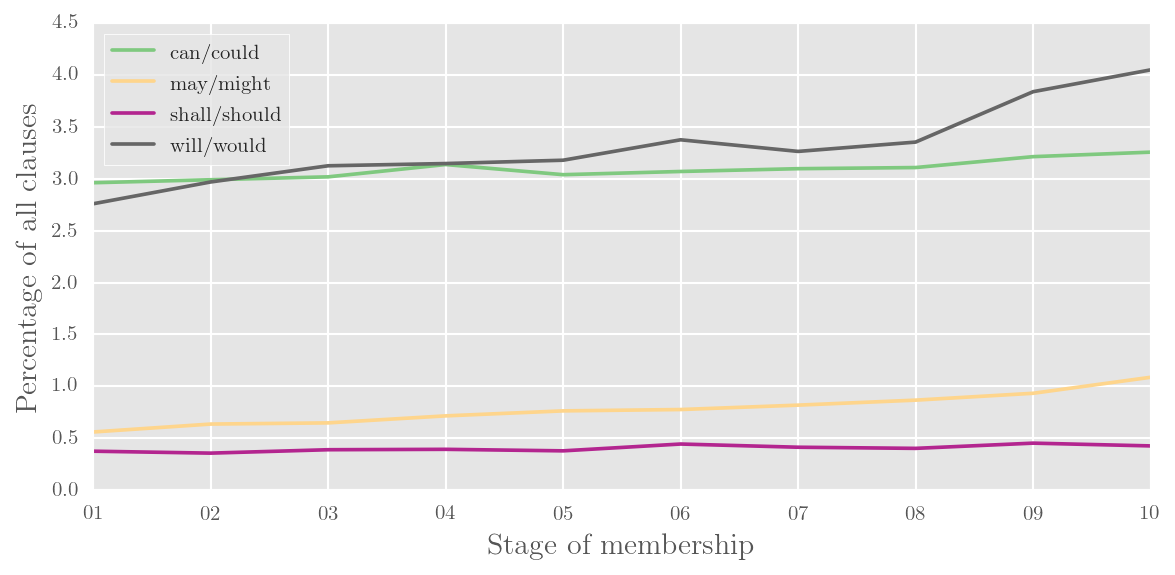
\includegraphics[width=0.6\textwidth]{../images/modalnew.png}
    \caption{Relative frequencies of modal lemmata}
    \label{fig:modals}
    \end{figure}
%
Figure \ref{fig:modals} shows that over the length of membership, there is a particularly marked increase in the frequency of \emph{would\slash will} modals, in comparison to other modal lemmata. Concordancing of declaratives modalised by \emph{would} was performed in order to understand their typical contexts of use. This revealed three things. First, veterans commonly dispense advice through hypothetical \emph{I would} statements (as in the examples above, and as seen in the qualitative analysis of Emz' post in Section \ref{sect:qual-reply-analysis}). Second, the modalised declarative is also often modulated by an Adjunct, in order to reconstitute perlocutionary force that was diminished through the incongruent selection of Mood Type (\emph{I would seriously\slash really\slash certainly consider quitting}). Third, the same grammatical construction also exists in new \gls{member} talk, but very rarely as a means of giving advice. Rather, \emph{I would (+ adjunct}) in first \glspl{post} often introduces a construal of past behaviour (\emph{I would get seriously drunk every night}---see Figure \ref{fig:vetmember_would} for contextualised examples).

%todo: split methods and findings a bit better?
As a result of this ambiguity, all \emph{I $+$ would $+$ adjunct} declaratives in new and veteran \glspl{member}' \glspl{post} (261\slash 143 total matches) were coded according to five inductively developed functional categories (outlined in Table \ref{tab:themcodes}). Three false positives (where \emph{'d} as a contraction of \emph{had} had been incorrectly parsed as a contracted \emph{would} modal) were excluded from analysis. The categories are not codified in the \gls{SFG}; rather, they are based on the apparent meaning potential of the register of \gls{Forum} talk. Categories are also not intended to be discrete: since a core purpose of modalisation is to express inclination, most instances of \emph{I would + adjunct} are on some level statements of inclination. Not all statements of inclination are descriptions of past behaviour, or provisions of advice, however.

%\emph{Will}-modalisation is also increasingly common over membership length. Issues of scope prevent its treatment here.}~

% 'jess' provides a future will modal in the qual analysis
   
% i would functions
\begin{table}[htb]
    \centering
    \footnotesize
    \begin{tabularx}{\textwidth}{p{2cm}XX}
    
    \toprule
    Category    & Description & Example       \\ \midrule
    Past Behaviour       & Habitual (generally negative) actions in the past   & \emph{And was around the time I would occassionally go to sleep for as much as 24 hours}     \\ 
    Advice       & Suggesting what another should do & \emph{I'd really encourage you to just call your psychologist back}    \\ 
    Request     & Requesting actions (typically information\slash support provision) from others      & \emph{I'd really appreciate any feedback from anyone on here}          \\
    Inclination and hypothetical & Preferences and inclinations, often in irrealis scenarios (within if-clauses) & \emph{I would never want to be without him; I wish I were sicker so that I wouldn't even worry about it} \\ 
    Hedged salutation            & Self introduction, explicit salutation      & \emph{I'm new here so I thought I'd just start out with a big ol' hi} \\ 
    Past sense of \emph{will}           & Talk of the future within narratives about the past---usually in Verbiage     & \emph{My father always told me that I would never mount to anything}   \\ \bottomrule
    \end{tabularx}
    \caption{Thematic categories of \emph{I would} + adjunct}
    \label{tab:themcodes}
    \end{table}
                    
    \begin{figure}[htb]
    \centering
    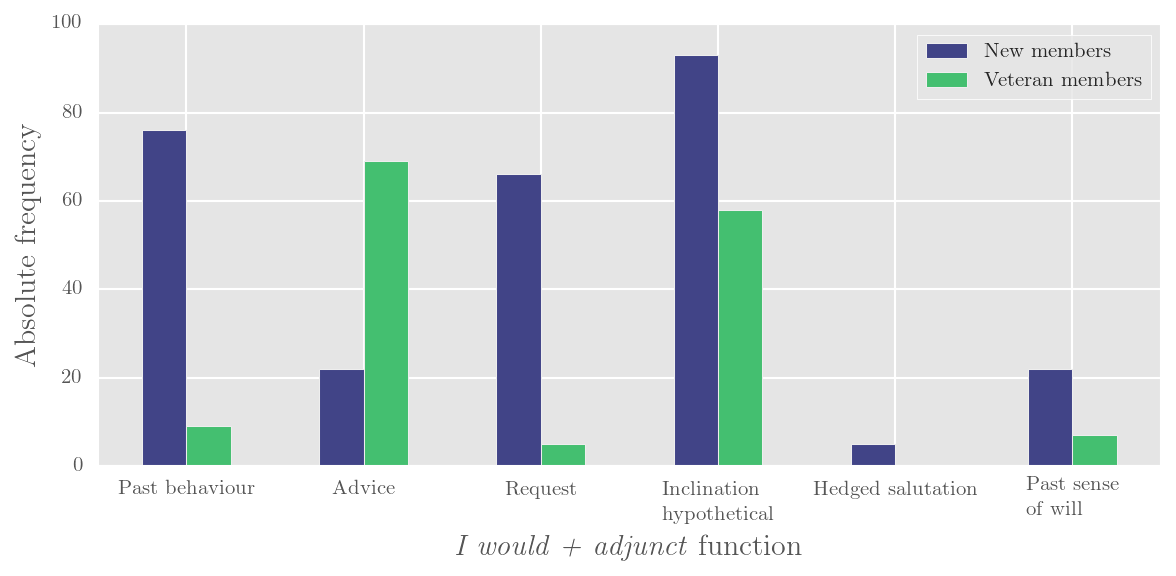
\includegraphics[width=0.75\textwidth]{../images/iwould-vid.png}
    \caption{Functions of \emph{`I would'} in new and veteran posts}
    \label{fig:i_would_func}
    \end{figure}
    
            %Concordancing \emph{would}-modalised declaratives in veteran posts revealed a distictive lexicogrammatical pattern for the provision of advice.
    
            %\enumsentence{\small{\emph{so many times i would walk over 40 km from my home to the city center, looking for people that didn't exist, at times i would even think beggars were spies ... or supernatural characters, very deluded and very weird ... many times i wouldn't sleep for at least 3 days, one time i didn't eat and sleep for 4 days !!!} (New member, post 1)}} % frokly
            %\enumsentence{\small{\emph{I would suggest that you go to the ER, explain your symptoms and then apply for assistance through a program like Medicaid} (Veteran member, post 1166)}} % dreamsinneon
    
                %\begin{figure}
                %  \centering
                %  \addvbuffer[12pt 8pt]{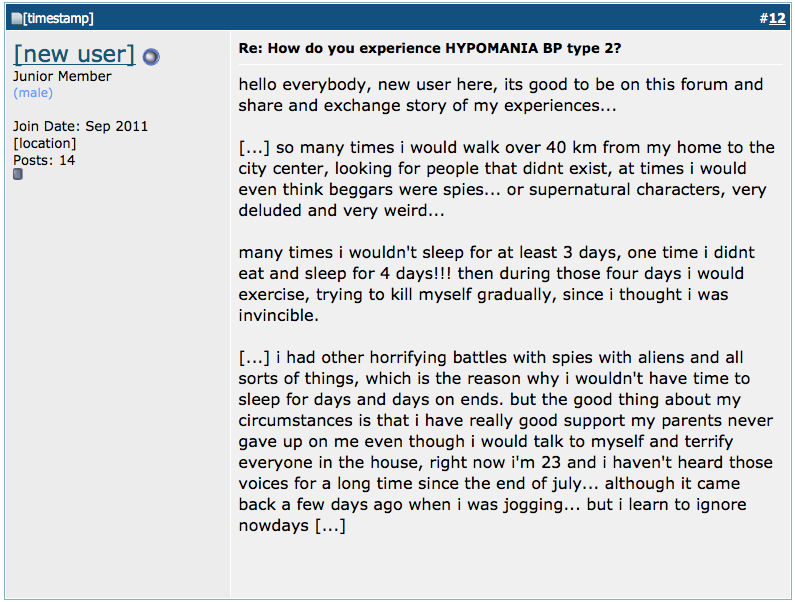
\includegraphics[width=0.65\textwidth]{../images/new_member_would.png}
                %  \caption{A new member's ``\emph{I would}'' construction}
                %               %\end{figure}
    
                %\begin{figure}
                %  \centering
                %  \addvbuffer[12pt 8pt]{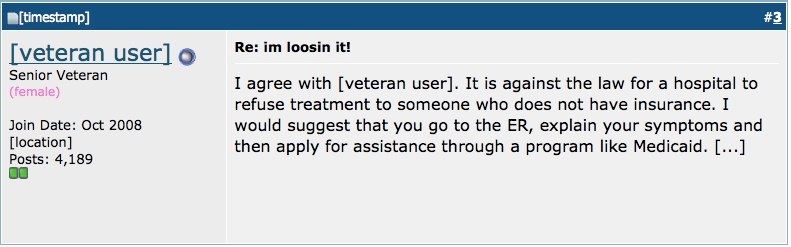
\includegraphics[width=0.65\textwidth]{../images/veteran_member_would.png}
                %  \caption{A veteran member's ``\emph{I would}'' construction}
                %  \label{fig:vetmember_would}
                %\end{figure}
    
Figure \ref{fig:i_would_func} shows that new and veteran members employ the \emph{I would + adjunct} construction for different purposes. In newcomer talk, it is commonly used to make incongruently realised requests (\emph{I would like to know ...}). This is a politeness strategy---veteran members seldom hedge their requests in this way. Also more common in newcomer talk are the uses of \emph{I would + adjunct} to index \emph{Past behaviour}, and as the \emph{Past sense of will}, an example of which can be found in Jess's first \gls{post} (\emph{i want to change my doctor and have been telling my partner i would}---see Section \ref{sect:jess-post}). From the perspective of genre, as highlighted in the previous Chapter, initial contributions conforming to generic structures include a substantial medical history, told in the past tense. For veterans, on the other hand, \emph{I would + adjunct} is predominantly used to signal advice. Aside from the general category of \emph{Inclination and hypothetical}, other functions are very uncommon in \glspl{post} made during the final stage of membership.

% The fact that manual analysis is necessary for such specific work highlights shortcomings in available \gls{NLP} tools. As such, when counting features, we must bear in mind that they may perform multiple functions. Chapter \ref{chap:futuredirections} discusses needed steps to automate this kind of categorisation.

%todo: is there a reference for this?
Advice realised by an \emph{I would} reveals much about the ways in which role relationships within the \glslink{Forum}{community} are discursively constructed. In contrast to health professionals' advice, \emph{I would} puts the veteran hypothetically in the position of the newcomer, highlighting their shared role as people living with \gls{bipolar}. At the same time, however, it stakes claim to higher social status: the construction implies not just a burden on the addressee to follow the advice, but also some more subtle social values---that veterans know more, and that the course of action they would personally take in such a situation is the right one. 

An experiential analysis of the \emph{I would} style of advice provision complements the interpersonal perspective here. The advice giver is construing him\slash herself experientially as the main participant in the figure, substituting the newcomer out of the construed reality entirely. This main participant is almost always an Agentive one: the most common processes include \emph{suggesting}, \emph{talking}, and \emph{going}. To emphasise agency further, veteran \glspl{member} may embed advice within a material process of \emph{going} (see Table \ref{tab:conc_iwould_action}), especially when the addressee is to be the Medium in the presented figure (\emph{I would go and get evaluated ...}). In turn, this emphasis on agency highlights for the addressee the need to take action in order to gain control over his\slash her health problems.

% conc: i would go and get ...
\begin{table}[htb]
\footnotesize
\begin{tabular}{rrl}

\toprule
        i wouldn't just &  go         &  and quit ... perhaps it is time to look for a less stressful job \\
                                        i'd &  go         &  right away and ask for major help from your pdoc \\
i would most definitely &  go         &  and be evaluated by a psychiatrist, that is absolutely the only way  \\
             n your shoes i would &  go         &  and get a second opinion from a doctor you've not been to before.              \\
                                     i would &  go         &  and get evaluated for bipolar if you thing that is what you have \\
and then i would &  go         &  talk with the pdoc and ask him why these meds .                                  \\
                      but i would definitely &  go         &  for that eval.                                                                  \\
\bottomrule
\end{tabular}
\caption{Emphasising action in veterans' advice to newcomers}
\label{tab:conc_iwould_action}
\end{table}
%
This foregrounding of subjective knowledge is very much at odds with Harvey's \citeyear{harvey_disclosures_2012} finding, where adolescents used a medicalised register to legitimate their claims. In the \glslink{Forum}{Bipolar Forum}, legitimacy is claimed explicitly through lay experience. While newcomers typically enter the \glslink{Forum}{community} with specific requests for information (about a side\hyp{}effect of a medication, or a problem with insurance, for example), veterans demonstrate an understanding of the illness course as a whole, with advice often taking into account a `bigger picture' that the newcomer is assumed to be not yet privy to. 

% examples of i would as html
\begin{figure}[htb]
\minipage{0.48\textwidth}\centering
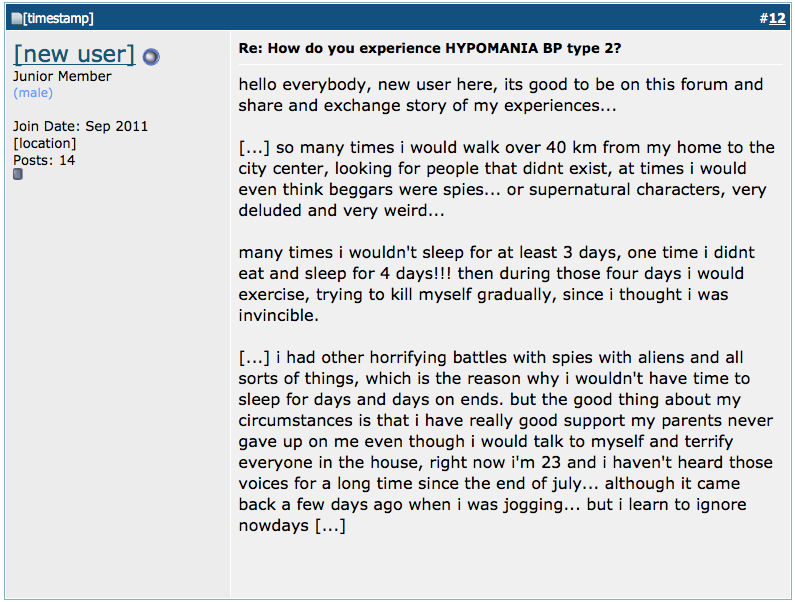
\includegraphics[width=1.00\textwidth]{../images/new_member_would.png}
\endminipage\hfill
\minipage{0.48\textwidth}\centering
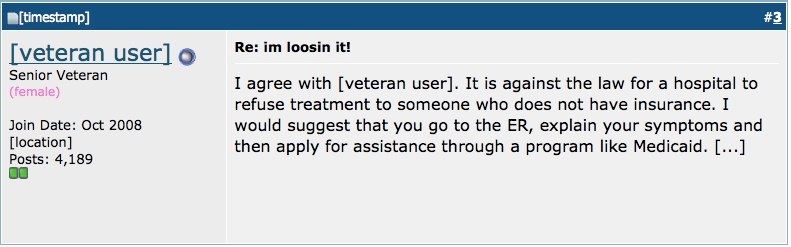
\includegraphics[width=1.00\textwidth]{../images/veteran_member_would.png}

\raggedright
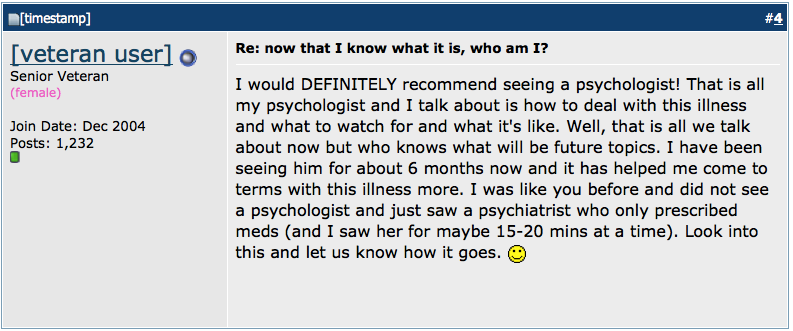
\includegraphics[width=1.01\textwidth]{../images/vet2would.png}

\endminipage\hfill
\caption[New and veteran members' `\emph{I would}' constructions]{Examples of typical new and veteran members' `\emph{I would}' constructions}
\label{fig:vetmember_would}
\end{figure}

%As the \glslink{Forum}{community} has a strong biomedical orientation, however, in which only health professionals can perform felicitous diagnosis, veteran members limit their advice to management through lifestyle choices, rather than medication regimens or new diagnoses.

%must mark their advice as grounded in lay-expertise. The issuance of imperative commands is a less common strategy than the use of incongruent modalised declarative commands. To reconstitute the force of the command, without overstepping the line that divides lay and professional kinds of health knowledge, veteran members employ adjuncts.

%The veteran's lay experiences---especially those experiences that occurred between his/her experience as a newcomer and the present moment---are construed as sufficient 

\FloatBarrier
\section{Mood elements}

In \gls{SFL}, the Finite grounds a proposition in time and space, making it \emph{arguable}. Arguability can be centred on primary tense, where propositions are debated with respect to when they occurred, in relation to the time of speaking. Alternatively, Modality can be argued. The Subject, meanwhile, is the thing charged with ensuring the carrying out of the proposition. By interrogating the \gls{corpus} for combinations of Subjects and Finites \cite[see][]{eggins_introduction_2004}, it is possible to chart change in who is made responsible, in the clause\hyp{}as\hyp{}exchange.

% Pronoun-Subject + Modal-Finite blocks as a percentage of all clauses in the P Corpus
\begin{figure}
    \centering
    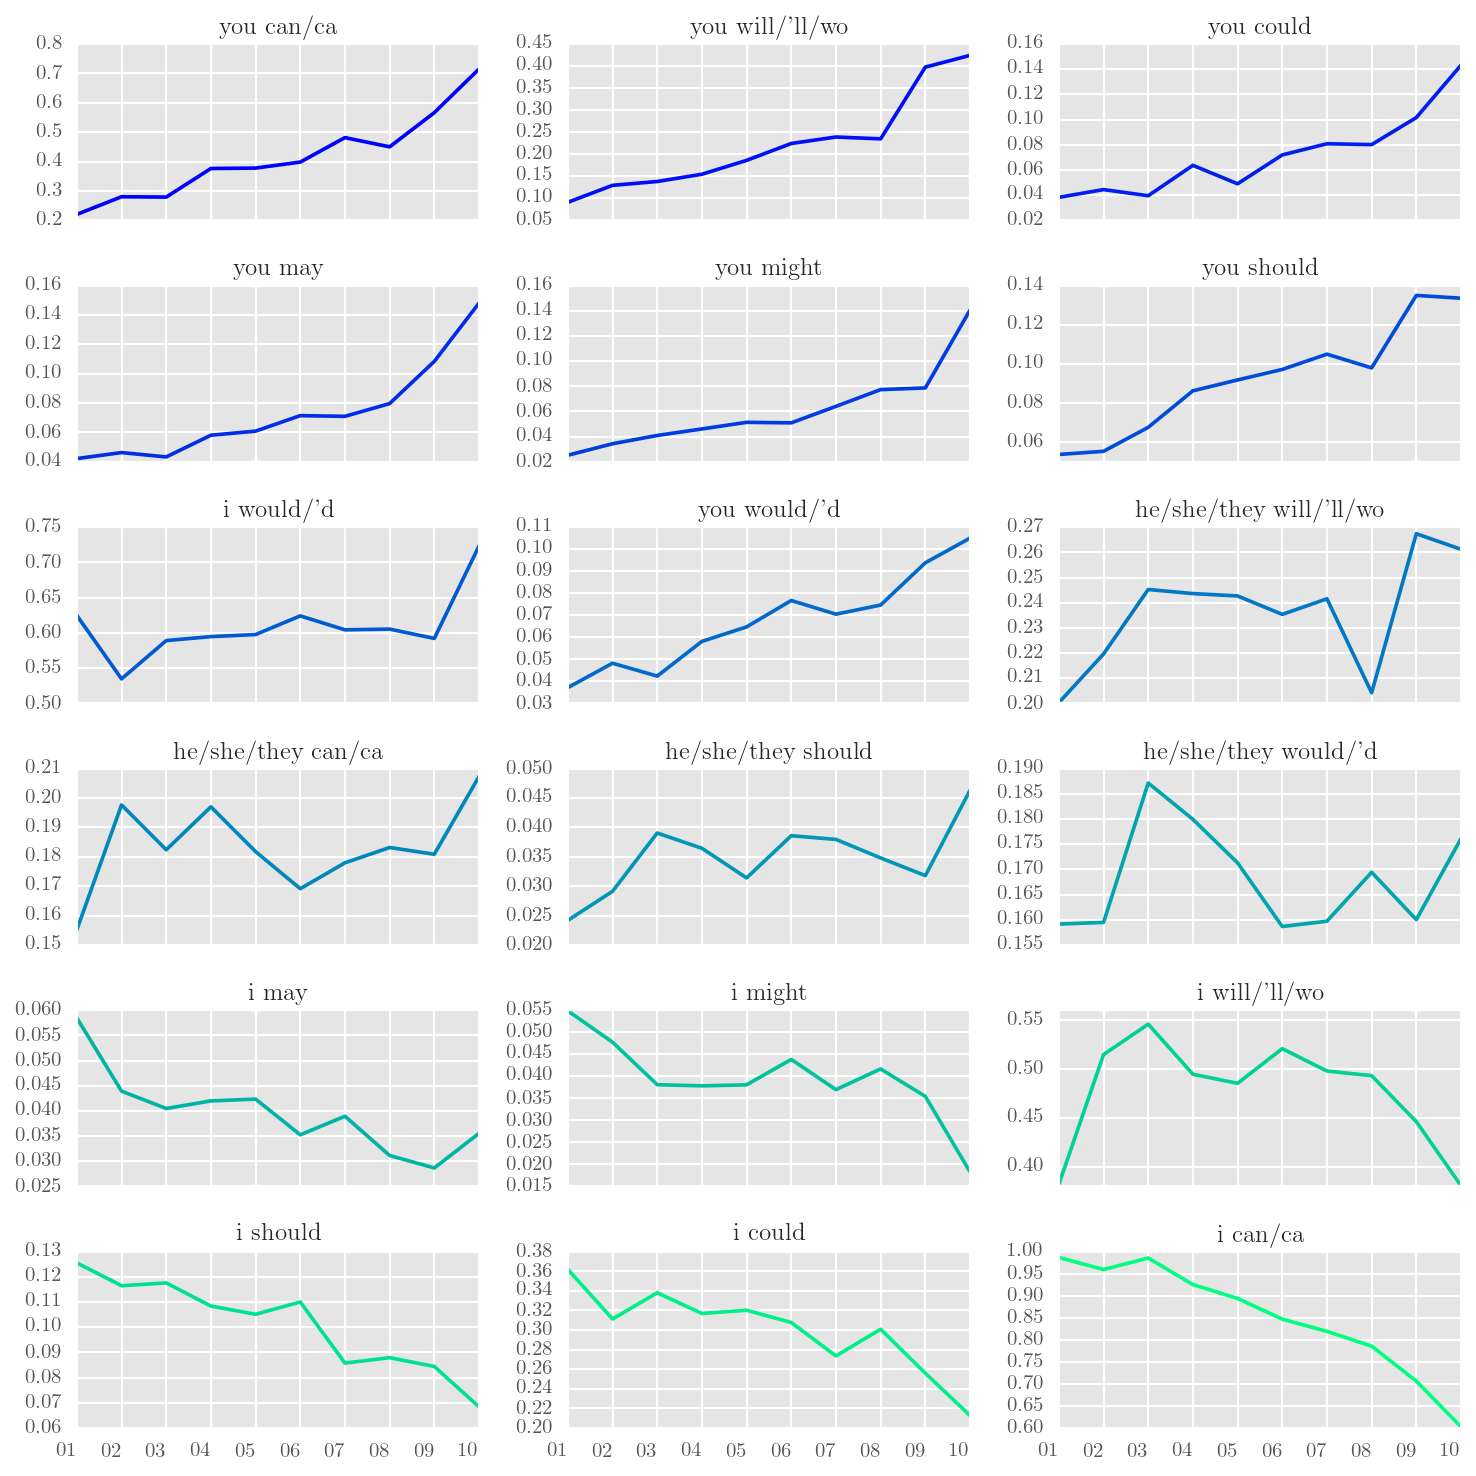
\includegraphics[width=1\textwidth]{../images/subj-fin-const-p-page.png}
    \caption[Pronoun-Subject + Modal-Finite blocks]{Pronoun-Subject + Modal-Finite blocks as a percentage of all clauses}
    \label{fig:modal_constellations}
    \end{figure}%
%
The frequencies and trajectories of configurations of Pronominal subjects and modal Finites can be used to determine the kinds of proposals and propositions being debated. Figure \ref{fig:modal_constellations} shows that generally, \emph{I $+$ modal} is displaced by \emph{you $+$ modal} over the course of membership. In fact, \emph{I would} stands out as the only \emph{first person $+$ modal} block on an increasing trajectory. This is due to its frequent use as a means of giving advice, as discussed above. Though modals negotiate a diverse range of concepts, such as certainty, probability and obligation, the \emph{Subject $+$ modal} configuration still places an interpersonal burden on the Subject as the one charged with bringing the Predicator about. Accordingly, newcomers self\hyp{}assign the burden, while veteran members turn to direct interpersonal demands on their interlocutors. This is not to say, of course, that the veteran\slash newcomer relationship is one that mistreats the newcomer. The dynamic is a symbiotic one. Veteran membership comes with a kind of expertise, which is being exchanged with other \glslink{Forum}{community} members through advice. Veterans answer others by explaining what is possible, feasible, likely or uncertain.

Mood Blocks can also be viewed through the lens of \glslink{Forum}{community} membership conditions. In early \glspl{post}, \glslink{member}{users} narrate their medical history, setting out credentials for acceptance by the user base. Veteran \glspl{member} act as interviewers, requesting further information, or grafting the presented narratives to the community's normative biomedical ideology. Newcomers are under observation, and are expected to assist in veterans' assessments by providing a narrative account of their illness course. This is particularly important in first \glspl{post}, but extends generally to cover early contributions, in which the new user is primarily focussed on the self.

Figure \ref{fig:modal_constellations} also shows that the trajectory of \emph{third person $+$ modal} constructions is generally inconsistent or stable. This is because role\hyp{}relationship negotiation is carried out by making or fulfilling the demands of interlocutors, rather than things and people being spoken about. There is therefore little difference over the course of membership in the way non\hyp{}present participants are modalised. Rather, as we will see later, non\hyp{}present participants undergo a number of changes within the system of \sctext{Transitivity}.

Of all constellations, \emph{I $+$ can} (and its derivatives and interrogative inversion) undergoes the most radical change. In a question, this kind of Mood Block expressly asks others for information or permission. As can be seen in Table \ref{tab:conc_i_can_first}, in first \glspl{post}, in declarative form, \emph{I can} is very often negated, with contributors narrating difficulties carrying out healthy mental processes (\emph{cope, focus, make up mind, handle\slash stand it, stand it, remember own name, have no emotion, feel normal}), controlling harmful behavioural processes (\emph{can't stop crying, can barely stay awake, can't breathe}), and performing vague material processes (\emph{get things done, nothing I can do about it, get out of everyday life}). Over the membership course, the construction falls into disuse: unlike \emph{I would}, it is very rarely employed as a proposal (e.g. \emph{I can PM you this if you like}).

% Concordancing \emph{I can} mood blocks in first \glspl{post}
\begin{table}[htb]
    \footnotesize
    \begin{tabular}{lrl}
    \toprule
    0  &  antly stressed , i had migranes and &  i could n't sleep , i could n't go out for to long be\\
    1  &  ad migranes and i could n't sleep , &  i could n't go out for to long because i just always \\
    2  &  s just started to get abit better , &  i could go out again                                 \\
    3  &  nd i did want to end it all because &  i could n't take the fear anymore                    \\
    4  &              i ' v also noticed that &  i can get really angry , really easily these days too\\
    5  &   - if anyone has any tips about how &  i can lose weight and not gain anymore whilst on depa\\
    6  &  st but i 've coped with it the best &  i can                                                \\
    7  &     i~'m not working right now , but &  i ca n't seem to get anything done around my house   \\
    8  &  t have tutors come to my house when &  i could handle them                                  \\
    9  &  f out of bed in the morning and all &  i can think about all day                            \\
    10 &                                      &  i can not stop crying .                              \\
    11 &                                      &  i can barely stay awake .                            \\
    12 &   i feel so fat and disgusting , but &  i ca n't stop eating                                 \\
    13 &                          i just wish &  i could make them feel how i 'm feeling , just so the\\
    14 &  al and i feel like there 's nothing &  i can do about it                                    \\
    15 &  erally just keep thinking about how &  i can go back to the psych ward                      \\
    16 &  go back to the psych ward , just so &  i can get out of everyday life for a while           \\
    17 &                                      &  i can not get along with any of my coworkers , as wel\\
    18 &                                      &  i ca n't process any of my rapid thoughts and have ju\\
    19 &                                      &  i ca n't think of any reason why this occurs and do n\\
    \bottomrule
    \end{tabular}
    \caption[Concordancing \emph{I $+$ can} Mood Blocks]{Concordancing \emph{I $+$ can} Mood Blocks in first \glspl{post}}
    \label{tab:conc_i_can_first}
    \end{table}
%
This pattern can also be approached in terms of membership entry conditions. Newcomers often stress the seriousness or urgency of their case, based on the existence of some ongoing mental or physical harm.

\subsection{Tense}
%todo: the two figures presented here get reversed due to size, which i don't like

\FloatBarrier

If not by \sctext{Modality}, arguability happens along the lines of \sctext{Tense}---the relationship between a proposition and the time of speaking. Figure \ref{fig:tense_constellations} shows different configurations of pronominal Subject and Tense. More specifically, it shows that tense of modals is not a feature that exhibits consistent change over time: the trajectory shifts are caused for the most part by changing frequencies of pronominal Subject choice.

% Tense of tensed clauses over the course of membership
\begin{figure}[htb]
\centering
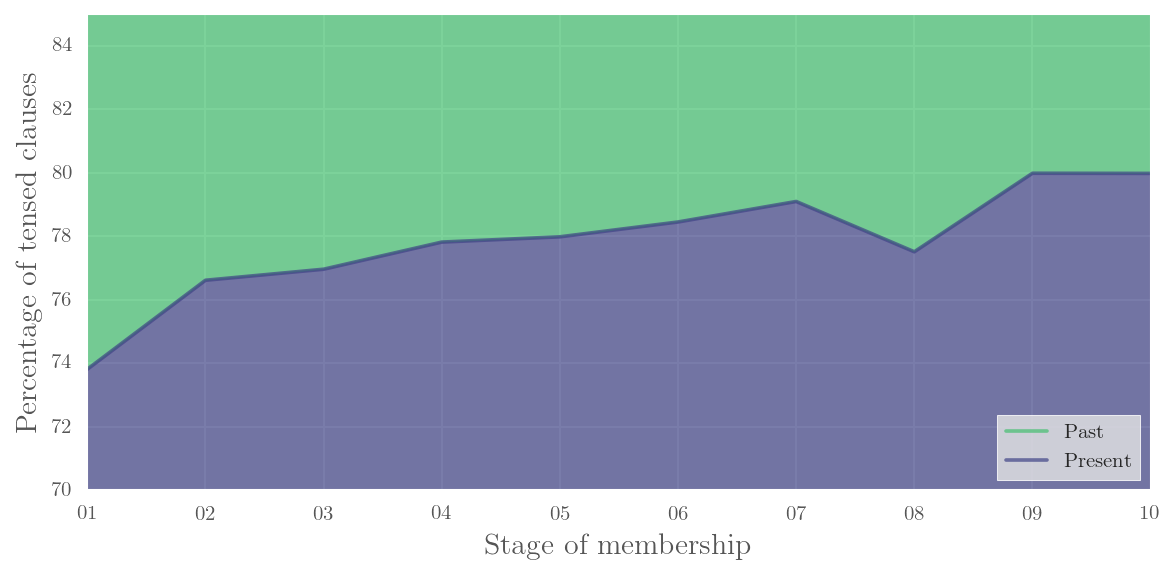
\includegraphics[width=.7\textwidth]{../images/tense-area.png}
\caption{Tense of tensed clauses over the course of membership}
\label{fig:tense-area}
\end{figure}
%
The system of \sctext{Tense} can be isolated from its co\hyp{}text, however. Figure \ref{fig:tense-area} plots primary tenses of non\hyp{}modalised clauses over the membership course. The steady transition from past toward present (from 74 to 80 per cent of all tensed clauses) demonstrates a shifting focus from setting out medical history narratives as membership credentials to helping others with their current problems. At an ideological level, the shift also represents a gradual refocussing on present and future actions, both of the self and of addressees.

% Pronoun-Subject + Past\slash Present tense blocks as a percentage of all Major clauses in the P Corpus
\begin{figure}[htb]
\centering
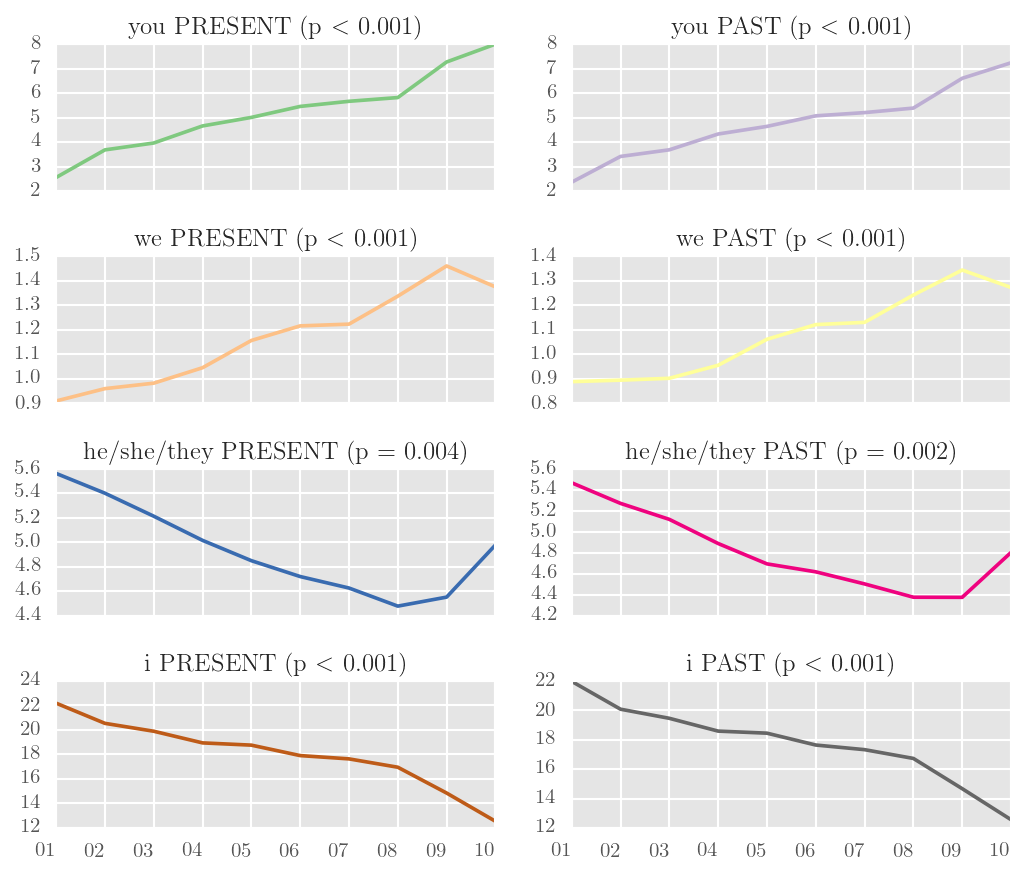
\includegraphics[width=1\textwidth]{../images/subj-ten-const-p.png}
\caption[Pronoun-Subject + Past\slash Present tense blocks]{Pronoun-Subject + Past\slash Present tense blocks as a percentage of all Major clauses for the Membership Stage Structure}
\label{fig:tense_constellations}
\end{figure}

\subsection{Polarity}

The final component of the interpersonal analysis is the system of \sctext{Polarity}.\endnote{There was little reason to expect dramatic or consistent polarity shifts over the course of membership. The analysis is carried out and presented mostly for the purposes of completeness of the register description.}~Clauses may have positive or negative polarity. The default polarity is positive; negative polarity is realised through a small group of lexical items (\emph{n't\slash not}, \emph{no}, \emph{never}) that appear in close proximity, or fused with, the Finite. Therefore, polarity can be interrogated using \texttt{Tregex} queries:

\begin{verbatim}
Negative = 'VP !> VP <+(VP) (VP !< VP <<# (/VB.?/ < /$VERBLIST/)) \
           ' <<# /(VB.?|MD)/ < (RB < /(?i)^(n.t|never|no)$/)'
Positive = 'VP !> VP <+(VP) (VP !< VP <<# (/VB.?/ < /$VERBLIST/)) \
           ' <<# /(VB.?|MD)/ !< (RB < /(?i)^(n.t|never|no)$/)'
\end{verbatim}

\begin{figure}[htb]
    \centering
    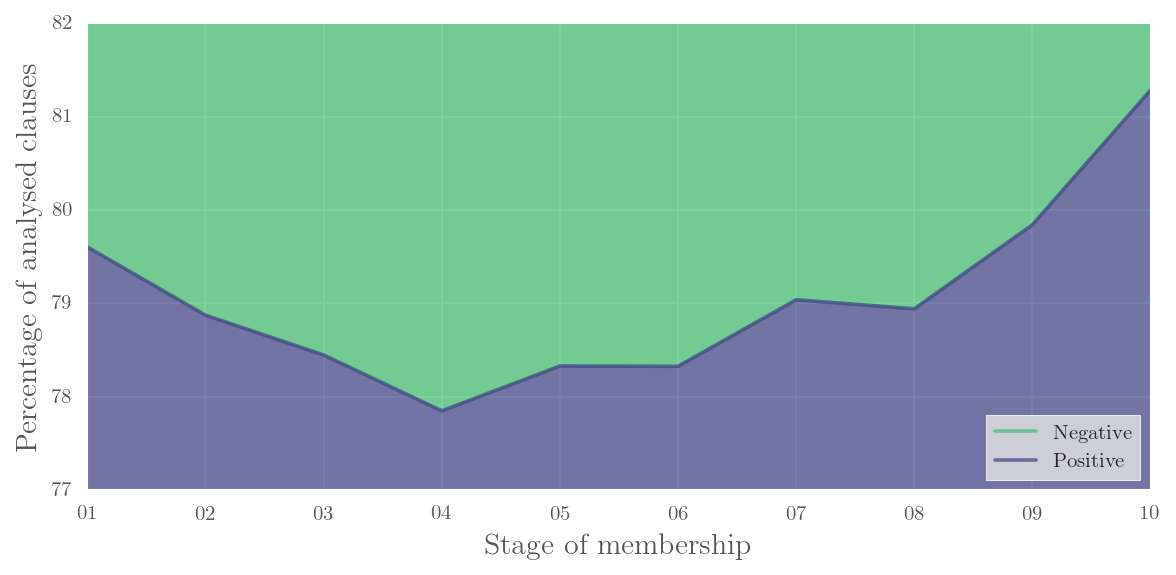
\includegraphics[width=.7\textwidth]{../images/polarity-area.png}
    \caption{Clause polarity over the course of membership}
    \label{fig:polarity}
    \end{figure}

\sctext{Polarity} figures into other places within interactions, such as as minimal responses to polar interrogatives. These kinds of minor clauses are not considered here; only clauses containing a verb\hyp{}form in \texttt{WordNet} are considered. Figure \ref{fig:polarity} shows that clause\hyp{}level polarity choices have an unstable trajectory over the membership course, decreasing until the 8--15th post, and then increasing. The fact that this result is difficult to interpret is unsurprising: the meaning of polarity is to some extent dependent on Mood Type, and on the previous move in the exchange. Moreover, unlike a linguistic feature like passivisation or grammatical metaphor, the ratio of positive\slash negative polarity clauses does not have a direct or clear relationship with \glspl{discourse-semantic} within a clause, except perhaps in a few rare cases (i.e. a list of rules). As noted in Section \ref{sect:mood-grammar}, \sctext{Polarity} is more likely to provide insights into discourse when examining entire interactions, rather than individual \glspl{post}. Even so, one point of note is that negative polarity is approximately twice as frequent as the ratio (ten per cent of all clauses) suggested by \textcite{halliday_introduction_2004}.

It is also possible to search for polarity in combination with other Mood features, in order to determine whether combinations of Modality $+$ Polarity, or Pronominal Subject $+$ Polarity, are undergoing change. In Figure \ref{fig:subjmodpol}, modals are grouped into four types. Distinctions are also made between first and second person Subjects, and between positive and negative polarity. Again, this kind of analysis shows, when compared to choices of Subject and modal, polarity choices play only a minor role in the longitudinal register shift of \glspl{member} of the \glslink{Forum}{Bipolar Forum}.

% subj mod pol
\begin{figure}[htb]
    \centering
    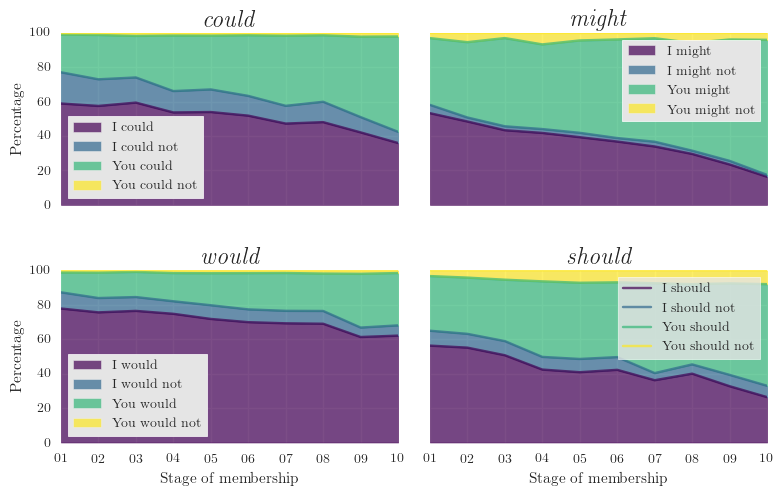
\includegraphics[width=.8\textwidth]{../images/subjmodpol.png}
    \caption{Constellations of Subject, Modal and Polarity}
    \label{fig:subjmodpol}
    \end{figure}
% analysis

\section{Summary}

Mood and Indicative Types shift across the course of membership: imperatives and modalised declaratives become more frequent as users gain the social capital necessary to dispense advice or make (semiotic) demands on newcomers. Interrogatives do not exhibit a clear trajectory, because the \glslink{Forum}{community} roles of both veterans and newcomers involve asking questions. For newcomers, questions are a means of obtaining information from the longer\hyp{}term users; for veterans, questions are used to elicit information that may aid in advice provision. Questions can be used to demonstrate interest and investment in the narratives of others, and to hold others accountable for perceived absences from the group (\emph{Where did ya go?}); alternatively, they can be used to invite newcomers to return to the community and\slash or to contribute again \cite{paulus_`please_2015}.

%todo copy edit
\sctext{Modality} is used throughout membership, with increases in later stages. Exploration of \emph{I $+$ would} clauses reveals shifts in the socio\hyp{}semantic activities in which \gls{Forum} members engage, from narration of past circumstances (\emph{sharing}) toward hypotheticals and suggestions for further behaviour \cite[\emph{advising}---see][]{matthiessen_applying_2013,matthiessen_modeling_2015}. This, however, is a registerial insight that blends components of Field and Tenor \cite{Matthiessen2015}. Looking at Mood Blocks more generally, a clear transition takes place over the course of membership: new and veteran members alike co\hyp{}operate to hold the less senior \glspl{member} modally responsible in discourse. The system of \sctext{Tense} exhibits change when modal tense is excluded, showing a longitudinal orientation toward the present and future, away from the past. \sctext{Polarity} is shown to vary inconsistently when analysing \glspl{post} alone, and to generally play a subordinate role to other components in the \sctext{Mood} system.

In the next chapter, I use dependency parses to investigate longitudinal changes in experiential meanings made in the \gls{Forum}, via choices of \sctext{Transitivity}.

%!TEX root = ../thesis.tex

\chapter{TRANSITIVITY choices in the Forum} \label{chap:experiential}

In Chapter \ref{chap:interpersonal}, I analysed \sctext{Mood} and \sctext{Modality} features of the \gls{corpus}, discussing findings with respect to interpersonal meaning\hyp{}making in the \glslink{Forum}{community}. This chapter uses similar methods to focus on experiential meanings, and their realisation within \sctext{Transitivity} choices. This allows observation of how inner (mental) and outer (physical) states are represented by \gls{Forum} \glspl{member}. \sctext{Transitivity} analysis of a clause involves distinguishing between Process Types or ergativity (represented in the main verbal group), as well as participants (the arguments of the verbal group) and circumstances (which modify the meaning made by the process). In this chapter, the analysis of participants is performed first, and processes second. That said, more delicate queries often involve consideration of both, as well as their attendant modifiers and circumstances. Rather than using constituency grammar, this part of the investigation relies on dependency annotations, which more closely model the \sctext{Transitivity} system \cite{costetchi_method_2013}. Collapsed, conjunction\hyp{}processed dependencies are used in almost almost all cases \cite[see][]{manning_stanford_2014}.

For both participants and processes, the workflow is similar. Heads of groups are extracted from the \gls{corpus} and transformed into relative frequencies and keyword tables. Linear\hyp{}regression based sorting is used to determine which results are on increasing, decreasing, static and turbulent trajectories, in terms of both relative frequency and keyness. A subset of results undergoing obvious trajectory shifts are then analysed in greater detail, by probing their lexicogrammatical behaviour, and by concordancing. Profiles for these results, and for concepts indexed by sets of related lexis, are constructed in order to highlight differences in the way they are deployed in the subcorpora of each \gls{corpus} under investigation.

Because of the strong methodological focus of the thesis, results are typically presented without manual removal of parsing errors, or of phenomena that are vague or difficult to interpret. Where necessary, the cause of errors is discussed before moving forward to analysis of the generated result. The argument being advanced, both here and in later chapters, is that doing discourse analysis or \gls{CL}\slash \gls{CADS} can be automated to a greater extent than it thus far has been: targeted searches of the \gls{lexicogrammar}, exclusion of instances based on non\hyp{}arbitrary information, and trajectory\hyp{}based sorting can leave the analyst with summarised lexicogrammatical information with relatively obvious links to \glspl{discourse-semantic}. Unedited result lists are therefore presented in order to demonstrate both the promise of partially automated \gls{CL} methods and the seriousness of limitations in the method that are discussed in Chapters \ref{chap:discuss-bp} and \ref{chap:implications}.

\section{Participants}

To locate participants, a \gls{corpus} can be searched for the lemma forms of dependency nodes of particular types, roughly corresponding to distinctions made within the \gls{SFG}. For participant, the corresponding labels are \emph{acomp}, \emph{agent}, \emph{appos}, \emph{csubj}, \emph{csubjpass}, \emph{dobj}, \emph{iobj}, \emph{nsubj}, \emph{nsubjpass} and \emph{xsubj}. There are some inconsistencies between the grammars that are difficult to resolve, however: as one example, the Universal Dependency grammar used by \texttt{Stanford CoreNLP} annotates the Range in a process\hyp{}range configuration (\emph{I took a shower}) with the same label as it does a Goal (\emph{I built a shower}). Even so, there is a great deal of overlap between the grammars, especially in the case of the general distinction between process and participant.

% Relative frequencies of common participant heads in each P subcorpus
    \begin{table}[htb]
    \centering
    \small
    \begin{tabular}{lrrrrrrrrrr}
    
    \toprule
    Subcorpus &     i &   it &   you &   he &  she &  that &  they &   we &  what &  this \\
    \midrule
    $01$ & $32.22$ & $6.31$ & $ 3.48$ & $4.44$ & $2.87$ &  $1.88$ &  $1.84$ & $1.29$ &  $1.61$ &  $1.32$ \\
    $02$ & $30.13$ & $7.10$ & $ 5.09$ & $4.12$ & $2.87$ &  $2.17$ &  $2.16$ & $1.39$ &  $1.63$ &  $1.14$ \\
    $03$ & $29.49$ & $7.40$ & $ 5.46$ & $4.36$ & $2.47$ &  $2.25$ &  $2.18$ & $1.47$ &  $1.73$ &  $1.12$ \\
    $04$ & $28.08$ & $7.49$ & $ 6.44$ & $4.11$ & $2.22$ &  $2.29$ &  $2.25$ & $1.59$ &  $1.68$ &  $1.12$ \\
    $05$ & $27.67$ & $7.62$ & $ 6.91$ & $3.80$ & $2.18$ &  $2.33$ &  $2.35$ & $1.77$ &  $1.77$ &  $1.15$ \\
    $06$ & $26.51$ & $7.54$ & $ 7.52$ & $3.41$ & $2.36$ &  $2.47$ &  $2.29$ & $1.92$ &  $1.71$ &  $1.10$ \\
    $07$ & $26.02$ & $7.69$ & $ 7.82$ & $3.59$ & $2.07$ &  $2.44$ &  $2.38$ & $1.96$ &  $1.66$ &  $1.08$ \\
    $08$ & $25.18$ & $7.76$ & $ 8.05$ & $3.34$ & $2.06$ &  $2.54$ &  $2.32$ & $2.11$ &  $1.70$ &  $1.05$ \\
    $09$ & $21.91$ & $7.79$ & $10.06$ & $3.26$ & $2.39$ &  $2.78$ &  $2.24$ & $2.37$ &  $1.73$ &  $1.05$ \\
    $10$ & $18.65$ & $7.50$ & $11.14$ & $2.96$ & $3.32$ &  $2.88$ &  $2.44$ & $2.30$ &  $1.66$ &  $1.19$ \\
    \bottomrule
    \end{tabular}
    \caption[Relative frequencies of common participant heads]{Relative frequencies of common participant heads at each stage of membership}
    \label{tab:rel_freq_part_stop}
    \end{table}
%
%todo: long sentence :)
Because closed\hyp{}class words have not at this point been excluded, the most common participant heads are generally pronominal (Table \ref{tab:rel_freq_part_stop}). Even so, the shift from first toward second person participants, and the relative stability in third person pronoun usage, are both observable, echoing findings from the investigation of \sctext{Mood} choices, where first and second person pronouns feature prominently as Subjects, and where the latter come to displace the former in veteran talk. Within the domain of interpersonal meaning, the increasing second person as Subject indicated a shift in which interactant is charged with interactive demands. Within the system of \sctext{Transitivity}, however, the shift in meaning is an experiential one: \emph{who is being spoken about} changes over the course of membership, from the self toward the addressee (Table \ref{tab:rel_freq_part_stop}). 

% Keyness of common participant heads in three stages of membership
    \begin{figure}[htb]
    \centering
    \small
    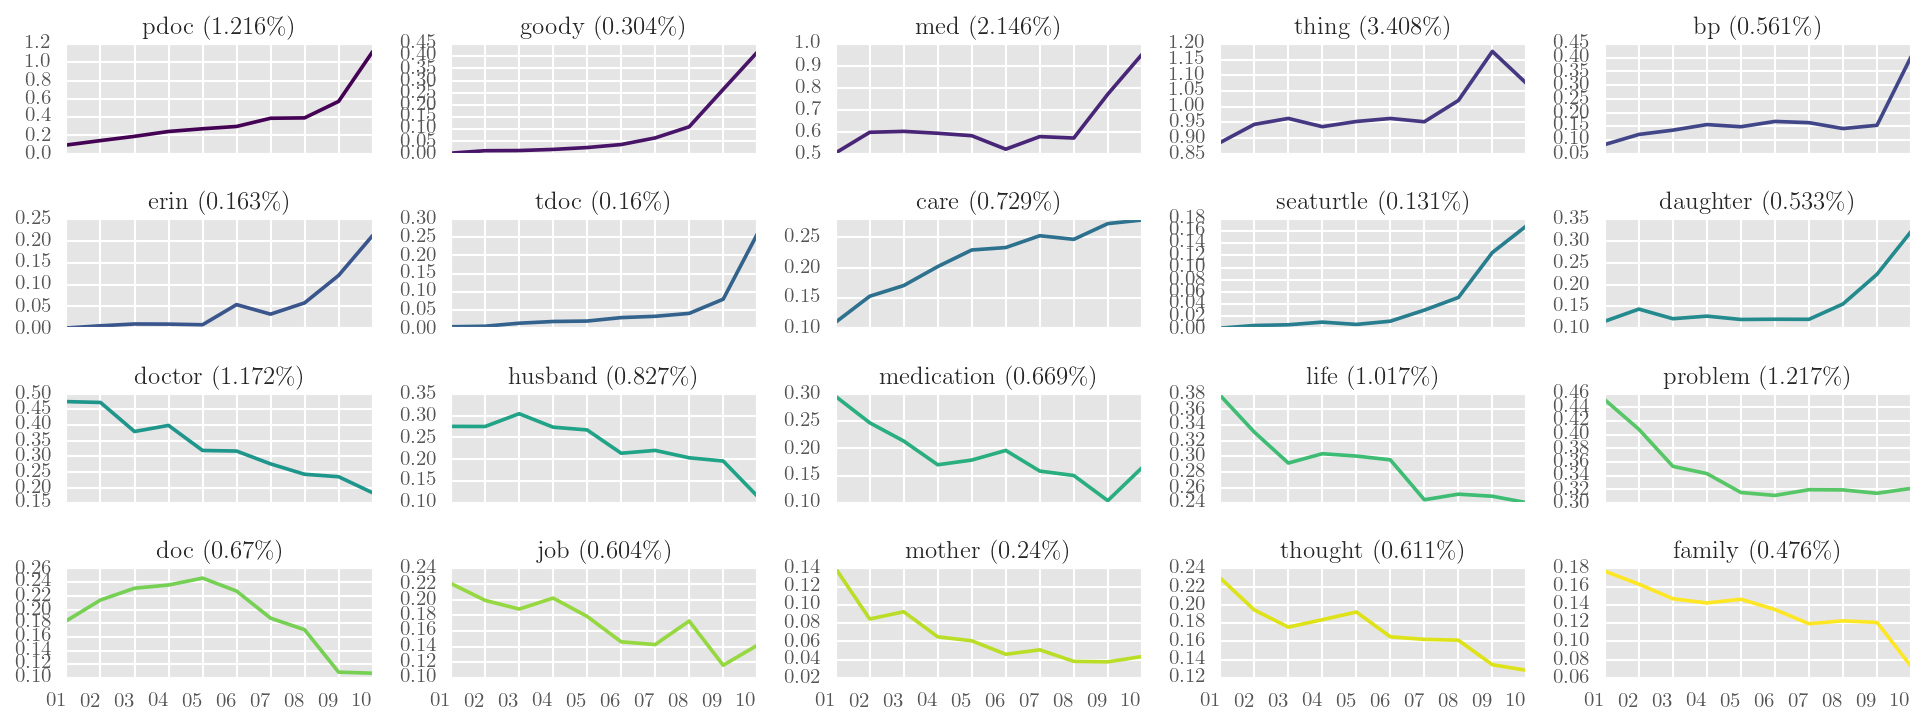
\includegraphics[width=1\textwidth]{../images/part-traj2.png}
    \caption{Trajectory of common participants undergoing change}
    \label{tab:key_part_w_prop}
    \end{figure}
%
Figure \ref{tab:key_part_w_prop} shows the longitudinal trajectories of common open\hyp{}class participant heads, as a percentage of all participants. From the 1000 most common heads, the ten on the most sharply increasing trajectory (top half), and the ten on the most decreasing (bottom half) are shown. Proper nouns denoting veteran \glspl{member} and their family\slash friends (\emph{seaturtle}, \emph{goody}, \emph{erin}, \emph{daughter}) dominate the `increasing' results because veteran \glspl{member} refer to one another and commonly discuss those close to them by name. Similarly, the declining frequency of \emph{husband} and \emph{mother} may have more to do with the particular circumstances of the small group of veteran members than it does to do with a normative value governing the ways in which the world ought to be construed by veteran members of the group. It is important to keep in mind, therefore, that the small sample of veteran \glslink{member}{users} can cause an over\slash under\hyp{}representation of particular participants. Fortunately, removing proper nouns is a trivial task, as they are annotated by \texttt{Stanford CoreNLP} with distinct \gls{POS} tags (\texttt{NNP}\slash \texttt{NNPS}). 

Table \ref{tab:keyunkey-threestage} shows the top participants, excluding pronominal and proper\hyp{}nominal words. It uses log\hyp{}likelihood keyness, rather than simple relative frequency, and collapses the ten subcorpora into three (\emph{Early stages}, \emph{Mid stages} and \emph{Late stages}). Discursive insights become clearer here---negative emotional lexis appears as key in early contributions, while more positive terms and jargon appear as key in later \glspl{post}. Before interpreting these, however, it is important to make note of the issue of parser accuracy, which has an impact on what is classified as a participant. \emph{Welcome} and \emph{thanks}, for example, are in some cases misannotated as participants. This is caused by short, minor clause sentences or sentence fragments, with which the parser model used is unfamiliar. Another problem is that some proper nouns have not been correctly removed: \emph{whiskey} and \emph{kait} are shorthand forms of two veterans' usernames, often misannotated as common nouns or adjectives. The misannotation is caused by the fact that the names may be written without capitalisation in the Forum---uncapitalised proper nouns, like minor clause sentences, are essentially absent in the parser training data.

%\begin{minted}[linenos,breaklines,frame=single,xleftmargin=1cm,breakindent=0em,breaksymbolindentleft=0em]{python}
%parts = corpus.interrogate(search={GF: roles.process,
%                                    F: roles.participant},
%                           exclude={W: wordlists.closedclass,
%                                    P: '^PRP'},
%                           show=[L])
%parts = parts.edit('k', SELF)
%\end{minted}
%

% key and unkey participants in collapsed stages of membership
\begin{table}[p]
    \centering
    \small
    \begin{tabular}{lrlrlr}
     \toprule
    Early stages &        & Mid stages &        & Late stages &         \\
    \midrule
          bipolar & $709.26$ &     person & $114.96$ &        pdoc & $2002.63$ \\
              new & $692.95$ &        doc & $ 97.41$ &        tdoc & $ 735.35$ \\
           doctor & $396.43$ &       hard & $ 87.91$ &         med & $ 339.99$ \\
       medication & $254.38$ &       luck & $ 73.50$ &        glad & $ 316.05$ \\
           mother & $229.52$ &         be & $ 66.70$ &         hug & $ 315.12$ \\
     psychiatrist & $178.40$ &       good & $ 61.09$ &   stability & $ 287.02$ \\
               dr & $161.91$ &        lol & $ 60.07$ &    daughter & $ 278.64$ \\
            swing & $159.18$ &    illness & $ 59.41$ &        able & $ 229.33$ \\
         medicine & $139.93$ &    whiskey & $ 55.67$ &         son & $ 208.47$ \\
          problem & $136.31$ &   kindness & $ 54.89$ &       thing & $ 193.58$ \\
            angry & $135.12$ &  happiness & $ 47.38$ &   important & $ 188.02$ \\
               mg & $125.84$ &         bp & $ 45.07$ &        okay & $ 176.41$ \\
           scared & $125.47$ &         dh & $ 39.75$ &     cycling & $ 170.74$ \\
          episode & $122.30$ &   positive & $ 39.68$ &  stabilizer & $ 162.11$ \\
              old & $121.93$ &      sorry & $ 35.97$ &       sorry & $ 128.38$ \\
             life & $120.06$ &        lot & $ 34.37$ &     welcome & $ 120.52$ \\
            crazy & $115.24$ &      peace & $ 33.37$ &        care & $ 120.31$ \\
          husband & $110.02$ &     spouse & $ 32.32$ &     support & $ 112.70$ \\
             kill & $109.40$ &     thanks & $ 30.39$ &        news & $ 111.06$ \\
       depression & $107.70$ &         ok & $ 29.78$ &      better & $ 101.82$ \\
             take & $104.63$ &      right & $ 29.18$ &       group & $  98.96$ \\
           normal & $100.55$ &       care & $ 28.60$ &        hear & $  93.55$ \\
             high & $ 99.87$ &      wendy & $ 28.49$ &   imbalance & $  93.49$ \\
            worse & $ 96.02$ &       time & $ 27.11$ &       treat & $  91.19$ \\
           attack & $ 93.26$ &      stuff & $ 26.96$ &  adjustment & $  90.46$ \\
    \midrule
     adjustment & $  -31.53$ &          sticky & $-25.49$ &     becuase & $ -35.54$ \\
         easier & $  -31.64$ &            kait & $-25.49$ &      normal & $ -37.82$ \\
           step & $  -33.05$ &      assessment & $-25.49$ &         cos & $ -38.51$ \\
           bper & $  -34.94$ &            earn & $-26.43$ &          nt & $ -39.22$ \\
           able & $  -36.00$ &       incorrect & $-26.43$ &       swing & $ -39.91$ \\
             bf & $  -36.68$ &             prn & $-26.43$ &       scare & $ -40.78$ \\
          right & $  -37.27$ &       marijuana & $-27.38$ &       moody & $ -41.95$ \\
         stable & $  -46.18$ &  hypersexuality & $-28.32$ &         god & $ -45.27$ \\
           okay & $  -48.81$ &             mil & $-28.32$ &         dad & $ -46.83$ \\
           post & $  -55.83$ &        disorder & $-28.80$ &       hyper & $ -46.92$ \\
             bp & $  -62.22$ &         cycling & $-28.88$ &    horrible & $ -48.12$ \\
         thread & $  -65.28$ &              ed & $-29.27$ &     bipolar & $ -48.65$ \\
           hear & $  -65.44$ &             son & $-29.57$ &  medication & $ -62.73$ \\
            tee & $  -67.39$ &       flashback & $-30.21$ &          dr & $ -65.39$ \\
      important & $  -78.59$ &    psychiatrist & $-30.60$ &       crazy & $ -66.38$ \\
           news & $  -80.07$ &         typeing & $-32.10$ &      thanks & $ -68.69$ \\
     stabilizer & $  -84.75$ &         titrate & $-32.10$ &      mother & $ -74.03$ \\
        welcome & $  -90.33$ &     impulsivity & $-32.10$ &      scared & $ -78.99$ \\
           care & $  -92.95$ &        daughter & $-34.83$ &         mad & $ -79.00$ \\
      stability & $ -103.53$ &            pdoc & $-34.99$ &     husband & $ -79.01$ \\
          sorry & $ -131.56$ &       stability & $-35.74$ &         doc & $ -84.92$ \\
            hug & $ -133.61$ &              hi & $-44.81$ &          mg & $-110.55$ \\
           glad & $ -210.66$ &         bipolar & $-86.69$ &    medicine & $-123.90$ \\
           tdoc & $ -309.27$ &             new & $-90.07$ &      doctor & $-196.93$ \\
           pdoc & $-1126.49$ &            tdoc & $-93.25$ &         new & $-241.95$ \\
    \bottomrule
    \end{tabular}
    \caption{Key and unkey participants in three stages of membership}
    \label{tab:keyunkey-threestage}
    \end{table}


A final view of overall participant frequencies is provided in Figure \ref{fig:key-traj}. This figure only charts trajectory changes among the 200 most frequent participants. This has the useful effect of automatically excluding many erroneous results.

% Relative frequencies of common participants in each P subcorpus, decreasing
\begin{figure}[htb]
    \centering
    \small
    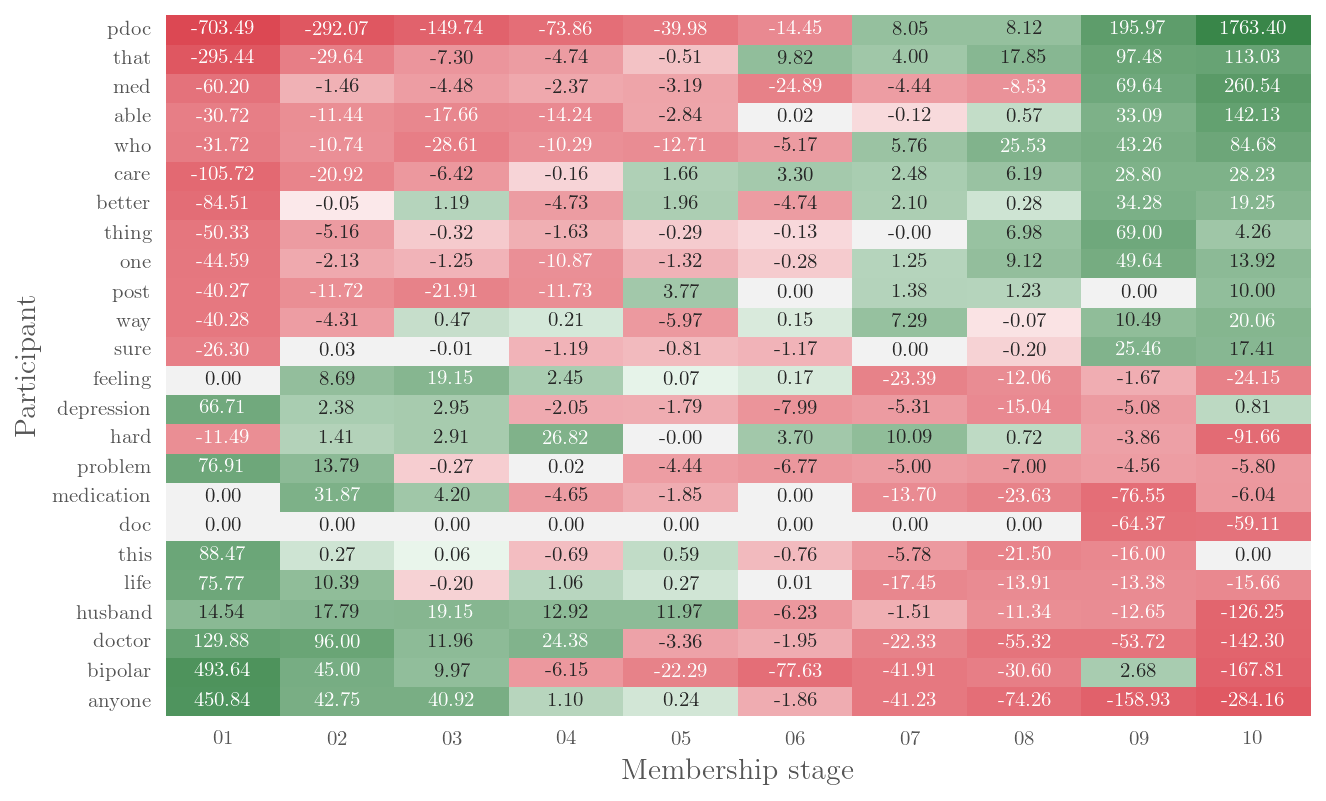
\includegraphics[width=1\textwidth]{../images/symlog-part2}
    \caption[Keywords on increasing and decreasing trajectories]{Keywords on increasing and decreasing trajectories (symmetric logarithmic colour scale)}
    \label{fig:key-traj}
    \end{figure}

Exploratory concordancing of various lexical items in Table \ref{tab:keyunkey-threestage} and Figure \ref{fig:key-traj}, revealed four key \glspl{theme}: \emph{jargonisation}, \emph{metadiscourse}, \emph{vague language} and \emph{the construal of instability}. These \glspl{theme} are explored in the sections below. 

\subsection{Jargonisation} \label{sect:jargon}

% Jargon term use by postcount
\begin{figure}[htb]
    \begin{center}
    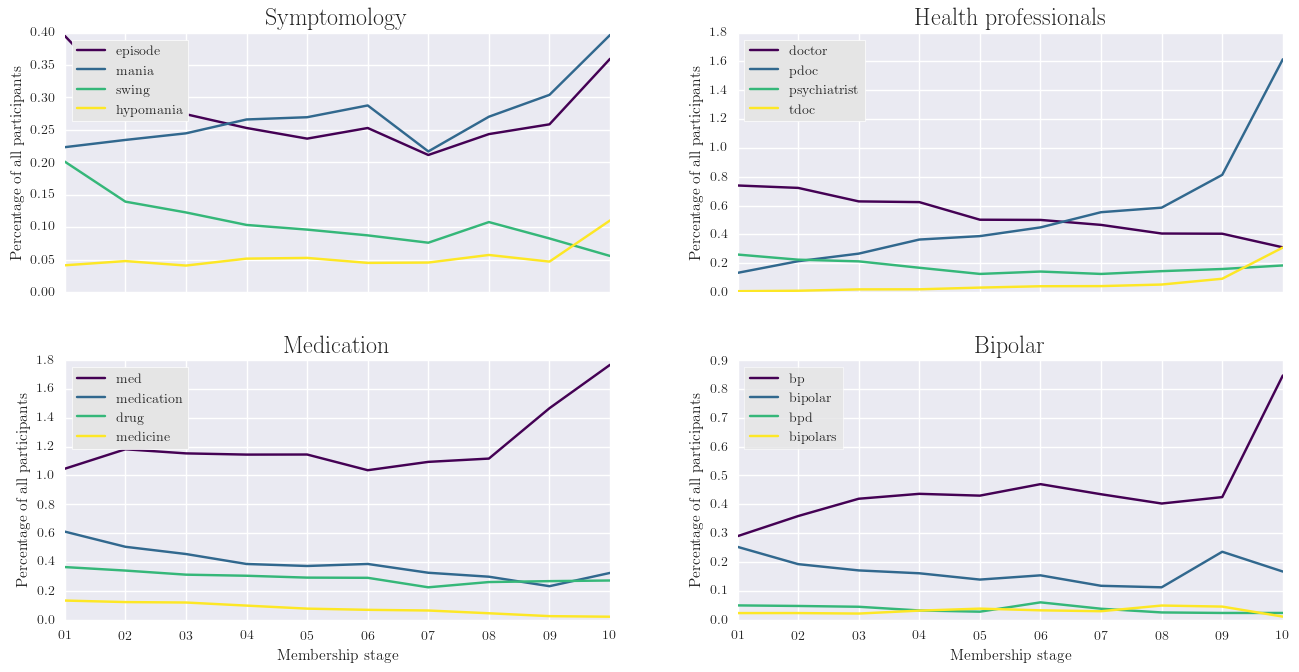
\includegraphics[width=0.90\textwidth]{../images/better_jargon.png}
    \end{center}
    \caption{Jargon term use by postcount}
    \label{fig:jargon}
    \end{figure}

The first theme of interest based on participant frequencies is jargonisation. In systemic\hyp{}functional terms, jargon serves important roles within both interpersonal and experiential metafunctions. Interpersonally, jargon demonstrates familiarity with community norms and expectation \cite{martin_language_2005}, and can demonstrate a (lay) expertise that enhances legitimacy. Experientially, jargon can also achieve more delicate distinctions between important participants in a given Field of discourse: the shift from construal of \emph{mood swings} to states of \emph{mania and hypomania} highlight the potential for jargon to facilitate more advanced taxonomisation of \gls{bipolar} and its symptoms.

Over the course of membership, jargon becomes significantly more common: \emph{meds}, \emph{pdoc}, \emph{tdoc}, \emph{bp} and \emph{mania} are all \gls{Forum} jargon, all featuring and within most key participants in late stages of membership (Table \ref{tab:keyunkey-threestage}) and the top ten participants in veteran \gls{member} talk in terms of relative frequency. Jargon terms also steadily displace non\hyp{}jargon variants: \emph{medication} becomes \emph{med(s)}, and \emph{bipolar} becomes \emph{bp}. Figure \ref{fig:jargon} shows this pattern in four subcomponents of the Field of discourse overall. Within symptomatology, \emph{mood swings} decrease, as discussion of \emph{mania} and \emph{hypomania} emerge. Terms for health professionals are shortened: psychiatrist and doctor become \emph{pdoc} at later stages. For medication, \emph{Med(s)} rises in frequency while \emph{medication} and \emph{drug} decline. For Bipolar Disorder itself, veteran members show a dramatic shift in preference toward \emph{bp}. Interestingly, some changes are multi\hyp{}stage: Figure \ref{tab:key_part_w_prop} shows how \emph{doctor} becomes \emph{doc} in middle stages, before finally splitting into \emph{pdoc} and \emph{tdoc} in late stages.

A final point to note here is that the relationship between participant and lexical item is not perfectly one\hyp{}to\hyp{}one, as many agnate terms (often in the form of jargon) exist at different stages of membership to denote the same Thing. Therefore, to more accurately gauge shifting Fields of discourse, it is necessary to attempt at least a basic collapsing of participant taxonomies, and of jargonised and non\hyp{}jargonised terms. This is performed later in the chapter.

\subsection{Metadiscourse}

% problem: the examples aren't participants!
%todo: help interpreting the figure
As can be seen in Figure \ref{fig:metadiscourse}, \emph{board} and \emph{group} are the main way that members refer to the community itself (0.044 and 0.065 per cent of all participants, compared to \emph{forum} at 0.009 per cent). \emph{Board} and \emph{group} become more frequent over the membership course, as do other terms that denote features of the \gls{OSG} such as \emph{post} and \emph{thread}. While new \glspl{member} typically commend the \glslink{Forum}{board} and explicitly mark the fact that they have recently found it, veteran \glspl{member} speak on its behalf and outline its goals and orientation (see Table \ref{tab:board} for instances of \emph{board}, not limited to participant roles). Over the course of membership, \glslink{member}{users} thus increasingly construe the community as a Thing that can bring about Events and Goals. Most importantly, the \gls{Forum} is capable of acting \emph{for} \glslink{member}{users} in the service of providing information and support. Construal of the \gls{Forum} as a static entity acted upon by its \glspl{member}, or as a non\hyp{}essential circumstance of location, decreases over time.

% Key metadiscourse words
\begin{figure}[htb]
    \begin{center}
    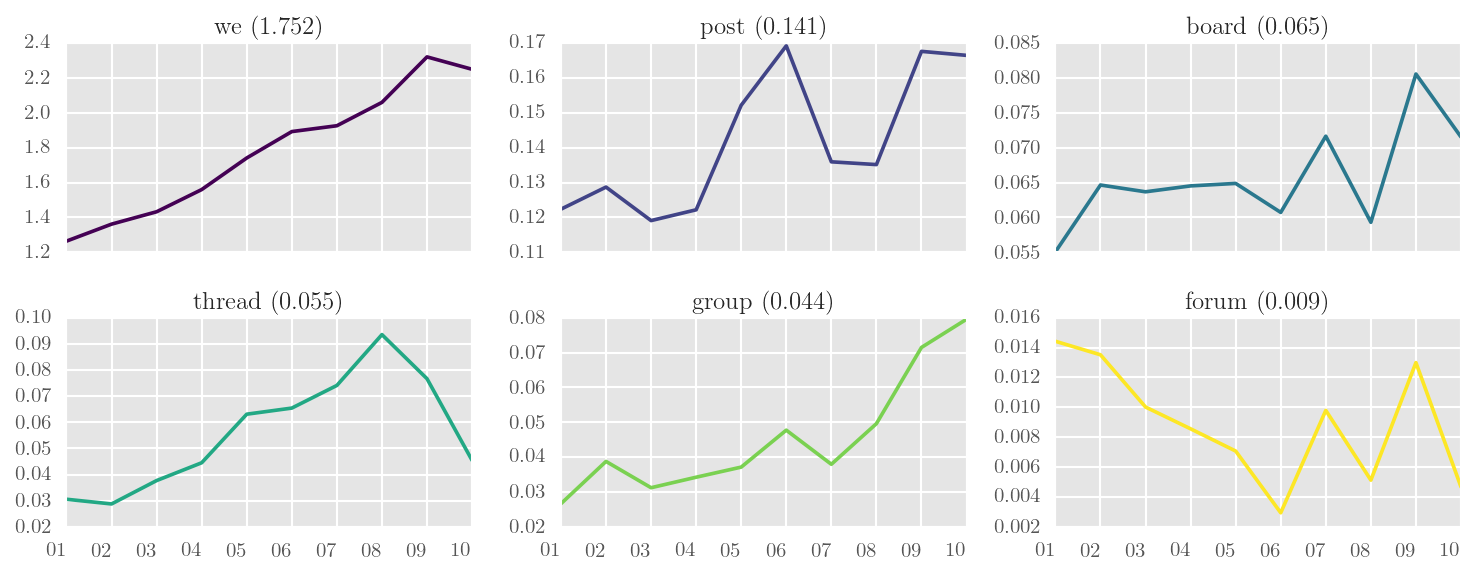
\includegraphics[width=0.70\textwidth]{../images/subplot-metad.png}
    \end{center}
    \caption{Key metadiscourse words}
    \label{fig:metadiscourse}
    \end{figure}


% References to \emph{board} in new and veteran talk
\begin{figure}[htb]
    \centering
    %\minipage{0.44\textwidth}\centering
    \begin{tabular}[t]{@{}>{\raggedright\arraybackslash}p{0.45\textwidth}}
    \vspace{1mm}
    New users
    
    %\noindent\parbox[t]{0.44\textwidth}{\raggedright%
    \begin{enumerate} [before=\itshape,font=\normalfont] \setlength\itemsep{0em} \footnotesize
    %\item Keep talking and being patient ... it will happen but it isn't going to happen overnight like we all would like it too.
    \item I'm so happy to have found this \textbf{board}.
    \item I'm not new to the \lbrack website\rbrack, but new to this \textbf{board}
    \item Thanks for this \textbf{board}, everyone's \glspl{post} have been really helpful to read.
    \item I am hopeful regarding being on this message \textbf{board} and sharing with all of you.
    \item i just joined this message \textbf{board}.
    \end{enumerate}
    \end{tabular}
    \begin{tabular}[t]{@{}>{\raggedright\arraybackslash}p{0.5\textwidth}}
    \vspace{1mm}
    Veteran users
    
    \begin{enumerate}[before=\itshape,font=\normalfont] \singlespacing \setlength\itemsep{0em} \footnotesize
    \item I'm glad you told him about the \textbf{board} and about NAMI.
    \item Part of the purpose of the \textbf{board} is for venting.
    \item Hello, Welcome to the \textbf{board}.
    \item on this \textbf{board} at least , pdoc is psychiatrist and tdoc is shorthand for therapist...
    \item Your sage comments are missed by all on the \textbf{board}.
    \end{enumerate}
    \end{tabular}
    %\endminipage
    \caption{References to \emph{board} in new and veteran talk}
    \label{tab:board}
    \end{figure}
%
\noindent Though experiential meanings, strictly speaking, construe information about events in the world, rather than role\hyp{}relationships between participants in interactions \cite{eggins_introduction_2004}, salient role\hyp{}relationship negotiation is performed through the differing discursive function of metadiscourse according to membership length. New \glspl{member}' discussion typically highlights the division between the \glslink{Forum}{community} and the self (\emph{I'm so happy to have found this board}), whereas veteran \glspl{member} construct a shared identity with the \glslink{Forum}{board} (\emph{Hello, welcome to the board}). Further, only veteran talk about the board is elaboratory or explanatory (\emph{Part of the purpose of this board is for venting}).

Also shown in Figure \ref{fig:metadiscourse} is that the use of \emph{we} increases over the course of membership. Concordancing of Subcorpus 10 shows that \emph{we}, like \emph{board} and \emph{group}, commonly occurs during explanation of the function(s) of the \glslink{Forum}{community} to newer \glspl{member}. As can be seen in Figure \ref{fig:we_conc}, another common use of \emph{we} in veteran talk is in generalisations about the lived experience of all people living with \gls{bipolar}---a discursive strategy that simultaneously stakes a claim to knowledge about bipolar and highlights the role of lay\hyp{}experience as the source of this knowledge.

%Two functions of \emph{we} in veteran users' language
\begin{figure}[htb]
    \centering
    %\minipage{0.44\textwidth}\centering
    \begin{tabular}[t]{@{}>{\raggedright\arraybackslash}p{0.45\textwidth}}
    \vspace{1mm}
    \begin{enumerate} [before=\itshape,font=\normalfont] \singlespacing \setlength\itemsep{0em} \footnotesize
    \item Hang in there and know that \textbf{we} are all rooting for you.
    \item Keep on venting and taking one thing at a time and know that \textbf{we} are here.
    \item So what happened, {[}username{]} ... \textbf{we} were soo worried about you the other night.
    \item None of us can diagnose you since \textbf{we} are n't medical professionals, but it very well could be bipolar.
    \item Also remember that \textbf{we} are all here for you anytime you need us.
    \end{enumerate}
    \end{tabular}
    \begin{tabular}[t]{@{}>{\raggedright\arraybackslash}p{0.45\textwidth}@{}}
    \begin{enumerate}  [before=\itshape,font=\normalfont] \singlespacing \setlength\itemsep{0em} \footnotesize
    \item For whatever reason, \textbf{we} want to think that the brain \textbf{we} were born with is just fine thank you very much.
    \item With bipolar disorder the rock does edge off of us - it just seems to take forever and \textbf{we} are so powerless beyond our meds to make it go away.
    \item I think sometimes \textbf{we} are just too overwhelmed to act.
    \item I think part of the reason \textbf{we} crash is that \textbf{we} are simply exhausted.
    \item For after all, \textbf{we} are all the sum total of our experiences.
    \end{enumerate} 
    \end{tabular}
    \caption{Two functions of \emph{we} in veteran users' language}
    \label{fig:we_conc}
    \end{figure}

\subsection{Vague language} 

The appearance of \emph{thing} as an increasingly prominent participant in veteran talk warranted further analysis. Initially, lemmatisation had conflated \emph{thing} and \emph{things}, with the latter being the site of the most change. Concordancing of \emph{things} in new \gls{member} \glspl{post} showed that \emph{things} often described past circumstances (\emph{things were getting really bad}). In contrast, veteran \glspl{member} used \emph{things} in expressions of general support (\emph{things will get better!}): % (see Figure \ref{fig:things}). 

%todo
%things as subject as perc of subjects / things not as subject as perc of non-subjects
% things as subject in present tense / things as subject in past tense

% things
\begin{enumerate} [before=\itshape,font=\normalfont] \singlespacing \setlength\itemsep{0em} \footnotesize
    %\item   \textit{\textbf{things} will get better}
    \item  I hope  \textbf{things} improve for you soon
    %\item  I really hope \textbf{things} go well for you
    \item  I am glad that  \textbf{things} are looking up for you too
    \item  call your pdoc if  \textbf{things} do not improve very soon!
    %\item  put on a brave face during the times when \textbf{things} seem so great
    \item  decided to hold off a semester until you get \textbf{things} more under control
    %\item  Let us know how  \textbf{things} go.
    %\item  perhaps it will be your opportunity to turn \textbf{things} around
    \item  as soon as you get back on your meds \textbf{things} will be better, just wait and see!!!
    %\item  want to run away thinking that it will make  \textbf{things} better
    \end{enumerate}
%
To measure this difference, the tenses of clauses in which \emph{things} takes the position of experiential subject (generally Actor, but, more rarely, Sayer, Senser, or Token\slash Possessor) in new and veteran \glspl{member}' \glspl{post} were tallied. Figure \ref{fig:thingstense} shows that \emph{things} is more commonly used by new \glspl{member} to describe action in the past. In veteran talk, \emph{things} tends to be vague, and is more commonly focussed on the present and future. This change echoes the more general shift toward present tense, as outlined in the previous chapter. Though more in\hyp{}depth analysis is perhaps warranted, this feature in veteran talk could potentially be a strategy for providing advice that may be of benefit to the entire \glslink{Forum}{community}, rather than simply the \gls{thread} initiator. An alternative analysis is that \emph{things} may allow veterans to provide social support without the need to ask follow\hyp{}up questions. Given the high dropout rate of new \glslink{member}{users}, with most new \glslink{member}{users} \glslink{post}{posting} fewer than three times, requests for clarification of specific circumstances may often go unanswered. In order to complete more exchanges, advice is accordingly dispensed as soon as possible, with little clarification sought. Another manifestation of this strategy can be seen in Emz's reply to a new member in Chapter \ref{chap:introdata}: rather then attempting to clarify unexplained parts of the newcomers' narrative, Emz instead simply highlights that her beliefs and suggestions are based on incomplete information (\emph{From what you say, if sounds very likely that you might have Bipolar disoder}; \emph{If you're already seeing a psychiatrist [...], then find a different one}).

% Tense of clauses with \emph{things} as subject by postcount
%\begin{figure}[htb]
%    \begin{center}
%    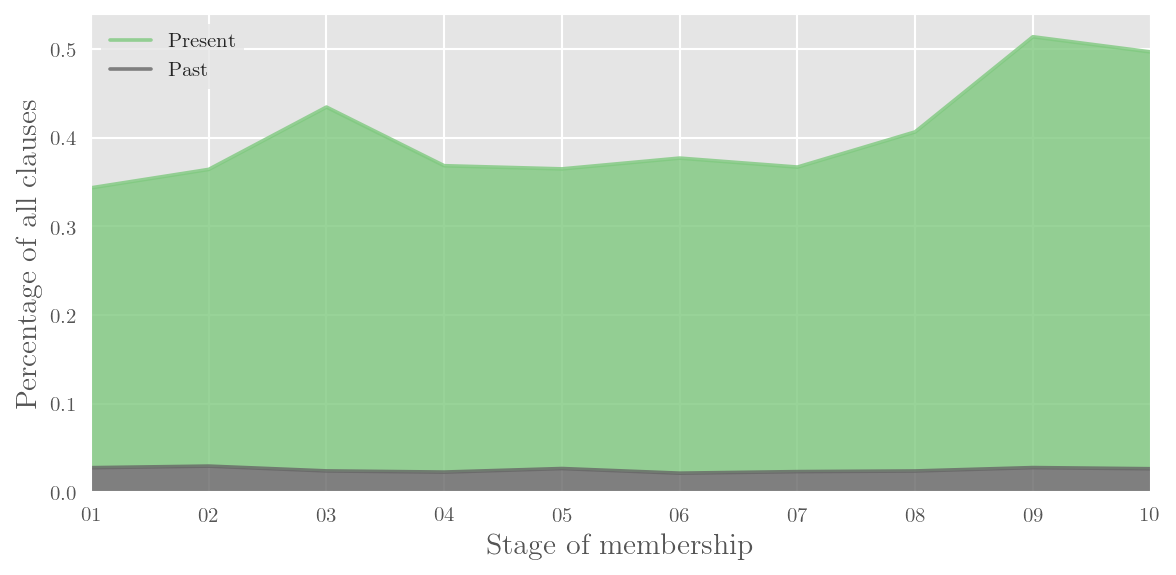
\includegraphics[width=0.70\textwidth]{../images/tense-things-new-area.png}
%    \end{center}
%    \caption{}
%    \label{fig:thingstense}
%    \end{figure}

\begin{figure}[htb]
    \minipage{0.48\textwidth}\centering
    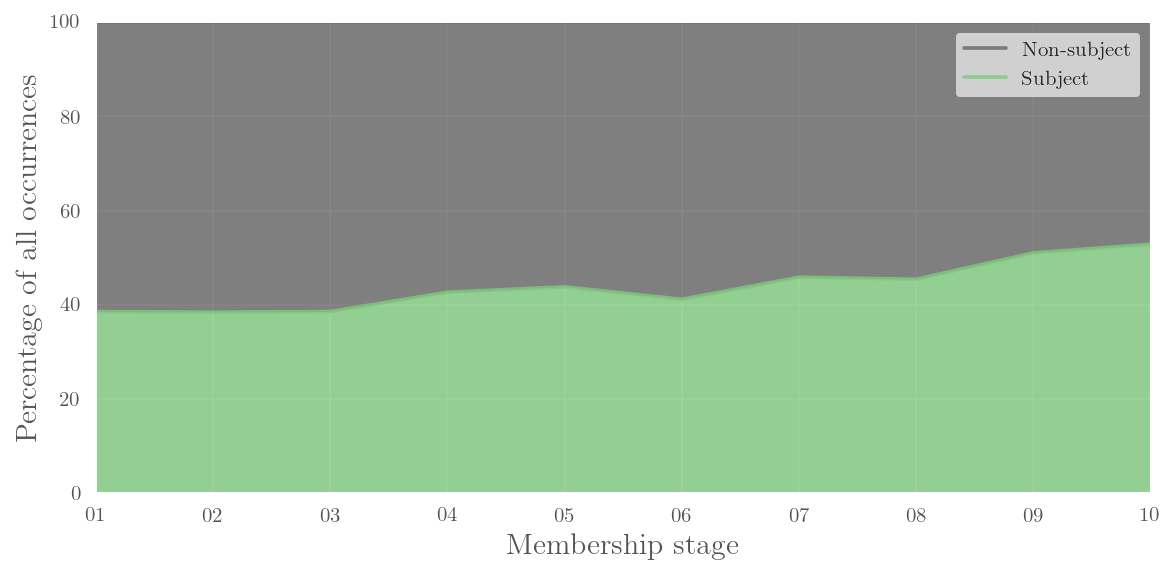
\includegraphics[width=1.00\textwidth]{../images/things-area.png}
    \endminipage\hfill
    \minipage{0.48\textwidth}\centering
    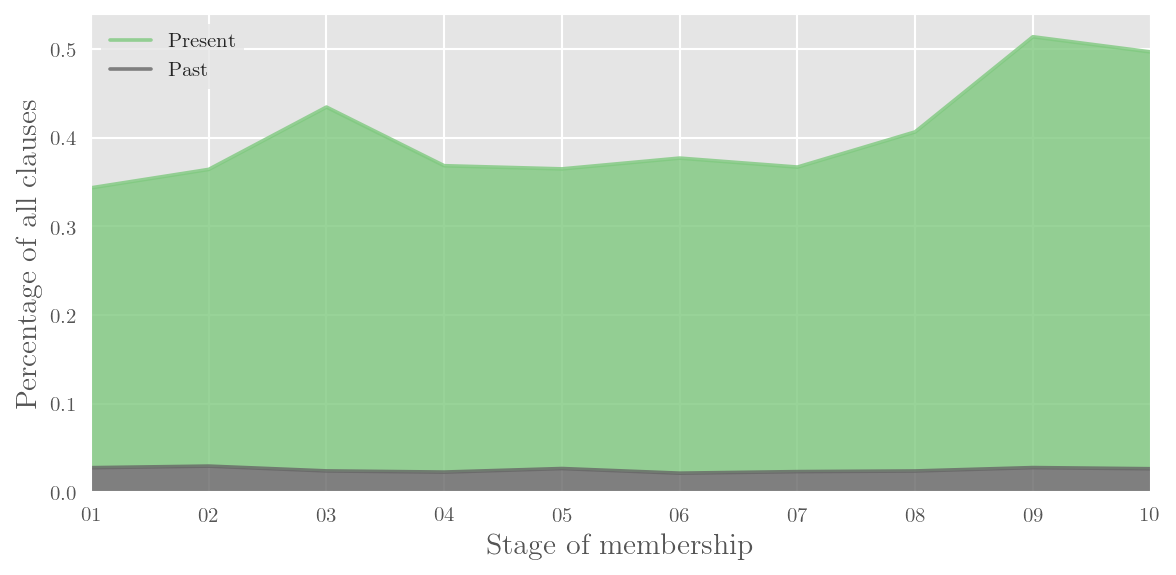
\includegraphics[width=1.00\textwidth]{../images/tense-things-new-area.png}
    \endminipage\hfill
    \caption[Increasing use of \emph{things}]{\emph{Things} as an increasingly common left participant, and as an increasingly common left participant in present tense clauses}
    \label{fig:thingstense}
    \end{figure}

\FloatBarrier
\subsection{Construing (in)stability}

Other results highlight changes in experiential semantics that can be mapped to the ideological orientation of the \glslink{Forum}{community}. One striking pattern evident in Table \ref{tab:keyunkey-threestage} is that newer \glspl{member} commonly construe negative mental states and desires that index instability and volatility (\emph{swing, angry, scared, crazy, kill}, etc.). For veterans, such terms are unkey, being reconfigured under an attitudinally neutral or potentially medicalised nominalisation, \emph{imbalance}. As seen in the qualitative analysis and noted in related literature \cite[e.g.][]{horne_doing_2009}, new \glspl{member} produce medical narratives connoting urgency in order to legitimate their membership bid and elicit responses. The framing of bipolar symptoms in emotive language, however, is dispreferred, with veteran \glspl{member} avoiding attitudinal lexis in favour of a nominalisation, \emph{stability}, which is represented as the possible result of proper care.

\begin{table}[htb]
\centering
\begin{tabular}{rll}
\toprule
terms of making sure that she finds &  stability   &  .                                   \\
t your finding and maintaining your &  stability   &  as well .                           \\
are important as far as maintaining &  stability   &  .                                   \\
to try different avenues to achieve &  stability   &  .                                   \\
            that way you will reach &  stability   &  so much quicker .                   \\
 those of us who have finally found &  stability   &  for ourselves or our loved ones it  \\
lf so that you will be able to find &  stability   &  and identify the stressors and deve \\
               he has given me more &  stability   &  over 2 months than i 've had in 1.5 \\
our `` seasoned '' bper who has had &  stability   &  for over 35 years .                 \\
 between of something resembling `` &  stability   &  '' or `` normalcy . ''              \\

\bottomrule
\end{tabular}
\caption{\emph{Stability} in veteran posts}
\label{conc:stability}
\end{table}

%\endnote{Tregex queries: \thingspresent~ and \thingspast}~ %A final point of discussion here is the appearance of \emph{things} in the top participants in veteran talk (See Figure \ref{fig:things}). The abstract and interpretable nature of the term (like \emph{time}, \emph{years}, \emph{people} and \emph{life}) allows it to be easily applied to the circumstances of newcomers when, especially when many details aren't known to the veteran member

\subsection{Construing human agency}

%todo: flag methodology
Because jargonisation disperses the potential lexical realisations of participants, wordlists must be created that can collapse the distinction between participants with multiple realisations in lexis during the \gls{corpus} interrogation process. The main human participants \cite[or social actors---see][]{van_leeuwen_representation_1996} in the Field of discourse can be divided into four : \emph{The Self}, \emph{Other Members}, \emph{Friends\slash Family} and \emph{Health Professionals}, with wordlists developed to match jargonised and non\hyp{}jargonised variants (Table \ref{tab:hum_part_lex_real}). For the remainder of the thesis, these capitalised terms denote the results of the four search queries, while lowercase variants refer to the social actor in general. Of course, such an approach means that many instances will go uncaptured, due to grammatical metaphor, misannotation, pronominalisation and so on. Even so, there is sufficient data for exploring how these four participant types behave over the membership course. Figure \ref{fig:part-tax-rel-freq} shows the relative frequency of four kinds of human participants over time. Clearly, Other \glspl{member} come to steadily displace the self as the ideational social actor being represnted. Friends and family, meanwhile, are on an uneven trajectory, occupying a larger part of the semantic space in early and late stages of membership than in the middle. Construal of health professionals rises dramatically in the late stages of membership. %The findings concerning Self and Other are in line with previous interrogation results. Collapsing jargon variants of terms for health professionals, however, has allowed us to see the overall rise in construals of health professionals as participants over the membership course. 

\begin{table}[htb]
    \centering
    \small
    \begin{tabularx}{\textwidth}{lX}
    \toprule
    Participant type & Realisations \\ \midrule
    The Self                & \emph{i}, \emph{myself}, \emph{me}            \\
    Other Members           & \emph{you}, \emph{yourself}, \emph{kat}, \emph{seaturtle}            \\
    Friends\slash Family    & \emph{friend}, \emph{mother}, \emph{husband}, \emph{daughter}, \emph{son}, \emph{wife}, \emph{father}, \emph{dad}, \emph{mom}, \emph{mum}, \emph{erin}           \\
    Health Professional     & \emph{doc}, \emph{docs}, \emph{doctor}, \emph{doctors}, \emph{dr}, \emph{dr.}, \emph{drs}, \emph{g.p.}, \emph{gp}, \emph{gps}, \emph{nurse}, \emph{nurses}, \emph{pdoc}, \emph{pdocs}, \emph{psych}, \emph{psychs}, \emph{shrink}, \emph{shrinks}, \emph{tdoc}, \emph{tdocs}           \\ \bottomrule
    \end{tabularx}
    \caption{Human participants and lexical realisations}
    \label{tab:hum_part_lex_real}
\end{table}

\begin{figure}[htb]
    \centering
    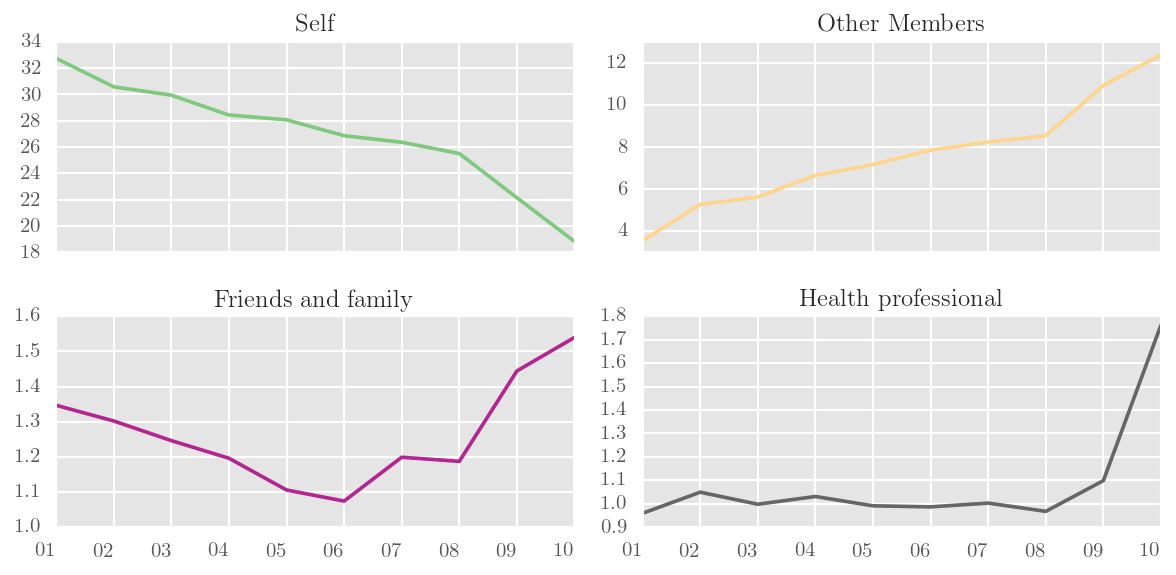
\includegraphics[width=0.8\textwidth]{../images/part-tax-rel-freq.png}
    \caption[Frequencies for four participant types]{Relative frequency of four participant types over the course of membership}
    \label{fig:part-tax-rel-freq}
    \end{figure}

Next, the ergative model of \sctext{Transitivity} can be used to determine the extent to which these human participant types are construed as Agents, and how this shifts with membership length. To measure this, each occurrence of participant type occuring in an Agentive dependency role can be divided by occurrences of the same participant type filling any participant role (Figure \ref{fig:key_proc_for_parts}). This controls for differences in the overall frequency with which certain participant types are mentioned.

Most notable in Figure \ref{fig:key_proc_for_parts} is the wide gap between health professionals and non\hyp{}health professionals in early contributions: when professionals are mentioned as participants in first \glspl{post}, they are in positions of experiential agency over 75 per cent of the time. Non\hyp{}health professionals, on the other hand, are more commonly positioned as Media---that is, as the entity through which a process comes into being. This is a representation of a world where health professionals are granted more control over medical processes than healthcare \glspl{consumer}, and where change in the world is enacted through the consumer, who may be willing or unwilling: patients are treated by doctors; doctors tell patients how to manage their condition. 

The clearest individual trend is the increasing agency granted to \gls{Forum} \glspl{member} generally. Veteran \glslink{member}{users} construct a discourse of \gls{consumercentred}ness by positioning their interlocutors as able to actively make changes in their inner and outer states. This method also makes it possible to see, for the first time, an increasing agency of The Self within the Field of discourse. Though The Self is less often charged with ensuring the completion of the clause as an intersubjective proposition (a responsibility increasingly delegated to the addressee), The Self is increasingly positioned as an entity that can bring about change in the world. Finally, there is a modest decrease in the proportion of \emph{Health\hyp{}professional\hyp{}as\hyp{}Agent} over membership length, closing an ideological divide present in early contributions, where health professionals carry out processes through the medium of the sufferer.

\begin{figure}[htb]
    \centering
    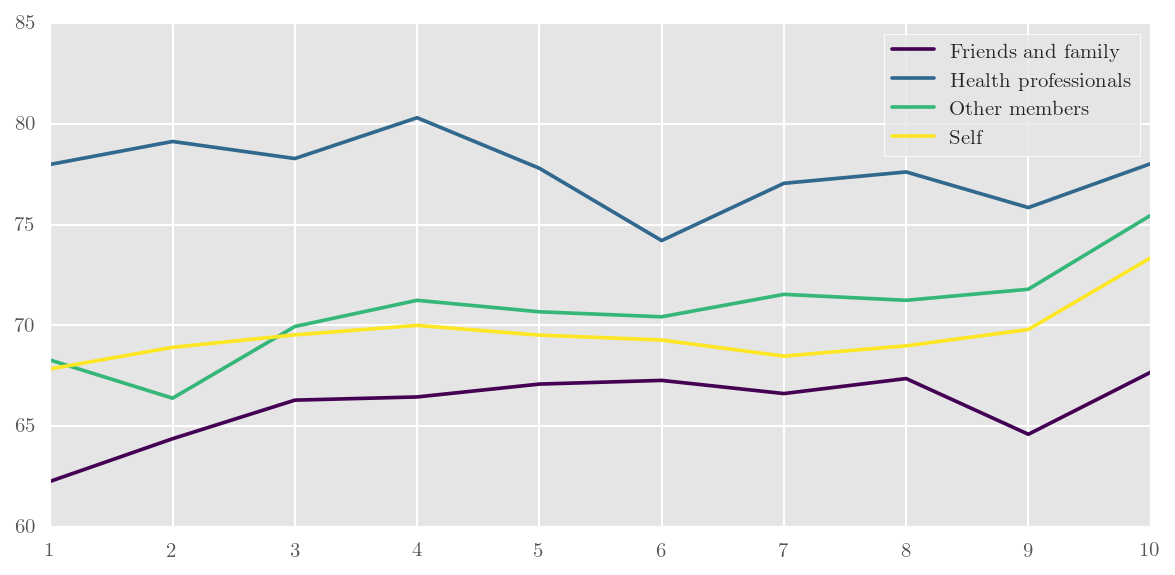
\includegraphics[width=0.85\textwidth]{../images/percentage-agent.png}
    \caption{Proportion of each participant type in Agent role}
    \label{fig:key_proc_for_parts}
    \end{figure}

%The notion of left-participant, however, is semantically very muddy, as participant roles are conflated. This is an unfortunate consequence of the fact that the Universal Dependency grammar does not distinguish between Agent and Medium, except in rare cases, such as passives with a \emph{by}-headed PP.

\section{Key processes} 

The next focus of the analysis of \sctext{Transitivity} choices is on processes, as typically realised by verbal groups at least one nominal group argument. Initially, we are interested in the head of this Process, which corresponds to the Event in the \gls{SFG}. In a constituency grammar, this is generally the rightmost verb in a VP; in the Universal Dependency grammar, Events are annotated with \emph{ccomp}, \emph{cop}, \emph{advcl} and \emph{root} labels. Therefore, an analysis of processes can begin in the same way that the analysis of participants was carried out, but with process\hyp{}like labels substituted for participant\hyp{}like ones.

% Key and unkey Events in each subcorpus
\begin{figure}
    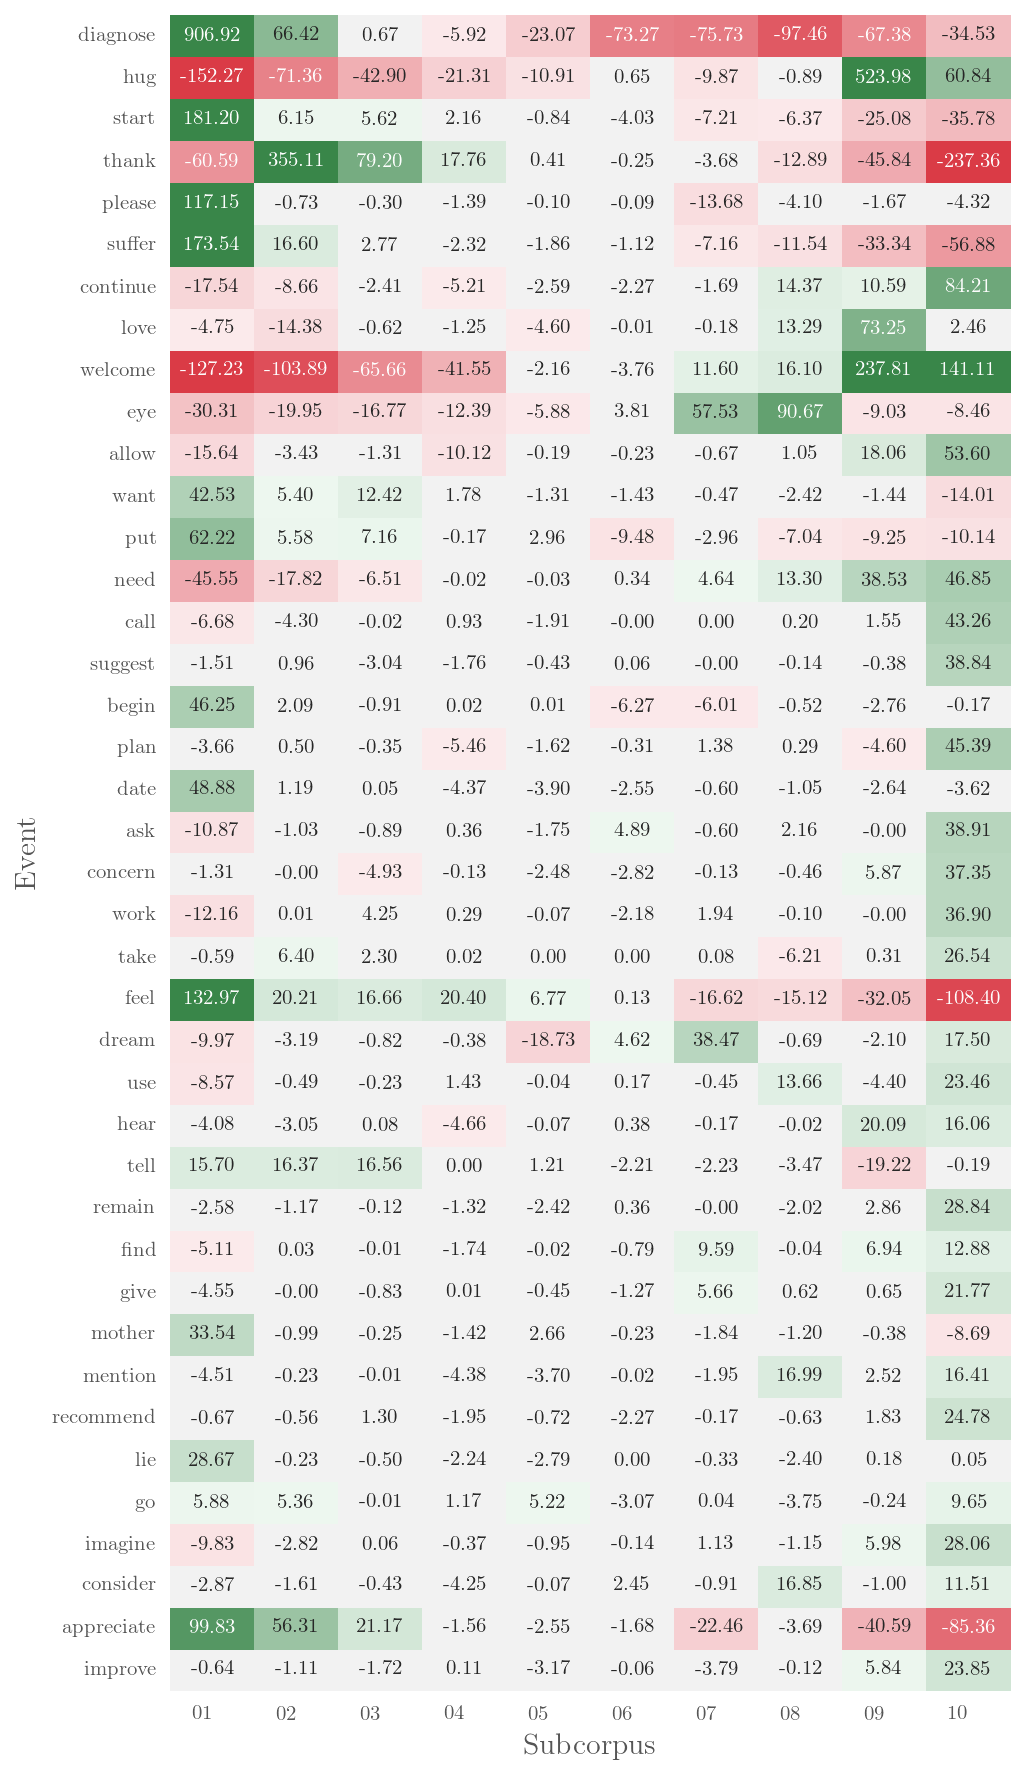
\includegraphics[width=0.80\textwidth]{../images/event-heatmap.png}
    \hspace{1.6cm}
    \caption{Key and unkey Events in each subcorpus}
    \label{fig:event_heatmap}
    \end{figure}

Figure \ref{fig:event_heatmap} shows which Events are key in each subcorpus according to a log\hyp{}likelihood comparison of the \gls{Forum} contents as a whole. By far the most key process in any subcorpus is \emph{diagnose} in Subcorpus 01, as diagnosis is both the catalyst for visits to the site, and the main entry condition for participatory information and support exchange. Similarly, \emph{thank} is key in second \glspl{post} because \glslink{member}{users} thank others for replies to their first. Other key Events in first \glspl{post} reveal other kinds of motivations for joining the \glslink{Forum}{community}, including being \emph{told} that they may have \gls{bipolar}, \emph{dates} with \glslink{bipolar}{bipolar} people, and \emph{beginning\slash starting} new medication regimens or manic\slash depressive cycles.

As with the analysis of participants, where veteran \glspl{member} orient toward more positive lexis, positive processes related to social support also become more common in veteran \glspl{post} (\emph{hug, thank, love, welcome}). Another focal point is processes urging others to carry on (\emph{continue, remain, improve}), which also have positive connotations. This contrasts with the negative sentiments inherent in \emph{suffer} (as in, \emph{to suffer from bipolar}), which is key in first \glspl{post} (see below for a more thorough treatment of the ways in which bipolar is ascribed to the self and others across membership stages). Finally, it is notable that \emph{thank} and \emph{appreciate} are unkey in the final stage of membership; the increased social status in the \glslink{Forum}{community} means that platitudes, for veterans, are no longer obligatory to the same extent.

\subsection{Construing diagnosis} \label{sect:diag}

%Concordancing allows a window into the figures involving \emph{diagnose} in early and late stages of membership.

% Goal of \emph{diagnose} processes in three stages of membership
% Circumstances in \emph{diagnose} processes in three stages of membership
\begin{figure}[htb]
    \centering
    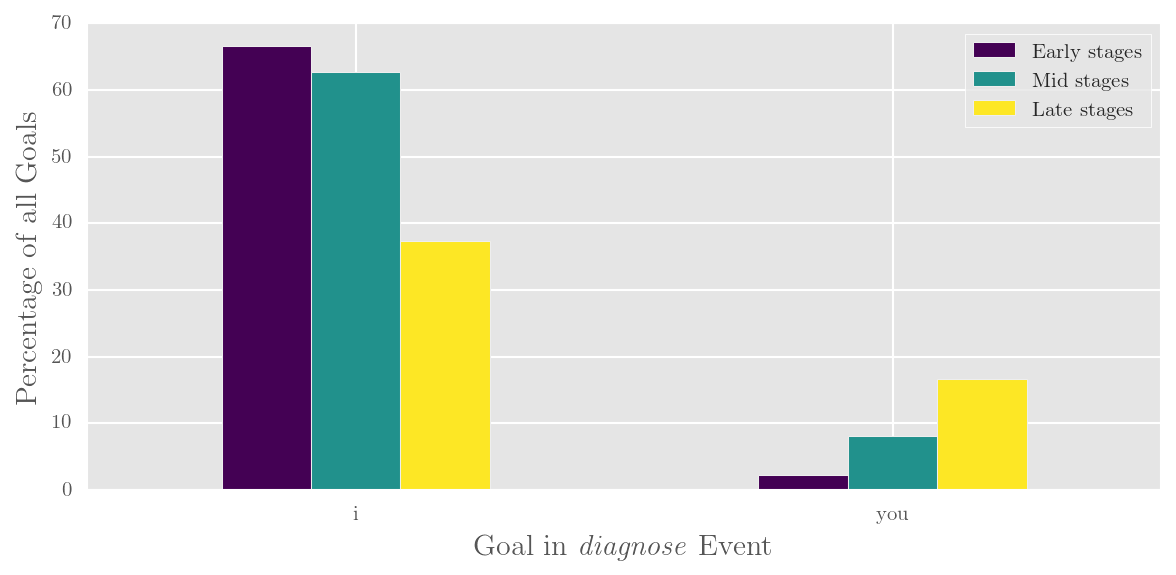
\includegraphics[width=0.8\textwidth]{../images/goal-in-diag-ev.png}
    \caption[Goal of \emph{diagnose} processes]{Goal of \emph{diagnose} processes in three stages of membership}
    \label{fig:part_in_diag}
    \end{figure}

    \begin{figure}[htb]
    \centering
    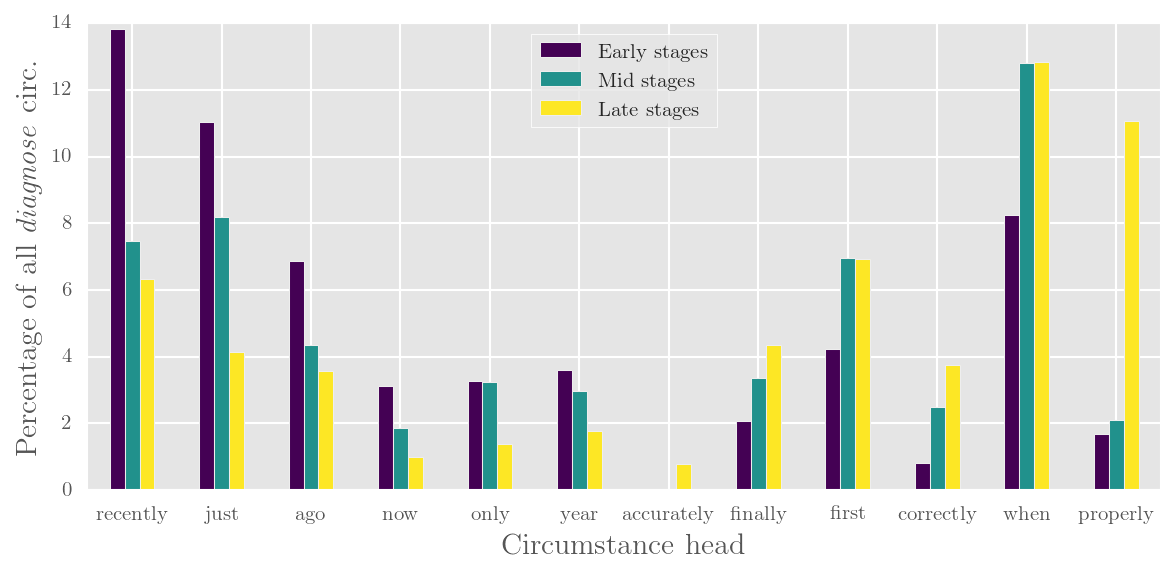
\includegraphics[width=0.8\textwidth]{../images/diag-circ.png}
    \caption[Circumstances in \emph{diagnose} processes]{Circumstances in \emph{diagnose} processes in three stages of membership}
    \label{fig:circ_in_diag}
    \end{figure}

\emph{Diagnose} is a very prominent process in the \gls{Forum}, and is by far the most key of key processes expressed in first \glspl{post}. By contrasting early, middle and late stages of membership, clear differences emerge in how the process of diagnosis is configured over time (Figure \ref{fig:part_in_diag}). Veteran \glspl{member}, for example, are more likely to represent the health professional as the Actor in the \emph{diagnose} process. In terms of circumstances (Figure \ref{fig:circ_in_diag}), there is a shift in focus away from temporal meanings, with veteran \glspl{member} instead framing the \emph{diagnose} process with regard to its correctness, accuracy and legitimacy. New \glspl{member} often enter the community because of a recent or possible future diagnosis. Veterans, on the other hand, seek to ensure that the diagnosis is reliable. This has the dual purpose of ensuring the legitimacy of the new member's `entry ticket', and ensuring conformance with the biomedical model, where successful treatment is predicated on accurate diagnosis. Indeed, a number of \glslink{member}{users} enter the community not because of a diagnosis from a health professional, but because they are attempting to ascertain whether their self\hyp{}diagnosis, or their informal diagnosis of a friend or loved one, can stand up to the scrutiny of lay\hyp{}experts. Veteran members, however, are reluctant to legitimise these kinds of strategies, due to their deviation from a normative conceptualisation of the `correct' consumer journey.

%Furthermore, they frame diagnosis as possibilistic: diagnoses can be \emph{suspected} or \emph{unofficial}. Such a framing is at odds with the normative biomedical model, however: informal kinds of diagnosis cannot be acted upon with appropriate treatment regimens. Veteran \glspl{member} therefore stress correct diagnosis in order to realign new \glspl{member}' construal of diagnosis with the ideology of the \glslink{Forum}{board}.

%Though the focus of the community is on offering information and support for people with \gls{bipolar}, those without official diagnoses ultimately cannot be helped \cite{vayreda_social_2009}. Ideologically, validation of community membership is withheld until new members have aligned with a normative biomedical trajectory that foremost involves diagnosis by professionals operating within a formal healthcare institution.

Notably, veteran \glspl{member} may deliberately undermine the biomedical model of diagnosis. While expressing conviction that diagnosis must be performed by a qualified health professional, they may simultaneously hint that the newcomer is \emph{probably} bipolar, or that non\hyp{}bipolar diagnoses are in error. As was shown in the qualitative analysis in Chapter \ref{chap:introdata}, two separate replies to an undiagnosed newcomer relied upon the same lexicogrammatical means of hinting (\emph{It sounds like you might have bipolar to me}; \emph{if sounds very likely that you might have Bipolar disoder}), while nonetheless insisting on seeking diagnosis through mainstream channels (\emph{Find you a dr that can make a correct Diagnosis}; \emph{We aren't docs here and can't diagnose you}). As shown in the following section, in veteran--veteran interactions, health professionals' ability to correctly identify and treat people living with \glslink{bipolar}{bipolar} is occasionally into question. This keeps the membership entry point open for those who have initially failed to meet the core criterion of a legitimate diagnosis, while pushing undiagnosed, suspected \glslink{bipolar}{bipolar} \glslink{member}{users} toward actions that are in line with mainstream medical norms. %Help can be better provided once the condition is met.

\subsubsection{Diagnosis and grammatical metaphor}

Grammatical metaphor entails the use of one grammatical component to do the work that is congruently performed by another. Nominalisation is one of the most common examples \cite{simon-vandenbergen_grammatical_2003}. What is congruently an action, process or Event (e.g. to \emph{applaud}) may be reconstrued as a participant (\emph{applause}), allowing denser packaging of information. Turning the process into a participant also facilitates taxonomisation and classification: the lexical component of a nominal group may include Classifier, Epithet and Numerative, in addition to the Thing; in the verbal group, the only lexical component is the Event \cite{halliday_introduction_2004}. This kind of grammatical metaphor also opens up the reconstrued process to deixis. For these reasons, it is a key characteristic of scientific English \cite{halliday1999construing}. 

Over the course of membership, the process of diagnosis undergoes a steady shift toward metaphorical realisation as a participant. In formal terms, it is more often nominalised. Figure \ref{fig:diag-gram-met} shows the strong relationship, but inexact, relationship between nominalisation and grammatical metaphor in the case of diagnosis: nominal and participant realisations become more frequent, while verbal and process realisations decrease. Charting experiential roles shows us that \emph{diagnose} is not limited to participant and process roles: commonly, it is a part of a circumstance (\emph{we received more help in terms of diagnosis and treatment}) or modifies a Thing (\emph{it is extremely common for those with undiagnosed bipolar disorder to self medicate}). The increasing extents to which \emph{diagnose} is nominalised, and to which \emph{diagnose} is represented as something other than a process, demonstrate an important discourse-semantic shift. By moving away from \emph{diagnose\hyp{}as\hyp{}process}, it becomes possible to represent diagnosis as a possession, (\emph{it's great you have a final diagnosis and have started medication}), and therefore something that can be acted upon or thought of in a particular way (\emph{i finally feel like i've accepted my diagnosis}). Another possibility opened up by nominalisation is the potential for modification through Epithets (\emph{this is a frightening diagnosis, particularly if you don't know anyone who has it}). Classification of \emph{diagnosis} through adjectival modification is also made possible (\emph{accurate}\slash \emph{correct} diagnosis), but, of course, as shown in Figure \ref{fig:circ_in_diag}, agnate meanings can be made through circumstantial modification of diagnose as a process (\emph{accurately\slash correctly diagnosed}). A final grammatical affordance is that diagnosis as a participant in a relational process can highlight its potential to be incorrect (\emph{my current diagnosis is schizo\hyp{}affective disorder}; \emph{bp is becoming a catch-all diagnosis, frequently made by a well-meaning family doctor}). In this way, grammatical metaphor not only contributes to an increasingly scientised register, but also expands veteran members' ability to explain medical processes and their relationship to other members \cite{heyvaert_nominalization_2003}.

Calculating the relative frequencies of common modifiers of diagnose as verb (\emph{diagnose}, \emph{diagnosed}, \emph{diagnosing}) and diagnose as noun (i.e. diagnosis\slash diagnoses) clearly shows a preference for temporal modification of verbs and veracious modification of the nominal form.

%More generally, veterans may wish to invoke a scientised register, which 

% Grammatical metaphor in \emph{diagnosis}, via word classes and experiential roles
\begin{figure}[htb]
    \minipage{0.48\textwidth}\centering
    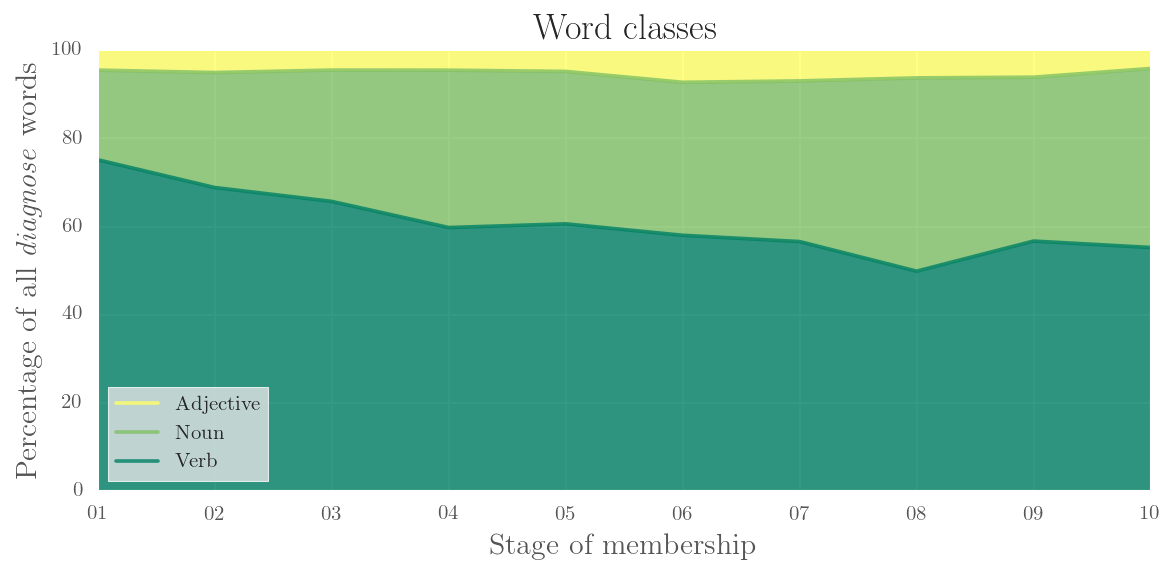
\includegraphics[width=1.00\textwidth]{../images/wc-diag.png}
    \endminipage\hfill
    \minipage{0.48\textwidth}\centering
    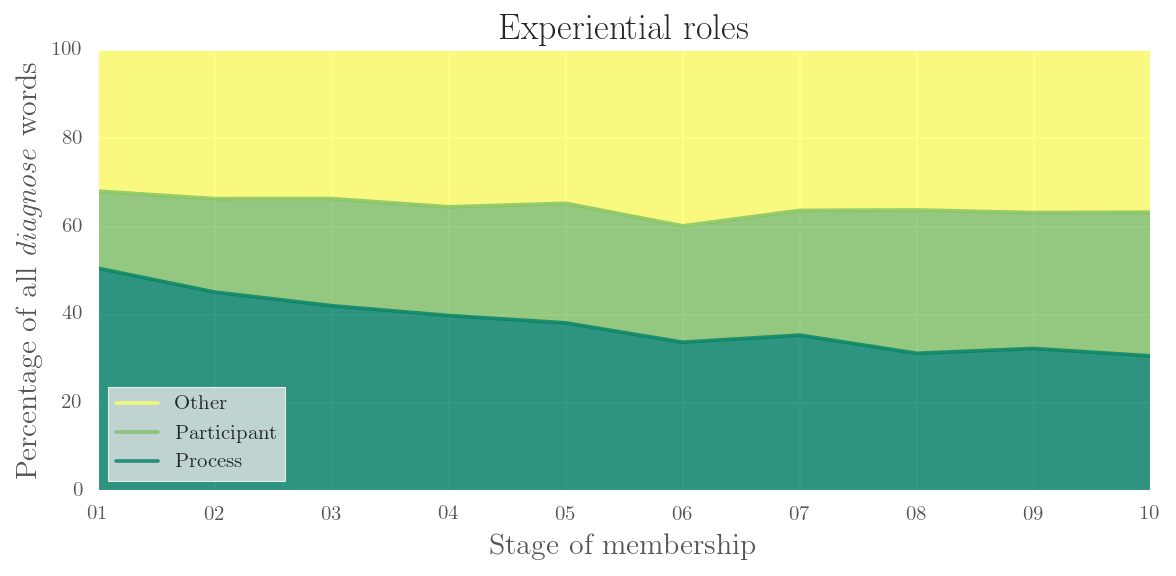
\includegraphics[width=1.00\textwidth]{../images/exp-diag.png}
    \endminipage\hfill
    \caption[Grammatical metaphor in \emph{diagnosis}]{Grammatical metaphor in \emph{diagnosis}, via word classes and experiential roles}
    \label{fig:diag-gram-met}
    \end{figure}

\begin{table}[htb]
\begin{tabular}{lrlr}

\toprule
\emph{Diagnose}  & Rel freq.        & \emph{Diagnosis} & Rel. freq. \\
\midrule
not               &  11.80 & bipolar    &  11.13 \\
ago               &  11.10 & proper     &   8.82 \\
just              &   7.60 & correct    &   7.49 \\
recently          &   6.68 & dual       &   5.07 \\
when              &   4.16 & right      &   4.41 \\
now               &   3.54 & new        &   3.96 \\
only              &   3.11 & official   &   2.75 \\
properly          &   2.75 & different  &   2.64 \\
also              &   2.27 & wrong      &   2.20 \\
finally           &   2.12 & other      &   2.20 \\
so                &   2.09 & same       &   1.87 \\
never             &   2.09 & initial    &   1.65 \\
then              &   1.93 & possible   &   1.54 \\
correctly         &   1.50 & true       &   1.54 \\
well              &   1.47 & recent     &   1.43 \\
\bottomrule
\end{tabular}
\caption{Most common modifiers of \emph{diagnose} and \emph{diagnosis}}
\label{relfreq-diagnose-mods}
\end{table}

%As could be expected, diagnosis is increasingly construed as a participant in the \Gls{forum}. By calculating the relative frequency of the diagnose process compared to processes generally, of diagnosis participants compared to participants generally, and diagnose words within other experiential roles, compared to other roles generally, we can see that diagnosis

% Interpretation?

\subsection{Construing the relationship between people and bipolar} \label{subs:behave}
    
As noted by \textcite{harvey_disclosures_2012}, people attribute depression to themselves in a number of different ways. The same set of grammatical constructions are available to those afflicted by many health issues, including \gls{bipolar}. In the \glslink{Forum}{Bipolar Forum}, people may \emph{have}, \emph{be}, \emph{feel} or \emph{suffer from} bipolar. For reasons of scope, however, only the two most common clause-level ascriptions---\emph{having} and \emph{being}---are examined in detail here, and group\slash phrase level ascriptions (i.e. \emph{a bipolar friend}) are not considered. To look for longitudinal changes in being\slash having constructions, the \gls{corpus} was interrogated for relational processes with bipolar (or jargon variants \emph{bp, bpi, bpii, bp1, bp2}, etc.) as a first object argument, and with human pronouns as the leftmost nominal group, returning lemma forms of the located relational Events.\endnote{Searching for participants by their order in clauses is often inaccurate, due to passivisation. In the case of relational processes, however, this is not an issue, as relational processes cannot be passivised (\emph{*bipolar was suffered from by me}).} Generated concordance lines were used to remove false positives caused by parser errors. Results were then recalculated from the concordance lines using \texttt{corpkit}'s \texttt{Concordance.calculate()} method.

%Lemmatisation was used to collapse the verb inflections for \emph{be}, \emph{have} and \emph{suffer}. Two kinds of false positives were discounted. First, clauses with \emph{it} as subject were excluded, as they were not ascribing bipolar to people, but explaining that bipolar is the cause of a certain symptom (e.g. \emph{It's probably the bipolar that makes you do that}).

% Processes with bipolar as Medium, combined
% Processes with bipolar as Medium, separated
\begin{figure}[htb]
  \begin{center}
  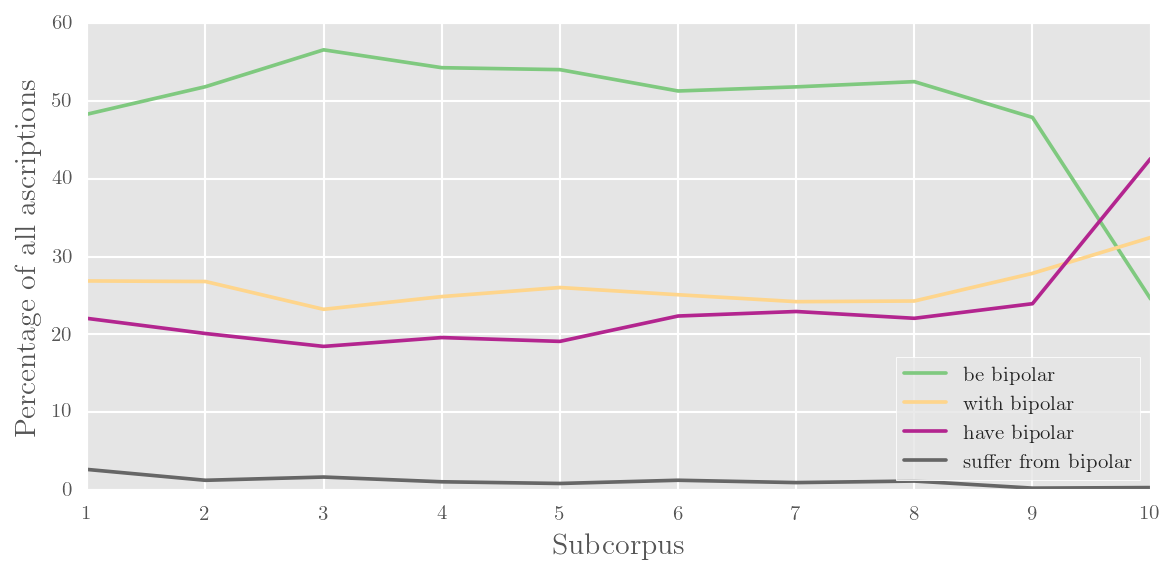
\includegraphics[width=0.75\textwidth]{../images/being_having.png}
  \end{center}
  \caption{Processes with bipolar as Medium, combined}
  \label{fig:behave}
  \end{figure}

  \begin{figure}[htb]
  \begin{center}
  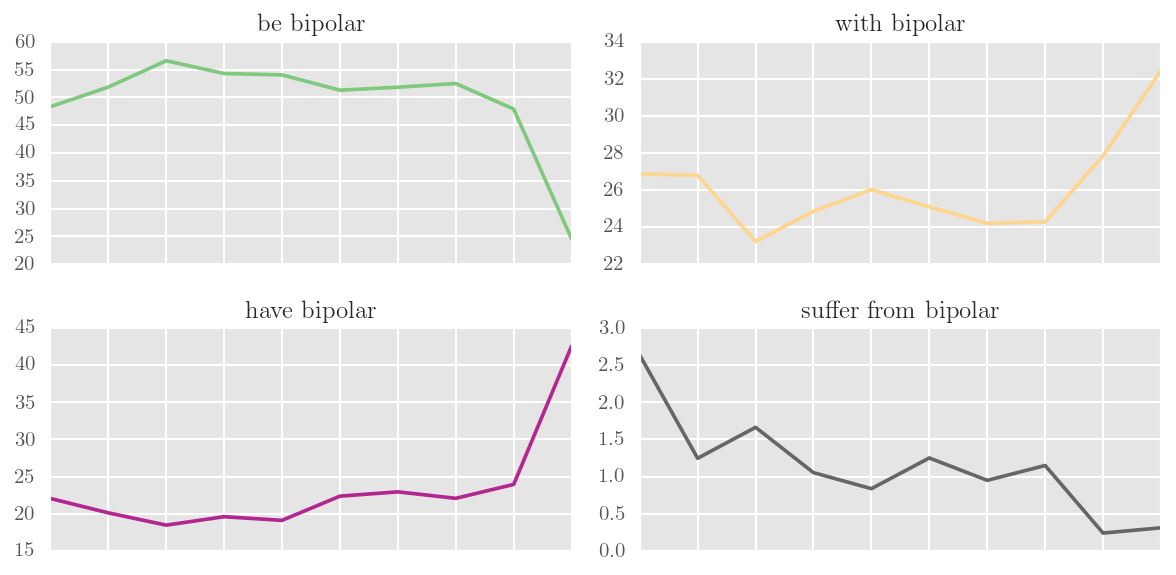
\includegraphics[width=0.75\textwidth]{../images/being_having_subplots.png}
  \end{center}
  \caption{Processes with bipolar as Medium, separated}
  \label{fig:behave_subplot}
  \end{figure}

Figures \ref{fig:behave} and \ref{fig:behave_subplot} show changes in the way \gls{Forum} \glslink{member}{users} construe the relationship between bipolar, themselves and others. Most strikingly, \emph{having} forms overtake \emph{being} forms as ways of ascribing \gls{bipolar} to the self and others. This change occurs very late in the membership course. Similar is the growth in attribution via circumstances, as in \emph{a person with bipolar}. To \emph{suffer from} \glslink{bipolar}{bipolar} decreases steadily over the course of membership.

Understanding these changes requires analysis of the grammatical properties of each kind of ascription. First, the shift away from \emph{suffering from} and \emph{feeling} is away from mental and toward relational processes. This shift includes the increasing frequency of attribution via \emph{with}, as grammatical circumstances are in fact partially articulated relational processes. Both \emph{being} and \emph{having} constructions are attributive relational processes, meaning that in both cases an attribute is ascribed on some level to the experiential subject. The difference is in the nature of the attribution. \emph{I have bipolar} is a \textbf{possessive attributive}, in which the experiential subject functions as a possessor of the attribute, which is inherently possessed. Possession itself is foregrounded in the process of having; ownership of bipolar is ascribed to the subject. Inversion of the clause highlights the dominance of the possessor over the possessed: \emph{bipolar has me} conveys an (undesirable) lack of control over the condition. \emph{I am bipolar}, on the other hand, is an \textbf{intensive attributive} construction, where bipolar forms a class in which the subject is a member. Halliday and Matthiessen's \citeyear{halliday_introduction_2004} use of the term \emph{Carrier} for the subjects in these kinds of processes highlights the ambiguity concerning the Carrier's willingness to be ascribed the attribute. This construct is ultimately dispreferred by veteran users, as it creates a subclass of person characterised chiefly by the ascribed bipolarity, rather than foregrounding the process of ownership, and, by extension, some control over their possessed condition.

The salience of the two constructions is evident in the fact that veteran \glslink{member}{users} of the \emph{Bipolar Forum} may explicitly draw attention to the \emph{being\slash having} distinction. Recalling the qualitative analysis of a new \glslink{member}{user}'s interaction with two more senior \glspl{member} (see Section \ref{sect:jess-post} for the complete reproduction), we can see that each interactant construes Jess as having \gls{bipolar} using different relational process lexis:

\begin{quotation}\small\singlespacing

\noindent \textbf{Jess}: [...] i have asked my doctor to test me to see if i am bipolar as my antidepressants do not work even though they have been changed a million times!! [...] i want to change my doctor and have been telling my partner i would but im scared of finding out that i am bipolar [...]

\noindent \textbf{Luvsoccer}: It sounds like you might have bipolar to me. You need to change Drs. One with more knowledge apparently. The reason the antidepessants are not Working is because If you are bi polar and they put U on an antidepressant alone it can make things worse... [...]

\noindent \textbf{Emz}: Hi, welcome to the boards, hopefully we can help you out and be a support system for you. First off you're not A bipolar, *l* we're not things, it's a condition. From what you say, if sounds very likely that you might have Bipolar disoder. [...]

\end{quotation}
%
Jess exclusively uses \emph{being} forms, while \emph{Luvsoccer} switches between \emph{having} and \emph{being}. Emz, however, uses only \emph{have} forms, except when explicitly drawing attention to the fact that copula ascription is dispreferred. To make this point, she highlights a potential reading of the \emph{being} construction as an \emph{intensive identifying} process, whereby the experiential subject has \emph{bipolar} assigned to it for the purposes of identification, rather than quality attribution. This is undesirable among the community: as explained by the veteran user, it is preferable to be a member of a class of \emph{people} possessing a particular quality of \emph{bipolar}, rather than a relationship of equivalence between the Identifier and Identified.

% A veteran user discussing the being\slash having distinction
\begin{figure}[htb]
  \centering
  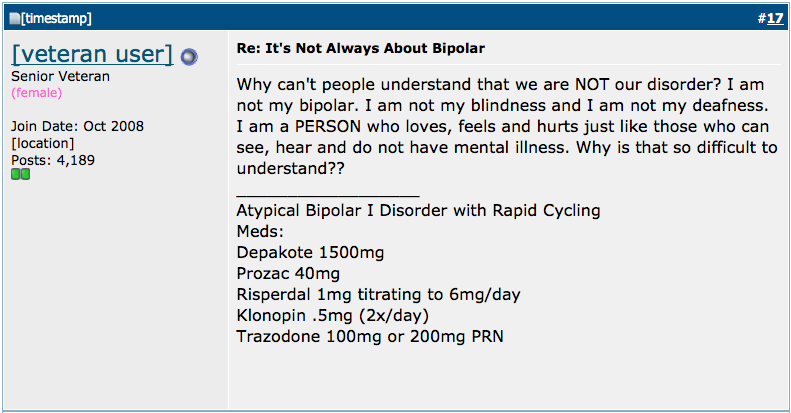
\includegraphics[width=0.60\textwidth]{../images/notourbipolar.png}
  \caption{A veteran user discussing the being\slash having distinction}
  \label{fig:notour}
  \end{figure}
%    
Some of the rare instances of \emph{being} constructions in Subcorpus 10 are in fact the result of veteran \glslink{member}{users} recasting new users' claims of \emph{being bipolar} as \emph{having bipolar}, as can be seen in Emz' response to Jess. Note the veteran's insertion (and capitalisation) of the indefinite article during her recast: \emph{First off, you're not \textbf{A} bipolar, we're not things}. Here, the veteran \gls{member} is highlighting a second potentially undesirable reading of the \emph{being} construction, where rather than functioning as an Epithet, \gls{bipolar} becomes a Thing. This transforms the attribute into an entity, rather than Quality, and renders the class of \glslink{bipolar}{bipolar} (as the veteran \gls{member} points out) a Thing to which a person can be equated, rather than a trait that may (currently) characterise someone.

%% Veteran recasting new user's copula constructions
%\begin{figure}[htb]
%  \begin{center}
%  \includegraphics[width=1.0\textwidth]{../images/newandreply.png}
%  \end{center}
%  \caption{Veteran recasting new user's copula constructions}
%  \label{fig:notabipolar}
%  \end{figure}

%Genre analysis (see below) suggests that new members' introductions to the community may be influenced by prior knowledge of generic norms in face\hyp{}to\hyp{}face support groups, such as \emph{Alcoholics Anonymous}, in which members use a well-known \emph{being} form when greeting one another (\emph{Hi, I'm \lbrack ~name \rbrack~ and I'm an alcoholic}). Though this influences the prevalence of being forms in first \glspl{post}, \emph{being} forms persist during the first stages of membership (see Figure \ref{fig:behave}).

Aside from recasts, in veteran \glspl{post}, however, \emph{being} constructions are exceptionally rare. In the highest postcount group, only 11 matches were found, with eight cases involving ascription to others, rather than the writer him\slash herself. One post, in which the self was identified as \emph{being} \glslink{bipolar}{bipolar} three times was selected for further analysis (Figure \ref{fig:firstsaid}).
    
%\endnote{The AA website explains that `Using the somewhat cliched AA introduction of ``Hi, my name is \lbrack name\rbrack~and I'm an alcoholic'' is not requirement but simply a custom adopted independently by many groups and members' \citeyear{_must_2014}}~
%\begin{quote}
%\small \singlespacing
%The pdocs at the first hospital said I was bp1. Then at the state hospital they said I was bp2, then they said I was schizoaffective bipolar type.
%\end{quote}

% A veteran user employs \emph{being} forms
\begin{figure}[H]
  \begin{center}
  \includegraphics[width=0.6\textwidth]{../images/firstsaid.png}
  \end{center}
  \caption{A veteran user employs \emph{being} forms}
  \label{fig:firstsaid}
  \end{figure}
%
\noindent Here, pivotally, it is pdocs, rather than the speaker himself, who (twice) invoke the \emph{being} construction, through an embedded clause in the Verbiage. Given that elsewhere in the forum the same member had employed \emph{having} constructions, analysis of entire threads was performed, in order to better understand veteran's motivations for using \emph{being} forms. In multiple cases, veterans appeared to use \emph{being} constructions to help establish a negative characterisation of the health professionals in the process of diagnosis. In an earlier \gls{post}, the \glslink{member}{user} had told the story of his misdiagnosis:
    
            %\begin{quote}
            %\small \singlespacing
            %If you can't be hypomanic and have psychosis, then why in the hospital did they change my diagnosis to bipolar 2 when I was clearly psychotic? They changed it that way because they said I have more problems with depression instead of mania. That was their reasoning.
    
            %\noindent Now my diagnosis is something different. I'm beginning to wonder if some of these pdocs even know what they are doing.
            %\end{quote}

% A veteran user's characterisation of pdocs as incompetent
\begin{figure}[H]
  \begin{center}
  \includegraphics[width=0.6\textwidth]{../images/incomppdocs.png}
  \end{center}
  \caption{A veteran user's characterisation of pdocs as incompetent}
  \label{fig:incomppdocs}
  \end{figure}
%
\noindent The writer's uses of the dispreferred \emph{being} constructions add weight to his positioning health professionals as incompetent: in the narrative, health professionals can neither offer correct diagnosis for their patients nor adequately conceptualise the relationship of ownership and possession between person and condition that functions as an important normative value in the \glslink{Forum}{community}.

\subsection{Process-participant type configurations}

Earlier, I analysed the frequency of four kinds of participants in the Forum's Field of discourse (\emph{The Self}, \emph{Other Members}, \emph{Health Professionals} and \emph{Friends\slash Family}, and the proportion of occurrences of each participant within the role of Agent (within an ergative interpretation of the system of \sctext{Transitivity}). The transitive interpretation of the system can be used to investigate the processes each Agent is involved in. Figure \ref{fig:key_proc_for_parts2} visualises the keyness of lexical heads of processes.

% Four participant and process types
% Keyness of processes involving four participants
\begin{figure}[htb]
  \centering
  \includegraphics[width=0.80\textwidth]{../images/process-types-for-part-types.png}
  \caption{Four participant and Process Types}
  \label{fig:process-types-for-part-types}
  \end{figure}

  \begin{figure}[p]
  \centering
  \includegraphics[width=0.80\textwidth]{../images/left_participant_in.png}
  \caption{Keyness of processes involving four participants}
  \label{fig:key_proc_for_parts2}
  \end{figure}

Finally, the individual processes can be collapsed by Process Type (Figure \ref{fig:process-types-for-part-types}). A four-type system, as described in the Cardiff Grammar, is used here, due simply to the availability of the Process Type Database \cite{neale_more_2002}. Processes are defined broadly. \emph{Feel} and \emph{smell}, for example, are counted within both \emph{mental} and \emph{relational} types (though they could be differentiated by counting the number of participants). As the Process Type Database did not contain some common processes found in the \gls{corpus} (e.g. \emph{diagnose}), the top 200 processes in the \gls{corpus} were added to lists manually if absent based on intuition and grammatical tests. Material processes are simply those that do not occur in the other three lists.

It can also be observeed that different participant types are typically construed as participating in different kinds of activities. Health professionals are most commonly Sayers, as language is the means through which mental health treatment is predominantly provided. Diagnosis, elicitation of symptoms, prescription, advice, referral, and most kinds of therapy are accomplished through talk. The Self is positioned as a Sayer far less often: speakers do not construe their own speaking within the Field of discourse, because speakers' talk is primarily an interpersonal, rather than an experiential phenomenon; its function is to enact and negotiate with the addressee.

Mental processes of thinking and feeling are most commonly performed by the Self. This is perhaps expected, because \glslink{member}{users} have unmediated access to their own thoughts; others' mental processes are often accessed through other Process Types. Other members are commonly construed as Sensers in irrealis scenarios, and\slash or during the provision of advice or health information (see Table \ref{conc:others-in-mental}). Formulaic or idiomatic expressions such as \emph{if you know what I mean} and \emph{you know} also play a role. Rarely, however, do veteran \glspl{member} construe newcomers' manic\slash depressive episodes.

% Other members as Senser in veteran posts
\begin{table}[htb]
  \centering
  \small
  \begin{tabular}{ll}
  
  \toprule
  $1660$ &  you do n't want him taking something that effects the chemstry of his brain  \\
  $1370$ &  do you know what has helped me with self-esteem ?                                                \\
  $4064$ &  i know how you feel about your son being on such strong medications .                            \\
  $4827$ &  you have to be responsible in letting your pdoc know that your meds are n't working  \\
  $2125$ &  you just have to find what helps you the best .                                                  \\
  $4327$ &  i hope that you will find the program very beneficial .                                          \\
  $632 $ &  you have to train your mind to allow alot of this external stimuli to bounce off  \\
  $4401$ &  all will be okay , and it will be over before you know it .                                      \\
  $1111$ &  you have come to the right place to learn about your disorder , to find support  \\
  $3018$ &  can you help me understand why you can only contact your pdoc 1 time per month ?                 \\
  \bottomrule
  \end{tabular}
  \caption{Other Members as Senser in veteran posts}
  \label{conc:others-in-mental}
  \end{table}

Friends and family, meanwhile are most commonly represented within relational processes. Two reasons for this are that many \glslink{member}{users} enter the \glslink{Forum}{community} seeking a classification of a friend\slash family member's symptoms as being or not being consistent with \gls{bipolar}. Relational processes are the congruent grammatical means of performing such classificatory work. Another reason is that friends and family are construed through sequences of relational processes that function as a statement of medical history and demographics. In the example below, the new user describes her son and his actions via a sequence of relational processes, with the son in the position of Token. The text concludes by relating both her son and Self to \Gls{bipolar} using an Identifying relational.

% i'm the mother of 3 sons ...
\begin{quote}
\small
\singlespacing
I'm the mother of 3 sons. My middle son \textbf{is} our problem. Ugh, problem isn't even close to the appropriate word. But, I guess I'll go with that. Where to start............as of now he\textbf{'s} a chronic runaway, self medicates, he\textbf{'s been} in trouble with the law, He spent 72 hours in the psych ward as a 5150 for threatening to kill himself, his emotions are up and down, he\textbf{'s} nasty, hateful, on the other hand loving and warm. Towards me in particular, he blames me for everything and says if he\textbf{'s} bipolar so am I. 
\end{quote}
%
This brief account of participant and Process Type constellations is a useful place to conclude the case study analysis. On one hand, the findings challenge Widdowson's (\citeyear{widdowson_limitations_2000}) argument that \gls{CL} reveals findings contrary to expectation: we would expect that the Self is more likely to be construed as engaging in mental processes, simply because humans have constant access to their own thoughts. Likewise, we would also expect friends and relatives to be construed relationally (so that addressees understand the role of third parties in the discourse), and pdocs to provide diagnosis and treatment through talk. The expectedness of results is, foremost, an indication that the methods presented are capable of automatically developing an account of discourse that is not at odds with intuition. At the same time, however, the role of the discourse analyst has not been erased: the subtle distinctions made within and across individual \glspl{post} often elude search queries; the mapping of what is found automatically to what can be found through close reading remains, for now, well beyond the power of computational tools and methods.

\section{Chapter summary}

In this chapter, I have analysed \sctext{Transitivity} choices in the \gls{Forum}, and how they change longitudinally. By progressing from frequency and keyness calculations of participants and processes toward analysis of salient items and their syntagmatic behaviour, I showed how \gls{Forum} members construe the world differently at different stages of membership. In the next chapter, I discuss the findings presented in the previous three chapters, mapping lexicogrammatical changes to \glspl{discourse-semantic}, and relating both to findings of the body of literature reviewed in Chapter \ref{chap:onlinehealth}.

%\subsection{Verbal processes}
%
%Also of interest are verbal processes, and the kinds of participants that occur therein. As noted in the previous section, verbal processes %commonly appear as advice in veteran talk. From this we can find out who is doing the saying, and who is spoken to. We can understand saying %as a kind of agency. Though perhaps a simplification, we can conversely understand the Receiver is less active.
%
%% Theme in Verbiage by Process
%\begin{figure}[htb]
%  \centering
%  \includegraphics[width=0.80\textwidth]{../images/verbproc.png}
%  \caption{Theme in Verbiage by Process}
%  \end{figure}

%\todo{Still to come---I basically want to break down the constituents of the Verbiage, and make a comment about the fact that the structure of Verbal processes is linked to Mood.}


% Discussion and limitations
%!TEX root = ../thesis.tex

\chapter{Discussion: meaning-making in the Bipolar Forum} \label{chap:discuss-bp}
%\chapter{Discussion and critical reflection} \label{chap:discuss-bp}

In the previous three chapters, the findings of the case study were presented. Following a brief qualitative analysis in Chapter \ref{chap:introdata}, findings were organised according to lexicogrammatical system. \sctext{Mood} and \sctext{Modality} were investigated in Chapter \ref{chap:interpersonal}, showing how \Gls{Forum} \glspl{member} use language as a resource for role\hyp{}relationship formation and maintenance, and for the giving and receiving of information and support. This was followed by an analysis of \sctext{Transitivity} choices, which highlighted longitudinal change in how \gls{Forum} users construe the healthcare journey, both in terms of its processes (\emph{diagnosing}, \emph{being\slash having bipolar}) and participants (including Health Professionals, Friends\slash Family, Other Members and The Self).

In this chapter, I discuss key findings with reference to online health discourse literature reviewed in Chapter \ref{chap:onlinehealth}, and with respect to key concepts in \gls{SFL}, as outlined in Section \ref{sect:sfl}. This chapter therefore focusses on directly addressing Research Questions 1 and 2, which concern \glslink{lexicogrammar}{lexicogrammatical}, \gls{discourse-semantic} and registerial change over the course of membership in the \gls{Forum}. Because discussion was presented alongside findings throughout the previous three chapters, the discussion takes the form of semantically organised summaries. Following this discussion, I provide a critical reflection on the findings of the case study, the theories that inform them, and the tools and methods that generated them.
%todo: rq fixup
%A separate discussion and reflection on tools and methods, designed to answer Research Question 4, is presented in Chapter \ref{chap:discuss-method}.

\section{Addressing Question 1: Lexicogrammatical features at risk}

Answering the first question involves simply summarising what was presented in the previous three chapters. New information is not being presented here. The summary is necessary, however, because the second research question is predicated on the first: \glslink{lexicogrammar}{lexicogrammatical} change must be identified in order to discuss \glspl{discourse-semantic} and register in the \gls{Forum}. 

\subsection{MOOD and MODALITY}

Chapter \ref{chap:interpersonal} detailed \sctext{Mood} and \sctext{Modality} choices over the course of membership in the \gls{Forum}. Imperatives and modalised declaratives rise in relative frequency, while unmodalised declaratives decline. Interrogatives, both modalised and unmodalised, undergo no clear trajectory shift.

The investigation of pronominal Subjects showed a clear shift from first toward second person. Modality was also shown to figure prominently in the \gls{Forum}. Absent consideration of other \sctext{Mood} features, the proportion of clauses modalised by any of four types (\emph{can\slash could}, \emph{will\slash would}, \emph{shall\slash should} and \emph{may\slash might}) increases. In terms of combinations of pronominal Subject and modal Finite, clauses with \emph{you} as Subject, combined with any modal, rise steadily. The major exception is \emph{I would}, which is more common in later stages of membership. The \sctext{Tense} system undergoes less shift, but there is nonetheless an observable trend from a focus on the past toward a focus on the present. \sctext{Polarity} does not show readily interpretable trends in either direction.

\subsection{TRANSITIVITY}

Chapter \ref{chap:experiential} detailed shifting patterns within \sctext{Transitivity} choices. Key participants in early \glslink{post}{contributions} are often emotionally charged (\emph{kill}, \emph{crazy}, \emph{scared}). \emph{Anyone} figures prominently, as a general addressee. In later contributions, jargon terms for health professionals and for medications become very key (\emph{pdoc}, \emph{meds}, \emph{tdoc}). References to the community itself also rise in relative frequency over the course of membership. Shifts in the frequency of lexis denoting The Self, Other Members, Health Professionals and Friends\slash Family were also found. These participant types are also represented as Agents to differing extents longitudinally.

In terms of key processes, \emph{diagnosing} and \emph{thanking} are important within early \glslink{post}{contributions}, while \emph{welcoming}, \emph{hugging} and \emph{loving}, among many others, become more common. The \emph{diagnose} process was investigated in greater detail, and changes in its typical attendant participants and processes uncovered: the healthcare professional figures more prominently in the configuration in later contributions; temporal circumstances become displaced by circumstances of veracity (\emph{recently diagnosed} $\rightarrow$ \emph{correctly diagnosed}). Looking at the configuration of \emph{person $+$ relational process $+$ bipolar}, a shift from \emph{being} to \emph{having} was uncovered. 

\section{Addressing Question 2: Discourse-semantics and register}

With an understanding of which words and wordings undergo change over the course of membership, it becomes possible to discuss what these words and wordings \emph{mean} and \emph{do}---that is, to summarise the semantic and discursive content being realised through the \gls{lexicogrammar}. Most existing linguistic accounts of \glspl{OSG} have centred on analysis of the \gls{discourse-semantic} stratum of language and above. For this reason, it is possible to connect many findings from the case study to key claims made in \gls{OSG} literature. As noted in Chapter \ref{chap:onlinehealth}, however, little \gls{OSG} research has drawn upon the \glslink{SFL}{systemic\hyp{}functional} framework, which differentiates between \glspl{discourse-semantic} as the most abstract part of the content plane, and register as a component of context---that is, the situation type in which the text is produced \cite{halliday_language_1989}. Accordingly, it is necessary at this point to determine the most suitable heading under which to treat key \glspl{theme} uncovered during the analysis. For the purposes of this discussion, therefore, phenomena such as \emph{representation of social actors}, \emph{advice}, \emph{references to (in)stability} or the \emph{construal of diagnosis} are treated as primarily \gls{discourse-semantic}; member roles and identities more generally are registerial.

\subsection{Discourse-semantics in the Forum}

During the previous three chapters, \glslink{lexicogrammar}{lexicogrammatical} findings were generally presented alongside a brief explanation of their \gls{discourse-semantic} significance, with findings organised by \glslink{lexicogrammar}{lexicogrammatical} feature, and separated along metafunction lines. The main limitation of this structure is that the discussion of meanings being made by words and wordings becomes disjointed: meanings are made through different grammatical systems and subsystems that are deployed together in text as it unfolds. In fact, language is structured around meaning, and simply realised through words and wordings \cite{halliday1978language}. The structuring of findings into \sctext{Mood} and \sctext{Transitivity} chapters therefore does not allow sufficient space for a discussion of the meanings made by hierarchical or agnate linguistic structures. Moreover, there are a number of moments where meaning\hyp{}making transcends the systemic division of metafunctions. To coherently discuss meaning\hyp{}making in the \gls{Forum}, therefore, a discussion organised semantically is now required.

\subsubsection{Social actors and interactants in the healthcare journey}

A useful starting point in a summary of \glspl{discourse-semantic} in the \gls{Forum} is to broadly characterise the kinds of social actors and interactants that occur, and the kinds of processes they are construed within, without respect to longitudinal change \cite{van_leeuwen_representation_1996}. By collapsing participant heads into four groups, the \sctext{Transitivity} analysis differentiated between four main categories of social actor: \emph{The Self}, \emph{Other Members}, \emph{Health Professionals} and \emph{Friends\slash Family}. These participant types are construed within different processes: The Self is very commonly a Senser (engaging in \emph{appreciating}, \emph{thinking}, \emph{guessing}, \emph{hoping}, \emph{knowing}), but is rarely construed as the Sayer. Health professionals, on the other hand, do a great deal of saying, telling, and asking---in fact, they are involved in verbal processes more than twice as often as any other participant type. Of course, this distribution of Process Type over participant type aligns with any sensible expectation of how \gls{consumer} health discourse serves to represent the stakeholders in healthcare journeys. Because language mediates most critical events in clinicians' treatment of mental health issues (diagnosis, prescription, therapy and directives, to name just a few examples), health professionals are often construed as Sayers. Friends and relatives are unsurprisingly construed relationally, as their relevance within \glslink{member}{Forum users}' medical narratives is largely determined by their relationship to the speaker. The self is construed more often than other participant types as thinking because people only have direct access to their own cognitive processes; others' thoughts must be inferred from their verbal, behavioural and material actions.

The way these four types of Things are construed undergoes change over the membership course. First, in terms of their overall prominence as experiential participants and interpersonal Subjects, there is a steady decline in the relative frequency of first person, and a steady increase in the relative frequency of second person\slash references to Other Members. Interpersonally, this can be analysed in two ways. First, it can be seen as a shift from \glslink{member}{users} charging themselves with modal responsibility to charging their addressees, over whom they have a kind of authority conferred by their membership stage. In this analysis, \glslink{member}{users} make cases for their own membership within communities \cite{stommel_use_2011,vayreda_social_2009}, and, upon the ratification of their bid, shift toward examining the claims made by later newcomers \cite{paulus_`please_2015}. Such a shift would be more dramatic still if the rise in imperative clauses were taken into account: in imperatives, it is the second person, despite being absent in the \gls{lexicogrammar}, that is held responsible for meeting the speaker's demand. The second, complementary analysis is that the interpersonal burden is always on newcomers---as a \gls{member} exits newcomer membership stages, he\slash she begins to charge newer \glspl{member} with the interactive demands that he\slash she has recently shed. The newcomers, in occupying the Subject role, are always the dominant `resting point of the argument' \cite[p.~118]{halliday_introduction_2004} within \gls{Forum} exchanges. Ideationally, the world being represented through language is, in the same way, the world of the newcomer: as \glspl{member} progress toward veteran roles, their representations of their own health journeys become less frequent, and shift in purpose, serving more often as exempla from which newcomers can learn about common mistakes or useful strategies in the management of \gls{bipolar} \cite{pfeil_social_2011}. To borrow terminology from \textcite{bauman1990poetics}, \glslink{member}{users} shift longitudinally from entextualisation of the Self toward entextualisation of the Other. 

Though The Self and Other \glspl{member} are on divergent trajectories in terms of relative frequency as participants, both are positioned as Agents to very similar extents (69.31\% and 71.19\%, compared with Health Professionals and Friends\slash Family, at 77.68\% and 65.78\% respectively). This shows us that while propositional validity rests predominantly on the newcomer, and while the newcomer's journey is typically the thing being construed by newcomer and veteran alike, both newcomer and veteran, as social actors in healthcare journeys, are represented as causing change to approximately the same degree. The Self and Other \Glspl{member} occupy distinct roles within the interactions of the \gls{Forum}, but more or less the same position within the world of healthcare being represented by \gls{Forum} \glspl{member}. The Self and Other \glspl{member} also undergo very similar increases in the extent to which they are positioned as Agents: in newcomers' talk, both are positioned as media through which processes happen; in veteran talk, increasingly often, The Self and Other \glspl{member} are construed as Things that say, think, act or do. This represents a shifting understanding of the role of the \gls{consumer} within the healthcare journey, from passive experiencer of healthcare systems to navigator of the journey's trajectory. Simply put, the longer a member contributes to the \gls{Forum}, the more likely he\slash she is to construe both themselves and others as `active patients'.

Meanwhile, Health Professionals undergo very different kinds of change. In terms of overall frequency, they rise rapidly in the final two stages of membership, indicating an increasing emphasis on formal healthcare institutions and their role in \glslink{bipolar}{bipolar} management in veteran talk. At the same time, however, Health Professionals are less and less commonly positioned as Agents. Importantly, the disparity in agency between \glslink{member}{Forum members} (i.e. The Self $+$ Other Members) and Health Professionals lessens over time. Such a shift indicates that veterans construe a less hierarchical professional--\gls{consumer} dynamic than newcomers, and an increasing level of \gls{consumer} empowerment generally. Rather than being Mediums through which processes operate (\emph{My doctor diagnosed me with bipolar}), veterans are instead more likely to cast the \gls{consumer} as interpersonally responsible for making the proposition valid, and, simultaneously, as experientially responsible for progression through the healthcare journey (\emph{You should go to your doc and get a diagnosis}). Veteran \glspl{member} therefore tend to advocate a number of current components of the dominant biomedical ideology, such as \emph{the active \gls{consumer}}, \emph{shared decision making}, and \emph{\glspl{consumercentred}}. %While we do not have evidence to suggest that veteran \glspl{member} actually put into practice the kinds of meanings they construe, we can still ...

\subsubsection{Discursive shifts}

%todo
%Four of these changes---the way diagnosis is framed, the way that \gls{bipolar} is attributed, the increasing frequency of advice, and the shift from instability and negative lexis to stablity and positive lexis, are discussed below.

%\paragraph{Diagnosis}
% The shifts in propositional responsibility and construal of social actors are accompanied by

Other kinds of longitudinal changes in semantics can be identified through shifts in how particular grammatical constituents are typically configured within a text. One of the most striking of these is the way in which \glslink{member}{users} construe the process of diagnosis---a more or less mandatory component of the \gls{bipolar} journey within the biomedical ideology of the \gls{Forum}. \emph{Diagnose} as an Event was found to be a very key process in first \glslink{post}{contributions}, leading to more delicate analysis of its behaviour in the \gls{corpus}. This analysis turned up an increasing rate of grammatical metaphor (in the form of nominalisation, as \emph{diagnosis}), and shifts in attendant participants and circumstances. Each of these changes reflects a change in the \glspl{discourse-semantic} of the Event. First, the metaphorical realisation of the diagnosis Event as a participant opens it up to possession, deixis and more precise kinds of classification. At the beginning of membership, diagnosis is an Event that the speaker experiences, often without his\slash her volition, and often without an explicit Actor. The Event is situated in the past, represented as catalysing the new \glslink{member}{user}'s decision to sign up or contribute to the \glslink{Forum}{board}. Diagnosis, as others have remarked, can function as a kind of entry ticket, or marker of legitimacy, for membership in mainstream \glspl{OSG} \cite{stommel_use_2011}. Within the overarching ideology of the \gls{Forum}, treatment \cite[including the talk therapy provided by \gls{Forum} interaction itself---see][]{kaufman2016producing} is reserved for those who have an official mandate that warrants it \cite{vayreda_social_2009}. As such, it is no surprise that the \emph{diagnose} process is increasingly construed as a Thing that can be given, possessed and inspected. In the \glslink{Forum}{community}, \gls{bipolar} is understood to be treatable, but not curable---the amount of time between the diagnosis and the present is therefore more or less immaterial when inspecting the validity of the entry condition. Instead, what becomes important is the veracity of the diagnosis: \emph{suspected} and \emph{unofficial} diagnoses must become \emph{proper} and \emph{official} diagnoses, because it is correct diagnosis that steers the newcomer on the optimal path within the \gls{bipolar} journey.

The distinction between \emph{being} and \emph{having} \gls{bipolar}, and the shift toward the latter over the membership course, functions differently to the change in the configuration of diagnosis. Employing the \emph{being} form does not put the validity of a membership claim at risk; instead, new \glspl{member}' transgressions of the \emph{having bipolar} norm provide an opportunity for the ideological values of the \glslink{Forum}{community} to be made explicit \cite{weber_missed_2011}. More specifically, veteran \glspl{member} can use the moment to semiotically reconfigure \emph{bipolar} into something that can be controlled, and thus, can be managed, be it by medication, visits to a health professional, or the talk therapy that constitutes \gls{Forum} interaction itself.

%todo: too long first half of this paragraph
Another area of change is the increasing frequency of advice. Advice is best understood as a \gls{discourse-semantic} phenomenon: it is congruently delivered within individual clauses (or potentially clause complexes), rather than within individual constituents, or across a text more generally. Its deployment may involve explicit lexicogrammatical features (\emph{Let me give you some advice \dots}), but is far more commonly signalled through combinations of \sctext{Mood} and \sctext{Modality} choices, particular Process Types, and so on. It is most easily recognised by its semantics, where the addressee is being told that a particular course of action is desirable in the eyes of the speaker. That said, it does have common \glslink{lexicogrammar}{lexicogrammatical} realisations, in imperatives, modalised declaratives, and, more rarely, interrogatives \cite{locher2006advice}. One point of discussion is whether the membership stage of the veteran member may determine the congruence of chosen realisations of advice \cite{decapua_`if_1995}. On one hand, there is indeed a steady growth in the number of imperatives over the membership course. On the other, hypothetical statements, in the form of modalised declaratives, also become much more common over time. The reason for this is that what develops over the course of membership is not simply an authority over newer \glspl{member} that manifests in more direct realisations of commands---rather, it is a nuanced register designed to best motivate the newcomer to adopt community values that are intended to facilitate better health outcomes. Advice is a coupling of experiential and interpersonal content: suggested action, but also a negotiation of the power dynamic between speaker and addressee (and the wider audience of potential posters and lurkers) \cite{harrison2009politeness}. Given that a clause must have interpersonal and experiential value, this is an expectation within any \glslink{SFL}{systemic-functional} interpretation of text.

%\paragraph{Stability and attitudinal lexis}

%todo: copy edit
A final kind of \gls{discourse-semantic} change is in general preference for construals of stability over instability, and of positive over negative attitudes. These tendencies are the most diffuse of identified semantic change, and fall far closer to the pole of lexis (or instance), than to grammar (or system). This is to be expected: as \textcite{martin_language_2005} explain, the systems of \sctext{Appraisal} are not lexicogrammatical, but semantic, in the first place. For this reason, they did not receive sustained treatment from a lexicogrammatical perspective. Even so, the shifts are striking, occurring as very key participants and processes in the first and last stage of membership. The shift toward construals of \emph{stability} can best be understood with reference to the phenomenology of \gls{bipolar} itself, and with an understanding of the \gls{Forum}'s therapeutic orientation: because \gls{bipolar} involves oscillation between periods of mania and periods of depression, the achievement of stability (of emotions, behaviours, relationships, etc.) is, in a sense, the point at which \gls{bipolar} has been successfully managed. As shown in the previous chapter (Table \ref{conc:stability}), veteran members commonly construe stability as the Goal of a material process, with \gls{Forum} \glspl{member} functioning as the Actor who will eventually \emph{find}, \emph{maintain}, \emph{reach} or \emph{achieve} it. Meanwhile, the gradual elimination of attitudinally negative lexis reflects an increasing tendency to construe the ideal goals of the healthcare journey, rather than previous or potential future problems. This reinforces to newcomers a conceptualisation of \gls{bipolar} as manageable through diligent self\hyp{}regulatory behaviour. The increasing construal of positive action within the community (\emph{hugging}, \emph{welcoming}) builds a representation of the \gls{Forum} as a supportive space in which the journey toward stability can be carried out.

    %The case study did not attempt to uncover, for example, shifts in the ways in which a particular medication, symptom or social actor are appraised, or the kinds of participants likely to figure into processes of \emph{killing}, or the kinds of participants evaluated as \emph{crazy}. Little analysis of attitudinal lexis was performed, not because attitudinal lexis does not make interesting meanings in health context \cite{woodward-kron_international_2016}, but because such patterns are difficult to locate using the methods developed for and applied in the case study.


    %Locher's approach, however, involves manual classification of data for eventual quantification. Manual classification, for \gls{discourse-semantic} phenomena, is more reliable, and sensitive to co-text in a way that automated methods cannot yet be. This sensitivity comes at the cost of automatability and scale.

    %The methods used for the case study cannot match the level of semantic insight that is possible with human annotation. That said, even manual identification of concepts such as \emph{empathy} is not a particularly reliable task, especially when the evidence is based on the analysts impressions ahead of any rigorous \glslink{lexicogrammar}{lexicogrammatical} criteria. For this reason, it seems that further research into advice provision and reception online is (until computational methods for automatic identification of discourse-semantic features) best carried out using a mixed-methods approach, where quantitative accounts of \glslink{lexicogrammar}{lexicogrammatical} features inform texts selected for contextualised analysis, and where results from contextualised analysis can be fed back into automatic querying. Manual classification of advice in a subset of a corpus could be fruitfully used as training data for an automatic text classification approach, as performed by \textcite{maclean_forum77:_2015}.





%todo: use matthiessen's activities map
% The fact that the registerial typology is a continuum is particularly useful---identified longitudinal shifts were typically consistent, and gradual.
%From there, the \emph{register}(s) of the \gls{Forum} can be described,
%and how the transition toward veteran membership may affect the kind of patterns seen within.
%[Register is] the configuration of semantic patterns, that are typically drawn upon under the specified conditions, along with the words and structures that are used in the realization of these meanings \cite[p.~23]{halliday1978language}.
% A register can be defined as the configuration of semantic resources that a member of a culture typically associates with a situation type. It is the meaning potential that is accessible in a given social context \cite[p.~111]{halliday1978language}.
%%that is, to use the understanding of semantics to relate \gls{lexicogrammar} to .
%`relate wording to context via meaning which acts as the interface between the two’ (Hasan 2009a: 182).

%  The first of these two tasks has been comprehensively explored in this thesis.



\subsection{Register}

In the sections above, I have summarised some key parts of a normative semantics that is drawn upon more and more as \glslink{member}{users} progress toward veteran membership. The task that remains is to connect the identified changes in the content plane of interactions within the \gls{Forum} to the contextual variables of field and Tenor.

In \gls{SFL}, \emph{register} is the stratum above, or \emph{realised by}, \glspl{discourse-semantic}. It is, in effect, a type of situation, where the patterns and probabilities of instantiation of particular linguistic features are set \cite{halliday_introduction_2004,lukin2011halliday}.
Following \textcite{matthiessen_applying_2013}, any given healthcare interaction can be understood as existing at the most delicate end of the cline of instantiation---as an instance, or realisation, of the meaning potential of the linguistic system, related to the journey through a common ideational focus on a health\hyp{}related issue, and a common interpersonal interactant, the self. By investigating patterns in a \gls{corpus}, we progress from the (delicate) realisation end to the (broad) system end, locating possibilities and probabilities in the \glslink{lexicogrammar}{grammar}, and relating these to meaning\hyp{}making across the interpersonal, experiential and textual metafunctions. From the sketch of relevant choices along the cline of instantiation, we can then produce a more abstract register description, covering who is talking, what language is being used to construe, and what language itself is doing within the situation. The case study has already presented a quantitative overview of register, in the form of not only shallow features, but in the more delicate syntagmatic behaviour of some of the lexicogrammatical features that differentiate the \gls{Forum} register from others. In the sections below, I add a qualitative description of the Field and Tenor of the \gls{Forum}, with some cautious speculation regarding the unexamined dimension of mode.

%To add it to existing work that has centred on consumers' journeys through hospitals \cite{slade_communicating_2015}, it is necessary to find out how language is used in the Forum, how language use might change over the course of membership, and how this language is similar or different to language in other parts of the journey.

%By relating this to previous and future healthcare interactions, we can build an empirical account of the healthcare journey, and how the various interactions ultimately work together to shape consumers' understanding and decision-making practices.

%meanings within their respective metafunction. From our understanding of \gls{lexicogrammar} and \glspl{discourse-semantic} in the collection of texts, we can formulate a simple register description.

%Matthiessen also highlights the importance of computationally driven registerial mapping, drawing on the work of (e.g.) \textcite{paris_constraining_1991}. For computational linguists, machine readable context models are highly desirable, as semantic phenomena can be more easily predicted when the register of a text is known \cite{paris_constraining_1991}: in an interaction between a health professional and his\slash her client, for example, we can assume that demands made by the client are less likely, when compared with the health professional, to be realised through bare imperatives, as the client's issuing commands in this way may be face\hyp{}threatening.

%\section{Understanding the Bipolar Forum}

%It is useful to begin with a brief description of meaning-potential and meaning-making practices in the Forum. Members' identities are communicated through two main semiotic resources. First, and perhaps primarily, users perform and negotiate identity through linguistic choices made in posts. These posts are presented multimodally within a container of interpersonally meaningful semiotics of a second type: information regarding gender, join date, username and post count, over which the user has little continuing control. The posts themselves, however, have a great deal of longevity: each is immediately archived, and available by reading older threads, or by viewing the user's profile. Their role in the process of interpersonal meaning-making therefore changes over time, shifting from one type of semiotic to another. In the present, a post is directly involved in the unfolding of a thread as an interactive exchange. In the future, though the same text has left the user's control, it becomes a resume of past activity, retaining the potential to inform others' beliefs and behaviour, and thus continuing to figure into the constant negotiation of identity within the board.

%The case study provides a preliminary sketch of an emerging register within a cluster of registers found in the various situations involved in the healthcare journey. It is described below in terms of its Field and Tenor.

\subsubsection{Tenor}

In terms of the Tenor of discourse, the \gls{Forum} is unlike most other possible elements of the consumer journey: unlike formal healthcare settings, where the consumer typically enters into a series of provider--consumer interactions \cite{slade_emergency_2008}, the community presents a space for intra--consumer interaction. In comparison to hospitals, \glspl{member} of the Forum are in a relatively equal role\hyp{}relationship, sharing both an identity (as people living with \gls{bipolar}) and a goal (effective management of symptoms). Equality is in some respects facilitated by the architecture of the website, and text\hyp{}based \gls{CMC} in general, which may obscure a number of demographic distinctions that lead to unequal treatment \cite{walther_computer-mediated_1996}. That said, in line with the work of \textcite{herring_computer-mediated_2001}, the gender, age, and nationality of many \glspl{member} are often easy to disambiguate: many \glslink{member}{users} make their gender visible as a metadata feature that appears to the side of their \glspl{post}; usernames and linguistic choices can also often communicate gender. Moreover, even though role\hyp{}relationships are equal compared to typical provider--consumer interactions, \gls{Forum} \glspl{member} still take on distinct, hierarchical positions within the community. The authority of the veteran over the newcomer, while not absolute, manifests in the lexicogrammatical strategies selected by veterans for advice provision: the modalised declarative \emph{I would} construction is more common than the bare imperative command that may emerge when statuses are very unequal \cite{decapua_`if_1995}. At the same time, the \emph{I would} construction flags the fact that the expertise of the veteran is of a lay, rather than professional type. As noted by \textcite{smithson_membership_2011}, the action content of veteran's advice is typically conservative. Most often, advice serves to reinforce mainstream medical expectations: where newcomers deviate from the biomedical norms, veterans offer advice that bolster the health professional's authority (\emph{I would DEFINITELY recommend seeing a psychologist}; \emph{I would highly recommend that you take your meds on a daily basis.}). Both newcomer and long-term members' interpersonal exchanges can be understood as attempting to negotiate a legitimate position within the social hierarchy of the community \cite{varga2014grieving,koteyko2015performing}. For the newcomer, there is a legitimate need for information and support; for the veteran, it is the existing status at the top of the Forum's social hierarchy that is preserved through interpersonal negotiation.

%This is simultaneously the most useful and most problematic of the legitimacy approach to understanding community dynamics: almost all behaviours can convincingly be argued to be building some kind of legitimacy. 

%It is worth noting that the decision to divide the analysis into Mood and Transitivity parts was made before any exploratory or preliminary engagement with the data. It was therefore a theoretical imposition, based on key hypotheses from systemic grammar (that are indeed not widely shared within mainstream linguistics). The division has indeed proven useful for mapping meaning to wording, and dividing both into distinct metafunctions. That said, because the decision was made prior to analysis, we cannot know for certain whether such a categorisation would have emerged from the data themselves.

% tense?
\subsubsection{Field}

Field is the variable with the most overlap between other components of a consumer's healthcare journey. In the \gls{Forum}, like in a consultation with a doctor, the consumer is likely to talk about symptoms, diagnoses and treatments; related issues such as family, work and hobbies may also be construed. Even within this field, however, for different situations, there will still be differences in the frequencies with which particular participants and processes appear, and the ways they are modified and arranged as configurations and activity sequences. In the Forum, for example, a great deal of talk centres on personal relationships and emotional states. This kind of talk is less likely in some healthcare encounters (e.g. a hospital stay), but more likely in others (e.g. within a psychiatrist's office).

The Field of discourse under discussion by \gls{Forum} \glspl{member} also changes over the course of membership. Users engage in more metadiscourse, opt for jargon variants of common participants, and use vague language to provide advice that can be applied to not just the addressee, but other potential readers. As mentioned earlier, a number of lay and negative Events and Things are gradually displaced with more neutral, scientised language: talk about \emph{mood swings} and \emph{going crazy} declines, while references to \emph{stability} and \emph{balance} rise. Broadly, these changes reflect an increasingly faithful reproduction of the experiential semantics of a biomedical ideology, where the ideal healthcare journey involves a combination of engagement with formal healthcare institutions (for diagnosis, therapy, etc.) and self-monitoring for indicators of potentially oncoming manic\slash depressive cycles. In line with a biomedical model, the \gls{Forum} is framed as a space for a kind of talk therapy that can foster stability by allowing a space where people can vent, reflect, or engage in the exchange of information about Bipolar. It is an important space, but one that ultimately plays a secondary role to what can be accomplished through medication and psychotherapy: only doctors can diagnose or change medication regimens, but veteran \glspl{member} can encourage newcomers to speak with the doctor about their problems. Where newcomers deviate from this normative ideology, as shown by \textcite{weber_missed_2011}, veteran \glspl{member} take the opportunity to make community norms explicit: (\emph{part of the purpose of this space is for venting}; \emph{we aren't docs and can't diagnose you}; \emph{you're not *A* bipolar, we're not things, it's a condition}). The function here is to try to align the newcomer with the normative ideology, and the normative illness trajectory that exists within that ideology.

%todo: needs in text reference
\begin{figure}[htb]
\centering
\addvbuffer[12pt 8pt]{\includegraphics[width=0.66\textwidth]{../images/text-typology.pdf}}
\caption[Socio-semiotic processes]{Socio-semiotic processes as topology (Matthiessen, 2015)}
\label{fig:pie-of-fortune}
\end{figure} 

The overarching changes in field can be represented as shifts in the kinds of socio\hyp{}semiotic processes in which users typically engage (see Figure \ref{fig:pie-of-fortune}). New \glspl{member} engage most commonly in processes of sharing (their medical histories, current concerns and problems, etc.) and in information or support seeking. Though veterans, like newcomers, construe previous experiences from their healthcare journeys, more commonly, they are not simply \emph{sharing}; at the same time, they are \emph{recommending}---they provide, from their own lived experience, examples of previous problems and solutions \cite{koteyko2015performing}. \emph{Recommending} can, of course, also be more direct and explicit, with veteran \glspl{member} routinely issuing demands for material (\emph{find a doctor}), verbal (\emph{communicate with your doctor}) and mental (\emph{consider it a learning experience}) action \cite{pfeil_social_2011}. It is important to remember, however, that a community of the size and scope of the \glslink{Forum}{Bipolar Forum} is bound to become a space for a diverse range of socio\hyp{}semiotic processes. Socio\hyp{}semantic processes of all types were seen during qualitative exploration of the \gls{Forum}: \emph{enabling} can be seen in the sticky \glspl{post} that list community guidelines, \emph{exploring}\slash \emph{expounding} are used to reflect on recent news articles and research about \gls{bipolar}; Some \glslink{member}{users} engage in \emph{recreating} by writing poetry about their inner and outer healthcare journeys. 

%The dimension of \textbf{Mode} differs radically from the kinds of interactions generally studied within \gls{HC}: the Bipolar Forum is computer\hyp{}mediated, written, semi\hyp{}synchronous and many\hyp{}to\hyp{}many, compared with the face\hyp{}to\hyp{}face, spoken, synchronous, one\hyp{}to\hyp{}one interactions analysed by \citeNP{slade_communicating_2015}. A notable affordance of the Mode dimension of the \gls{Forum} is that turn times are unconstrained, with language being used to monologue, diarise, explain or vent. The medium also allows users to reflect and revise before posting, creating cohesive texts, largely free of the kinds of disfluencies that characterise spoken (dialogic) interaction, such as false starts, fillers and repetitions. %Though an analysis of realisations of the \sctext{Mode} dimension was not undertaken due to spatial constraints, methodologically speaking, it is these features are the ones that make \glspl{OSG} a potentially valuable data source for healthcare communication research. The lack of constraints on what can be written mean that large amounts of content are authored on diverse subjects.

%\subsubsection{Mode}

%While the textual metafunction was not investigated, it is still useful to provide a brief discussion of the register dimension of mode. In Chapter \ref{chap:onlinehealth}, I reviewed an argument made by \textcite{crowston_reproduced_2000} that mode of \gls{CMC} can be conceptualised according to their relationship, or lack thereof, with offline modes: some types of \gls{CMC} replicate an offline counterpart, while others reconfigure it. Others still can be classified as `new', having no observable antecedent. If we compare online and offline support groups, it is clear that the register variable undergoing the most change is that of \gls{Mode}: the \gls{Forum}, and \glspl{OSG} in general, are computer\hyp{}mediated, written, semi\hyp{}synchronous and many\hyp{}to\hyp{}many, compared with potential offline counterparts, which are face\hyp{}to\hyp{}face, spoken, synchronous, and limited to smaller groups. Field and Tenor, however, remain for the most part similar.

%Whether or not we can understand the \gls{Forum} as reconfiguring offline support group communication, or as a new register\slash genre entirely, remains difficult to answer. It is likely, for instance, that the vast majority of readers and contributors to the community have never attended a face\hyp{}to\hyp{}face support group, limiting the extent to which they may attempt to reapply patterns from the antecedent to the novel genre. Nonetheless, there is some interaction between online and offline support groups: in earlier stages of membership in the community, attributions of bipolar via \emph{being bipolar} constructions are more common than \emph{having bipolar}. Many of these ascriptions follow the stereotypical self-introduction from Alcoholics Anonymous meetings (and media representations thereof): `Hi, I'm [name], and I'm an alcoholic' \cite{_must_2014}. Moreover, it is worth asking whether it is useful to classify the relationship between online and offline genres in the first place. As noted by \textcite{herring_discourse_2011}, a given genre of \gls{CMC} may not be stable, tending to gravitate toward more novelty as it ages and develops features that cater to the demands of users. This creates a basic contradiction, where what was once seen as reconfigured, after further development, becomes classified as emergent or new, despite having evolved from an offline antecedent genre.







%Medication targets the physiological and biological components of illnesses, while Forum interactions target the social and the semiotic.

%The overarching point here is that \glspl{OSG} exist because they provide needs that are unserved by formal medication infrastructure. \textcite{maclean_forum77:_2015} noted the importance of such spaces for drug abuses aiming for recovery, for whom honest dialogue with health professionals may not be not possible, because the health professional may be the source of the medication.


%This also demonstrates the research potential of online health communication: because online spaces address unserved needs, they must also contain kinds of content that cannot be found in other sources.

\subsubsection{The healthcare journey}

We also need to account for the portion of the journey that takes place within the \gls{Forum} itself. As shown throughout the case study analysis, over the course of membership, \glspl{member}' responsibilities come to complement those of the health professional, performing elements of the process of healthcare that cannot be carried out in clinical settings. \glslink{member}{Users} encourage the undiagnosed to schedule consultations and change professionals if necessary to facilitate diagnosis and the beginning of treatment. At the same time, \glslink{member}{users} gradually step back from encroachment on the role of the health professional, instead choosing to provide more general information about the effects of \gls{bipolar}, as well as its symptomatology and possible treatments, on everyday life. This decreases redundancy across the clinical and online treatment spaces, and limits the potential for conflicting advice. In first\hyp{}\gls{post} \glspl{thread}, veteran \gls{Forum} \glslink{member}{users} thus engage in a kind of \emph{new\hyp{}user\hyp{}centred care}, where jargon terms are avoided or glossed, and where the new \glslink{member}{user}'s sense of inclusion and wellbeing, and the necessity of a continuing exchange, are the overarching concerns of the text. 

%Perhaps of more use, therefore, is the task of situating the \gls{OSG} genre within the notion of the consumer healthcare journey. As has been argued earlier, under the consumer-centred paradigm, it becomes important to analyse not only consumers' experiences with formal healthcare institutions, but other sites of semiotic exchange with the potential to affect their knowledge, beliefs and attitudes toward health. \glspl{OSG}, and \gls{CMC} more generally, are for many people a critical component within this journey. The Forum, like other \glspl{OSG} provides a space that satisfies interpersonal, experiential and textual demands of users that have not been met by existing healthcare infrastructure. Textually, \glspl{OSG} are vast, constantly available, and searchable; unlike face-to-face healthcare scenarios, content can be referred back to at will. Interpersonally, the Forum provides access to people experiencing a common problem and personal accounts of illness---a Tenor that is very much at odds with the potentially alienating, de\hyp{}personalised accounts of illness provided by clinicians. Ideationally, the \gls{Forum} contains information regarding a wider array of topics than may be encountered in formal institutions: because health professionals are interpersonally absent, for example, they can be construed in different ways. For this reason, \glspl{OSG} become an important place for people to share concerns they may have about their health professional (as could be seen in Jess's first post, in Chapter \ref{chap:introdata}). 



\section{Critical reflection on the investigation}

With a completed discussion of the findings of the case study and their relationship to earlier literature, it becomes necessary to reflect critically on the investigation. In the remainder of this chapter, I reflect on three kinds of shortcomings, each of which limits the explanatory power of the case study investigation. First are potential kinds of analysis that were not undertaken due to limitations of scope. Second are issues relating to choice of the \glslink{Forum}{Bipolar Forum} as the dataset under investigation. Third are the affordances of the theories and methods reviewed in Chapters \ref{chap:onlinehealth} and \ref{chap:approaches} as theoretical assumptions and appliable methods for the central aim of the case study, which was to investigate linguistic change over the course of membership in an \gls{OSG}.

\subsection{Unexplored linguistic phenomena}

It is not possible, in a single thesis, to account for language across three metafunctions, and multiple ranks and strata, in a \gls{corpus} of over eight million words, containing nearly 6,000 unique speakers and around 9,000 texts (i.e. \glspl{thread}). Though the approach involved systematic progression through metafunctions and the cline of instantiation, many lexicogrammatical features (and thus, the meanings they realise) went unexamined. In some cases this was simply due to constraints of time. In others, however, the main limitation is what is encoded, or searchable within, the automatic parses provided by \texttt{Stanford CoreNLP}. Below, I list a number of unexamined components of the \gls{SFG}, each of which is responsible for realising important kinds of meanings.

\subsubsection*{Ellipsis}

No attempt was made to identify or reintroduce elided components of clauses. Because elision is uncommon in formal texts, its existence in more casual interactions such as those within the \glslink{Forum}{Bipolar Forum} presents a major obstacle for parsers, which are generally not trained to handle it.\endnote{The recent development of Twitter parsers has been, in part, an effort to cope with the amount of ellipses in some kinds of \gls{CMC} \cite{kong2014dependency}. Even so, omissions in Twitter are brought about under unique contextual circumstances: constraints on the number of characters allowed in a message are a motivation for elision, rather than speed, avoiding of redundancy, etc. For this reason, Twitter parsers still face problems when annotating informal text.}~Treatment of elision is necessary to analyse the meanings made in minor clauses especially (e.g. greetings, exclamations), which by definition are lacking full Mood elements, and which play important roles in the negotiation of role relationships. Extents and types of elision may also be useful statistics for approximating shifts in formality of language over the membership course, and could also help gauge parser accuracy.

\subsubsection*{Modulation}

Modal Finites are not the only possible means of encoding modality: modal adjuncts, such as \emph{certainly}, \emph{possibly} or \emph{of course} can make the same meanings, either independently or in combination with modals \cite{eggins_introduction_2004}. Unlike modals, however, there are hundreds of possible realisations of modal adjuncts. For this reason, modulation was not investigated to the fullest possible extent. In principle, however, nothing other than time constraints prevents the development of wordlists that group modal finites with modal adjuncts based on meaning, collapsing realisations of obligation, inclination, probability and usuality. This, alongside sensitivity to polarity and ellipsis, would lead to both a fuller understanding of the \glslink{Forum}{Bipolar Forum} as a site of interpersonal exchange, and toward a computationally viable model of interpersonal semantics.

\subsubsection*{Group structure}

Configurations of group heads was the main focus of analysis, both within the \sctext{Mood} and \sctext{Transitivity} analyses. In part, this is due to the orientation of dependency grammar toward hierarchical lexical relationships instead of group structures. Group structures, however, may provide insight into how both Things and Events are discursively framed or appraised. It could have been useful, however, to more closely investigate the internal structure of both nominal and verbal groups. An analysis of Classifiers in nominal groups representing a health professional, for example, could lead to empirically informed taxonomies of possible participants. Epithets, on the other hand, could be used to uncover shifts in sentiment toward particular entities and happenings over the course of membership. Also within nominal groups is the system of \sctext{Determination}, which provides an alternative, unexplored means of relating illness to the self and to others via ascription or possession (\emph{the bipolar} vs. \emph{my bipolar}).

Verbal groups (generally realising processes), from a \sctext{Transitivity} perspective, are comprised of Finites, Auxiliaries and Events \cite{halliday_introduction_2004}. Analysis of combinations of these components could lead to an understanding of how particular Events are construed in terms of their frequency or probability, or in terms of their temporal relationship with the time of writing. Identification of phases of illness, as performed by \textcite{maclean_forum77:_2015}, or the automatic generation of medical timelines for clinical use \cite{raghavan_medical_2014} could be aided by this kind of analysis, where processes of \emph{being diagnosed}, \emph{taking medication} and\slash or \emph{seeing a doctor} could be situated on timelines based on finiteness, tense and aspect.

\subsubsection*{Mode} \label{sect:limitation-mode}

The case study did not involve an analysis of the register variable of M ode---that is, of how \glspl{post} function as internally coherent messages, and as meaningful components in texts (i.e. \glspl{thread}). This decision was not a random one: M ode was expected to be the register dimension undergoing the least change, because the interface for writing messages did not change significantly over the period from which \glspl{post} were collected, and because the popularisation of mobile access to the social web, which likely affects communicative practices in significant ways, began for the most part after the \gls{Forum}'s peak in popularity. That said, some linguistic components of the dimension of M ode may be at risk over the course of membership. Semantically, because Theme choices mark a psychological focus in the discourse \cite{halliday_introduction_2004}, an investigation of common Themes could do much to build an understanding the structure of the text being produced. Based on the changes identified in Chapters \ref{chap:introdata}--\ref{chap:experiential}, it could also be assumed that changes in the overall semantic complexity of messages may be realised by conjoined and embedded clauses. For this reason, \gls{Theme} is a rich lexicogrammatical category, which can operate with independence from the grammatical structure of the proposition via thematic variation. In the case below, a user foregrounds his wife's manic phases, the problems they cause, and the obviousness of their final outcomes, via marked \gls{Theme} choices:

\begin{quotation} \small \onehalfspacing

% I was my wife's 3rd husband at 26 and I can tell you she does indeed run from the relationship when manic. I would have dealt with things different with what I know now but don't 2nd guess myself that things would have been any different. Me and her past husband are completely different people but it appears our marriages almost mirror each other.
\noindent \textbf{Part of my wife's problem is} that her family completely enables her running away. \textbf{When pregnant} she moved our whole 5000 sq ft house back to the old house that hadn't sold yet while I was at the office [...]. \textbf{Needless to say} I had to hire movers to move it all back 4 days later and her parents said nothing.

She always runs when manic [...]. \textbf{Of course} she then moves at the speed of light to end the relationship but \textbf{low and behold} crashes soon after saying she's sorry and wants to work it all out [...]. \textbf{When cycling back down} the relationship at least for my wife is a safe secure place for her and she wants to run back everytime.

I think it really comes down to dealing with 3 different people. The manic BP, the stable BP and the depressive BP. \textbf{When my wife's manic rocket boosters started to fire} it was amazing to see how she changed. \textbf{What mattered when she was stable} was all but out the window. [...]
%My love for her was dismissed as never being anything from the start. One of the things I did that made things much worse was to always question this behavior to no end. I was very ignorant to BP at that time and wanted answers that she was incapable of providing in her state of mind. In the end it just drove her farther down the road and intensified the mania.
\textbf{The main problem was} I was the only one questioning her actions. I was of course the closest but no one around her would dare question her especially her family. \textbf{When manic} she never realized how much of a solid foundation I provided her. %\textbf{Of course}, when she crashed she became very aware of how much she needed me but the path of manic destruction was still there even though she wanted to just forget it happened.
[...] \textbf{The problem is} I'm 1 person not 3 [...] .
%and she wants to forget about what the manic person did since she is no longer that person when she crashes. % http://www.healthboards.com/boards/bipolar-disorder/482042-fear-intimacy-given-bpd.html
\end{quotation}
%
\noindent It is therefore sensible to suggest that \gls{Theme} choices could be exploitable for a number of analytic purposes, such as the location of adverse medical events and their causes \cite{chee2011predicting}, or even delineate between subtopics within the \glslink{Forum}{board}. Practically speaking, Theme is relatively easy to extract from a constituency parse, as its primary criterion in English is its location as the leftmost group within a clause. Already, much computationally driven research into mental health communities has used Mode phenomena to identify the current mental state of writers. Analysis of cohesion could play a key role in detecting shifts between illness states for individual members, as performed by \textcite{maclean_forum77:_2015}. In fact, accurate semantic parsing, in needing to make connections between clauses in a clause\hyp{}complex, is highly dependent on correct identification of given\slash new information within clauses.


\subsection{Data source issues}

Most \gls{CL} research has focussed on general \glspl{corpus}, making claims about a language generally. Also prevalent have been comparisons of different genres and registers within general \glspl{corpus}. This case study, however, presented a \gls{corpus} that was largely homogeneous, aside from the dimension of number of \glspl{post}. This has benefits and drawbacks. In terms of benefits, more homogeneous \glspl{corpus} make it easier to isolate an individual variable and determine the extent to which it is responsible for variation within the corpus as a whole. In this case study, lexicogrammatical and \gls{discourse-semantic} changes can be easily linked to membership length, and compared to the evolution of the \glslink{Forum}{community} itself. Another advantage of using a \gls{corpus} from a single source is that it is possible to probe more delicate lexicogrammatical features that cannot be found in sufficient quantity in general \glspl{corpus} \cite{zinn_changing_2015}. At the same time, however, the homogeneity of the corpus can lead to potential issues in terms of generalisability and representativeness. Though changes over membership and over time can easy be detected using the methods developed here, we can only hypothesise that such changes are common to other \glslink{forum}{communities}. In fact, given that other \glspl{OSG} have explicitly different ideological orientations (pro\hyp{}ana \glspl{forum} stand out as an example, as they run counter to mainstream medical opinion), we should expect differences (in the construal of health professionals and health institutions, for example). Accordingly, rather than concluding that certain kinds of language change are common over the course of membership in an \gls{OSG}, we might instead conclude that changes appear to be normative.

When a single \gls{OSG} is the sole dataset under investigation, it is very difficult to map findings to those generated in clinical settings \textcite{maclean_forum77:_2015}. There are a number of reasons for this. First, unlike in face\hyp{}to\hyp{}face, clinical encounters, many demographic features cannot be collected and\slash or verified. Furthermore, we do not know where \glslink{member}{users} go after ceasing activity within the \gls{Forum}, or what caused their departure. Finally, it is difficult to use the dataset to draw conclusions about the general public: most \glspl{member} of the \gls{Forum} have sought out a community to meet their needs, and as such, are likely unrepresentative of people living with \gls{bipolar} generally. %This is, however, not an issue specific to \gls{CMC}, but to support group \glslink{member}{users} more generally. %That said, we can perhaps make some inferences about the role of the forum in this process.

%A benefit of the focus on tools and methods in the case study is that many issues arising from the composition of the Bipolar Forum could be ameliorated by applying methods to (multiple) different \glspl{OSG}.

\subsubsection*{Small sample of users in veteran stages}

Given that the final few stages of membership in the \gls{corpus} represent the language use of a very small number of speakers (see Table \ref{tab:p_stats}), it is possible that what is being modelled as veteran \glslink{member}{user} discourse could be better attributed to the roles and role\hyp{}relationships developed by this particular set of \glslink{member}{users} only. To account for this, brief investigations of the Comparative Structure and Future Veteran Structure were carried out. These showed that in most cases, there is little difference between Future Veteran members' early contributions and the early contributions of \glslink{member}{users} who drop out early. That said, spatial constraints precluded a more exhaustive comparison of the corpus structures.

The fact that the 10th subcorpus contains only eight distinct \glslink{member}{users} has a number of influences language that act as confounding variables when attempting to answer Research Questions 1 and 2. Proper noun nicknames and pseudonyms for veteran \glslink{member}{users}, for example, appear as key participants in later stages of membership, as veterans often address one another directly, or conclude their \glspl{post} with a kind of informal signature. Additionally, some of the veteran \glspl{member} do not have \gls{bipolar} themselves, but enter the community to discuss a loved one. The names of loved ones, as well as their relationship with the member (\emph{daughter}, \emph{husband}) are represented as more common in veteran discourse than would be the case with a different, or larger, set of veteran \glslink{member}{users}.

\subsubsection*{Unit of analysis}

The case study centred on texts authored within ten artificially defined `stages of membership'. Despite the fact that the \gls{corpus} could be symbolically restructured in a number of ways, almost all of the analysis centred on The Membership Stage Structure, where \glspl{post} formed the unit of analysis, and where distinctions between individual participants were not made. One dimension lacking from the study, therefore, is a focus on specific \glslink{member}{users} as they progress through the community. Approaches centred on individual \glslink{member}{user} trajectories, such as those proposed in \textcite{chancellor_recovery_2016,chancellor_this_2016,maclean_forum77:_2015}, make it possible to identify events within individual medical timelines. This can be more easily mapped to clinical outcomes for individual healthcare consumers.
% todo: sfl doesn't differentiate!

\subsection{Theoretical and methodological challenges}

The final part of this chapter addresses obstacles posed by the theoretical and methodological choices made throughout the thesis. These problems range in severity. Problems such as parser accuracy, for example, are problems that will likely be ameliorated to some extent by advances in \gls{NLP}. Other problems, such as the issue of how to computationally model register, while having a strong theoretical foundation, have not been fully explored or detailed in existing research. The most serious problems are those where established theory or practice inhibits explanation of a phenomenon. The established categories with which tokens are annotated by a dependency grammar, for example, may not be accurate or appropriate for \gls{CL} tasks. Another example is the limitation of \gls{SFL} as a theory to account for the meaning\hyp{}making practices of individual people.

\subsubsection{Parsing}

%At the levels of tokenisation, lemmatisation and POS tagging, there is little difference between mainstream grammars of English. These tasks are in many respects close to solved \cite{giesbrecht_is_2009}. Discourse analysis, however, requires useful information about how groups and phrases are internally structured and connected to one another.

A major set of challenges encountered during the thesis is those related to automatic parsing. First, there is the issue of accuracy. I used the off\hyp{}the\hyp{}shelf \texttt{CoreNLP} parser models (v.~3.6.0) to annotate the corpus. The models are not designed for \gls{CMC} or \gls{OSG} language; the parser was trained on formal, well\hyp{}edited text types such as news journalism. As such, parses are often incorrect, especially when language use deviates from what may be expected in formal, written registers\slash text\hyp{}types. Sentence\hyp{}initial vocatives and salutations, for example, are often mis\hyp{}annotated as Subjects. In imperative clauses, leftmost words or constituents (either Adjuncts or Predicators) are also often analysed as Subjects, leading to inflated counts for indicative Moods. Ultimately, however, future developments in \gls{NLP} will likely see improvement on many of these tasks. Moreover, the issue can already be solved by the (albeit resource-intensive) step of training a parser model that better fits the data under investigation.

The more serious challenge posed by parsing is the extent to which useful functional information can be extracted from parser output (typically, constituency and\slash or dependency grammar annotations). First is the constituency grammar in use---a Head Driven Phrase Structure Grammar (HPSG). Given that this grammar evolved from the formal, non\hyp{}semantic, generativist tradition, it is sensible to question the practice of using its annotations to gain functional insight into texts at all. Indeed, labels such as NP and VP do not correspond particularly well to a particular component of semantics. That said, some parts of the constituency representation can be exploited for functional purposes, especially those parts corresponding to interpersonal meaning, made via choices of \sctext{Mood} and \sctext{Modality}. As shown in Chapter \ref{chap:interpersonal}, queries can be written to match Indicative and Mood Type by looking for the existence, order and hierarchy of NP\slash VP that descend from clause\hyp{}level constituents. These can then be mapped to interpersonal semantic dimension of Speech Function.  At the lower ranks of word, group and phrase, there is also great deal of overlap between phrase structure grammar and \gls{SFL}. The notion of \emph{headness} is also valuable for locating Events and Things within verbal and nominal groups, respectively. Points of overlap between Chomskyan and and Hallidayan traditions, however, are rarely pointed out, due to mutual incompatibility of the frameworks in terms of their overall conceptualisations of what language is, where it came from, and what it does.

\paragraph{Dependency parsing and discourse-semantics}

Dependency grammars have become the de facto standard grammar for automatic parsers \cite{marneffe_ud_2014}. The Universal Dependencies project, aims to standardise dependency representations further, providing a set of labels and definitions that can be applied cross-linguistically \cite{nivre_towards_2015}. These labels are now used by many parsers, including \texttt{CoreNLP}. A great strength of dependencies is in providing simple access to meaningful functional information \cite{de2008stanford}. As seen in the previous chapter, extraction and counting of dependents in \texttt{nsubj} and \texttt{dobj} types, for example, is often enough to summarise the topic of a text or corpus. Notably, however, dependency grammar is rarely used for qualitative linguistic research into English texts. A major part of the reason for this is that the grammar is too superficial for close\hyp{}reading of texts. By design, the Universal Dependencies aim to maximise the semantic interpretability of labels while minimising the number of unique dependency types, so that the parser output is useful to those without training in linguistics \cite{marneffe_ud_2014}. The grammar is also intended to be applied as a single layer, so that each token can only be annotated as having one dependency role. This contrasts with \gls{SFL}, which makes use of a layer of (partially redundant, overlapping) annotations for each metafunction. As such, dependencies struggle to distinguish between subtle distinctions that run across metafunctional lines, such as the distinction between what \textcite{halliday_introduction_2004} refer to as the experiential Subject (\emph{Agent}, within the ergative model of \sctext{Transitivity}) and the Grammatical Subject.\endnote{When compared to the Universal Dependencies with computational applications in mind, it is important to consider the fact that the \gls{SFG} may have a level of complexity that can lower parsing accuracy or exponentially increase processing time. Due to overlap and redundancy between the metafunctions, the \gls{SFG} may provide diminishing returns in terms of depth of insight \cite{odonnell_sfl_2005}.} To give an example of the problem \cite[using a classic example from the IFG---][pp.~53--58]{halliday_introduction_2004} in the Universal Dependencies, despite an overall orientation toward experiential meanings, participant heads are given different labels based on the voice of a clause, though their experiential role remains the same (Figure \ref{tab:duke-teapot-deps}).

\begin{figure}[htb]
\centering 
\vspace{0.35cm}
    \begin{tabular}{lllll}

    \emph{the duke} & \emph{gave} & \emph{my auntie} & \emph{this teapot} \\
    \texttt{nsubj} & ~ & \texttt{iobj} & \texttt{dobj}  \vspace{0.5cm} \\
    \emph{my auntie} & \emph{was given} & \emph{this teapot} & by \emph{the duke} \\
    \texttt{nsubjpass} & ~ & \texttt{dobj} & \texttt{agent} \\

    \end{tabular}
    \caption[Universal dependency annotation]{Annotation of participant heads in agnate active\slash passive clauses using the Universal Dependencies specifications}
    \label{tab:duke-teapot-deps}
    \vspace{0.35cm}
\end{figure}


Another shortcoming is that Universal Dependency grammar does not distinguish between the Goal in a material process and the Range in a process--Range configuration \cite{halliday_introduction_2004}: \emph{shower} is analysed as the \texttt{dobj} in both \emph{I cleaned a shower} and \emph{I took a shower}. The process being undertaken in the second example is not one of \emph{taking}, but of \emph{showering}. This makes it very difficult to accurately recover experiential configurations of processes and participants.

\begin{figure}[htb]
\centering
\includegraphics[width=0.40\textwidth]{../images/dep_problem.png}
\caption{Dependency relationships}
\label{fig:dep_rel}
\end{figure}

Label definitions also switch between syntactic and semantic criteria, usually to ensure that central labels such as \texttt{nsubj} have salient lexical dependents, and for the purpose of congruence with analyses of other languages \cite{marneffe_ud_2014}. One important example is the \texttt{root} node, which generally marks the main verb, unless the main verb is copula, in which case \texttt{root} is shifted to the head of the grammatical Complement. A second example is that \texttt{nsubj} is shifted to the grammatical Complement in existential clauses, to avoid marking the experientially empty \emph{there} \cite{halliday_introduction_2004} as the most prominent participant in the clause. Potential issues arising from these decisions can be seen in Figure \ref{fig:dep_rel}. In the first example, \emph{doctor} is problematically analysed as the dependent subject of \emph{good}; in the second example, \emph{good} becomes dependent on \emph{doctor}; in the third example, \emph{doctor} is analysed as \texttt{nsubj} despite not being a grammatical Subject \cite{marneffe_ud_2014}. Moreover, the criteria are variously syntactic and semantic in and of themselves. The \texttt{nsubj} definition is syntactic, while the \texttt{dobj} definition is semantic \cite[see][]{nivre_towards_2015}:

\begin{quotation}\small \singlespacing
\textbf{\texttt{nsubj}}: \emph{A nominal subject is a nominal phrase which is the syntactic subject of a clause.}

\textbf{\texttt{dobj}}: \emph{The direct object of a verb is the noun phrase that denotes the entity acted upon.}
\end{quotation}
%
These inconsistencies are designed to make it possible to quickly extract salient tokens from texts, and to skip words with little experiential meaning in isolation, such as \emph{is} and \emph{there}. For more nuanced functional\hyp{}semantic work, however, such inconsistencies become stumbling blocks that need to be accounted for during corpus querying with verbose sets of conditional rules. While the ergative model of syntax as outlined by \textcite{halliday_introduction_2004} provides a potentially useful means of measuring the extent to which participants are construed as Agents in key processes, the grammar was difficult to operationalise here due to ambiguities in the constituency and dependency grammars. Moreover, the case study demonstrates that critical experiential meanings are made though apparently mundane lemmata such as \emph{be} and \emph{have}. The analysis of the ways in which attributions and ascriptions of \gls{bipolar} vary longitudinally, for example underscores the importance of common words and delicate grammatical distinctions in both the construal of experience and the production and reproduction of a normative community ideology. This issue demonstrates the need for dedicated parsing at the stratum of \glspl{discourse-semantic}---a future possibility described briefly in Chapter \ref{chap:conclusion}.

%If \emph{be} is a key process, or \emph{I} is a key participant, the reason should be investigated. Simply removing these tokens via stopwords list would obscure subtle distinctions in meaning that differentiate \glslink{member}{users} at early and late stages of membership.

%\subsection{Topic modelling}

%Topic modelling is not wholly unproblematic. Topic 13, for example, contained the usernames and nicknames of some veteran members, likely because veterans signed off their posts by writing their name. Jargon terms were also frequent in this topic, as veteran \glspl{member} are more aware of jargon terms than newcomers. Though the increasingly jargonised register of community \glspl{member} is interesting in its own right, this was not the intended job of the topic modeller: \emph{medication} and \emph{meds} are very much the same thing. Similarly, Topics 0 and 21 seemed to contain words relating to social support. Social support, however, is not a major \emph{subtopic} per se, but rather, a common function of veterans' posts. Again, though this provides an insight into longitudinal changes in member roles, it may not necessarily be the kind of insight we were hoping to gain. So long as researchers remain aware of these limitations, however, topic modelling remains a novel way to categorise corpus texts, and to understand corpus composition. Creating sub\glspl{corpus} based on topic modeller output seems an especially promising strategy: with news \glspl{corpus}, for example, this kind of approach could be used to compare the language used in sports reporting, politics reporting, finance reporting, and so forth. CADS could even use topic modelling as a means of splitting and balancing very large general \glspl{corpus}.

\subsubsection{Limitations in available systemic\hyp{}functional resources}

For the \sctext{Transitivity} analysis in Chapter \ref{chap:experiential}, Events were identified by searching for words in grammatical positions that correspond with Events in the \gls{SFG}. Simple wordlists were then used to group the Events into Process Types. Such an approach does not account for the fact that the same verb can realise multiple process types (\emph{I feel sick}\slash\emph{I feel leather}---recall Section \ref{sect:sfl}). Distinguishing between Process Types is a notoriously difficult task, with poor inter\hyp{}rater reliability even for trained human annotators \cite{gwilliams_indeterminacy_2015,odonnell_survey_2009}. Adding to the difficulty of this task is that two competing descriptions of Process Type exist within \gls{SFL}, generally known as the Cardiff and Sydney Grammars respectively \cite{costetchi_method_2013}. Wordlists were drawn from the Process Type Database \cite{neale_more_2002}, which uses the Cardiff Grammar, while the theoretical framework used was the Hallidayan Sydney Grammar \cite[as described in e.g.][]{eggins_introduction_2004,halliday_introduction_2004}. As such, behavioural processes were not identified or differentiated from the Process Types that subsume them in the Cardiff Grammar. More complete computational resources for Process Type identification as per the Sydney Grammar, such as recent work outlined by \textcite{matthiessen_extending_2014}, remain to be put under version control, and packaged and distributed in a useful computational form.

\subsubsection{The limits of lexicogrammatical querying}

A key limitation of the developed methodology in general is that searching lexicogrammatical information with the aim of learning about \glspl{discourse-semantic} can ultimately only provide a partial account of meaning\hyp{}making. This account is also biased toward text with a greater degree of congruence between wording and meaning: an interaction rich in politeness marking, or a highly nominalised piece of science writing, pose additional challenges for researchers interested in semantic phenomena. For the analysis of the \glslink{Forum}{Bipolar Forum}, the major strategy used to quantify semantic information was to query progressively more delicate components of the \gls{lexicogrammar}. At a number of points during the case study, however, it was not possible to further extend the delicacy of queries in order to disambiguate the meaning or function of a clause. The best example of this issue is in the analysis of \emph{I $+$ would $+$ Adjunct} declaratives (see Section \ref{sect:modalisation}). Here, the same lexicogrammatical feature set can index very different meanings and functions, based on co\hyp{}text, context and the experiential likelihood of the construal. Automated lexicogrammatical querying, therefore, cannot easily distinguish between the longitudinal changes in the typical function of the construction. This is a known property of modalised declaratives and proposals more generally: in order to make a command discretionary for the addressee, the speaker must shift to the indicative Mood to allow modalisation. Doing so creates ambiguity between proposal and proposition \cite{halliday_introduction_2004}: \emph{I would occassionally go to sleep for as much as 24 hours} describes past behaviour, but in another context, could grammatically function as advice. It must then be disambiguated, either through human interpretation of the semantics of the clause (\emph{Is this plausible as advice?}), or by considering the neighbouring moves within the interaction (it would, for example, be very unusual to dispense advice in the middle of a recounting of a past event).

Using existing tools to automatically resolve this kind of ambiguity is difficult. The query could be extended in delicacy and complexity to capture co\hyp{}occurring features such as a second person pronoun in the Complement, which would increase the likelihood that the intended function is advice (\emph{I would go back to your doc}). This approach is unlikely to be accurate, scalable, or reusable, however. Other approaches, such as supervised automatic classification, involve manually labelling a sample of instances to use as training data. This is more scalable, but can be a resource\hyp{}intensive and computationally complex undertaking. For now, this kind of ambiguity in English \gls{lexicogrammar} demonstrates the continuing necessity of manual classification of corpus instances. Looking forward, however, it seems that the most logical way to address the issue is to build tools that annotate the semantic stratum directly. This possibility is briefly described in Chapter \ref{chap:conclusion}.

Because semantic information could not be directly accessed through the developed methodology, the linguistic sites of change identified over the course of the case study only form a small fraction of the total set of \gls{discourse-semantic} meanings at risk over the membership course. The extent to which the findings capture the total meaning potential of the community is also constrained by limitations of scope: only a handful of linguistic phenomena, chosen mostly from very frequent features in the \gls{lexicogrammar}, were analysed in detail. Other parts of the meaning\hyp{}making process may have therefore escaped attention for any number of reasons. First, some less common meanings at risk may have been buried within very large lists of results. Second, some patterns in meaning are realised through combinations of lexicogrammatical features that were not searched during the case study: though it is possible to calculate keyness for entire nominal groups, or for key Thing\slash Event pairs, these strategies were not pursued. It also needs to be kept in mind that some aspects of meaning were filtered out of the texts before analysis had begun, during the \gls{corpus} creation process. Two examples are emoticons and hyperlinks, both of which are capable of doing important pragmatic work \cite{koteyko2015performing,schandorf_mediated_2013}.

% call this 'agnate realisations'
\subsubsection{Rank shift and grammatical metaphor}

Another encountered issue was rank shift---that is, the realisation of a meaning at an incongruent stratum \cite{halliday_introduction_2004}. If a researcher is interested in the ways in which \emph{pdocs} are appraised in the text, for example, he\slash she may begin by finding all adjectival modifiers within a nominal group headed by \emph{pdoc} (as in Example 1, below). Similar kinds of appraisal, however, can also take place at clause level (Example 2), through embedded clauses (Example 3) or at the level of clause complex (Example 4).

\begin{multicols}{2}
\begin{enumerate}
\footnotesize
\setlength\itemsep{-0.5em}
\item My really lovely pdoc helped me out. %group level appraisal
\item My pdoc is really lovely and helped me out. %clause level
\item My pdoc, being really lovely, helped me out. %embedded clause
\item My pdoc helped me out. She's really lovely. %clause complex
\end{enumerate}
\end{multicols}
%
\noindent In each case, more complex kinds of interrogation are required in order to map \emph{really lovely} to \emph{my pdoc}. Moreover, even the most nuanced querying cannot lead to certainty in statements regarding the ways meanings are typically made, as potential realisations of the Appraisal, and thus, potential lexicogrammatical queries, are limitless. As a result, in this investigation, and most \gls{CADS} more generally, the discourse being analysed is for the most part only that which is realised congruently. Given the high frequency of incongruent realisation in general, this is indeed a serious concern. Furthermore, according to \gls{SFL}, meanings made through rank shift or incongruence are deliberate speaker choices, with significant interpersonal, experiential and textual motivations. If they are systematically not located by interrogation queries, certain kinds of meanings may go consistently unseen. This limitation becomes more serious again when we consider the role\hyp{}relationships under investigation in the \glslink{Forum}{Bipolar Forum}. Unequal role relationships result in the need for newer \glspl{member} to \emph{disperse} the mood system when issuing commands: demands for information are dressed as offerings of information:

\begin{quote}
\emph{I would appreciate any advice~~~~~~~~~~~~~~~~~~~~~~I wonder if this is normal!?}
\end{quote}

This point is also made by \textcite{slade_emergency_2008}, in the context of the ways in which healthcare consumers may relate symptoms and illnesses to themselves:

\begin{quote} \small \singlespacing
When a person describes a disease or its symptoms, they can describe it in a number of ways; as part of the goings\hyp{}on in their external world (i.e. material or behavioural process) as part of the goings\hyp{}on in the person's internal world (i.e. mental process), as something that they own (i.e. relational possessive process) or as a characteristic or something that can be related to some other thing (i.e. relational process) \parencite*[p.~290]{slade_emergency_2008}.
\end{quote}
%
The case study charted attribution of \emph{bipolar} via relational processes, with the afflicted occupying one participant role and the disorder occupying another. Other kinds of ascriptions (e.g. \emph{my bipolar}, \emph{this condition that I have}), were ignored. While nothing stops the researcher from searching for multiple kinds of realisations of a given meaning, iterative developing and checking of query accuracy can be a time consuming process. At the same time, it can lead to unmanageably large sets of disparate results. Moreover, these results cannot be compressed without oversimplifying how language works. When investigating the \emph{diagnose} process (Section \ref{sect:diag}), it was found that the most common modifiers are temporal. The nominalised form, \emph{diagnosis}, however, more commonly selects modifiers of veracity. How, then, can we combine these two results, and quantify all modification of the semantic unit of diagnosis (which may be either process or participant)? One solution would be to turn adverbial modifiers into their adjectival variant (\emph{accurately $\rightarrow$ accurate}), and then to merge the results. This quickly runs aground, however: because \emph{diagnose} is more often realised (congruently) as a process, the frequencies may now be biased toward the congruent. To add another complication, the circumstances selected by the \emph{diagnose} process are not static, but vary by membership stage. Therefore, while it is possible to say that diagnosis is increasingly framed with respect to its veracity (because veteran \glspl{member} modify the process that way, and because they increasingly use the participant form, which co\hyp{}occurs with veracity modifiers generally), it is not yet possible to describe the semantic unit of diagnosis accurately within a single, two\hyp{}dimensional representation.

A final, related issue is that grammatical categories operationalised as search criteria, even within a functional grammar, do not necessarily correspond with their sociological significance. \textcite{van_leeuwen_representation_1996} reminds us, for instance, that there is a difference between the sociological and grammatical conceptualisations of agency. First, not all agentive constructions imply agency in the sociological sense. Concordancing of first person Agents in first \glspl{post} shows many examples of the disparity (\emph{I can never make decisions and i worry all the time about everything}; \emph{I just wish i could feel one way and not so many different ones if that makes any sense}; \emph{once they gave me a small electric shock i screamed and i couldn't go on with the test}). Second, agency in the sociological sense is not exclusively construed through grammatical agency: possessives and preposition phrases, for example, can accomplish in the agency sociological sense (\emph{my decision was to discontinue lithium}). 

%Decisions to structure the corpus in one way obscure the influence of other variables: all first posts were grouped together here, though some people had been non-posting \glspl{member} for months before posting. Some first posts initiated new threads, and others were replies to other threads. That said, so long as all possible metadata is collected and stored within texts,

\subsubsection{The influence of genre}

When comparing the results of Chapter \ref{chap:introdata} with those of Chapters \ref{chap:interpersonal} and \ref{chap:experiential}, it is clear that genre, while playing a central role in setting the probabilities for lexicogrammatical and \gls{discourse-semantic} features of genre stages, is not well\hyp{}captured by the developed corpus linguistic methods. When new \glslink{member}{users} initiate a `first \gls{post} \gls{thread}', for example, the organisation and content of the \gls{post} may conform to a generic structure related to what has been found in investigations of other \glspl{OSG}. As in \textcite{varga2014grieving}, \glspl{post} frequently provide a narrative medical history. Encounters with formal healthcare institutions, and the diagnosis event, are then presented, in line with previous studies of bipolar \glspl{forum} \cite[e.g.][]{vayreda_social_2009}. As found by \textcite{horne_doing_2009}, users may then go on to describe a current problem. In the \glslink{Forum}{Bipolar Forum}, these problems are diverse, including symptoms, side\hyp{}effects, relationship issues, work issues, or problems with health professionals and\slash or institutions. Finally, users commonly make a demand for information or support on other members. Given the low social status of newcomers, these requests are realised by any of a range of agnate linguistic structures: they may be overt or relatively implicit, with statements hinting at a need for further information or social support often standing in for more direct requests for advice. An element of recursivity in the generic structure allows users to contextualise and formulate multiple problems that require responses from others.

The influence of genre on lexicogrammar can be seen at a number of points throughout Chapters \ref{chap:introdata}--\ref{chap:experiential}. In terms of shallow features, the first few \glspl{post} to the \gls{Forum} were found to be in many respects more formal (longer words; higher proportion of nouns; higher lexical density) than those that follow. Lexically, \emph{diagnose} as a process is very key in first \glspl{post}, appearing within the \sctext{Orientation} stage, as many new \glspl{member} frame their entry in terms of a recent or possible diagnosis. \emph{Anyone} features as a prominent participant in the \sctext{Request} stage as a means of soliciting contributions from others (\emph{Can anyone explain this to me?}). \emph{thank} and \emph{appreciate} become key processes in second and third posts as users follow up to the responses generated by their first. Though the metadata embedded in the parsed corpus contains information regarding the thread, and the position of the \gls{post} within it, how to use this data to either investigate or control for generic influence remains unknown.

% todo: delete?
\subsubsection{Multimodality}

Though the original \gls{HTML} is preserved, making it possible to view any search result in something very similar to its original context, \gls{corpus} interrogation typically involves counting so many strings of text that contextualised reading of each is unfeasible. When analysing plain text without accompanying metadata, a researcher may miss key semiotic features that shape the way meanings are made. Throughout the case study, though some member quotes were presented multimodally where possible, no systematic analysis of the influence of these features was performed. Given that join date, post\hyp{}count, and a visualisation of post\hyp{}count as a green `progress bar', are the most obvious ways in which membership stage is communicated, it is certainly a limitation that the thesis did not provide an account of how these features may work to reinforce and\slash or negotiate speaker roles and identities.

It should also be noted that the well\hyp{}known criticism of \gls{CL} methods as obscuring (multimodal) context are not inherent to the approach, but are in fact the result of limitations in software design. \texttt{corpkit}, for example, can show arbitrary metadata features for a sentence alongside its representation within a concordance. Recent work in multimodal \gls{SFL} \cite[e.g.][]{hiippala2015,hiippala2016,ohalloran_multimodal_2013} has demonstrated the possibility of extending such methods to allow display of the original, multimodal texts themselves. In this approach, \gls{XML} documents store page layout, audiovisual information and text in such a way that the content remains searchable using \gls{CL} methods. Looking forward, it would be feasible to link parsed versions of texts to their copies within the multimodal \gls{corpus}, so that researchers could switch between monomodal and multimodal views of \gls{corpus} interrogations. Searches could also be restricted to texts co\hyp{}occurring with a given multimodal feature, as \texttt{corpkit} allows with other metadata features. 

%Despite this possibility, analysis of the ways in which multimodal content makes meaning is still a largely manual task.

\subsubsection{SFL, the individual and the mind}

The final part of the research design requiring critical reflection is the use of \gls{SFL} as a theory that models ontogenetic language change. As explained in Section \ref{sect:sfl}, \gls{SFL} encompasses both a grammar (in the form of the \gls{SFG}) and conceptualisation of the relationship between language, text, language users, and context. In many repsects, the grammar provided by \gls{SFL}---the \gls{SFG}---provides an exemplary framework for dividing language use into metafunctions, and for relating metafunctions to semantics and wordings in a systematic way. It is particularly useful in a \gls{CL} context, where the investigation must proceed in some logical order (here, along metafunctional lines, and toward delicacy on the instantiative cline), and where searching must be lexicogrammatical, even when a primary interest is \glspl{discourse-semantic}. As a theory of language, however, \gls{SFL},\endnote{I am referring to Hallidayan SFL here---Fawcett, within the Cardiff tradition, has attempted to provide a link between SFL and cognition \parencite*[e.g.][]{fawcett1980cognitive}.} is centred on modelling \emph{language as social action} \cite{halliday1978language}: it explains how language accomplishes meaning, in the form of the negotiation of relationships (Tenor), the construal of experience (Field) and reflexive self organisation (Mode).

At issue, first, is that the Tenor dimension of register does not model the identity of individual speakers within an interaction. Rather, the Tenor of discourse is the \emph{sets of role\hyp{}relationships}, as interpreted from social semiotics \cite{halliday_language_1989}. In systemic terminology, it is therefore not accurate to say that a \gls{Forum} \glslink{member}{user}'s register shifts over the membership course. Instead, a language user, while gradually shifting from newcomer to veteran status, simply enters into interactions within the \gls{Forum}, and during each, makes linguistic choices that reflect his\slash her relative position within the social hierarchies of the interaction and the broader context of the \glslink{Forum}{board}.

Because \gls{SFL} does little modelling of the individual, it also makes little effort to engage with the cognitive processes that bring about speech (exceptions here work by \textcite{crocker2016information,degaetano-ortlieb_data_2014}. In fact, \textcite{matthiessen1998construing} advances an argument that \emph{the mind} is, for the most part, a linguistic construct grounded not in cognitive science, but simply in lay perception of the world:

\begin{quote}\singlespacing\small
But `what is the mind'---or more explicitly, what kind of experience is construed as `the mind', and how is it located relative to related categories of experience? The most general answer is that `the mind' is a linguistic construct---a category of our experience that we construe for ourself by means of our everyday \gls{lexicogrammar} \parencite*[p.~327]{matthiessen1998construing}.
\end{quote}
%
Ultimately, therefore, \gls{SFL} can be characterised as an historical\hyp{}material interpretation of semiotic systems, with the individual and his\slash her mind understood as little more than the set of Tenor roles he\slash she has filled within the \gls{corpus}.

This theoretical orientation toward the material and the semiotic \cite{thompson2001interview} places hard limits on what can be said about individuals' language use within the \glslink{Forum}{community}. The first constraint is on what can be contained within an account of the consumer journey. In \gls{SFL}, the only parts of the \gls{consumer} journey that are available for analysis are those where the \gls{consumer} engages in an act of entextualisation---a recorded encounter within some social space. The inner or unrecorded paths within the journey---that portion comprised of a consumer's unexpressed expectations, fears and beliefs---is inaccessible. The second constraint is on connecting language use to thought, and therefore, to key notions in \gls{HC} research such as psycho\hyp{}education or health literacy. While other theories conceptualise \gls{OSG} use as a kind of talk therapy \cite{kaufman2016producing}, and while \gls{SFL} can be fruitfully used to locate and explain the socio\hyp{}semiotic processes of therapeutic talk, there is little room within the theory to argue that language change patterns with cognitive change, and therefore, that the observed patterns may in and of themselves be examples of positive or negative health outcomes. Accordingly, in future research intending to relate speakers' linguistic practices to the attainment of health outcomes, it may be useful to better distinguish between the \gls{SFG} and \gls{SFL}. More specifically, a researcher could adopt the grammar as a means of distinguishing between kinds of meaning and their realisation in the words and wordings of texts, but undertake the task of connecting language use to cognition through an alternative (psycholinguistic) lens.

\section{Summary}

In this and the previous chapters, I discussed an investigation of the \glslink{forum}{Bipolar Forum} as a linguistic \gls{corpus}. Change over the course of membership was found to be both interpersonal and experiential. \glslink{member}{Users} constantly renegotiate their status within the \glslink{forum}{community} through \sctext{Mood} and \sctext{Modality} choices. Experientially, \glslink{member}{users} demonstrate shifts in the kinds of participants and processes most commonly construed, but also the way these participants and processes are discursively framed. A reflection on the theory and methodology of the study highlighted key methodological challenges in extracting meaningful information from annotated \glspl{corpus}, and key theoretical challenges in the use of \gls{SFL} as a theory of ontogenetic linguistic change.

In the next chapter, I outline the implications of the thesis and its associated tools and methods for \gls{CL}, \gls{SFL} and \gls{HC} research.

%Generally, findings echo claims made in recent \gls{OSG} literature. The novel methodological components of the investigation reveal how it is possible to find reproducible, quantifiable support for claims that were originally based on qualitative interpretation of small samples of \glspl{OSG}. A short analysis of generic features of first contributions and the replies they receive has demonstrated that ...

%%%!TEX root = ../thesis.tex

\chapter{New tools and methods for corpus linguistics} \label{chap:discuss-method}

In the previous chapter, I addressed Research Question 2, which called for an account of discourse-semantics and register in the Forum.  This chapter addresses Research Question 3, which centres on methodology and tool design. A critical reflection on both is also provided.


More specifically, the \texttt{corpkit} tool is designed to improve four main shortcomings in contemporary \gls{CL}\slash \gls{CADS}. First, it works with structured and metadata-rich collections of text. Second, it provides researchers with access to state-of-the-art developments from computational linguistics and NLP. Third, it provides multiple interfaces, each catering to researchers with different levels of familiarity with computational methods. Fourth, it is free and open-source. These four improvements are discussed in detail in the sections below.

\subsection{Exploiting computational developments}

The second important development is in allowing \gls{CL} practitioners to exploit developments from computational linguistics, \gls{NLP}, such as lemmatisation, POS tagging, constituency and dependency parsing, named entity recognition and coreference resolution. As reviewed in Section \ref{sect:cl}, opposition to such processes within \gls{CL} is waning.

A major barrier preventing their use in \gls{CL} so far, however, has been that running them, and manipulating their output, have generally been computer programming tasks.

Because discourse is meaning made beyond the level of the clause, \gls{CADS} is especially likely to benefit from coreference resolution.

The tool demonstrates that \gls{CL} and \gls{CMC} research can engage with emerging tools and methods from computational linguistics and \gls{NLP}.

% as well as general command-line tools.

The tool also takes advantage of non-linguistic modules and libraries. By outsourcing many tasks to well-established, dedicated libraries for visualisation and statistics, for example, the tool can focus on linguistic features, while taking incorporating the open-source state of the art.
















%The main function of the tool is to extract information from Stanford CoreNLP parses. Therefore, its usefulness is dependent on both the accuracy of the CoreNLP pipeline and the usefulness of the categories and relationships determined by the parser. In the sections below, I reflect critically on parser accuracy and parser output.


%\part{Future Directions}
%!TEX root = ../thesis.tex

\chapter{Implications of the thesis} \label{chap:implications}

%In the previous two chapters, I related findings of the case study to key claims in the literature, and discussed the affordances of the developed tools and methods for future research. In this chapter, I provide a sketch of the implications of the work for the research areas 

In the previous chapter, I addressed the first two research questions, concerning \glslink{lexicogrammar}{lexicogrammatical} and semantic change in the \glslink{Forum}{Bipolar Forum}. In this chapter, I address the third and fourth research questions. First, I outline the implications of the case study by research area, reflecting on what the case study means for \gls{CL} (and \gls{CADS} in particular), for \gls{SFL} theory, and to the body of literature centred on healthcare communication (HC), both in online and offline contexts. With these implications in mind, I then address the final research question, which concerns the development of novel tools and methods for \gls{CL}.

\section{Corpus linguistics}

The methods employed in the case study fall, for the most part, within the domain of \gls{CL}. In other ways, however, the methods departed from what is typical of \gls{CL}: the use of symbolic subcorpus structures and traversal of parser output, for example, are tasks more common in computational linguistics. This departure from `mainstream' \gls{CL} methods was necessitated by the specific nature of the research questions and dataset: interest was not in determining how the linguistic features of the \gls{Forum} differ from other communities, or from language use generally. Rather, the case study sought to elucidate the internal structure of the community, and the effect of this structure on users' linguistic choices. As explained in Chapter \ref{chap:researchdesign}, further important key aims were to develop tools and strategies for increasing the transparency and reproducibility of \gls{CL} results, and the ability to easily apply developed methods to new datasets for future work, either for the purpose of extending the analysis of the \glslink{Forum}{Bipolar Forum}, or applying the methods to entirely new domains.

%Furthermore, a goal was to model the \emph{entire} community, rather than to sample it and perform manual analysis of samples. 

In contrast to the approach taken here, much contemporary \gls{CL} is still deeply influenced by the methodological parameters of the Brown Corpus investigations of the early 1960s. In that era, \glspl{corpus} were expensive to construct, annotate, store and transmit; methods for automatic value\hyp{}adding and querying were essentially unavailable. Today, \glspl{corpus} are still typically understood as being static, often monolithic collections of texts, with only the best\hyp{}known\slash funded \glspl{corpus} receiving periodic updates (e.g. the BNC, COCA). Many of these \glspl{corpus} are accessible to the researcher only via specific query interfaces, constraining the kinds of things that can be searched for, and thus ultimately, the kinds of research questions that can be answered. As many of these interfaces are graphical (including graphical web\hyp{}based tools), rather than programmatic, iterative and recursive searching of the \gls{corpus} is generally not possible. Again, this constrains what is methodologically possible.

Over the past decades, technological advances (from e.g. computer science, computational linguistics, and \gls{NLP}) have changed both what is feasible and what is possible for \gls{CL}. A major contribution of the case study is in bringing some of these technological advances into the purview of \gls{CL} research practice---this is a step forward not just for \gls{CL}, but for the \gls{NLP} community, who can see wider engagement with core tasks in their research area \cite{de2008stanford}. In the sections below, I outline key tools and tasks that have received little attention within \gls{CL}, and then describe their utility in the context of the case study and developed tools.


\subsection{Corpus structure and metadata}

A major limitation of existing \gls{CL} tools (especially of the graphical kind) has been the ability to work with the inherent structure of collections of texts used in \glspl{corpus}. Commonly, tools produce two dimensional results: a list of phenomena (e.g. words matching a query) and some kind of score for each (frequency, keyness, collocate strength, etc.). If a researcher is interested in discrete subcorpora, he\slash she may have to load each into the tool, run the same query, export results, and collate them in a separate tool. This is time-consuming, and increases the likelihood of making mistakes.

Tools that do have some awareness of subcorpora generally do this by treating each file or folder as a subcorpus. Therefore, a corpus must be duplicated and restructured in order to investigate different kinds of structures (for example, change over time and change over membership length). An issue within this approach, however, is that texts within a corpus may belong to multiple categories. In the case of the \glslink{Forum}{Bipolar Forum}, for example, each \gls{post} has a poster, a post count, a timestamp, and exists within a \gls{thread}. These are metadata features that can be easily encoded within a \gls{corpus}, and to which a tool can be sensitive during interrogation. \texttt{corpkit} solves this issue by transferring \gls{XML}\hyp{}formatted metadata from plain text into the parsed representation. These features can act as filters, where texts can be included\slash excluded based on some combination of metadata values, or can dynamically be treated by the tool as the subcorpora that comprise the corpus. Using the syntax of \texttt{corpkit}'s interpreter (Figure \ref{fig:interpreter-subcorpora}), it is trivial to investigate different dimensions within the same dataset. The first outputs results for the ten stages of membership; the second outputs annual subcorpora.

\begin{figure}[htb]
\begin{minted}[linenos,frame=single,xleftmargin=1cm,breaklines=true]{bash}
> search corpus for functions matching roles.process \
...     with subcorpora as postgroup
> search corpus for functions matching roles.process \
...     with subcorpora as year
\end{minted}
\caption[Switching between symbolic corpus structures]{Using the \texttt{corpkit} interpreter to switch between symbolic corpus structures}
\label{fig:interpreter-subcorpora}
\end{figure}

\subsection{Natural language processing tool use}

Tools for common computational linguistic tasks (tokenisation, lemmatisation, \gls{POS} tagging, parsing, and coreference resolution for example) have become faster, more widely available, and considerably more accurate in recent years, thanks to advances in statistical machine learning\slash \gls{NLP} \cite{manning1999foundations}. These tools make it possible to search for more complex or abstract features of \glspl{corpus} than can be extracted from plain text. Of these tasks, only tokenisation has been fully embraced within \gls{CL}, for the simple reason that word frequency counting is not possible without it. Lemmatisation, when performed, is often simply based on wordlists of lemma forms and possible inflections (as is possible in \emph{AntConc}). Such a method is unreliable, as \gls{POS} information is needed to correctly return a base form. Without this information, a number of serious errors are likely to result (\emph{human being} $\rightarrow$ \emph{human be}). \gls{POS} tagging and parsing are even more uncommon. As mentioned in Section \ref{sect:annotation}, a key cause of this is a still\hyp{}lingering historical skepticism toward the imposition of theory on \gls{corpus} data. \Gls{corpus} data, under this view, should instead inform theories of language \cite[e.g.][]{sinclair_trust_2004}.\endnote{It also needs to be borne in mind that even the tokenisation process constitutes a theoretical imposition on \gls{corpus} texts.} This conviction ignores the fact that different kinds of research aims rely to a greater or lesser extent on \gls{corpus} annotation \cite{anthony_critical_2013}. Indeed, grammars can be (and have successfully been) derived from unannotated \gls{corpus} data \cite[e.g.][]{hunston_pattern_2000}. Discursively oriented tasks however, have different needs, centred on discovering how social actors are represented, or how interactants make interpersonal demands upon one another \cite{gee_introduction_2013}. With very large datasets, or with datasets in which the phenomenon of interest occurs thousands of times or more \cite{zinn_changing_2015}, researchers must find a way to effectively count and code the syntagmatic behaviour of the construction under investigation. This means choosing between the combination of parsing and traversal of parsed data structures, or leaving the data unparsed and then sampling from it, in order to create a manageably sized set of results for manual classification. The latter approach is oftentimes far from ideal, of course, as it involves both removal of instances of a phenomenon from consideration, and resource\hyp{}intensive and error\hyp{}prone manual work. A further advance of these kinds of annotation, discussed in more detail below, is that they can in fact eliminate theoretically problematic \gls{corpus} interrogation practices, such as the use of stopword lists and reference \glspl{corpus}.

In the case study, all interrogation of the data relied on the output of the \texttt{Stanford CoreNLP} suite, which performs sentence splitting, tokenisation, \gls{POS} tagging, lemmatisation, and constituency\slash dependency parsing.\endnote{Coreference resolution and named entity recognition annotations were also available as annotators, but not used.} These processes made possible the automated extraction of \glslink{lexicogrammar}{lexicogrammatical} features that realise the \glspl{discourse-semantic} of \gls{corpus} texts. Almost all search queries used in the generation of findings involved constituency and dependency parse traversal, in order to match, as closely as possible, concepts from the \gls{SFG} (including but not limited to Subject, Finite, Modal and Polarity within the \sctext{Mood} system and participant\slash Thing, process\slash Event, Agent, circumstance and Epithet\slash Classifier within \sctext{Transitivity}). These go far beyond what is possible using the mainstream practices of \gls{CL}, such as regular\hyp{}expression based searching of plain text, or of \gls{POS} tagged or chunked data.

One good example of the utility of such methods is the analysis of \emph{being\slash having bipolar}. To calculate the proportion of attributions that are made by \emph{be}, \emph{have} and \emph{other relational processes}, lemmatisation, \gls{POS} tags and parsing must all be used. The search query is complex, with five specifications at minimum. First, the query must match only verbs filling Event, rather than auxiliary roles. Second, the lemma form of the match must be in a list of possible relational processes (\emph{be}, \emph{have}, \emph{seem}, \emph{sound}, etc.). Third, it must have a dependent with a pronominal \gls{POS} tag. Fourth, this pronoun should not be \emph{it} (\emph{It was the bipolar} is a false positive). Fifth, there should be another dependent, matching the unjargonised or jargonised terms for \gls{bipolar}. Two additional specifications are then required, in order to determine how the result should be returned (ideally, in lemma form), and what metadata feature should be used to delimit subcorpora (in this case, the post group, so that we can analyse the Membership Stage Structure). This very complex query can not be carried out using previously available tools. It can be easily expressed in the language of \texttt{corpkit}'s interpreter, however (Figure \ref{fig:complex-query}).

\begin{figure}
\begin{minted}[linenos,frame=single,xleftmargin=1cm,breaklines=true]{bash}
> search corpus for function matching roles.event \
...    and lemma matching processes.relational \
...    and dependent-pos matching 'PRP' \
...    and not dependent-word matching 'it' \
...    and dependent-word matching 'bp|bipolar' \
...    showing lemma \
...    with subcorpora as postgroup
\end{minted}
\caption[Complex query formulation]{Complex query formulation using the \texttt{corpkit} interpreter}
\label{fig:complex-query}
\end{figure}

%todo: make relevant?
%\subsection{Data collection tools}

%Another important domain is web\hyp{}scraping tools, which can extract linguistic data and metadata from both broad crawling of the web and targetted crawling of individual domains. These tools provide a useful way to move beyond the conceptualisation of a \gls{corpus} as a static collection of documents\endnote{Crawler\hyp{}like systems are embedded into the \emph{WebBootCat} \gls{corpus} creation tool, though this still results in static \glspl{corpus}.}. For the case study, a simple crawling tool was created to harvest \gls{Forum} \glspl{thread} and accompanying metadata. It is not difficult to imagine an extension of this process, where the crawler is set to re\hyp{}run at some regular interval. In this way, the \gls{corpus} could become dynamic, in the vein of dynamic \glspl{corpus} built on RSS feeds \cite{fairon_glossanet_2008,minocha_feed_2013}. The process could be extended still, however: incoming data could not only be parsed and added to the existing structure, but interrogated, with new results being automatically merged with older results. This kind of methodology would allow \gls{CL} to apply in real\hyp{}time to communities or particular events. In turn, this increases the number of downstream applications of \gls{CL} methods, and expands the kinds of research questions that can be asked and answered, away from the historical and toward emerging linguistic patterns.

\subsubsection{Incorporating programming}

%todo: copy edit, tired
Another key technological affordance relevant to contemporary \gls{CL} is an increased access to high\hyp{}level programming languages, as well as comprehensive online documentation for learning and troubleshooting. Python, the main language used for the case study and tool development, is one of a number of sensible choices for linguistic work. It is well\hyp{}known for its readable, English\hyp{}like syntax, and the ease with which it can be learned \cite{radenski_python_2006}. Python is high\hyp{}level enough to facilitate working efficiently with linguistic data at word\hyp{}level and above, and as such, is the language in which a large number of linguistic tools (including \texttt{NLTK}, \texttt{pattern}, \texttt{spaCy} and \texttt{UAM Corpus Tool}) are written.

A key advantage of programmatic approaches to \gls{CL} more generally is that they allow iterative and recursive data exploration. Most obviously, the case study employs this method to iterate over multiple different symbolic \gls{corpus} structures, representing change over time, or stages of membership. More powerful still is to apply this process to uncovering specific linguistic configurations within the \gls{corpus}. Searching for salient processes, for example, revealed the emphasis new \gls{Forum} users place on the \emph{diagnose} Event. It was then possible to count the kinds of participants and circumstances involved in diagnosis\hyp{}as\hyp{}Event, and how these shift over the course of membership. The \gls{API} example in Figure \ref{fig:recursive-code} locates the most key processes in the first subcorpus, and then searches for the participants in each.

\begin{figure}[htb]
\begin{minted}[linenos,frame=single,xleftmargin=1cm,breaklines=true]{python}
# a place to store recursive results
part_in_proc = {}
# search corpus for Events
proc = corpus.interrogate({F: roles.event}, show=L)
# calculate keyness and sort
proc = proc.edit('k', SELF, sort_by='total')
# get top 5 results
key_in_new = process.results.iloc[0].sort_values()[:5]
# recursively search for participants in this Event
for keyword in list(key_in_new):
    parts = corpus.interrogate({GF: roles.process,
                                GL: keyword,
                                F: roles.participant},
                                show=L)
    # store result
    part_in_proc[keyword] = parts.results
\end{minted}
\caption[Recursive corpus investigation]{Recursive investigation via the \texttt{corpkit} API}
\label{fig:recursive-code}
\end{figure}
%

% The use of linear\hyp{}regression based result sorting made it possible to automatically determine which lexical and\slash or grammatical features were undergoing the most and least shift over the course of membership, and over the evolution of the forum itself. At the same time, the approach ensured that shifts in relative frequency were statistically significant.

In addition to linguistic tools, programmatic approaches to \gls{CL} also make it possible to interface with more general tools for result manipulation, statistical analysis and visualisation. Because these kinds of tasks are common within many sciences, as well as in industry, available tools are generally fast, stable, powerful and actively maintained. In terms of future \gls{corpus} tool design, \textcite{anthony_critical_2013} has highlighted the importance of modularity, and the ability to interact with these powerful third\hyp{}party libraries. In the analysis of the \emph{diagnose} process, for example, \texttt{SciPy} \cite{scipy2001} was used to perform linear regression analysis, in order to sort participants and circumstances into those becoming more and less frequent over time, uncovering differences in the ways in which diagnosis was construed by new and veteran \glslink{member}{users}. At the same time, the approach ensured that shifts in relative frequency were statistically significant. Dedicated \gls{corpus} query interfaces generally limit the extent to which a researcher can engage with these kinds of tools. Continuing the earlier mock investigation of \emph{being}\slash \emph{having} \gls{bipolar}, we can see how these kinds of tools are useful in turning the absolute frequency results into a figure that shows longitudinal change in Forum users' linguistic preferences. Figure \ref{fig:edit-calc-vis} provides an example of result merging and relative frequency calculation via \texttt{pandas} \cite{mckinney_pandas_2010}, sorting via \texttt{scipy} \cite{scipy2001} and visualisation via \texttt{matplotlib} \cite{matplotlib_2007}:

\begin{figure}[htb]
\begin{minted}[linenos,frame=single,xleftmargin=1cm,breaklines=true]{bash}
# pandas: merge result columns
> edit result by merging entries not matching '[be, have]' as 'Other'
# pandas: make relative frequencies for each subcorpus
> calculate edited as percentage of self
# scipy: calculate trend lines and sort
> sort edited by increase
# matplotlib: visualise output
> plot edited as line chart \
...    with title 'Ascriptions of bipolar disorder' \
...    with x_label as 'Membership stage' \
...    and y_label as 'Pecentage of all ascriptions'
\end{minted}
\caption[Editing, sorting and visualising results]{Editing, sorting and visualising results with the \texttt{corpkit} interpreter}
\label{fig:edit-calc-vis}
\end{figure}
%
%Finally, programming allows researchers to leave tools and user interfaces behind, building unique workflows to solve particular problems. To date, much research in the field has been hampered by the inability of the researcher to code novel workflows and share those that perform well. Particularly undesirable are scenarios where data can only be accessed within a particular tool.

%Also important in further developing corpus methods is the use of \emph{distributed version control} of data and code via tools such as \emph{Git}. Distributed sharing of code makes it possible to use and improve others' code, radically enhancing reproducibility, transparency, and the ability to communicate results. The Git repositories produced alongside this thesis make it possible for others to re-perform investigations, modify parameters, or use methods on new corpora. 

%\subsubsection{Methodological advances}

%The case study presented here demonstrates that new things can be learned, with a greater level of accuracy and automation, by utilising new tools, data and methods when doing CL\slash CADS research. Key contributions are outlined below.

\subsubsection{Indigenous reference corpora}

In mainstream \gls{CL}, word frequency counts in reference \glspl{corpus} are commonly used to identify keywords---that is, words that are unusually frequent in target corpus compared to the reference corpus according to some statistical measure (see Section \ref{sect:cl}). The aim of keywording, generally, is to locate words that are somehow salient within the corpus (e.g. words that index common topics of conversation, or the interactants within \gls{corpus} texts). As discussed in Chapter \ref{chap:approaches}, the use of `balanced' reference \glspl{corpus} as a means of generating keywords is inherently problematic from a theoretical perspective. When using such `balanced' \glspl{corpus}, it is not possible to determine the extent to which contents of the \gls{corpus} are representative of language use as a whole, nor is it possible to know what constitutes an appropriate weighting of different text types contained within. More accurately, there is no such thing as a `balanced', `general' corpus in the first place. When a person does \gls{CL}, what is being investigated is the frequency of linguistic phenomena in a particular collection of instances of language use, or texts. What this is being compared to---the reference corpus---is not a representation of the probabilities inherent to the system of language, but simply a second (often larger) collection of instances. No matter the size and contents of the reference \gls{corpus}, it can never contain the general probabilities for features in a language, because these probabilities are not encoded in the system until language has interacted with a situational context (i.e. a register) during the process of instantiation.

An associated problem with the use of reference \glspl{corpus} is that the registers they contain are often inappropriate for answering particular research questions. In the case of the \glslink{Forum}{Bipolar Forum}, it makes little sense to compare the corpus to an arbitrary collection of British English texts (including short stories, speeches, etc.), unless the research question concerns the difference between language in the \gls{Forum} and language in the BNC. More useful in almost every case would be to compare language in the \gls{Forum} to that of other \glspl{forum}, or to language use in an offline \gls{bipolar} community. In systemic terms, most often, the ideal reference \gls{corpus} should often differ in a single register variable (Field, Tenor or Mode) from that of the target \gls{corpus}. For these reasons, the case study did not involve the use of a reference \gls{corpus} of general English text. Instead, two alternative strategies were presented for extraction of salient \glslink{lexicogrammar}{lexicogrammatical} features from the \glslink{Forum}{Bipolar Forum}. First, keywording was performed on subsections of the \gls{corpus}, using the entirety of the \gls{corpus} as the reference material. This made it possible to locate salient words at different stages of membership, at different points in time, and in the language of members who would go on to become veteran contributors, when compared to those who dropped out soon after joining. The second strategy is to use parsing to isolate words based on grammatical position, and to calculate the relative frequency of each. This method proved surprisingly accurate: simply counting the relative frequencies of participant heads was able to closely approximate a keyword list. This approach has the added usefulness of being able to quickly distinguish between grammatical roles, so that salient participants and processes could be considered separately, and so that experiential components could be considered apart from, for example, \sctext{Mood} and \sctext{Modality} choices. This approach appears to be superior to keywording performed without restriction to grammatical role: the fact that participants outnumber processes in most registers of English, for example, means that participants will tend to dominate frequency lists, despite the centrality of processes to experiential meaning. This problem is exacerbated when lemmatisation is not performed, as verb inflections will be counted individually.

The proposed approach has some notable drawbacks. The most obvious is that texts must first be parsed, which can be a computationally intensive process, and which can be unsuitable for certain text types, for which parser models are not available. Manipulating parsed datasets is also more complicated than plain text files (though the developed software works toward the aim of increasing the ease with which parsed data can be queried). Finally, as mentioned earlier, parsing has occasionally been construed by \gls{CL} practitioners as a (problematic) theoretical imposition on texts. In these cases, however, preference should be given to a theoretical imposition that is well\hyp{}constructed and empirically informed, over reliance on arbitrary stopword lists and general \glspl{corpus} that even by proponents' accounts \cite[e.g.][]{baker_acceptable_2012} are only impossible theoretical ideals.

\subsubsection{Improving normalised frequency calculation}

%todo: get evert 2015 :)

Corpus approaches to register \cite[including much of Biber's work, e.g.][]{biber_quantitative_2001,biber_register_2012} have aimed to create quantitative sketches of a \gls{corpus} or its subcorpora by counting relative frequencies of \glslink{lexicogrammar}{lexicogrammatical} features (passives, interrogatives, \emph{wh}\hyp{}~pronouns, etc.). These relative frequencies in these studies are typically calculated by dividing the target feature by some constant, such as \emph{per million words}. As others \cite[e.g.][]{evert2005statistics} have pointed out, however, the use of a constant denominator is often inappropriate. As shown in Chapter \ref{chap:experiential}, \emph{support} emerges as a key process in veteran discourse, as veterans explain to newcomers that the community is a site for exchange of both health information and interpersonal care. If we search for \emph{support} as a process in the Membership Stage Structure, we will find a decreasing frequency per million words, however. The reason for this is that new users write more formally, with a slightly higher lexical density (see Figure \ref{fig:derived_shallow_P}). As such, clauses contain fewer processes, and more participants. Thus, we can easily misinterpret the quantitative results to understand \emph{support} as less and less common, when in reality, it is a key difference in the processes selected at early and late stages of membership. The change in lexical density can in this way also be easily overlooked. A key advantage of the approach taken in the case study is that normalised frequency generation can be trivially and consistently applied: modalised clauses are divided by the number of clauses; \emph{would\slash will} are divided by the number of modals, and so forth.

% test it with corpkit
% from corpkit import *
% corp = corpus('bp')
% processes = corp.interrogate(T, r'/VB.?/ >># ( VP >+(VP) (VP !> VP $ NP))',
%                              show=L, multiprocess = 2)
% words = corp.interrogate(T, r'/[A-Za-z0-9]/ !< __', show = C)
%relword = processes.edit('/', words.results, sort_by = 'increase', keep_stats = True)
%relproc = processes.edit('/', SELF, sort_by = 'increase', keep_stats = True)
%for res in list(relproc.results)[:500]:
%    proc_slope = relproc.results[res]['slope']
%    word_slope = relword.results[res]['slope']
%    if proc_slope > 0 and word_slope < 0:
%        print 'Positive slope for process, negative slope for word: %s' % res
%    elif proc_slope < 0 and word_slope > 0:
%        print 'Negative slope for process, positive slope for word: %s' % res

\subsubsection{Collapsing the corpus\slash computational distinction}

For the case study of this thesis, corpus linguistic tasks such as interrogation and keywording were performed with the aid of computational linguistic tools---namely, the \texttt{Stanford CoreNLP} suite. In light of the affordances of this approach, it is useful to stress at this point that corpus and computational linguistics are in many senses isomorphic, existing on a continuum of `digital linguistics'. The key difference is that \gls{CL} tends to orient toward interpretation of datasets as a goal, while computational linguistics is generally concerned with the development of automated tools and workflows for processing (arbitrary) texts. As such, programming is central to computational linguistics, but peripheral within \gls{CL}; conversely, solid theoretical linguistic grounding is generally a requirement within \gls{CL}, but increasingly seen as unnecessary in computational linguistics (with the shift from rule\hyp{}based to probabilistic, machine learning approaches to grammar).
%todo, above: reference jurafsky?

Blurring the line between the two fields, as was done for the case study presented here, has distinct advantages. First, it allows corpus linguists to have a greater say in the kinds of language processing tools being built. Though tools developed in \gls{NLP} may be explicitly aimed at non\hyp{}computational researchers \cite{de2008stanford}, the current distinction between the two disciplines means that \gls{CL} practitioners have no channel through which their needs can be articulated. At the same time, computational linguists are afforded a greater access to relevant theory and downstream applications. One example of this symbiotic relationship is in computational recent work on topic modelling---a means of classifying the `topic' of documents through analysing the co\hyp{}occurrence of lexical items \cite{blei2003latent}. Despite widespread use elsewhere \cite[e.g. history\slash digital humanities---see][]{blevins_topic_2010,brauer_digital_2014,yang_topic_2011}, topic modelling has had poor take\hyp{}up within \gls{CL}. A key reason for this is that it willfully ignores key theoretical assumptions about how language makes meaning \cite{boyd-graber_syntactic_2009}. Under this approach, each lexical item in a text is given equal weight. An arbitrary list of high\hyp{}frequency stopwords is generally used during pre\hyp{}processing to remove tokens that are assumed to carry little topic meaning. Such approaches, do not engage with the fact that the grammatical position of words plays an important role in determining their centrality to experiential meanings \cite{halliday_introduction_2004}. Collaboration on this front has led to topic modelling algorithms that outperform theory\hyp{}free approaches, while satisfying theoretical demands for data\hyp{}driven design (Rubino \& McDonald, forthcoming).

%As such, insight from theory-driven \gls{CL} can improve performance in key computational tasks.

%Topic modelling is based on the `bag-of-words' assumption, also known as the exchangeability assumption, for words in a document~\cite{aldous1985exchangeability}, has been shown to be a powerful approach of dimensionality reduction by finding an underlying hidden thematic structure within a document collection. 

\subsection{Corpus assisted discourse studies}

%todo wording 'mostly'
\gls{CL} methods are used for a diverse range of research interests, ranging from lexicography to communities of practice. In being centred on investigating the relationship between \gls{lexicogrammar} and \glspl{discourse-semantic}, the case study here is related mostly to \gls{CADS}. Below, implications are outlined for this body of literature.

\subsubsection{Exploiting parser output for discourse features}

The most central contribution of the case study to \gls{CADS} is in demonstrating the utility of extracting discursively significant phenomena from \glslink{lexicogrammar}{lexicogrammatical} parses. Key to the process is in shifting between constituency and dependency parses: constituency grammars emphasise group\slash phrase structure and linear ordering of tokens, while dependency grammar emphasises argument types and functional roles. As such, it seems that \sctext{Mood} (and presumably \sctext{Theme}) phenomena are best searched for using constituency parses, while \sctext{Transitivity} phenomena relate more closely to dependency parser output \cite{costetchi_method_2013}. The approach developed for automatically linking \gls{lexicogrammar} to discourse is so far, a modest one, centred on the use of wordlists that collapse processes into types, and participants along taxonomic lines. This allowed frequency counting of different kinds of participants (\emph{The Self}, \emph{Other Members}, \emph{Health Professionals}, and \emph{Friends\slash Family}). From these categories, combined with systemic functional Process Type wordlists, it was possible to show how various participant taxonomies \cite[see][]{martin_english_1992} rise to prominence at later stages of membership, and at different points in the \gls{Forum}'s history.

Despite the successes of the case study in translating \glslink{lexicogrammar}{lexicogrammatical} parses into patterns of meaning, it is important to acknowledge that such approaches cannot yet replace what is achieved in qualitatively oriented discourse analysis. Insights gained from sustained, manual analysis of individual texts\hyp{}in\hyp{}context are exceptionally difficult to approach using the methods presented here. The key reason for this is that automated processing of grammatical metaphor, as well as automated analysis of \glslink{lexicogrammar}{lexicogrammatical} choices across the clause\hyp{}complex, is a field still very much in its infancy. Improvement in these tasks will likely involve significant collaboration between computational linguists and expert human coders. Moreover, as proposed in Chapter \ref{chap:onlinehealth}, manual annotation of semantic phenomena could, in an interdisciplinary project, be used to train an automatic classifier that could annotate unseen text.

\subsubsection{Automating thematic analysis}

As discussed in Chapter \ref{chap:approaches}, \gls{CADS} typically relies on counting of lexis, and on concordancing of lexis to determine context of use. Missing in the current generation of \gls{corpus} tools, as well as the \gls{CADS} literature, however, is recognition that \gls{corpus} interrogation for feature frequency counting and full concordancing are in fact more or less the same task. Techniques such as n\hyp{}gram counting, where researchers locate a list of \emph{n} lexical items that appear adjacently, occupy the middle\hyp{}ground between the two poles (see Table \ref{tab:CADSmethods}). Concordancing simply uses human judgement of co\hyp{}text to determine whether a search result conforms to or does not conform to some pattern in the content stratum. When researchers thematically code concordance lines, they are inherently responding to \glslink{lexicogrammar}{lexicogrammatical} choices made in the clause(s) surrounding a lexical item of interest. Therefore, as \gls{corpus} query languages and annotation conventions evolve, and as more abstract grammatical features can be traversed automatically, it becomes feasible to replace manual with automatic methods of categorisation. In many current use\hyp{}cases for concordancing, the pattern matching could already potentially be automated. If we want to see how The Self is appraised, for example, we can search for Values when the Token is \emph{I} (or, less commonly, adjectival modifiers of \emph{me} as Thing).

\begin{table}[htb]
    \begin{tabularx}{\textwidth}{llll}
    \toprule 
    \textbf{Method}   & \textbf{Stratum} & \textbf{Rank} & \textbf{Further analysis}  \\
    \midrule
    \textbf{Close reading}  & Lexicogrammar & Text\slash Clause-complex     & Manual      \\ 
    \textbf{Concordancing}  & Lexicogrammar & Clause-complex\slash clause   & Manual         \\  
    \textbf{Parse interrogation}  & Lexicogrammar & Clause-complex\slash clause   & Automatic    \\
    \textbf{N-gramming}  & Lexicogrammar & Phrase\slash group  & Automatic    \\
    \textbf{Keywording}  & Lexis         & Word                          & Automatic \\   
    \bottomrule
    \end{tabularx}
    \caption[Methods in CADS and the cline of instantiation]{Methods in CADS and their coverage of the cline of instantiation, ordered by rank targeted}
    \label{tab:CADSmethods}
\end{table}

%todo: false positives can be removed from concordances, and frequencies recalculated automatically.
Using \texttt{corpkit}, concordances are produced by default during every query. The concordance lines can then be used to determine that queries were capturing intended phenomena, to remove false positives, and to display typical co\hyp{}text for \glslink{lexicogrammar}{lexicogrammatical} phenomena of interest. This ensures that important meanings are not missed during the reduction of texts to frequency counts. Part of the contribution of the developed tools and methods, therefore, is a scalable approach to thematic categorisation of language at group, phrase, clause and clause\hyp{}complex levels.

\section{Systemic-functional linguistic theory}

\gls{SFL} was used as the dominant underlying theory of language for the analysis of language use in the \gls{Forum}. As explained in Chapter \ref{sect:sfl}, a major motivation for this was \gls{SFL}'s metafunctional division, which facilitated separate analyses of interpersonal and experiential meanings in the \glslink{Forum}{community}. Also important is that \gls{SFL} provides a well\hyp{}articulated connection of morphosyntax to meaning\hyp{}making and the performance of social action. Alongside other recent work \cite[e.g.][]{coffin_using_2013,hunston_systemic_2013}, the case study highlights the usefulness of \gls{SFL} in \gls{CL} and \gls{CMC} research. Contributions for \gls{SFL} are twofold: first, I highlight some theoretical issues uncovered during the course of the investigation. Second, I discuss practical issues in the use of \gls{SFL} alongside currently available linguistic technology for \gls{CL} research interests.

\subsection{Theoretical contributions}

The case study used only a fairly superficial rendition of the \gls{SFG}, constrained by what could be extracted from constituency and dependency parses of texts. As such, theoretical contributions are best understood as discussion points and unresolved questions, rather than suggested changes to systemic theory.

\subsubsection{Ergative transitivity and corpus methods}

\noindent Process Types are a notoriously difficult part of the \gls{SFG} to automatically label and\slash or extract \cite{costetchi_method_2013}. Even within the \gls{SFL} community, multiple interpretations of the Process Type system are in use \cite[c.f. the \emph{Cardiff Grammar}---][]{fawcett_theory_2000}. The reason for this difficulty is that lexical choices for main verbs are often metaphorical: \emph{run}, for example, can variously realise a behavioural (\emph{to run a mile}), material (\emph{to run for office}), or even verbal process (\emph{to run one's mouth}). An added problem is that many verbs exhibit a high degree of indeterminacy, necessitating grammatically and\slash or semantically informed disambiguation \cite{gwilliams_indeterminacy_2015,odonnell_survey_2009}. In the best case scenario, Process Types in ambiguous cases can be resolved by looking at their \sctext{Transitivity} structure: as an intransitive, \emph{appear} is generally material; when transitive, it is more likely relational; many Verbiages are tensed, embedded clauses, which can help in disambiguating verbal processes \cite{gwilliams_indeterminacy_2015}. In many other cases, however, ambiguities are far more difficult to resolve.

The case study demonstrated the usefulness of the ergative model of \sctext{Transitivity} outlined by \textcite{halliday_notes_1968,halliday_notes_1967-1,halliday_notes_1967}. The ergative participant function of \emph{Agent} is particularly useful in understanding which participants are construed as having agency---that is, being able to do things and make things happen (in material processes, according to the transitive model), to think things (in mental processes), say things (in verbal processes), and to attribute and assign values (in relational processes). The \glslink{Forum}{Bipolar Forum} \glslink{member}{users} shift from a pattern of Self\hyp{}as\hyp{}Medium toward Self\hyp{}as\hyp{}Agent over the course of membership, construing themselves as collaborators in health decision\hyp{}making processes, and, at the same time, as responsible for managing manic and depressive episodes in the \gls{bipolar} cycle. Meanwhile, the agency of health professionals decreases over time: health professionals perform diagnosis and prescribe treatments to the Self\hyp{}as\hyp{}Medium in early \glspl{post}, but, over time, become Mediums themselves, through which events such as medication management are carried out. As \textcite{halliday_introduction_2004} explain, the transitive and ergative models of \sctext{Transitivity} are complementary in language, and thus in its analysis. In this investigation, the increased level of generality in the ergative grammar was found to be suitable for uncovering more general patterns in \sctext{Transitivity} as a representation of social actors; the transitive model of \sctext{Transitivity} is better employed when the researcher prefers to conceptualise unfolding experiential semantics as sequences of quanta of change \cite{halliday1999construing}.

\subsubsection{Interaction between the metafunctions}

While much has been written about intra\hyp{}stratal relationships, both theoretically \cite[e.g.][]{hasan_structure_1985}, and empirically \cite[e.g.][]{clarke_patterns_2012}, less attention has been paid to the relationship between the metafunctions within \gls{SFL} and the \gls{SFG}. As metafunctions are realised through predominantly overlapping components of lexicogrammar, it is obvious that they cannot be completely independent variables: choices made for one metafunction can affect, on some level, the possible realisations in another. It is plausible to suggest, therefore, an \textbf{interplay between the metafunctions}, where changes in one dimension result in changes within another. Put differently, the difference between experiential meanings made in the \glslink{Forum}{Bipolar Forum}, and experiential meanings made in emergency room interactions, is best understood in relation to what distinguishes the situations in the dimensions of \gls{Mode} and Tenor. In terms of \gls{Mode}, reflective and time\hyp{}unlimited turns open up space for construal of Events and Things only loosely related to the overarching purpose of the community, or things that may be of little importance or relevance to other \gls{Forum} \glslink{member}{users}. Likewise, in terms of the Tenor of discourse, the relatively equal consumer--consumer power dynamic opens up room for a broader range of appropriate topics than is generally possible within a hospital or a clinic, where the power\hyp{}unequal nature of interactions between professionals and consumers in hospitals and clinics, as well as the time\hyp{}critical \gls{Mode}, can both also manifest experientially in a narrowed semantic field.

Another Tenor\slash \gls{Mode}\hyp{}driven cause of experiential meaning choices is the apparent absence of health professionals in the community. In not being co\hyp{}present, but in being commonly encountered by most community members, health professionals can be freely discussed, with a reduced risk of loss of face for interactants. This allows users to question the appropriateness of their and others' diagnoses or treatment plan. As shown in Chapter \ref{chap:experiential}, veteran \glslink{member}{users} may go so far as to construe health professionals as ignorant of the needs of those living with \gls{bipolar}, and of the phenomenology of the illness itself. Such challenges to the institutionally prescribed power of health professionals over health consumers are unlikely to take place within formal healthcare institutions.

%The metafunction hookup hypothesis conceptualises an interrelatedness of Field, Tenor and Mode variables, whereby changes in one dimension are likely to have ramifications in another. Broadly, 

\subsection{Practical contributions}

The thesis also contributes to \gls{SFL} in a more practical sense, better integrating systemic theory with emerging computational methods for doing linguistic research, and identifying current obstacles to this goal.

\subsubsection{Accounting for genre}

\noindent One difficulty arising in the investigation was accounting for the influence of genre: first contributions contained a high frequency of \emph{I am bipolar} constructions, with a number conforming to the well\hyp{}known formulaic self\hyp{}introduction of Alcoholics Anonymous meetings (see Chapter \ref{chap:experiential}). Though first \glspl{post} were treated as a stage of membership (and though, of course, the first \gls{post} does represent a stage of membership), first \glspl{post} are subject to particularly strong generic expectations: many users provide an account that stretches back to childhood, or to the onset of symptoms of bipolar or a similar condition; \glslink{member}{users} typically include the events and circumstances surrounding their diagnosis, and provide a coda appraising their current situation or past choices. These generic expectations lead to a unique quantitative profile for first \glspl{post} when compared to \glspl{post} made at all other stages of membership. This effect poses a difficulty for automated analysis: in this case study, the generic expectations provide an unwanted variable when attempting to chart longitudinal change.

%The computational workflow described below can automatically identify texts that differ in one or more linguistic dimensions from other texts in the corpus. % Evaluating the \emph{cause} of such

\subsubsection{Ergative approaches}

\noindent Developments in systemic parsing are ongoing. Existing methods, however, tend to be based on post\hyp{}processing of \texttt{CoreNLP} parser output. Moreover, annotation of the \gls{discourse-semantic} stratum is still a far\hyp{}off goal. A central issue in systemic parsing is that participant role labels are selected by the Process Type. Incorrect Process Type identification therefore leads to incorrect participant labelling. One potential solution is to rely on the ergative model of \sctext{Transitivity}. The ergative interpretation requires a smaller label set, with many components determinable based on the existence or non\hyp{}existence of an object argument of the main verb.

\subsubsection{Quantitative register modelling}

%TODO: check
The quantitative modelling of registers is potentially useful for both theoretical and computational linguistics. Theoretically, quantitative register models could be used to build taxonomies and topologies of language as a network of registers \cite{matthiessen_modeling_2015}. Computationally, register models could improve lexicogrammatical parsing and parse re\hyp{}ranking, or facilitate dedicated parsing of the semantic stratum. 

While \gls{SFL} provides a delineation of register into Field, Tenor and \gls{Mode}, and identifies the linguistic systems that relate to each, there does not yet appear to be a consensus regarding which linguistic features should be contained within a computational register model, or how the model should be built, stored or shared. Regarding possible features to include, the case study revealed that shallow features only tell part of the registerial story of a \gls{corpus}: the syntagmatic behaviour of frequent or key lexical or lexicogrammatical features can also index discourses and ideologies within texts. The tools developed for this study certainly present one potential approach to a standardised modelling of register as one or more two-dimensional arrays. A set of interrogations could be defined as a script or routine, run over novel \glspl{corpus}, and added to a common (open-access, version controlled) model. The model could then be incorporated into a number of computational linguistic tasks: arbitrary texts could then be classified based on their similarity to modelled registers; a given \gls{corpus} could be compared and contrasted with others, in order to locate suitable reference \glspl{corpus}, and so forth.

\section{Health discourse}

Language performs a number of roles in healthcare: it may be used to describe or elicit descriptions of symptoms; it may facilitate procedures; it may be consulted for information in reference books \cite{matthiessen_applying_2013}. This centrality of language to the institution of healthcare means that language use can be related to the success of treatment \cite{divi_language_2007}. As such, linguistic analysis of \gls{HC} can lead to interventions that lower the risk of avoidable patient harm \cite{slade_communicating_2015}.

Most existing work on \gls{HC} has centred on hospitals and clinics as settings, on intra\hyp{}professional or professional--consumer interactions as Tenor configurations, and on face\hyp{}to\hyp{}face, spoken language as \gls{Mode}. These contexts are undoubtedly of immense importance: miscommunication poses a serious risk to patients, especially in high-stakes emergency room or multilingual contexts \cite{slade_role_2015,slade_effective_2015}. Such data, however, is expensive and time-consuming to produce, requiring large-scale collaboration between universities and healthcare settings, and the accompanying ethical protocols; it is often unpredictable in terms of quality, content and structure.

The case study presented here demonstrates that very large datasets can be efficiently built using existing sites of \gls{CMC}. OSG literature reviewed in Chapter 2 has also shown the feasibility of creating health-focussed online communities with the explicit aim of generating data for applied linguistic analysis \cite[e.g.][]{johnson_emergence_2015}. This comes at the expense of access to the face\hyp{}to\hyp{}face \gls{Mode} variable, and often, the potential for follow-up interviews. Ethics may be more difficult to define and implement, as national guides may not provide clear and comprehensive guidelines for working with \gls{CMC}. The affordances of digital data are many, however. First, it is relatively trivial to collect enough information to form quantitatively reliable accounts of language use. Second, data is amenable to both automatic collection and automatic analysis. Third, the method is scalable---a well designed workflow can potentially be applied to a new online community by doing little more than selecting a different URL to harvest.

Different Tenor variables provide a further key affordance: not only can we understand the ways in which relationships between interactants are formed, but also, we are given access to vivid, honest construals of the non-present participants in health discourse. Because of the non-presence of health professionals in the \glslink{Forum}{Bipolar Forum}, consumers are free to construe them in ways which could be potentially face\hyp{}threatening within clinical encounters. Just as analysis of communication between nurses has provided insights into the ways doctors and patients are construed, \glspl{OSG} provide representations of healthcare professionals that cannot be obtained through analysis of clinical encounters. Similarly, opinions that may diverge from normative biomedical discourse can also be aired.

\section{Addressing Question 3: Needed tools and methods}

Tool development comprised a substantial part of the overall research design. The primary reason for this, as noted in Chapter \ref{chap:researchdesign}, is that existing tools were insufficient for some of the techniques presented in the case study analysis. Generally speaking, tools with graphical interfaces pose hard constraints on what kinds of things can be searched for and calculated. Command line tools, on the other hand, while being more flexible, are often centred on a single task (searching a single text; performing a calculation; drawing a figure) rather than larger workflows that require quickly shifting between these tasks. Though a combination of multiple tools could replicate some of the findings presented here, constant switching between tools has serious drawbacks. First, such a method is difficult to repeat or reproduce. Second, a lack of uniformity in the ways tools work with text can lead to inaccuracies: tokenisation and lemmatisation are handled differently by different tools, and in many cases, cannot be customised by the user. Third, some tools are proprietary, and may obscure the algorithms that underlie result generation. Fourth, the time and effort involved in moving between interfaces, importing and exporting data, and keeping records of what has been done would be substantial. Finally, adopting such a method would not save future researchers time or effort.

As a result of these considerations, purpose-built tools were constructed for the case study analysis. At the same time, however, the tools were designed for more general use within any of the intersecting disciplines interested in analysis of digital text (digital humanities, \gls{CL}, \gls{NLP}, etc.). That is to say, the computational infrastructure was not built around the dataset, but around a more general conceptualisation of linguistic datasets as structured collections of digitised text. The aim, therefore, was to develop software that could both facilitate analysis of the Bipolar Forum and which could allow researchers to undertake similar kinds of analysis on arbitrary datasets in the future.

% The developed methodology relies on a number of discrete computational processes, linguistic and non\hyp{}linguistic. Linguistic processes incluce tokenisation, parsing, lemmatisation, inflection generation, querying, spelling correction and the like. Non\hyp{}linguistic processes include statistical analyses, visualisations, data management, and so on. Though tools exist for each of these tasks, no existing software brought all together into a single module. For this reason, it was necessary to construct tools. The development of these tools means that they are inherently suitable for the tasks at hand. At the same time, however, the novelty of the methods means that it is difficult to assess the accuracy of each lexicogrammatical query. Novel methods more generally make it more difficult to link findings to those wihin related research.  Furthermore, time spent developing tools limits time spent subtracts from time spent analysing data. Overall, however, tool development ultimately saved time, and was the only means of ensuring that results are accurate and reproducible.


\section{Implications: a summary}

The findings of the case study, as well as the methods used to generate them, have implications for \gls{CL}, \gls{SFL} and \gls{HC}. At the level of theory, new parts of the healthcare journey have been sketched from both quantitative and qualitative linguistic perspectives. At the same time, the production of an open\hyp{}source tool for creation and analysis of parsed and structured \glspl{corpus} expands the kinds of research questions that can be answered using corpus methods. The next chapter provides a short research agenda, a summary of the thesis, and a conclusion centred on possible integration of the tools and methods developed in this case study within outcome\hyp{}driven \gls{HC} research.




%%%!TEX root = ../thesis.tex

\chapter{Future directions} \label{chap:futuredirections}

The previous chapters of the thesis have demonstrated the utility of \gls{CL} approaches to discourse analysis as a means of understanding consumer healthcare talk. The \gls{corpus} analysis uncovered subtle changes in linguistic choices over the course of membership in the community, and over the history of the \gls{Forum} itself. New and veteran \glslink{member}{users}, while contributing to a shared Field of Discourse, construe participants and processes within the Field differently. Interpersonal dimensions of language use are also subject to change, with shifts from demanding to providing information, and from health information to social support as the central semiotic commodity being most commonly exchanged.

More generally, the case study demonstrated new methods with which delicate features of the lexicogrammar in corpus data can be extracted and quantified. Using the proposed approach, workflows can be highly automated and recursive, producing usefully reduced summaries of linguistic behaviour in corpora and subcorpora. %that linguists can readily abstract to form an understanding of discourse and semantics in the dataset.
At the same time, however, the investigation highlighted a number of limitations inherent to the methodology. Most centrally, the lack of dedicated parsing at the stratum of discourse-semantics means that discursive or semantic research questions can only be approached via lexicogrammar, relying on theory and human judgement to form a coherent account of the entire content stratum of language. A second key limitation is the present lack of understanding of how we can best connect language features of computer\hyp{}mediated, intra--consumer health communication to real\hyp{}world health outcomes. For this reason, it is difficult to translate case study findings into actionable suggestions for clinical policy.

In this chapter, I focus on future research that can draw upon the methods and findings of the case study. The chapter is divided into two parts. First, I discuss the contributions of the case study to the three research areas of \gls{CL}, \gls{SFL} and healthcare communication. Second, I discuss the potential for discursively oriented consumer--consumer healthcare communication to be used within medical computational linguistic workflows in order to improve treatment outcomes. This discussion culminates in a research agenda oriented toward \textbf{(a)} better understanding of the usefulness of intra-consumer health talk for improving treatment outcomes; and \textbf{(b)} working toward extraction of useful discourse-semantic information from healthcare-institutional texts.

\section{New tools and methods for corpus\slash discourse research}

%\paragraph{Situating the Bipolar Forum register within the healthcare institution}

%With the register of the Bipolar Forum sketched, it can be mapped against contributions made by other scholars. 

%We can add a variable to the registerial map that captures the absent participants who may be more freely discussed.

%\textbf{Figure here with dimension of absent participants}
% adding absent participants

\begin{comment}

\section{A research agenda for computational healthcare discourse research}
\label{sec:research_agenda}

The second major purpose of this chapter is to highlight the potential usefulness of lay consumer health discourse, and its computational analysis, in the emerging field of medical computational linguistics. I argue that the kinds of things that can be learned through automated analysis of intra-consumer health discourse may complement cutting-edge methods for extracting semantic information from texts in the medical domain, and in linking this information to treatment outcomes.













\subsection{Rationale}

The ever-increasing amount of digital text in hospitals and clinics has opened up the potential for \gls{NLP} to enter healthcare institutions and healthcare research. Because of the high-stakes of many potential applications, such as automated diagnosis from radiologists' reports, or prediction of compliance with medication regimens, and because the use of \gls{NLP} in healthcare contexts is nascent, current applications of NLP generally only supplement existing decision-making practices \cite{maddox_natural_2015}. In research contexts, however, \gls{NLP} has shown a great deal of promise. 





Current applications of \gls{NLP} are typically low-stakes, and often supplementary to 




%Online data has applications in its own right,

%but also, the kinds of methods developed on online text can eventually be applied to medical free text, such as clinicians' notes, consumers' elicited narratives\slash interactions, or reports from specialists.




%It also cannot be ignored that users of dedicated offline and online support communities report substantial and often tangible benefits \cite{park_automatically_2015}.

%Qualitative healthcare communication research often proposes guidelines for clinical practice that reflect the findings of investigations. An acknowledged difficulty is that the kinds of evidence required for policy change is often at odds with what qualitative research returns.

%The replicability, scale and accuracy of automated analysis of language in healthcare communication seen in the case study can do much to ameliorate this shortcoming,

\subsubsection{Patient discourse and health outcomes}

\subsubsection{Underexploited patient-centred data}

\subsubsection{Linking experiences across domains}

\subsection{Toward needed tools}
%
%Most critical tasks in NLP have improved dramatically since the beginning of the 21st century, with speed and accuracy expected to improve 

%Renewed interest in neural networks and machine learning are seen as playing a large role in future advances.

\subsubsection{Modelling register computationally}

%A computational model of healthcare registers permits register-specific parsing.

%Attempts to computationally model register typically split along metafunctional lines proposed in \gls{SFL} (Teich).

%This makes a particular recursive approach possible: texts can be annotated with surface-level features, which can inform a classification of the text within the pre-existing computational model of registers. From here

%The final output of the parsing algorithm can feed back into the register model for future classificatory work.

\subsubsection{Annotation of discourse-semantics}

%The key limitation of the case study is that insights into discourse and semantics are gained only via lexicogrammar. Moreover, the investigation centres on congruent realisations, and on realisations made between the group and clause ranks.

%I propose that discourse-semantic features of texts can be accurately annotated onto texts, so long as the documents can be fit within an accurate computational model of register that facilitates domain-specific parsing.

\subsection{Applications}

%In this section, I outline three possible use-cases for the proposed methodology.

\subsubsection{Measuring patient centredness}

%Patient-centredness is an important construct in contemporary medicine, where professionals are mindful of patients and their journeys through the healthcare institution. This addresses a serious health risk within the previous paradigm, where little effort is made to link consumers' encounters, and to ensure that consumers' concerns are transmitted to those who can ameliorate potential risk points. This has been developed further within an SF terminological framework as \emph{relationship-centred care}, in which increased attention is paid during health encounters to constructive and collaboratory interpersonal meaning-making between healthcare professional and consumer.

%A possible use-case of this kind of workflow would be to measure levels of patient-centredness, and to map these levels to health outcomes. This could be especially useful in longitudinal contexts.

\subsubsection{Profiling consumers}

%We could also use annotated data, SF theory and machine learning to profile site users, in order to map personality, socio-economic distinctions and the like to health outcomes observed in formal healthcare institutions \cite{argamon_automatically_2009}.

\subsubsection{Staging interventions}

%The conceptualisation of linguistic corpora as static bodies of text is giving way to an understanding that corpora can be temporary, self-updating, web-based.

%It is possible to mine contributions as they stream in

%In this way, users' language use can be monitored in something near real-time.

%Rapid change in language use, or the use of language containing potentially harmful meanings (suicidal ideation, for example) could be detected, and a healthcare professional mobilised to begin a conversation with the user.

\subsubsection{Summary of applications}

%In each case, tools that can interface with high-level frameworks for annotating text, extracting relevant features, and performing statistical analysis are invaluable.


\section{Summary}
% \bibliography{references2}

\end{comment}
%!TEX root = ../thesis.tex

\chapter{Future directions} \label{chap:conclusion}

This thesis presented an investigation of a \gls{bipolar} \gls{OSG}, which at the time of data collection contained over eight million words of user\hyp{}generated text, over 5,800 \glspl{member}, and approximately 9,000 unique \glspl{thread}. Because the main aim of the thesis was to analyse shifts in both wordings and meanings over the course of membership, \gls{SFL}, a theory of language that connects \gls{lexicogrammar} to \glslink{discourse-semantic}{discourse and\slash or semantics} was needed. At the same time, because the research design involved accounting for \emph{all} \glslink{post}{contributions} to the \gls{Forum}, rather than a sample thereof, extensive computational tools and workflows were required. Key tasks from \gls{CL} were reimplemented within a new software tool called \texttt{corpkit}, which provides \gls{CL} practitioners with improved support for symbolic subcorpus structures and annotated and\slash or parsed data. The project, therefore, was very much an interdisciplinary one, spanning qualitative and quantitative, as well as theoretical and computational approaches to language research.

An unavoidable limitation of interdisciplinary work is that it cannot engage with the theory and practices of a given discipline with the level of depth possible in work focussed on a single area of study. The central contribution of the thesis, therefore cannot be, for example, a linear extension of a grammatical system network within \gls{SFL}. Instead, the central contribution is to demonstrate the usefulness of taking practices and ideas from one field and putting them to work in another---in this case, using computational, corpus, and systemic linguistics to better understand \glspl{consumer}' communication about healthcare. Throughout the thesis, an argument has been advanced that the use of state\hyp{}of\hyp{}the\hyp{}art theory, tools and methods, can increase knowledge within the field of healthcare communication. Coupled with future advances, the same approach will also be able to contribute the nascent field of clinical \gls{NLP}, where computational processing of digital natural language leads to the discovery of information that can improve, in one way or another, the practice of medicine. In this chapter, I briefly sketch the kinds of developments that can make such an application of discourse\hyp{}oriented linguistics possible. I then provide a brief summary of the thesis, and a conclusion.

\section{A computational approach to healthcare discourse}

There is increasing recognition within healthcare institutions that state\hyp{}of\hyp{}the\hyp{}art tools and methods from computational linguistics\slash \gls{NLP} can be fruitfully applied to the enormous and ever\hyp{}increasing amount of digital linguistic healthcare data \cite{velupillai2015recent}. As with recent research into the consumer healthcare journey \cite{slade_communicating_2015}, however, most current work has focussed on intra--professional or professional--\gls{consumer} settings, and on the components of the \gls{consumer} journey that take place within the hospital or clinic. A key observation made in this thesis, echoing \textcite{jones_health_2013}, is that consumer journeys can and often do include communication with non\hyp{}professionals, and often leave the confines of formal healthcare institutions. Online, more and more often, people exchange important kinds of meanings that can undoubtedly affect decision\hyp{}making practices regarding their health.

Already, \gls{CMC} data has been used in computational workflows for disease surveillance \cite{kim_use_2013} and public mental health monitoring \cite{paul_social_2016}. Intra--consumer text has been mined in order to detect adverse events and their causes \cite{chee2011predicting}. Addiction cycles can be modelled and predicted by analysis of contributions to an addiction \gls{forum} \cite{maclean_forum77:_2015}; successful rhetorical strategies for counsellors can be identified by comparing linguistic features of the session to follow\hyp{}up survey results \cite{althoff_counseling_2016}. Despite the enormous promise of this emerging area of research, however, current approaches have serious shortcomings in terms of their conceptualisation of what language is and how it works. Many such studies treat texts as nothing but lists or sets of tokens, despite the fact that decades of work in functional and discourse linguistics have shown the centrality of both grammar and context to the meaning\hyp{}making process.

\subsection{Necessary developments}

\texttt{corpkit}, the tool developed for the analysis of the \glslink{Forum}{Bipolar Forum} is a step in the direction of a computational discourse analysis that accounts for the role of grammar and context, as well as and the multifunctionality of language. Already, the tool can generate a quantitative description of shallow features of a \gls{corpus} with a single command (\mintinline{bash}{calculate features of corpus}, in the syntax of the interpreter). Extremely delicate querying of \gls{lexicogrammar}, as shown throughout Chapters \ref{chap:interpersonal} and \ref{chap:experiential}, is also facilitated by the tool. The output of these searches could foreseeably improve dramatically on the bag\hyp{}of\hyp{}words approach for many discourse\hyp{}oriented tasks. At the same time, however, tool development is no substitute for the expertise of qualitative researchers. Many discourse\hyp{}analytic studies involve manual classification of instances of language based on functional\hyp{}semantic features that no current computational method can accurately identify. Locher's \parencite*{locher2006advice} use of \gls{XML} tags to annotate instances of advice provision with semantic information is just one of many examples of high quality resources that could be re\hyp{}used as training data for machine learning classification tasks. Such an approach could put the insights generated in qualitative and corpus\hyp{}assisted discourse studies to use on exponentially larger scales, and in novel domains. The first needed development, therefore, is a conduit through which qualitative and computational social scientists can share theory, tools, and data. What this conduit may look like, however, remains for the most part unknown.

\subsubsection{Automatic annotation of the semantic stratum}

At many points in the investigation, it became apparent that existing methods for lexicogrammatical parsing could not be used to directly access \gls{discourse-semantic} features of texts. Even relatively simple semantic relationships, such as the relationship between \emph{diagnose} and \emph{diagnosis} (the latter being a reconfiguration of the former as a participant, rather than a process) is not annotated by any currently popular \gls{NLP} system. Any project interested in \glspl{discourse-semantic}, however, would benefit from explicit annotation of grammatical metaphor---for many applications, \gls{lexicogrammar} is only of interest because it the most convenient entry point to meaning\hyp{}making at the rank of clause and below. Semantic annotation, while an ideal solution, is a task that remains in its infancy \cite[see][]{rayson2004ucrel}.

The most obvious challenge is that a useful automated semantic analysis is predicated on a conceptualisation of register, and of the text as an ongoing exchange. The Speech Function of a given Mood Type, for example, depends on the overall Tenor of the text, and on the content of adjacent clauses and moves. Most current approaches to parsing, however, do not exploit or respond to registerial information in any way. From a systemic\hyp{}functional standpoint, it seems plausible to suggest that a \gls{discourse-semantic} layer could be generated via oscillation between parser output (that is, the \emph{n}\hyp{}best parses of a clause\slash sentence) and a quantitative model of the register of a text. The parser could both develop and refine a semantic representation of the clause, and perform re\hyp{}ranking of the parses, so that the most likely lexicogrammatical parse is one that is sensitive to genre, register, individual speakers and the text as an interactive, unfolding event.

%\gls{SFL} has long been aligned with what have become mainstream thinking in computational linguistics: the notion of linguistic choice as probabilistic, and of lexis and grammar existing as opposite ends of the same system, were recognised in \gls{SFL} long before more popular grammars and theories \cite[compare][]{bod_probabilistic_2003,halliday_corpus_1991} \cite{matthiessen2014registerial}.

\section{Summary of the thesis}

The primary aim of the thesis was to investigate linguistic change over the course of membership in an \gls{OSG}. This was to be accomplished \textbf{with} corpus\slash computational linguistic tools and methods, \textbf{via} \gls{SFL} as theory and \gls{SFG} as grammar of language, \textbf{for} the burgeoning area of \gls{HC} research. Four research questions were developed and addressed. They are summarised in the four sections below.

\subsection{Lexicogrammar at risk over membership}

\sctext{Mood} and \sctext{Modality} features of language vary considerably and consistently over the course of membership in the \glslink{Forum}{Bipolar Forum}, with a steady increase in imperatives, and modalised declarative Mood. In terms of Subject choice, first person is displaced by second person over time. A number of \sctext{Transitivity} features are also at risk. At the level of lexis, jargonised participants displace lay terms found in newcomers' talk (\emph{doctor} $\rightarrow$ \emph{doc} $\rightarrow$ \emph{pdoc\slash tdoc}). In terms of processes, \emph{wondering} and \emph{thanking} give way to processes of \emph{welcoming}; \emph{feeling} is replaced by \emph{thinking}, and violent and emotional processes (\emph{killing}, \emph{suffering}) are replaced by more positive ones (\emph{hugging}, \emph{recommending}, \emph{improving}). Processes selected for sustained analysis showed shifts in the participants and circumstances that they typically select. The process of \emph{diagnosis} shifts from being modified temporally to being modified for veracity (\emph{recently diagnosed} $\rightarrow$ \emph{accurately diagnosed}). Over the membership course, the ways in which \gls{Forum} users ascribe \gls{bipolar} to themselves and others also undergo longitudinal change: while most \gls{Forum} contributors tend to use identifying relational processes (\emph{I am bipolar}), in late stages of membership, there is a shift toward construal of people as possessors and Agents over \gls{bipolar} (\emph{I have bipolar}). %, granting a symbolic agency that makes finding \emph{stability} and \emph{balance} possible.

\subsection{Linking lexicogrammar to meaning}

Shifting upward from lexicogrammar on the hierarchy of stratification allows insight into changes in the kinds of meanings being made. In the \glslink{Forum}{Bipolar Forum}, there are longitudinal differences in both interpersonal and experiential semantics. Interpersonally, \glslink{member}{users} shift from requesting information and support to providing it. Modalised declaratives are used by newcomers to provide an account of their healthcare journey leading up to the present. In veteran talk, however, the modalised declarative is more commonly a realisation of advice. Experientially, users increasingly construe themselves and other healthcare consumers as active patients, and represent the relationship between the professional and consumer as more equal in terms of who is responsible for bringing about change.

\subsection{Linking back to research}

The third research question is centred on the implications of the case study and the developed methods for corpus linguistics, \gls{SFL}, and healthcare communication research. Methodologically, a number of computational linguistic tools and methods (e.g. dynamic corpus structures, parsing, programmatic workflows) were brought into the purview of corpus linguistics and corpus-assisted discourse research for the first time. At the level of theory, the thesis generated an account of the components of the consumer healthcare journey that take place outside hospitals and clinics. Online intra--consumer interaction was shown to be a rich resource for learning about how Forum users construe \gls{bipolar} and the world of healthcare with which they engage. 

\subsection{Needed tools and methods}

A major outcome of the thesis was the development of a new tool for \gls{CL}, which extends upon the functionality of existing tools by better engagement with corpus metadata and structure, and by allowing the user to exploit automatic annotation and parsing. The tool has three user interfaces, each of which is tailored for differing levels of familiarity with computer programming and the command line. This maximises potential take\hyp{}up of the tool within a wide array of fields, ranging from computer science to the digital humanities. The simplest of these---the \glslink{GUI}{graphical interface}---requires no knowledge of programming, and only a basic knowledge of constituency, dependency, or systemic grammar. The most powerful---the Python \gls{API}---is flexible enough for incorporation within the kinds of workflows outlined in the previous section, and thus contributes to the nascent fields of computational social sciences and clinical \gls{NLP}. Public use of the tool has increased steadily since its initial release. Engagement with users via GitHub suggests that all three interfaces are in use, and that users span a number of fields within and outside linguistics, as well as industry.

%At many points in the investigation, it became apparent that little more could be said or done automatically---concordancing or thematic categorisation was needed in order to properly understand the meanings being made by an automatically identifiable component within the \gls{lexicogrammar}. Complete manual analysis of \glspl{corpus} available today is not feasible, even with teams of well-trained researchers. Therefore, automating the resource-intensive parts of discourse analysis became a key goal. While we can indeed learn things through qualitative analysis that we can not learn through quantification, it is obvious enough that qualitative research, regardless of its depth of insight, is expensive, difficult to reproduce, and ultimately less likely to affect policy.

%Ideally, however, so long as an automatic process can accomplish a research task without a loss of accuracy, it should be preferred: when compared to manual processing, automatic processing is faster, cheaper, more scalable, more transparent and more easily applied to new data.

%There were two recurring roadblocks throughout the case study. First was the use of constituency and dependency parses for extraction of \gls{SFG} features. Many of the subtle kinds of distinctions made in \gls{SFL} between metafunctions are simply not recoverable from dependency labels. Second is the notion of uncovering \gls{discourse-semantic} meanings by searching lexicogrammar. Where this is possible, it is still heavily reliant on linguistic intuition, and manual reading of concordances. In many cases, however, the task is simply not possible.

\section{Conclusion}

This thesis identified shifts in words, wordings, discourses and meanings over the course of membership in \glslink{Forum}{Bipolar Forum}, an online health support group. This task involved the application of a theory of language (\gls{SFL}) capable of distinguishing between interpersonal and ideational meaning and their realisations within grammatical systems. I found that \gls{Forum} \glslink{member}{users}' language undergoes a number of changes over the membership course. Most obviously, their language use increasingly reflects alignment with a biomedical account of \gls{bipolar}, and a \gls{consumercentred} model of the healthcare journey. Meanwhile, the thesis involved extensive development of new tools and methods for identifying linguistic change. These tools are now publicly available and in use.

Looking toward the future, it is clear that developments in statistical \gls{NLP} will lead to greater accuracy in a number of tasks integral to automatic computational modelling and understanding of texts. At the same time, however, computational approaches would do well to incorporate insights from functional linguistic theory, which has shown how lexis and grammar operate as a single stratum to realise meaning, and from discourse analysis, where empirically informed functional\hyp{}semantic categorisation could be repurposed as training data for computational models. Within the context of healthcare, such an interdisciplinary approach to discourse could foreseeably lead not only to the generation of new knowledge and theory, but eventually to improved clinical practice and health outcomes as well.

%The ability of the methods presented here depends for the most part on predictable developments in computational linguistics and \gls{NLP}. The accuracy of parsing, named entity recognition and referent tracking will certainly improve, especially as a result of advances in machine learning and neural network approaches. Richer grammars for \glslink{lexicogrammar}{lexicogrammatical} parsing, \gls{discourse-semantic} parsing and computational register modelling, however, are being worked on by only small groups of researchers. Improvement in connection between health discourse on the social web and clinical outcomes and responses thus depends on a cyclical development process, where improvements in \gls{NLP} resources can be used to show improvements in online health research, and where better online health research inspires further advances in \gls{NLP}.




%endnotes, refs, end matter

\clearpage
\onehalfspacing

\printendnotes
\doublespacing
\printbibliography[heading=bibintoc]
\clearpage

\printglossary[style=glosstyle]

% fix the table formatting for long3col
\newglossarystyle{customlong3col}{%
\setglossarystyle{long3col}% 
\renewenvironment{theglossary}{% 
  \hspace{2cm}\begin{longtable}{lp{28em}p{4em}}}%
  {\end{longtable}}%
}

\renewcommand*{\acronymname}{List of abbreviations}
\printglossary[type=acronym,style=customlong3col,nogroupskip]

\clearpage

%\part{Appendix}

%\appendix

\begin{appendices}
\chapter{Jess' first post} \label{appendix:thread}

Below is the \gls{thread} analysed in Chapter \ref{chap:introdata}. It is presented multimodally, in a form similar to its original appearance, but with some identifying details obscured.

\includepdf[pages={-}]{../images/ami.pdf}

\clearpage

\chapter{\texttt{corpkit} documentation} \label{appendix:corpkit}

Overleaf is a manual for the \texttt{corpkit} \gls{API}, automatically generated at the time of printing from the source code and online documentation. The \gls{HTML} version is available at \emph{ReadTheDocs} (\url{http://corpkit.readthedocs.org}). An \texttt{Epub} version can be built by visiting \url{http://readthedocs.org/projects/corpkit/downloads/epub/latest/}. The manual contains a short introduction, followed by a user guide and an \gls{API} reference.

The source code for the module is not reproduced here. It can be found hosted on \href{https://github.com/interrogator/corpkit}{GitHub}. Both source code and documentation are still evolving, and, as they are open-source, may be modified by other authors in the future.

% enable for final
\includepdf[pages={-}]{corpkitdocs/corpkit.pdf}
\end{appendices}
\end{document}














Naturally, every manually categorised example could be disambiguated by contextualised reading---but the amount and kind of context needed varied widely.

New/expert status may affect 

To illustrate the point, let us imagine a hypothetical post from a new user, and a reply from a veteran user:

The lexicogrammar of the veteran's post itself tells us too little to determine whether past behaviour is being described, or whether advice is being offered. Reading the post before helps us some, but ambiguity remains, as two questions were asked, and a reply

As readers, we must decode the meaning with respect to our understanding of context of situation and context of culture. In this situation, we can see that the post is made by a veteran member. We know that veterans 

Even the most sophisticated querying of the corpus can only take us so far. We can count the relative frequency of modalisation, and identify which modals are subject to the most change. We can make lists of adjuncts and predicators that pattern with certain functions (\emph{I would never stop hurrying}; \emph{I would highly recommend medication})---but cases can still be imagined where \emph{I would never stop hurrying} is advice, and \emph{I would highly recommend medication} is a recount of habitual past behaviour. The less delicate the lexicogrammatical phenomenon of interest, the greater potential for incongruence or ambiguity. In a sense, this is a given, since the less delicate a phenomenon, the more potential realisations are possible. 

A further issue is whether advice is congruently realised as an imperative or a declarative. Imperatives/commands often carry a sense of high obligation, whereas declaratives simply provide information.

Provided advice is often non-binding, and it is understood that the one seeking advice is free to take or leave what he/she has received.

The extent to which advice is binding is dependent on the role relationships of the individuals: advice to a PhD candidate from his/her thesis examiner is likely to be treated as binding;

A tutor's advice to a classroom of students may be taken up by a few, but such advice given one-on-one during an office hour is much more likely to be seen by the student as obligatory. The inverse holds true, as well: a class of students providing fashion advice to their teacher are not offended if their teacher does not take up their suggestions.

Unequal role relationships between interlocutors shift the realisation of advice, with expertise in the field being discussed being a particularly salient determiner in the role relationship equivalence.

Expertise, in turn, may be realised through life experience, formal qualifications, etc.

%This needs to end up as a system network


